% IMPORTANT NOTE: I've never dealt much with syntax before, at least not in a
% way as formal as I'm trying to come to terms with it here. If there's
% anything wrong with my analyses, it's because I don't know enough yet. Things
% may be subject to change *especially* in this chapter.

\chapter{Phrase structures}
\label{ch:phrasestruct}

The previous chapter gave a short overview of the syntactic framework used in
this grammar---Lexical-functional Grammar (\Lfg{})---and discussed various
questions about Ayeri's syntactic alignment, and whether it is
`configurational' in spite of VSO word order\index{word order}. The present chapter, in
continuation of \autoref{ch:gramcat}, finally delves into an analysis of the
various phrase types which make up clauses in Ayeri. This means providing
information on both their structural and their functional properties, and on
how these syntactic properties interface with morphology.

\section{Noun and determiner phrases}
\label{sec:nps-dps}

Noun phrases (NPs\index{phrase types!noun phrase}), and determiner phrases (DPs\index{phrase types!determiner phrase}) as their functional
counterpart, fulfill the functions of subject\index{grammatical function!subject} (\Subj{}), object\index{grammatical function!primary object} (\Obj{}),
secondary object\index{grammatical function!secondary object} (\SObj{}), as well as various oblique\index{grammatical function!oblique} constituents (\Oblique;
see (\ref{ex:dpnpcasemap})). They can also form adjuncts\index{grammatical function!adjunct} (\Adjc{}), as well as
constitute topic\index{grammatical function!topic} and focus\index{grammatical function!focus} (\Top{}, \Foc{}). Which DP\index{phrase types!determiner phrase} or NP\index{phrase types!noun phrase} receives which
function is controlled by the a-structure of the verb\index{verbs}---this also has
repercussions on case-\index{case} and topic\index{grammatical function!topic} marking, compare \autoref{subsec:comptr}. Even
though Ayeri is configurational and case\index{case} is in part
assigned on the grounds of constituent structure, semantics also play a part in
case\index{case} assignment. Taking the opposite perspective, we may also say that case\index{case}
marking provides information on both the semantics and function of NPs/DPs\index{phrase types!determiner phrase}, as
depicted in (\ref{ex:dpnpcasemap}).

\begin{figure}
\ex\labels\label{ex:dpnpcasemap}
\begin{tabular}[t]{@{} l @{\quad} l @{ $\implies$ } l}
\tl\quad
	& \downs{\Case} = \Aarg
	& \pass{\Subj}
	\medskip
	\\

\tl\quad
	& \downs{\Case} = \Parg
	& \makecell[tl]{%
		\pass{\Obj} \\
		\quad$\vee$ \pass{\Subj}%
		}\medskip
	\\

\tl\quad
	& \downs{\Case} = \Dat	
	& \makecell[tl]{%
		\pass{\SObjc{recip}} \\
		\quad$\vee$ \pass{\Oblq{exp}} \\
		\quad$\vee$ \ups{\PCase} = \Oblq{goal} \\
		\quad$\vee$ \ups{\PCase} = \Oblq{dir}%
		}\medskip
	\\

\tl\quad
	& \downs{\Case} = \Gen	
	& \makecell[tl]{%
		\pass{\Possr} \\
		\quad$\vee$ \pass{\Oblq{theme}} \\
		\quad$\vee$ \pass{\Oblq{src}}%
		}\medskip
	\\

\tl\quad
	& \downs{\Case} = \Loc	
	& \makecell[tl]{%
		\pass{\Oblq{loc}} \\
		\quad$\vee$ \pass{\Oblq{dir}} \\
		\quad$\vee$ \ups{\PCase} = \Oblq{loc}%
		}\medskip
	\\

\tl\quad
	& \downs{\Case} = \Caus
	& \pass{\Oblq{caus}}
	\medskip
	\\

\tl\quad
	& \downs{\Case} = \Ins	
	& \makecell[tl]{%
		\pass{\Oblq{ins}} \\
		\quad$\vee$ \pass{\Oblq{manner}} \\
		\quad$\vee$ \pass{\Compl}%
		}
	\\
\end{tabular}%
\xe
\end{figure}

The rules in (\ref{ex:dpnpcasemap}) illustrate the typical mappings between
case\index{case} marking and grammatical functions, which are not always unambiguous\index{ambiguity}. As
explained above (compare \autoref{subsec:case}), the dative case\index{case!dative} does not only
indicate that something is given to this referent or done to their benefit, but
also indicates motion towards this referent. Likewise, the genitive case\index{case!genitive} does
not only indicate possession\index{semantic role!possessor}, but also origin, and motion from this referent.
Nominal complements\index{grammatical function!closed complement} of nouns which specify what the noun consists of appear in the
instrumental case\index{case!instrumental}, besides the instrumental\index{case!instrumental} being used to indicate the means or
the circumstance by which an action comes about. Nominals may also lack case\index{case}
marking, which indicates that the respective phrase is (a part of) the topic\index{grammatical function!topic}
function of the verb\index{verbs}, which is what the supplementary lexical rule in (\ref{ex:topicrule}) describes.

\begin{figure}[h]
\ex\label{ex:topicrule}
¬\,\downs{\Case} $\implies$ \pass{\Top} $\vee$ \elem{\Top}
\xe
\end{figure}

Instead of case\index{case} marking on the DP\index{phrase types!determiner phrase} or NP, there is a marker before\index{word order} the verb\index{verbs}
which provides information on the case\index{case} and, if \AgtT{} or \PatT{}, also about
the animacy\index{animacy} of the topicalized\index{grammatical function!topic} phrase. Grammatical information about the topic\index{grammatical function!topic}
of a phrase is spread over two discontinuous sites this way. This issue does
not pose a problem to an \Lfg{}-based\index{Lexical-functional grammar} analysis, however, since both grammatical
sites unify their information content in the f-structure feature \Top{}. I will
mostly be using the annotation `\pass{\Top}' for topics\index{grammatical function!topic} in the following;
`\elem{\Top}' only finds application with relative clauses\index{relative clause}, since these may
have secondary topics\index{grammatical function!topic} in addition to the relativized NP. Note that otherwise,
only one NP among the arguments of a verb\index{verbs} may be the topic\index{grammatical function!topic} of the clause.
Moreover, a topic\index{grammatical function!topic} can only be marked if the verb\index{verbs} is finite and the number of
case-marked\index{case} arguments of the verb\index{verbs} is greater than one.

\subsection{Noun phrases}
\label{subsec:nps}
\index{phrase types!noun phrase|(}
\index{nouns|(}

% \subsubsection{Constituent order within noun phrases}

Nouns are one of the main parts of speech of Ayeri and can be modified by a
number of other free elements, as we have seen previously---adjectives,
possessive determiners, as well as relative clauses\index{relative clause} and nominal complements\index{grammatical function!closed complement}. These
typically follow\index{word order} nouns. It was also described before that Ayeri's nouns may
host a number of clitics\index{clitics}, among which are deictic prefixes\index{prefixes} and quantifiers\index{quantifiers}, as
well as proclitic\index{clitics} case\index{case} markers with proper nouns. These clitics\index{clitics}, however, will
not be treated as targets of syntactic operations, since \Lfg{}\index{Lexical-functional grammar} follows the
approach of lexical integrity. Thus, bound elements like affixes and clitics\index{clitics}
are assumed not to be reflected or affected by syntax itself. The phrase
structure of NPs should thus generally look like depicted in
(\ref{ex:npstruct}), however, there are some caveats which will be described
below.

\begin{figure}
\pex\label{ex:npstruct}
\a NP → \anno*{\xbar{N}} \anno*[\pass{\Possr}]{XP}
\a\label{ex:npstruct_Adj}%
	\xbar{N} → \anno*{\xbar{N}} \anno*[{\elem{\Adjc}}]{YP}
\a \xbar{N} → \anno*{\xhead{N}} \anno*[\pass{\Compl}]{ZP}
\xe
\end{figure}

\begin{figure}
\ex\labels\label{ex:npcstruct}
\begin{minipage}[t]{.5\remaining}
\tl\quad%
\begin{forest} shorter edges,
[{\anno[\pass{\DF} $\vee$ \pass{\GF}]{NP}}
	[\anno{\xbar{N}}
		[\anno{\xbar{N}}
			[\anno{\xhead{N}}]
			[{\anno[\pass{\Compl}]{YP}}]
		]
		[{\anno[\elem{\Adjc}]{XP}}]
	]
	[{\anno[\pass{\Possr}]{XP}}]
]
\end{forest}
\end{minipage}
~
\begin{minipage}[t]{.5\remaining}
\tl\quad%
\begin{forest} shorter edges,
[{\anno[\pass{\DF} $\vee$ \pass{\GF}]{NP}}
	[\anno{\xbar{N}}
		[\anno{NP}
			[\anno{\xhead{N}}]
			[{\anno[\elem{\Adjc}]{XP}}]
		]
		[{\anno[\pass{\Compl}]{YP}}]
	]
	[{\anno[\pass{\Possr}]{XP}}]
]
\end{forest}
\end{minipage}
~
\xe
\end{figure}

The ruleset in (\ref{ex:npstruct}) defines that NPs have a lexical head which
is on the left side, followed\index{word order} optionally by modifiers which may have various
relationships to the noun: complement (instrumental\index{case!instrumental} nominal, NP/DP\index{phrase types!determiner phrase}; complement
clause, CP\index{phrase types!complementizer phrase}), and adjunct\index{grammatical function!adjunct} (adjective phrase, AP\index{phrase types!adjective phrase}; relative clause\index{relative clause}, CP\index{phrase types!complementizer phrase};
quantifier\index{quantifiers}, DP\index{phrase types!determiner phrase}). Furthermore, there can be a possessor\index{semantic role!possessor} expressed as a the
specifier of NP (NP or DP\index{phrase types!determiner phrase}). Altogether, these rules can be represented as a
constituent-structure tree as described in (\ref{ex:npcstruct}). The maximal
projection of \xhead{N} (that is, NP) is annotated very generally for the
function of the NP---basically, an NP can act as either a discourse function
(\DF{}) or a grammatical function (\GF{}). Besides, nouns may be modified by
possessors\index{pronouns!possessive} and quantifiers\index{quantifiers}. These, however, may better be analyzed as forming
DPs\index{phrase types!determiner phrase} which embed the NP as a complement. (\ref{ex:nounmods}) gives an example of
each kind of modifier. Since there is no grammatical context given, NP is
unmarked for function in these examples.

\begin{figure}
\pex\label{ex:nounmods}
\a %
	\begin{minipage}[t]{.5\remaining}
	\begingl
		\glpreamble noun + adjective: //
		\gla ningan hiro //
		\glb ningan hiro //
		\glc story new //
		\glft `new story' //
	\endgl
	\end{minipage}
	~
% 	\begin{forest} shorter edges, italic leaves,
% 	[NP
% %		[\anno{\xbar{N}}
% 			[\anno{\xhead{N}}
% 				[{ningan}]
% 			]
% 			[{\anno[\elem{\Adjc}]{AP}}
% 				[hiro]
% 			]
% %		]
% 	]
% 	\end{forest}
	\begin{avm}
	\[
		\Pred	&	`story' \\
		\Adjc	&	\{\[
			\Pred	&	`new' \\
		\]\} \\
	\]
	\end{avm}

\a %
	\begin{minipage}[t]{.5\remaining}
	\begingl
		\glpreamble noun + instrumental complement: //
		\gla kasu bariri //
		\glb kasu bari-ri //
		\glc basket meat-\Ins{} //
		\glft `basket of meat' //
	\endgl
	\end{minipage}
	~
% 	\begin{forest} shorter edges, italic leaves,
% 	[NP
% %		[\anno{\xbar{N}}
% 			[\anno{\xhead{N}}
% 				[{kasu}]
% 			]
% 			[{\anno[\pass{\Compl}]{NP}}
% 				[bariri]
% 			]
% %		]
% 	]
% 	\end{forest}
	\begin{avm}
	\[
		\Pred	&	\astruct{basket}{\ups{\Compl}} \\
		\Compl	&	\[
			\Pred	&	`meat' \\
			\Case	&	\Ins \\
		\] \\
	\]
	\end{avm}

\a %
	\begin{minipage}[t]{.5\remaining}
	\begingl
		\glpreamble noun + relative clause\index{relative clause}: //
		\gla nanga si incāng //
		\glb nanga si int=yāng //
		\glc house \Rel{} buy=\TsgM{}.\Aarg{} //
		\glft `the house he bought' //
	\endgl
	\end{minipage}
	~
% 	\begin{forest} shorter edges, italic leaves,
% 	[NP
% %		[\anno{\xbar{N}}
% 			[\anno{\xhead{N}}
% 				[{nanga}]
% 			]
% 			[{\anno[\pass{\Compl}]{CP}}
% 				[{si incāng}, roof]
% 			]
% %		]
% 	]
% 	\end{forest}
	\begin{avm}
	\[
		\Pred	&	`house' \\
		\Adjc	&	\{\[
			\avmspan{{\normalfont ``which he bought''}} \\
		\]\} \\
	\]
	\end{avm}

\a %
	\begin{minipage}[t]{.5\remaining}
	\begingl
		\glpreamble noun + possessor\index{semantic role!possessor}: //
		\gla kegan ayonena //
		\glb kegan ayon-ena //
		\glc hat man-\Gen{} //
		\glft `the man's hat' //
	\endgl
	\end{minipage}
	~
% 	\begin{forest} shorter edges, italic leaves,
% 	[NP
% %		[\anno{\xbar{N}}
% 			[\anno{\xhead{N}}
% 				[{kegan}]
% 			]
% 			[{\anno[\pass{\Possr}]{NP}}
% 				[ayonena]
% 			]
% %		]
% 	]
% 	\end{forest}
	\begin{avm}
	\[
		\Pred	&	\astruct{hat}{\ups{\Possr}} \\
		\Possr	&	\[
			\Pred	&	`man' \\
			\Case	&	\Gen \\
		\] \\
	\]
	\end{avm}

\a %
	\begin{minipage}[t]{.5\remaining}
	\begingl
		\glpreamble noun + quantifier\index{quantifiers}: //
		\gla nanga diring //
		\glb nanga diring //
		\glc house several //
		\glft `several houses' //
	\endgl
	\end{minipage}
	~
	\begin{avm}
	\[
		\Pred	&	`house' \\
		\Quant	&	\[
			\Pred	&	`several' \\
		\] \\
	\]
	\end{avm}
\xe
\end{figure}

Of course, it is also possible to combine the nominal modifiers listed in
(\ref{ex:nounmods}). In this case, there is a certain hierarchy\index{hierarchy}, presumably
based on Behaghel's first law, \textquote{Das oberste Gesetz ist dieses, daß
das geistig eng Zusammengehörige auch eng zusammengestellt wird}
(\cite[4]{behaghel1932}; `The supreme law is such that the mentally closely
related is also arranged in close proximity.'), and also grammatical weight
\citep{wasow1997}:

\begin{enumerate}[noitemsep]
	\item APs\index{phrase types!adjective phrase} and other NPs describing attributes
	\item complementary NPs\index{phrase types!noun phrase} and CPs\index{phrase types!complementizer phrase}
	\item quantifiers\index{quantifiers} and cardinal numerals\index{numerals}
	\item possessive genitive NPs\index{phrase types!noun phrase} and DPs\index{phrase types!determiner phrase}
	\item relative clauses\index{relative clause}
\end{enumerate}

\citet{wasow1997} writes that \textcquote[102]{wasow1997}{[i]t is very hard to
distinguish among various structural weight measures as predictors of weight
effects. Counting words, nodes, or phrasal nodes all work well}, which means
that no single metric can be used to describe the order of constituents in a
phrase. However, for instance, relative clauses\index{relative clause} trail whenever possible
presumably since they tend to contain whole subclauses and thus a lot of
information. It seems advisable not to put an element with much less
information content after them, especially when it refers to a different head
than all the things inside the relative clause\index{relative clause}.

The order of NP modifiers seems somewhat jumbled up with regards to the
c-structure tree in (\ref{ex:npcstruct}a) which, for instance, gives noun
complements as following \xhead{N} before adjectives\index{adjectives}, while the list above
indicates the reversed order\index{word order}. Furthermore, the c-structure tree indicates that
relative clauses\index{relative clause} precede\index{word order} DPs\index{phrase types!determiner phrase} embedding the NP, like possessive NPs and DPs\index{phrase types!determiner phrase}.
This is no mistake, however, but part of the caveat mentioned earlier with
regards to the phrase structure rules for NPs. That is, due to information
structure and modifier scope\index{scope}, Ayeri makes good use of extraposition. For
instance, (\ref{ex:adjscope}a) is theoretically ambiguous as to whether the
shirt is new or the wool its is made of---in practice, it would be assumed that
the shirt is made of new wool. The problem of ambiguity is solved in
(\ref{ex:adjscope}b) by inverting the order of complement and adjective\index{adjectives}: the
shirt is now unmistakeably characterized as new, and being made of wool. The
sentence in (\ref{ex:adjscope}a) theoretically allows both c-structure
interpretations given in (\ref{ex:adjscopecstruct}), however, as mentioned
above, the second one is actually the preferred one in such cases.

\begin{figure}[h]
\ex\labels\label{ex:adjscope}
\begin{minipage}[t]{.5\remaining}
\tl\quad\label{ex:adjscope_1}\ljudge\excl%
\begingl
	\gla limu sapaeri hiro //
	\glb limu sapa-eri hiro //
	\glc shirt wool-\Ins{} new //
	\glft `shirt of new wool'\\
		\textit{Intended:} `new shirt of wool' //
\endgl
\end{minipage}
~
\begin{minipage}[t]{.5\remaining}
\tl\quad\label{ex:adjscope_2}%
\begin{minipage}[t]{\linewidth}
	\fw{limu hiro sapaeri} \\
	`new shirt of wool'
\end{minipage}
\end{minipage}
\xe
\end{figure}

\begin{figure}[h]
\ex\labels\label{ex:adjscopecstruct}
\begin{minipage}[t]{.5\remaining}
\tl\quad\begin{forest} italic leaves, shorter edges,
[NP
	[\anno{\xbar{N}}
		[\anno{\xhead{N}}
			[limu]
		]
		[{\anno[\pass{\Compl}]{NP}}
			[sapaeri]
		]
	]
	[{\anno[\elem{\Adjc}]{AP}}
		[hiro]
	]
]
\end{forest}
\end{minipage}
~
\begin{minipage}[t]{.5\remaining}
\tl\quad\begin{forest} italic leaves, shorter edges,
[NP
	[\anno{\xhead{N}}
		[limu]
	]
	[{\anno[\pass{\Compl}]{NP}}
		[\anno{\xhead{N}}
			[sapaeri]
		]
		[{\anno[\elem{\Adjc}]{AP}}
			[hiro]
		]
	]
]
\end{forest}
\end{minipage}
\xe
\end{figure}

The complement does not become an adjunct\index{grammatical function!adjunct}, as (\ref{ex:complnoadjc})
shows: \xbar{X} branches can be replaced by \fw{pro}-forms such as `one' or
`so'. This, however, produces an odd-sounding result when replacing
\xayr{limu hiro}{limu hiro}{new shirt} with
\xayr{dnY}{danya}{one}.\footnote{\citet{carnie2013} notes that replacing a
nominal head with \fw{one} in English is acceptable at least to some
speakers \citep[181]{carnie2013}. Let us assume that Ayeri speakers consider it
odd, however.}

\begin{figure}[h]
\ex\label{ex:complnoadjc}
\ljudge*\begin{minipage}[t]{.5\remaining}%
\begingl
	\gla danya sapaeri //
	\glb danya sapa-eri //
	\glc one wool-\Ins{} //
	\glft `one of wool' //
\endgl
\end{minipage}
~
\begin{forest} italic leaves, shorter edges,
[NP
	[\anno{\xbar{N}}, name=nbar
		[\anno{\xhead{N}}
			[limu]
		]
		[{\anno[\elem{\Adjc}]{AP}}
			[hiro]
		]
	]
	[{\anno[\elem{\Adjc}]{NP}}
		[sapaeri]
	]
]
%
\draw [latex-] (nbar) -- ++(-3em,+3em) coordinate (nbarlabel);
\node () at (nbarlabel) [anchor=south east] {\emph{one}};
\end{forest}
\xe
\end{figure}

What should the structure for (\ref{ex:adjscope}b) look like to produce both a
correct c-structure tree and correct f-structure annotations, though?
It should be possible to analyze the complement NP, \rayr{sp\_eri}{sapaeri}, as modifying an NP which jointly holds the nominal
head, \rayr{limu}{limu} as well as its adjunct\index{grammatical function!adjunct} adjective\index{adjectives}, \rayr{hiro}{hiro}.
The NP has thus been `extended' in a way, so that one NP is nested within another.
Regarding functional annotation, such an analysis creates a problem, however, since
\citet{bresnan2016} requires that if a phrase is adjoined to a phrasal
constituent, this phrase must either not be annotated or not embody an argument
function (\cite[100, 107]{bresnan2016}, compare (\ref{ex:functions}) of
\autoref{ch:syntyp}). \Compl{}\index{grammatical function!closed complement} is an argument function, though. A possibility
for lexocentric specification of an argument function is left open, however.
Due to Ayeri's consistent use of case\index{case} marking, I see no problem to invoke a
lexocentric specification for \Ins{} as given in (\ref{ex:dpnpcasemap}g):
\Ins{} specifies in this case that the head of this NP, \xayr{sp}{sapa}{wool},
is a complement of \xayr{limu}{limu}{shirt}. Extraposed relative clauses\index{relative clause} are
less problematic, since they are adjuncts\index{grammatical function!adjunct}, and \Adjc{} is by itself not an
argument function.

\begin{figure}[h]
\ex\label{ex:complextrapos}
\begin{forest} italic leaves, shorter edges,
[NP
	[\anno{NP}
		[\anno{\xhead{N}}
			[limu]
		]
		[{\anno[\elem{\Adjc}]{AP}}
			[hiro]
		]
	]
	[{\anno[\downs{\Case} = \Ins{} $\implies$ \pass{\Compl}]{NP}}
		[sapaeri]
	]
]
\end{forest}
\xe
\end{figure}

The c-structure tree in (\ref{ex:npstruct}) shows that Ayeri prefers
consistent head--dependent word order\index{word order} at least for its NPs. As illustrated by
previous examples, both adjuncts\index{grammatical function!adjunct} and complements are, for the most part,
consistently appended to the right of their heads, which means that Ayeri may
be classified as a rather consistently right-branching language.
% However, a certain number of postpositions form an exception to this
% classification (compare \autoref{subsec:postpos}).
In light of word order\index{word order} typology\index{typology} we can
state the generalizations listed in (\ref{ex:nptyp}).

\begin{figure}[h]
\pex\label{ex:nptyp}
\a Order of noun and adjective\index{adjectives}: N Adj
\a Order of noun and genitive\index{case!genitive}: N Gen
\a Order of noun and relative clause\index{relative clause}: N Rel
\xe
\end{figure}

As described before (\autoref{subsec:clitics}), nouns can also be modified
by a number of clitics\index{clitics} which are not represented through syntax. Since it is
not possible for these clitic\index{clitics} elements to be divided from their phonological
hosts, they should be treated as being an integral part of the word they attach
to. Hence, \xhead{N} is given in (\ref{ex:nouncltree}) as split into `Cl' and
\xhead{N}.

\begin{figure}
\pex\label{ex:nouncltree}
\a %
	\begin{minipage}[t]{.5\remaining}
	\begingl
		\glpreamble noun + deictic prefix\index{prefixes}: //
		\gla eda- @ nanga //
		\glb eda= nanga //
		\glc this= house //
		\glft `this house' //
	\endgl
	\end{minipage}
	~
	\begin{forest} shorter edges, italic leaves,
	[\anno{\xhead{N}}
		[\anno{Cl}
			[eda-]
		]
		[\anno{\xhead{N}}
			[nanga]
		]
	]
	\end{forest}

\a %
	\begin{minipage}[t]{.5\remaining}
	\begingl
		\glpreamble noun + quantifier\index{quantifiers}: //
		\gla nangās @ -ikan //
		\glb nanga-as =ikan //
		\glc house-\Parg{} =many //
		\glft `many houses' //
	\endgl
	\end{minipage}
	~
	\begin{forest} shorter edges, italic leaves,
	[\anno{\xhead{N}}
		[\anno{\xhead{N}}
			[nangās]
		]
		[\anno{Cl}
			[-ikan]
		]
	]
	\end{forest}

\a %
	\begin{minipage}[t]{.5\remaining}
	\begingl
		\glpreamble proper noun + case: //
		\gla ang @ Diyan //
		\glb ang= Diyan //
		\glc \Aarg{}= Diyan //
		\glft `Diyan' //
	\endgl
	\end{minipage}
	~
	\begin{forest} shorter edges, italic leaves,
	[\anno{\xhead{N}}
		[\anno{Cl}
			[ang]
		]
		[\anno{\xhead{N}}
			[Diyan]
		]
	]
	\end{forest}

\xe
\end{figure}

More important to \Lfg{}\index{Lexical-functional grammar} than c-structure trees, however, is f-structure to
gather potentially disparate information into semantically coherent functional
units.\footnote{Essentially, c-structure is similar to the tree hierarchy of
paragraphs, images, tables etc.\ in an \textsc{html} file, while f-structure
describes semantic properties of elements in the tree similar to how
\textsc{css} defines the layout properties of these elements.} In the
following, I will thus give a list of morpholexic specifications in
(\ref{ex:nounmorphlex}) which give an overview of the different semantic and
morphological features nouns basically provide (also compare
\autoref{sec:nouns}). These also form the basis for f-structure matrices of the
kind already shown in (\ref{ex:clitics_43}),
\autoref{clitics_postverb_person} (p.~\pageref{ex:clitics_43}). Nouns generally
imply a third-person\index{person} reference; they distinguish number\index{number}, gender\index{gender} and animacy\index{animacy}, as
well as case\index{case}. Clitics\index{clitics}, however, may also add information about deixis\index{deixis}
(\ref{ex:deixisfeat}); likeness and quantity might be interpreted conveniently
as adding to the noun's \Adjc{}\index{grammatical function!adjunct} feature (\ref{ex:nounqadj}).

\begin{figure}[h]
\begin{morphlex}
\pex\label{ex:nounmorphlex}%
\a\adjustbox{valign=t}{%
	\begin{tabu} {\usetabu{morphlexnarrow}}
	...
		& N
		& \begin{tabular}[t]{l l l}
			\ups{\Pred} & = & `...' \\
			\ups{\Anim} & = & $\pm$ \\
			\ups{\Case} & = & \{\Aarg{}, \Parg{}, \Dat{}, \Gen{}, 
				\Loc{}, \Ins{}, \Caus{}\} \\
			\ups{\Gend} & = & \{\M{}, \F{}, \N{}, \Inan{}\} \\
			\ups{\Num} & = & \{\Sg{}, \Pl{}\} \\
			\ups{\Pers} & = & 3 \\
		\end{tabular}
	\end{tabu}%
}

\a\label{ex:deixisfeat}
\adjustbox{valign=t}{%
	\begin{tabu} {\usetabu{morphlexnarrow}}
	\hphantom{...}
		& \hphantom{N}
		& \begin{tabular}[t]{l l l}
			\ups{\Deix} & = & \{$this$, $that$, $such$\} \\
		\end{tabular}
	\end{tabu}%
}
\xe
\end{morphlex}
\end{figure}

\begin{figure}
\ex\labels\label{ex:nounqadj}
\begin{minipage}[t]{.5\remaining}
\tl\quad\begingl
	\gla ganang-hen mino //
	\glb gan-ang=hen mino //
	\glc child-\Aarg{}=all happy //
	\glft `all happy children' //
\endgl
\end{minipage}
~
\begin{minipage}[t]{.5\remaining}
\tl\quad\begin{avm}
\[
	\Subj{}	&	\[
					\Pred	&	`child' \\
					\Anim	&	$+$ \\
					\Case	&	\Aarg \\
					\Quant	&	\[
						\Pred	&	`all' \\
					\]\\
					\Adjc	&	\{
									\[
										\Pred	&	`happy' \\
									\] \\
								\} \\
				\] \\
\]
\end{avm}
\end{minipage}
\xe
\end{figure}

% \subsubsection{Morphosyntactic operations within the noun phrase}

It has been pointed out above that nouns intrinsically encode animacy\index{animacy}. This has
repercussions in the choice of case\index{case} markers of the agent\index{case!agent} and patient cases\index{case!patient},
which need to agree\index{agreement} in animacy\index{animacy} with the lexical head they attach to. An example
of this is given in (\ref{ex:animcaseagr}).

\begin{figure}
\ex\label{ex:animcaseagr}\labels
\begin{minipage}[t]{.5\remaining}
\tl\quad\label{ex:animok} %
\begin{forest}
[\anno{\xhead{N}}
	[\anno{N\tsub{stem}}
		[{%
			\textit{gan} \\
			\ups{\Anim} = $+$ \\
		}]
	]
	[\anno{N\tsub{infl}}
		[{%
			\textit{-ang} \\
			\ups{\Anim} = $+$ \\
			\ups{\Case} = \Aarg{} \\
		}]
	]
]
\end{forest}
\end{minipage}
~
\begin{minipage}[t]{.5\remaining}
\tl\quad\label{ex:animclash} %
\ljudge*\begin{forest}
[\anno{\xhead{N}}
	[\anno{N\tsub{stem}}
		[{%
			\textit{gan} \\
			\ups{\Anim} = $+$ \\
		}]
	]
	[\anno{N\tsub{infl}}
		[{%
			\textit{-reng} \\
			\ups{\Anim} = $-$ \\
			\ups{\Case} = \Aarg{} \\
		}]
	]
]
\end{forest}
\end{minipage}
\xe
\end{figure}

Example (\ref{ex:animcaseagr}a) shows a well-formed construction: the noun,
\xayr{gnF}{gan}{child}, is animate\index{animacy}, hence the case\index{case} marker also needs to be 
animate\index{animacy}---the case\index{case} marker must thus be \rayr{/ANF}{-ang} to be coherent. In
contrast to this, example (\ref{ex:animcaseagr}b) is not well-formed in that
the noun is animate\index{animacy} but the case\index{case} marker, \rayr{/reNF}{-reng}, signals that it
is inanimate\index{animacy}: the \Anim{} values of the noun stem and its suffix clash and
cannot be unified for \xhead{N} itself. The same principle of
coherence is, of course, also true for proper nouns, which receive a
case-marking\index{case} proclitic\index{clitics}, as illustrated by (\ref{ex:animcaseagrname}).

\begin{figure}
\ex\label{ex:animcaseagrname}\labels
\begin{minipage}[t]{.5\remaining}
\tl\quad\label{ex:animokname} %
\begin{forest}
[\anno{\xhead{N}}
	[\anno{Cl}
		[{%
			\textit{ang} \\
			\ups{\Anim} = $+$ \\
			\ups{\Case} = \Aarg{} \\
		}]
	]
	[\anno{\xhead{N}}
		[{%
			\textit{Dita} \\
			\ups{\Anim} = $+$ \\
		}]
	]
]
\end{forest}
\end{minipage}
~
\begin{minipage}[t]{.5\remaining}
\tl\quad\label{ex:animclashname} %
\ljudge*\begin{forest}
[\anno{\xhead{N}}
	[\anno{Cl}
		[{%
			\textit{eng} \\
			\ups{\Anim} = $-$ \\
			\ups{\Case} = \Aarg{} \\
		}]
	]
	[\anno{\xhead{N}}
		[{%
			\textit{Dita} \\
			\ups{\Anim} = $+$ \\
		}]
	]
]
\end{forest}
\end{minipage}
\xe
\end{figure}

Furthermore, example (\ref{ex:nounqadj}) already showed that nouns may be
modified by quantifiers\index{quantifiers}, whether these are clitic\index{clitics} suffixes\index{suffixes}
(\autoref{sec:quantifiers}) or numerals\index{numerals} (\autoref{sec:numerals}). In these
cases, plural marking\index{number!plural} on the noun is suppressed by the presence of the modifier
which supplies the information by itself so that further morphological plural\index{number!plural}
marking by the suffix \rayr{/ye}{-ye} on the noun stem itself would be
redundant. As shown in \autoref{sec:numerals} (p.~\pageref{hundreds}), however,
there are very limited occasions where a noun may be marked for plurality\index{number!plural} in
spite of the presence of a numeral\index{numerals}, for instance as in (\ref{ex:plovermkg}).

\begin{figure}[h]
\ex\label{ex:plovermkg}\begingl
	\gla Ang @ bengyon keynamye menang kanānya {desay iray}. //
	\glb ang= beng-yon keynam-ye-Ø menang kanān-ya {desay iray} //
	\glc \AgtT{}= attend-\TplN{} people-\Pl{}-\Top{} hundred wedding-\Loc{} 
		royal //
	\glft `Hundreds of people attended the royal wedding.' //
\endgl\xe
\end{figure}

Here, the noun \xayr{kejnmF}{keynam}{people} is marked additionally for plural\index{number!plural}
by the nominal plural\index{number!plural} suffix \rayr{/ye}{-ye} in spite of being a \fw{plurale
tantum} and in spite of the presence of the numeral\index{numerals} \xayr{menNF}{menang}
{hundred}. Without plural\index{number!plural} morphology, the meaning of \rayr{kejnmF menNF}{keynam
menang} would be `a hundred people', not generic `hundreds'.

\index{nouns|)}
\index{phrase types!noun phrase|)}

\subsection{Determiner phrases}
\label{subsec:dps}
\index{phrase types!determiner phrase|(}
\index{pronouns|(}
\index{case|(}

Determiner phrases (DPs) are the functional equivalent of NPs\index{phrase types!noun phrase}. Determiners
(\xhead{D}) are a closed class of function words \citep[102]{bresnan2016}. In
English, for instance, articles and pronouns are counted among them
\citep[208--211]{carnie2013}. Ayeri, as argued below, does not possess articles
as such. The preposed case markers of proper nouns bear a superficial
similarity to cased articles like in German\index{German} (\ref{ex:artcasesimil}) and the
suffixed\index{suffixes} case markers look superficially similar to suffixed\index{suffixes} articles in
Romanian\index{Romanian} (\ref{ex:artcasesimilsfx}) or the Scandinavian languages. The presence
or absence of case markers in Ayeri is moreover morphosyntactically controlled
by topicalization\index{grammatical function!topic} and thus also interacts with definiteness (compare
\autoref{subsec:topic}). However, as we will
see below, the distribution of these case markers differs from that of
articles in languages like English or German\index{German}.

\begin{figure}
\begin{minipage}[t]{.4\remaining}
\pex\label{ex:artcasesimil}
\a \begin{tabular}[t]{@{} l >{\itshape\bfseries}l @{~} >{\itshape}l l}
\Aarg
	& ang & Sān
	& `Sān'
	\\

\Parg
	& sa & Sān
	& `Sān'
	\\

\Dat	
	& yam & Sān
	& `to Sān'
	\\
\Gen
	& na & Sān
	& `Sān's'
	\\
\Loc
	& ya & Sān
	& `at Sān'
	\\
\Caus
	& sā & Sān
	& `due to Sān'
	\\
\Ins
	& ri & Sān
	& `with/by Sān'
	\\
\end{tabular}

\a German:\medskip\\
\begin{tabular}[t]{@{} l >{\itshape\bfseries}l @{~} >{\itshape}l l}
\Nom{}.\Sg{}
	& der & mann
	& `the man'
	\\

\Acc{}.\Sg{}
	& den & mann
	& `the man'
	\\

\Dat{}.\Sg{}
	& dem & mann
	& `to the man'
	\\

\Gen{}.\Sg{}
	& des & mannes
	& `of the man'
	\\
\end{tabular}
\xe
\end{minipage}
\hfill
\begin{minipage}[t]{.6\remaining}
\pex\label{ex:artcasesimilsfx}
\a\begin{tabular}[t]{@{} l >{\itshape}l @{} >{\itshape\bfseries}l l}
\Aarg
	& gan & ang
	& `a/the child'
	\\

\Parg
	& gan & as
	& `a/the child'
	\\

\Dat	
	& gan & yam
	& `to a/the child'
	\\
\Gen
	& gan & ena
	& `of a/the child'
	\\
\Loc
	& gan & ya
	& `at a/the child'
	\\
\Caus
	& gan & isa
	& `due to a/the child'
	\\
\Ins
	& gan & eri
	& `with/by a/the child'
\end{tabular}

\a\label{ex:romdecl}%
Romanian (\cite[75]{lyons1999}):\medskip\\ %
\begin{tabular}[t]{@{} l >{\itshape}l @{} >{\itshape\bfseries}l l}
\Pri{}.\Sg{}
	& carte & a
	& `the book'
	\\

\Obl{}.\Sg{}
	& cărţi & i
	& `to/of the book'
	\\

\Pri{}.\Pl{}
	& cărţi & le
	& `the books'
	\\

\Obl{}.\Pl{}
	& cărţi & lor
	& `to/of the books'
	\\
\end{tabular}
\xe
\end{minipage}
\end{figure}

While in modern Standard German\index{German} an article and a demonstrative pronoun, or also
a possessive pronoun, cannot co-occur, this appears not to be a problem in
Ayeri. As argued in \autoref{subsec:clitics}, both case markers and
deictic/demonstrative prefixes\index{prefixes} in Ayeri are clitics\index{clitics}; superficial similarity
between possessive pronouns and adjectives has also been noted in
\autoref{phsec:possadj} (p.~\pageref{phsec:possadj}). Furthermore, the preposed
case markers of nouns are an exception compared to the much more frequent
occurrence of case-marking suffixes\index{suffixes} on generic nouns. It thus does not seem
straightforward to analyze the case markers as heads of DPs.

\begin{figure}
\ex\labels\label{ex:germandetdist}%
German:\medskip\\
\begin{minipage}[t]{.4\remaining}
	\tl\quad\begingl
		\glpreamble article + noun: //
		\gla das haus //
		\glb das haus //
		\glc \Def{}.\Nom{}.\Sg{}.\N{} house //
		\glft `the house' //
	\endgl\medskip

	\tl\quad\begingl
		\glpreamble demonstrative + noun: //
		\gla dieses haus //
		\glb dies-es haus //
		\glc this-\Nom{}.\Sg{}.\N{}.\St{} house //
		\glft `this house' //
	\endgl\medskip

	\tl\quad\begingl
		\glpreamble possessive + noun: //
		\gla mein haus //
		\glb mein-Ø haus //
		\glc \Fsg{}.\Gen{}-\Nom{}.\Sg{}.\N{}.\St{} house //
		\glft `my house' //
	\endgl
\end{minipage}
~
\begin{minipage}[t]{.6\remaining}
	\tl\quad\begingl
		\glpreamble article + demonstrative + noun: //
		\gla * @ das diese haus //
		\glb {} das dies-e haus //
		\glc {} \Def{}.\Nom{}.\Sg{}.\N{} this-\Nom{}.\Sg{}.\N{}.\Wk{} house //
		\glft \hphantom{*}`the this house' //
	\endgl\medskip

	\tl\quad\begingl
		\glpreamble article + possessive (weak decl.) + noun: //
		\gla * @ das meine haus //
		\glb {} das mein-e haus //
		\glc {} \Def{}.\Nom{}.\Sg{}.\N{} \Fsg{}.\Gen{}-\Nom{}.\Sg{}.\N{}.\Wk{} 
			house //
		\glft \hphantom{*}`the my house' //
	\endgl\medskip

	\tl\quad\label{ex:germandemposswk}\begingl
		\glpreamble demonstrative + possessive (weak decl.) + noun: //
		\gla * @ dieses meine haus //
		\glb {} dies-es mein-e haus //
		\glc {} this-\Nom{}.\Sg{}.\N{}.\St{} 
			\Fsg{}.\Gen{}-\Nom{}.\Sg{}.\N{}.\Wk{} house //
		\glft \hphantom{*}`this my house' //
	\endgl\medskip

	\tl\quad\label{ex:germandemposs}\begingl
		\glpreamble demonstrative + possessive (strong decl.) + noun: //
		\gla \hash{} @ dieses mein haus //
		\glb {} dies-es mein-Ø haus //
		\glc {} this-\Nom{}.\Sg{}.\N{}.\St{} 
			\Fsg{}.\Gen{}-\Nom{}.\Sg{}.\N{}.\St{} house //
		\glft \hphantom{\hash}`this house of mine' //
	\endgl
\end{minipage}
\xe
\end{figure}

The German\index{German} examples in (\ref{ex:germandetdist}) show that determining elements
such as a definite article (\fw{der} `the'), a demonstrative pronoun
(\fw{dieser} `this') and a possessive pronoun (\fw{mein} `my') are in
complementary distribution for most combinations. The only exception to this is
the combination of demonstrative and possessive in (\ref{ex:germandetdist}g),
which is grammatically marked, however.\footnote{Example
(\ref{ex:germandetdist}f) differs from (\ref{ex:germandetdist}g) in the
declension paradigm of the possessive: (\ref{ex:germandetdist}f) uses the
`weak' (\Wk) adjective declension regularly, since a determiner with strong
(\St) declension precedes. (\ref{ex:germandetdist}g) appears to be an exception
in permitting two determiners of the strong declension. \citet[160--161,
203--205]{demske2001} notes that, according to \citet{plank1992}, possessive
pronouns may apparently still act as modifiers, not only determiners, under
certain circumstances. In modern Standard German\index{German}, this construction is strongly
marked, however. It is probably a remnant of earlier stages of German\index{German} where
there was no such restriction on the co-ocurrence of demonstrative and
possessive pronouns yet \citep[173]{demske2001}.} On this phenomenon of
complementary distribution of determiners---which also holds true for
English---\citet{carnie2013} writes, \textcquote[208]{carnie2013}{One thing to
note about determiners is that they are typically heads. Normally, there can
only be one of them in an NP\index{phrase types!noun phrase}}, at least in English (and German\index{German}).
\citet[9--22]{demske2001} elaborates on this point for German\index{German} as well.
Regarding the examples of suffixed definite articles in (\ref{ex:romdecl}),
\citet{dindelegan2013} states that

\blockcquote[297]{dindelegan2013}{Prenominal demonstrative \sic{} take a
determinerless (articleless) head-noun complement [...]\ while postnominal
demonstratives obligatorily occur in DPs with article-bearing noun heads [...].
The postnominal construction is thus a polydefinite structure, since
definiteness is realized twice [...], by the article and by the demonstrative.}

\citet{dindelegan2013} furthermore gives the examples in (\ref{ex:romdef}) for
these two placement variants (glosses extended based on further information in
the grammar).\footnote{In declension charts, \citet{dindelegan2013} indicates
the cases as `$\Nom{}\equiv\Acc{}$' and `$\Dat{}\equiv\Gen{}$' where
\citet{lyons1999} uses \Pri{} and \Obl{}. I will follow the latter convention
in glossing here.}

\begin{figure}[h]
\ex\labels\label{ex:romdef}%
	Romanian \citep[adapted from][297]{dindelegan2013}:\medskip\\
	\begin{minipage}[t]{.5\remaining}
	\tl\quad\begingl
		\gla acest om //
		\glb acest-Ø om-Ø //
		\glc this-\Pri{}.\Sg{}.\M{} man-\Sg{} //
		\glft `this man' //
	\endgl
	\end{minipage}
	~
	\begin{minipage}[t]{.5\remaining}
	\tl\quad\begingl
		\gla omul acesta //
		\glb om-ul acest-a //
		\glc man-\Def{}.\Pri{}.\Sg{}.\M{} 
			this-\Pri{}.\Sg{}.\M{} //
		\glft `\emph{this} man' //
	\endgl
	\end{minipage}
\xe
\end{figure}

Ayeri, however, behaves different from either German\index{German} or Romanian\index{Romanian} in treating
case markers and demonstrative elements as clitics\index{clitics}. The case
marker is always present for untopicalized\index{grammatical function!topic} NPs\index{phrase types!noun phrase}, whether a demonstrative clitic\index{clitics}
is present as a modifier or not. The demonstrative clitic\index{clitics} merges with the head
noun to the point where it is not certain whether it is still a clitic\index{clitics} or
already an inflectional prefix\index{prefixes} (\autoref{clitics_prenoun_dem}), that is, they
do not have phrasal status like the postnominal determiners of Romanian\index{Romanian}, but
they are not heads of DP like the prenominal determiners of Romanian\index{Romanian} either
\citep[299]{dindelegan2013}, due to their status as clitics\index{clitics}.

\begin{figure}[h]
\ex\labels\label{ex:ayericasenoart}%
\begin{minipage}[t]{.5\remaining}%
	\tl\quad\begingl
		\gla ang @ Sān //
		\glb ang= Sān //
		\glc \Aarg{}= Sān //
		\glft `Sān' //
	\endgl\medskip

	\tl\quad\begingl
		\gla ang @ eda- @ Sān //
		\glb ang= eda= Sān //
		\glc \Aarg{}= this= Sān //
		\glft `this Sān' //
	\endgl
\end{minipage}
~
\begin{minipage}[t]{.5\remaining}%
	\tl\quad\label{ex:naaadj}\begingl
		\gla ang @ Sān nā //
		\glb ang= Sān nā //
		\glc \Aarg{}= Sān \Fsg{}.\Gen{} //
		\glft `my Sān' //
	\endgl\medskip

	\tl\quad\ljudge\ques\begingl
		\gla ang @ eda- @ Sān nā //
		\glb ang= eda= Sān nā //
		\glc \Aarg{}= this= Sān nā //
		\glft `this Sān of mine' //
	\endgl
\end{minipage}
\xe
\end{figure}

In all cases listed in (\ref{ex:ayericasenoart}), the case marker is present
and marks the NP\index{phrase types!noun phrase} simply for agent case, irrespective of other elements.
Characteristically, neither the demonstrative prefixes\index{prefixes}, nor the possessive
pronoun/adjective in Ayeri mark case, while they do in German\index{German}. The case marker
thus cannot simply be left out, because the information it provides is not
redundant, strictly speaking. Where it \emph{is} left out, it marks the NP\index{phrase types!noun phrase} as
topicalized\index{grammatical function!topic} and it is required, then, that the verb\index{verbs} mark the topicalized\index{grammatical function!topic} NP's\index{phrase types!noun phrase}
case. The same is also true of generic nouns, as shown in
(\ref{ex:suffixcase}).

\begin{figure}[h]
\ex\labels\label{ex:suffixcase}%
\begin{minipage}[t]{.5\remaining}%
	\tl\quad\begingl
		\gla veneyang //
		\glb veney-ang //
		\glc dog-\Aarg{} //
		\glft `a/the dog' //
	\endgl\medskip

	\tl\quad\begingl
		\gla eda- @ veneyang //
		\glb eda= veney-ang //
		\glc this= dog-\Aarg{} //
		\glft `this dog' //
	\endgl
\end{minipage}
~
\begin{minipage}[t]{.5\remaining}%
	\tl\quad\begingl
		\gla veneyang nā //
		\glb veney-ang nā //
		\glc dog-\Aarg{} \Fsg{}.\Gen{} //
		\glft `my dog' //
	\endgl\medskip

	\tl\quad\begingl
		\gla eda- @ veneyang nā //
		\glb eda= veney-ang nā //
		\glc this= dog-\Aarg{} \Fsg{}.\Gen{} //
		\glft `this dog of mine' //
	\endgl
\end{minipage}
\xe
\end{figure}

\index{case|)}

While it has been argued that Ayeri does not possess articles, it does possess
a large variety of pronouns. These, as pro-forms, appear in complementary
distribution\index{complementary distribution} with NPs\index{phrase types!noun phrase}. Since they encode morphosyntactic functions rather than
semantic content, they are ideal candidates for heads of DP. DPs can be
modified by APs\index{phrase types!adjective phrase} and CPs\index{phrase types!complementizer phrase}, collectively referred to as XP in (\ref{ex:dpstruct}),
which gives the phrase structure of DPs. Furthermore, \xhead{D} may consist of
a quantifier\index{quantifiers} which can be further specified by an intensifier\index{intensifiers}. \xhead{D} may also
be complemented by an NP\index{phrase types!noun phrase} or another DP, however, since the determiner is a
modifier in this case, the embedded nominal phrase precedes\index{word order} \xhead{D} rather
than following\index{word order} it. The constituent structure resulting from the phrase
structure definition in (\ref{ex:dpstruct}) is given in (\ref{ex:dpcstruct}).

\begin{figure}[h]
\pex\label{ex:dpstruct}
\a DP → \anno*{\xbar{D}} \anno*[{\elem{\Adjc}}]{XP}
\a \xbar{D} → \anno*{YP} \anno*{\xhead{D}}
\xe
\end{figure}

\begin{figure}[h]
\ex\label{ex:dpcstruct}
\begin{forest}
[{\anno[\pass{\DF} $\vee$ \pass{\GF}]{DP}}
	[\anno{\xbar{D}}
		[{\anno{YP}}]
		[\anno{\xhead{D}}]
	]
	[{\anno[\elem{\Adjc}]{XP}}]
]
\end{forest}
\xe
\end{figure}

\subsubsection{Personal pronouns}
\label{subsubsec:perspro}
\index{pronouns!personal|(}

The morpholexic specifications for personal pronouns are given in
(\ref{ex:perspromorphlex}). Personal pronouns, as a functional category, are a
closed class of words. The chart of personal pronouns in Ayeri is given in
\autoref{subsec:perspro}. Since personal pronouns are pro-forms, they do not
have lexical content for a predicator, but only `$pro$'. Pronouns distinguish
all grammatical categories of nouns\index{nouns}---number\index{number}, gender\index{gender}, animacy\index{animacy}, and case\index{case}; they
agree\index{agreement} with their antecedents in number\index{number}, gender\index{gender}, and animacy\index{animacy}. In addition to
these person features, pronouns also encode person\index{person} as a deictic\index{deixis} category. The
reflexive clitic\index{clitics} \rayr{sitNF/}{sitang-} also defines the personal pronoun as
reflexive\index{pronouns!reflexive}.

\begin{figure}[h]
\begin{morphlex}
\ex\label{ex:perspromorphlex}
\adjustbox{valign=t}{%
\begin{tabu} {\usetabu{morphlexnarrow}}
...
	& D
	& \begin{tabular}[t]{l @{ } l l l @{ } l} 
		  & \ups{\Pred} & = & `$pro$' \\
		  & \ups{\Anim} & = & $\pm$ \\
		  & \ups{\Case} & = & \{\Aarg{}, \Parg{}, \Dat{}, \Gen{}, \Loc{}, 
		  	\Ins{}, \Caus{}\} \\
		  & \ups{\Gend} & = & \{\M{}, \F{}, \N{}, \Inan{}\} \\
		  & \ups{\Num} & = & \{\Sg{}, \Pl{}\} \\
		  & \ups{\Pers} & = & \{\First{}, \Second{}, \Third{}\} \\
		( & \ups{\Refl}	& = & $\pm$ & ) \\
		( & \ups{\Prontype} & = & $refl$ & ) \\
	\end{tabular}
\end{tabu}%
}
\xe
\end{morphlex}
\end{figure}

Personal pronouns, as an exception to the phrase-structure definition in
(\ref{ex:dpstruct}), cannot be modified by adjectives\index{adjectives}. They may nonetheless be
modified by relative clauses\index{relative clause} as well as quantifiers\index{quantifiers}. Modification by a
quantifier\index{quantifiers} clitic\index{clitics} is only possible for personal pronouns when they are free
morphemes; pronominal clitics\index{clitics} cannot be modified by quantifiers\index{quantifiers} directly, as
described in \autoref{subsec:reflrec}. The examples in (\ref{ex:nonounmods})
illustrate key differences between nouns and personal pronouns regarding the
distribution of modifiers. As mentioned above, it is possible for pronouns to
be modified by relative clauses\index{relative clause}, which is illustrated by
(\ref{ex:nonounmods}d). In this example, the pronoun \xayr{yeNF}{yeng}{she} is
modified by the relative clause\index{relative clause} \xayr{si mino}{si mino}{who is happy}.

\begin{figure}[h]
\ex\labels\label{ex:nonounmods}
\begin{minipage}[t]{.5\remaining}
\tl\quad%
	\begingl
		\glpreamble pronoun + adjective: //
		\gla * @ yāng hiro //
		\glb {} yāng hiro //
		\glc {} \TsgM{}.\Aarg{} new //
		\glft \hphantom{*}`new he' //
	\endgl\smallskip\\

\tl\quad%
	\begingl
		\glpreamble pronoun + possessor\index{semantic role!possessor}: //
		\gla * @ reng ayonena //
		\glb {} reng ayon-ena //
		\glc {} \TsgI{}.\Aarg{} man-\Gen{} //
		\glft \hphantom{*}`the man's it' //
	\endgl
\end{minipage}
\begin{minipage}[t]{.5\remaining}
\tl\quad%
	\begingl
		\glpreamble pronoun + nominal complement: //
		\gla * @ nang bariri //
		\glb {} nang bari-ri //
		\glc {} \Fpl{}.\Aarg{} meat-\Ins{} //
		\glft \hphantom{*}`we of meat' //
	\endgl\smallskip\\

\tl\quad%
	\begingl
		\glpreamble pronoun + relative clause\index{relative clause}: //
		\gla yeng si mino //
		\glb yeng si mino //
		\glc \TsgF{}.\Aarg{} \Rel{} happy //
		\glft `she who is happy' //
	\endgl
\end{minipage}
\xe
\end{figure}

\index{pronouns!personal|)}

\subsubsection{Possessive pronouns}
\label{ex:subsubsec:possprosyn}
\index{pronouns!possessive|(}

The whole paradigm of possessive prononouns is listed in the genitive\index{case!genitive} column of
\autoref{tab:perspro}. Possessive pronouns distinguish the same morphological
features as personal pronouns\index{pronouns!personal}: person\index{person}, number\index{number}, gender\index{gender}, animacy\index{animacy}, and
reflexivity. Their case\index{case} is fixed to gentive, however. Possessors are
subcategorized for by nouns as a complement feeding the \Poss{} feature. The
morpholexical specifications possible for possessive pronouns are given in
(\ref{ex:posspromorphlex}). Reflexive possessive pronouns\index{pronouns!reflexive} have the meaning
`\textsc{pronoun's} own'.

\begin{figure}[h]
\begin{morphlex}
\ex\label{ex:posspromorphlex}
\adjustbox{valign=t}{%
\begin{tabu} {\usetabu{morphlexnarrow}}
...
	& D
	& \begin{tabular}[t]{l @{ } l l l @{ } l} 
		  & \ups{\Pred} & = & `$pro$' \\
		  & \ups{\Anim} & = & $\pm$ \\
		  & \ups{\Case} & = & \Gen{} \\
		  & \ups{\Gend} & = & \{\M{}, \F{}, \N{}, \Inan{}\} \\
		  & \ups{\Num} & = & \{\Sg{}, \Pl{}\} \\
		  & \ups{\Pers} & = & \{\First{}, \Second{}, \Third{}\} \\
		( & \ups{\Refl}	& = & $\pm$ & ) \\
		  & \ups{\Prontype} & = & $poss$ \\
	\end{tabular}
\end{tabu}%
}
\xe
\end{morphlex}
\end{figure}

Earlier treatments of possessive pronouns analyzed them as adjectives\index{adjectives}, however,
this appears incorrect in that if they were adjectives\index{adjectives}, they should coordinate\index{coordination}
with other adjectives. As illustrated in (\ref{ex:possnoadj}a), this is not the
case. If possessive pronouns were adjectives\index{adjectives}, it should also be possible for
there to be more than one of them in a clause, just as \fw{new blue car} is
possible, with two adjectives modifying \fw{car}. Example (\ref{ex:possnoadj}b)
illustrates that there can only be one possessor\index{semantic role!possessor}, though. According to
\citet{bresnan2016}, \textcquote[100]{bresnan2016}{[s]ubjects and possessors\index{semantic role!possessor}
have some properties in common}, though they are variably treated as specifiers
of NP\index{phrase types!noun phrase} or heads of DP with an NP\index{phrase types!noun phrase} complement throughout the book. Let us assume
here that possessors\index{semantic role!possessor} are specifiers of NP\index{phrase types!noun phrase}.

\begin{figure}[h]
\ex\labels\label{ex:possnoadj}
\begin{minipage}[t]{.5\remaining}
\tl\quad\ljudge*\begingl
	\gla nanga hiro nay nā //
	\glb nanga hiro nay nā //
	\glc house new and \Fsg{}.\Gen{} //
	\glft `*my and new house' //
\endgl
\end{minipage}
~
\begin{minipage}[t]{.5\remaining}
\tl\quad\ljudge*\begingl
	\gla nanga nā yena //
	\glb nanga nā yena //
	\glc house \Fsg{}.\Gen{} \TsgF{}.\Gen{} //
	\glft `*her my house' //
\endgl
\end{minipage}
\xe
\end{figure}

As previously mentioned (\autoref{phsec:possadj}, p.~\pageref{phsec:possadj}),
like adjectives, possessive pronouns cannot stand by themselves if treated as
nominals rather than as modifiers of nominals. They need to be nominalized\index{nominalization}
first, as it were. That is, they need the proclitic\index{clitics} \rayr{d/}{da-} or full
\xayr{dnY}{danya}{one} as support to form free possessive nominal expressions
such as \fw{mine} or \fw{yours}, except if used as initial predicative\index{grammatical function!predicative complement}
nominals. This is illustrated by (\ref{ex:genpred2}).

\begin{figure}[h]
\ex\labels\label{ex:genpred2}
\begin{minipage}[t]{.5\remaining}
\tl\quad\begingl
	\gla Ada-nangāng da-nā. //
	\glb ada=nanga-ang da-nā //
	\glc that=house-\Aarg{} one=\Fsg{}.\Gen{} //
	\glft `That house is mine.' //
\endgl
\end{minipage}
~
\begin{minipage}[t]{.5\remaining}
\tl\quad\begingl
	\gla Nā ada-nangāng. //
	\glb nā ada=nanga-ang //
	\glc \Fsg{}.\Gen{} that=house-\Aarg{} //
	\glft `Mine is that house.' //
\endgl
\end{minipage}
\xe
\end{figure}

Since such independent possessive pronominals already express possession, there
is no need to mark them with genitive case\index{case!genitive} additionally. As
(\ref{ex:nomzposs}) shows, these forms may be case\index{case} marked---\xayr{d/naa}
{da-nā}{mine} is the nominal corresponding to the topic marker\index{grammatical function!topic} \rayr{le}{le}.
This parallels the use of \rayr{d/}{da-} with adjectives, compare
\autoref{subsec:dempro}.

\begin{figure}[h]
\ex\label{ex:nomzposs}%
\begingl
	\glpreamble \textsc{context}: \xayr{ddNF}{dadang}{pen} (\Inan): //
	\gla Le @ ming @ eryavang da-nā. //
	\glb le= ming= ery=vāng da=nā-Ø //
	\glc \PatTI{}= can= use=\Second{}.\Aarg{} one=\Fsg{}.\Gen{}-\Top{} //
	\glft `You can use mine.' //
\endgl
\xe
\end{figure}

Nominalized\index{nominalization} possessive pronouns are anaphora to a third-person\index{person} form, while they
additionally refer to a possessor\index{semantic role!possessor}: \rayr{da/naa}{da-nā} in (\ref{ex:nomzposs})
refers to a pen belonging to the person offering the other to use theirs.
The \Avm{} in (\ref{ex:mypen}a) spells out the full functional definition for 
\xayr{ddNFlej naa}{dadangley nā}{my pen}; (\ref{ex:mypen}b) attempts to model
the anaphoric reference, \xayr{d/naalej}{da-nāley}{mine}.

\begin{figure}[h]
\ex\labels\label{ex:mypen}
\begin{minipage}[t]{.5\remaining}
\tl\quad\begin{avm}
\[
	\Pred	&	\astruct{pen}{\ups{\Possr}} \\
	\Pers	&	\Third \\
	\Num	&	\Sg \\
	\Gend	&	\Inan \\
	\Anim	&	$-$ \\
	\Case	&	\Parg \\

	\Possr	&	\[
		\Pred	&	`$pro$' \\
		\Pers	&	\First \\
		\Num	&	\Sg \\
		\Case	&	\Gen \\
		\Prontype	&	$poss$ \\
	\] \\
\]
\end{avm}
\end{minipage}
~
\begin{minipage}[t]{.5\remaining}
\tl\quad\begin{avm}
\[
	\Pred	&	\astruct{$pro$}{\ups{\Possr}} \\
	\Pers	&	\Third \\
	\Gend	&	\Inan \\
	\Anim	&	$-$ \\
	\Case	&	\Parg \\
	\Prontype	&	$dem$ \\

	\Possr	&	\[
		\Pred	&	`$pro$' \\
		\Pers	&	\First \\
		\Num	&	\Sg \\
		\Case	&	\Gen \\
		\Prontype	&	$poss$ \\
	\] \\
\]
\end{avm}
\end{minipage}
\xe
\end{figure}

Information about the third-person\index{person} reference is preserved in (\ref{ex:mypen}b):
the anaphoric reference is indicated by a $pro$ requiring a genitive\index{case!genitive} complement
which is the same as that of (\ref{ex:mypen}a). Demonstratives\index{pronouns!demonstrative} distinguish
fewer features than full pronouns, which is why the feature definitions
referring to the possessed are less specific; compare the next section on
demonstrative pronouns\index{pronouns!demonstrative}.

\index{pronouns!possessive|)}

\subsubsection{Demonstrative pronouns}
\label{subsubsec:demprosyn}
\index{pronouns!demonstrative|(}

The morphology of demonstrative pronouns was described in 
\autoref{subsec:dempro}. In contrast to personal pronouns\index{pronouns!personal}, demonstrative
pronouns do not mark person\index{person}; a third-person\index{person} reference is implied as with
nouns, however. Instead, they mark deixis\index{deixis} more generally as location in space.
Notably, demonstrative pronouns lack a number\index{number} distinction. As previously
discussed, Ayeri distinguishes proximal (\rayr{Ed/} {eda-}) and distal
(\rayr{Ad/}{ada-}) as well as an indefinite `such' (\rayr{d/}{da-}), which is
why the feature definitions in (\ref{ex:dempromorphlex}) list a \Deix{} feature
encoding $this$, $that$, and $such$, rather than a binary \Prox{} or \Dist{}
feature.

\begin{figure}[h]
\begin{morphlex}
\ex\label{ex:dempromorphlex}
\adjustbox{valign=t}{%
	\begin{tabu} {\usetabu{morphlexnarrow}}
	...
		& D
		& \begin{tabular}[t]{l l l}
			\ups{\Pred} & = & `$pro$' \\
			\ups{\Deix} & = & \{$this$, $that$, $such$\} \\
			\ups{\Pers} & = & 3 \\
			\ups{\Anim} & = & $\pm$ \\
			\ups{\Case} & = & \{\Aarg{}, \Parg{}, \Dat{}, \Gen{}, 
				\Loc{}, \Ins{}, \Caus{}\} \\
			\ups{\Prontype} & = & $dem$ \\
		\end{tabular}
	\end{tabu}%
}
\xe
\end{morphlex}
\end{figure}

\begin{figure}
\pex
\a\ljudge\ques\begingl
	\gla Sa @ noyang edanya tuvo. //
	\glb sa= no=yang edanya-Ø tuvo //
	\glc \PatT{}= want=\Fsg{}.\Aarg{} this.one-\Top{} red //
	\glft `I want this red one.' //
\endgl

\a\ljudge\ques\begingl
	\gla Sa @ noyang adanya tuvo. //
	\glb sa= no=yang adanya-Ø tuvo //
	\glc \PatT{}= want=\Fsg{}.\Aarg{} that.one-\Top{} red //
	\glft `I want that red one.' //
\endgl

\a\label{ex:danyatop2}\begingl
	\gla Sa @ noyang danya tuvo. //
	\glb sa= no=yang danya-Ø tuvo //
	\glc \PatT{}= want=\Fsg{}.\Aarg{} such-\Top{} red //
	\glft `I want the red one.' //
\endgl
\xe
\end{figure}

Regarding the ability of demonstrative pronouns to be modified, it is
necessary to distinguish the proximal \rayr{Ed/}{eda-} and distal
\rayr{Ad/}{ada-}series from the indefinite \rayr{d/}{da-}series.\footnote{Based
on the absence of evidence for languages which merge \fw{that} and \fw{such},
\citet[152]{lyons1999}, for one, concludes that demonstratives are inherently
definite, that is, he apparently refutes the idea that \fw{such} is an
`indefinite demonstrative'. However, he does not make any suggestions for a
better term, which is why I will keep `indefinite' here.} The issue at hand
here is that the proximal and distal demonstrative pronouns proper are not
usually modified, while the indefinite one can be, as demonstrated in
\autoref{subsec:dempro}; example (\ref{ex:danyatop}) from this section is
repeated here as (\ref{ex:danyatop2}) for convenience. Besides this, it is also
possible to form complex demonstratives which incorporate an adjective\index{adjectives}, both
generic and possessive. For illustration, (\ref{ex:redone}) from
\autoref{subsec:dempro} is repeated here as (\ref{ex:redone2}).

\begin{figure}[h]
\ex\label{ex:redone2}\begingl
	\gla Sa @ noyang da-tuvo. //
	\glb sa= no=yang da=tuvo.Ø //
	\glc \PatT{}= want=\Fsg{}.\Aarg{} such=red.\Top{} //
	\glft `I want the red one.' //
\endgl\xe
\end{figure}

It has been argued in \autoref{clitics_preadj_da} that \rayr{d/}{da-} in this
case is a simple clitic\index{clitics}, as it appears in the same position as the full form
\rayr{dnY}{danya}; the result is a complex demonstrative form which is
inflectable for case. How to represent this in terms of a feature matrix,
though? For one, the adjective loses its ability to carry comparison\index{comparison} morphology
(whether it is interpreted as inflectional or clitic\index{clitics}) when being incorporated
into a demonstrative form, so (\ref{ex:demadjsupl1_2}) is ungrammatical, and
the effective meaning of (\ref{ex:demadjsupl2_2}) differs from what is
intended, since \rayr{/vaa}{-vā} is interpreted in its regular,
non-grammaticalized meaning here. Thus, in these cases, the demonstrative must
be used in the full form (\ref{ex:demfreeadjsupl}).

\begin{figure}
\pex
\a\label{ex:demadjsupl1_2}\ljudge*\begingl
	\gla da-tuvo-vāas //
	\glb da=tuvo=vā-as //
	\glc one=red=\Supl{}-\Parg{} //
	\glft \textit{Intended:} `the reddest one' //
\endgl

\a\label{ex:demadjsupl2_2}\ljudge\excl\begingl
	\gla da-tuvoas-vā //
	\glb da=tuvo-as=vā //
	\glc one=red-\Parg{}=most/*\Supl{} //
	\glft `most red ones' \\
		\textit{Intended:} `the reddest one' //
\endgl

\a\label{ex:demfreeadjsupl}\begingl
	\gla danyās tuvo-vā //
	\glb danya-as tuvo=vā //
	\glc that.one-\Parg{} red=\Supl{} //
	\glft `the reddest one' //
\endgl
\xe
\end{figure}

The form with the incorporated adjective\index{adjectives} is basically the same as that of a
noun modified by \rayr{d/}{da-}, so it was assumed previously that the
proclitic\index{clitics} essentially acts as a nominalizer\index{nominalization} for the adjective\index{adjectives}. This could also
explain why the adjective\index{adjectives} forfeits its ability to undergo comparison\index{comparison}:
comparison\index{comparison} is not a morphological operation available to nouns, and the
comparison\index{comparison} morphemes are still loose enough to not jointly undergo derivation\index{derivation}
to a noun together with the root adjective\index{adjectives} in the way it is possible, for
example, in German\index{German} to form the deadjectival nouns \fw{das große} `what is
big/great' (for instance, \fw{im großen} `on a large scale') and \fw{das
größte} `the greatest thing' from the adjective\index{adjectives} \fw{groß} `big, large, great'
and its superlative form \fw{größt-} `biggest, greatest', the superlative
suffix being \fw{-(e)st}. Both c- and f-structure should thus look different
for the unincorporated and the incorporated adjective\index{adjectives}, respectively. Example
(\ref{ex:danyaastuvo}) illustrates what the c- and f-structure for the
unincorporated adjective\index{adjectives} looks like, respectively.

\begin{figure}[h]
\ex\label{ex:danyaastuvo}\labels %
\begin{minipage}[t]{.5\remaining}
\tl\quad\begin{forest} shorter edges, italic leaves,
[{\anno[\pass{\Obj}]{DP}}
%	[\anno{\xbar{D}}
		[\anno{\xhead{D}}
			[danyās]
		]
		[{\anno[\elem{\Adjc}]{AP}}
			[tuvo]
		]
%	]
]
\end{forest}
\end{minipage}
~
\begin{minipage}[t]{.5\remaining}
\tl\quad\label{ex:danyaastuvoavm}
\begin{avm}
\[\Obj & \[
			\Pred	& `$pro$' \\
			\Anim	& $+$ \\
			\Case	& \Parg \\
			\Prontype	& $dem$ \\
			\Adjc	& \{\[
						\Pred	& `red' \\
					\]\} \\
		\] \\
\]	
\end{avm}
\end{minipage}
\xe
\end{figure}

The difference between \rayr{d/}{da-} combined with a noun and the same
combined with an adjective\index{adjectives} is that with a noun, the meaning is `such a
\textsc{noun}', while with an adjective\index{adjectives} the meaning is not `such an
\textsc{adjective\index{adjectives}} one', but `the \textsc{adjective\index{adjectives}} one'. Thus, the
deictic\index{deixis}/anaphoric meaning remains, strictly speaking, which is manifest in the
fact that the gender\index{gender} of the compound\index{compounds} depends on that of the antecedent, as
illustrated by (\ref{ex:danoungender}). For cases where the noun and the
adjective\index{adjectives} are homophones---like \xayr{tuvo} {tuvo}{red}---the correct
interpretation is dependent on context.

\begin{figure}
\ex\labels\label{ex:danoungender}
\begin{minipage}[t]{.5\remaining}
\tl\quad\begingl
	\glpreamble \textsc{context:} \xayr{sejgo}{seygo}{apple} (\An{}): //
	\gla ... da-tuvoas //
	\glb {} da=tuvo-as //
	\glc {} one=red-\Parg{}.\An{} //
	\glft `... the red one' // 
\endgl
\end{minipage}
~
\begin{minipage}[t]{.5\remaining}
\tl\quad\begingl
	\glpreamble \textsc{context:} \xayr{hinF}{hin}{box} (\Inan{}): //
	\gla ... da-tuvoley //
	\glb {} da=tuvo-ley //
	\glc {} one=red-\PargI //
	\glft `... the red one' // 
\endgl
\end{minipage}
\xe
\end{figure}

If the analysis that \rayr{d/}{da-} is a simple clitic\index{clitics} and thus equivalent to
the full form \rayr{dnY}{danya} (albeit restricted in its use) is maintained,
the assumption stands to reason that the function embodied by \rayr{dnY}{danya}
still forms the head of the phrase, so we still have a DP. Since \rayr{d/}{da-}
is no independent word, it cannot be the head of the phrase, so it must not be
\xhead{D}. Since there is no other word material for nominal case\index{case} marking to
attach to, the adjective\index{adjectives} stem is inflected instead of the pronoun.
% A hypothesis about the structure of \rayr{d/tuvolej}{da-tuvoley} is given in
% (\ref{ex:daadjcase}). This is not unproblematic, though, as we will shortly
% see.

% \begin{figure}
% \ex\labels
% \begin{tabular}[t]{@{} l @{\quad} l}
% \tl\quad\label{ex:daadjcase}\ques%
% \begin{forest} shorter edges, narrower nodes, italic leaves,
% [{\anno[\pass{\Obj}]{DP}}
% %	[\anno{\xbar{D}}
% 		[\anno{Cl}
% 			[da-]
% 		]
% 		[{\anno[\elem{\Adjc}]{AP}}
% %			[\anno{\xbar{A}}
% 				[\anno{\xhead{A}}, narrower nodes,
% 					[\anno{A\tsub{stem}}
% 						[tuvo]
% 					]
% 					[\anno{A\tsub{infl}}
% 						[-ley]
% 					]
% 				]
% %			]
% 		]
% %	]
% ]
% \end{forest}

% &

% \tl\quad\label{ex:daadjcaseavm} \ques\adjustbox{valign=t}{%
% \begin{avm}
% \[\Obj & \[
% 			\Pred	& `$pro$' \\
% 			\Prontype	& $dem$ \\
% 			\Adjc	& \{\[
% 						\Pred	& `red' \\
% 						\Anim	& $-$ \\
% 						\Case	& \Parg \\
% 					\]\} \\
% 		\] \\
% \]	
% \end{avm}}
% \end{tabular}
% \xe
% \end{figure}

% One question with regards to this is, whether the \Avm{} in this case should
% look like the one in (\ref{ex:danyaastuvo}b), since now it is the adjective
% which carries the nominal inflections. Strictly speaking, the functional
% annotation for the case marker should appear along with the adjective's
% \Pred{} under the \Adjc{} relation, as in (\ref{ex:daadjcaseavm}b). Since
% \Lfg{} postulates that all semantic information is inherited upwards with an
% intersection operation applied at each node in a syntactic tree, DP will
% still contain all the relevant information in a consistent manner.

% Another question is where in the tree \rayr{d/}{da-} should appear as a
% clitic. A lexicalist approach like \Lfg{} favors would treat \rayr{d/tuvolej}
% {da-tuvoley} as a single unit in terms of syntax. The problem with this is,
% however, that \rayr{d/}{da-} encodes \ups{\Pred} = `$pro$' and the adjective
% encodes \ups{\Pred} = `red'. Now, if they were both dominated by the same
% node (\xhead{A} in (\ref{ex:daadjcase}a)), that node would have clashing
% values for \Pred{}. This in turn motivates the assumption that \rayr{d/}{da-}
% should be represented in the c-structure at a higher level than AP, that is,
% adjoined to \xbar{D}. Now it potentially violates lexical integrity, though.
% One has to wonder if it would be feasible instead to conceptualize
% \rayr{d/tuvolej} {da-tuvoley} as a portmanteau item with two \Pred{} values,
% like (\ref{ex:doublepred}).

% \begin{figure}[h]
% \ex\label{ex:doublepred} *\begin{avm}
% \[\Obj{}	& \[
% 				\Pred	&	\{
% 								\normalfont{`$pro$'}\\
% 								\normalfont{`red'}\\
% 							\}\\
% 				\Anim	& $-$ \\
% 				\Case	& \Parg \\
% 				\Deix	& $such$ \\
% 			\]\\
% \]
% \end{avm}
% \xe
% \end{figure}

% The \Avm{} in (\ref{ex:doublepred}) violates the uniqueness condition,
% though: \textcquote[45]{bresnan2016}{Every attribute has a unique value},
% that is, no attribute may have more than one value assigned to it, but we
% just did this for \Pred{} by assigning both `$pro$' and `red' to it. Thus, in
% order not to violate this principle, the question is whether a list of
% \Pred{} attributes of the kind seen in \Adjc{} lists or whenever coordination
% is involved, would be acceptable, compare (\ref{ex:demadjcomppred}).

% \begin{figure}[h]
% \ex\label{ex:demadjcomppred}%
% \ques\begin{avm}
% \[\Obj{}	& \[\avmspan{%
% 				\{
% 					\[
% 						\Pred	&	\normalfont{`$pro$'}\\
% 						\Prontype	&	$dem$ \\
% 					\]\\
% 					\[
% 						\Pred	&	\normalfont{`red'}\\
% 					\]
% 				\}}\\
% 				\Anim	& $-$ \\
% 				\Case	& \Parg \\
% 			\]\\
% \]
% \end{avm}
% \xe
% \end{figure}

The most straightforward way to analyze \rayr{d/tuvolej}{da-tuvoley} is
probably by means of inside-out functional uncertainty.\footnote{To come back
to our analogy with \textsc{html} et al., inside-out functional uncertainty is
similar to traversing the \textsc{dom} tree upwards in jQuery with
\texttt{\$(this).parent($selector$).attr($key$)}.} \citet[144]{dalrymple2001}
gives an example from Warlpiri\index{Warlpiri} which contains a noun with double case\index{case} marking.
This example may serve as a template for a solution to our question, since here
as well one lexeme, \fw{pirli-ngka-rlu}, unites two instances of the same
feature, compare (\ref{ex:warldblcase}). She explains that the stacked case\index{case}
marking in \fw{pirli-ngka-rlu} `rock-\Loc {}-\Erg{}', according to
\citet{nordlinger1998}, can be represented in f-structure as described in
(\ref{ex:warldblcaseavm}).

\begin{figure}[h]
\ex\label{ex:warldblcase}
\begingl
	\glpreamble Warlpiri (\cite[136]{nordlinger1998}, from 
		\cite{simpson1991}): //
	\gla Japanangka-rlu luwa-rnu marlu pirli-ngka-rlu //
	\glb Japanangka-\Erg{} shoot-\Pst{} kangaroo rock-\Loc{}-\Erg{} //
	\glft `Japanangka shot the kangaroo on the rock.' //
\endgl\xe
\end{figure}

\begin{figure}
\pex\label{ex:warldblcaseavm}
\a\label{ex:warlavm} \begin{avm}
\[
	\Subj	&	$f$: \[
					\Case		&	\Erg \\
					\Oblq{loc}	&	$g$: \[
												\Pred	&	`rock' \\
												\Case	&	\Loc \\
											\] \\
				\] \\
\]
\end{avm}

\a\label{ex:warllex} \adjustbox{valign=t}{%
	\begin{morphlex}
	\begin{tabu} {\usetabu{morphlex}}
	\fw{pirli-ngka-rlu}
		& N
		& \begin{tabular}[t]{l l l}
			\ups{\Pred} & = & `rock' \\
			\ups{\Case} & = & \Loc \\
			\uncertain{\Oblq{loc}}{\Case} & = & \Erg \\
			(\Subj{} \Oblq{loc}~↑) \\
		\end{tabular}
	\end{tabu}%
	\end{morphlex}
}
\xe
\end{figure}

What the lexical annotations in (\ref{ex:warllex}) mean, according to \citet
[145--146]{dalrymple2001}, is that there is a word with `rock' for its \Pred{},
which has \Loc{} for its \Case{} value. The third line states that there is a
superordinate f-structure containing an attribute \Oblq{loc}\index{semantic role!location} (we know from the
\Loc{} case\index{case} marking in $g$ that the value of the \Oblq{loc}\index{semantic role!location} function is $g$
itself) which belongs to an f-structure with \Erg{} for the value of its own
\Case{} feature. The fourth line states that again, a superordinate f-stucture
must exist, and that the f-structure containing the \Oblq{loc}\index{semantic role!location} attribute (that
is, $f$) is the value of its \Subj{} function, since ergative case\index{case} identifies
the NP\index{phrase types!noun phrase} as the subject.

So how can we transfer this to our composite demonstrative \xayr{d/tuvolej}
{da-tuvoley}{a/the red one}? We know that there is a lexical base which is an
adjective\index{adjectives} \rayr{tuvo}{tuvo} which has `red' for a \Pred{}. This is embedded as
the \Adjc{}\index{grammatical function!adjunct} off a functional head with deictic\index{deixis} features (formerly \rayr{dnYlej}
{danyaley}, now reduced to a simple clitic\index{clitics} \rayr{d/}{da-}). The whole compound
is marked for patient case, which identifies it as an object. Thus, I propose
the f-structure and annotations in (\ref{ex:datuvoleyuncert}).

\begin{figure}
\pex\label{ex:datuvoleyuncert}
\a \begin{avm}
\[
	\Obj	&	$f$: \[
					\Pred	&	`$pro$' \\
					\Anim	&	$-$ \\
					\Case	&	\Parg \\
					\Prontype	&	$dem$ \\
					\Adjc	&	$g$: \{\[
									\Pred	& `red' \\
								\]\} \\
				\] \\
\]
\end{avm}

\a \adjustbox{valign=t}{%
	\begin{morphlex}
	\begin{tabu} {\usetabu{morphlex}}
	\rayr{d/tuvolej}{da-tuvoley}
		& N
		& \begin{tabular}[t]{l l l}
			\ups{\Pred} & = & `red' \\
			\uncertain{\Obj{}}{\Pred} & = & `$pro$' \\
			\uncertain{\Obj{}}{\Prontype} & = & $dem$ \\
			\uncertain{\Obj{}}{\Case} & = & \Parg \\
			(\Obj{} \Adjc{}~↑) \\
		\end{tabular}
	\end{tabu}%
	\end{morphlex}
}
\xe
\end{figure}

Essentially, we can generate the same f-structure as in
(\ref{ex:danyaastuvo}b) above this way, since \rayr{d/tuvolej}{da-tuvoley}
and \rayr{dnYlej tuvo}{danyaley tuvo} should be functionally equivalent. The
approach with functional uncertainty permits us not to violate lexical
integrity,
% as in (\ref{ex:daadjcase}a),
so the c-structure should more correctly look like in (\ref{ex:datuvoleycstr}).
Secondly, we do not have to assume that the adjective\index{adjectives} itself untypically
inflects for case\index{case}, at least not at a functional level. The case\index{case} marker just
happens to be stuck on it because it is the next best lexical base to attach it
to, which is represented in the accompanying c-structure (non-branching bar
levels and the empty \xhead{D} have been pruned).

\begin{figure}
\ex\label{ex:datuvoleycstr}
\begin{forest} shorter edges, narrower nodes, italic leaves,
[{\anno[\pass{\Obj}]{DP}}
%	[\anno{\xbar{D}}
		[{\anno[\elem{\Adjc}]{AP}}
%			[\anno{\xbar{A}}
				[\anno{\xhead{A}}, narrower nodes,
					[\anno{Cl}
						[da-]
					]
					[\anno{A\tsub{stem}}
						[tuvo]
					]
					[\anno{A\tsub{infl}}
						[-ley]
					]
				]
%			]
		]
%	]
]
\end{forest}
\xe
\end{figure}

\index{pronouns!demonstrative|)}

\subsubsection{Interrogative pronouns}
\index{pronouns!interrogative|(}

Like the other kinds of pronouns, interrogative pronouns as well are a closed
class of words in Ayeri. The whole list of them is given in
\autoref{subsec:interpro}. Interrogative pronouns, like demonstrative pronouns\index{pronouns!demonstrative},
only inflect for case\index{case} and distinguish animacy\index{animacy} in agreement\index{agreement} with their
antecedent. Since interrogative pronouns in Ayeri do not appear in
clause-initial position\index{word order} but \fw{in situ}, they probably should not be analyzed
as heading a CP\index{phrase types!complementizer phrase} like in English \parencites[359--369]{carnie2013}[405--408]
{dalrymple2001}, but as heads of DP. The question word \xayr{sinY}{sinya} {who,
what, which (one)} may also serve as an adjective\index{adjectives} in cases like
(\ref{ex:sinyaadj}), however. This case warrants special discussion later, as
it differs from the way the majority of interrogative pronouns work. A more
canonical example of \rayr{sinY}{sinya} in which it acts as a pronoun proper is
given in (\ref{ex:sinyapro}).

\begin{figure}[h]
\pex
\a\label{ex:sinyaadj}%
\begingl
	\gla Ang @ pretva kunangya sinya? //
	\glb ang= pret=va.Ø kunang-ya sinya //
	\glc \AgtT{}= knock=\Second{}.\Top{} door-\Loc{} which //
	\glft `Which door did you knock at?' //
\endgl

\a\label{ex:sinyapro}%
\begingl
	\gla Le @ tinkaya sinyāng kunang? //
	\glb le= tinka-ya sinya-ang kunang.Ø //
	\glc \PatTI{}= open-\TsgM{} who-\Aarg{} door.\Top{} //
	\glft `Who opened the door?' //
\endgl
\xe
\end{figure}

Note also that neither \xayr{sikj}{sikay}{how (means, circumstance)} nor
\xayr{siminF}{simin}{how (way, procedure)} can be combined with an adjective\index{adjectives} to
ask about the extent of an attributive property. \xayr{siknF}{sikan}{how much,
how many} is only used for quantity questions\index{questions} and cannot combine with
adjectives\index{adjectives} either. Instead, questions\index{questions} like `how large' or `how common' must be
phrased using (generic) nouns\index{nouns!generic}; see (\ref{ex:hownoun}). What the question word\index{pronouns!interrogative}
queries for is both the implied object\index{grammatical function!primary object} of the question and also new
information. That is, what it asks for is the sentence's focus\index{grammatical function!focus} (compare
\autoref{subsec:focus}). For English, \citet{dalrymple2001} gives the example
in (\ref{ex:engq}).

\begin{figure}[h]
\pex\label{ex:hownoun}
\a\begingl
	\gla Nahungreng mavayena sinyaley? //
	\glb nahung-reng mavay-ena sinya-ley //
	\glc size-\AargI{} world-\Gen{} what-\PargI{} //
	\glft `What is the size of the world?' \\
		\textit{or:} `How big is the world?' //
\endgl

\a\begingl
	\gla Adareng vihay apānya sinya? //
	\glb ada-reng vihay apān-ya sinya //
	\glc that-\PargI{} common extent-\Loc{} which //
	\glft `To what extent is it common?' \\
		\textit{or:} `How common is it?' //
\endgl
\xe
\end{figure}

\begin{figure}
\pex\label{ex:engq}
English \citep[406]{dalrymple2001}:
\a\label{ex:engqcstruct}%
\fw{Who does David like?} \medskip

\begin{tabu} to \linewidth [t] {@{} X X}

\begin{forest} italic leaves,
[CP \tikzmark{engqcstruct_CP}
	[NP \tikzmark{engqcstruct_NP}
		[N
			[Who]
		]
	]
	[\xbar{C}
		[\xhead{C}
			[does]
		]
		[IP
			[NP
				[\xhead{N}
					[David]
				]
			]
			[\xbar{I}
				[VP
					[\xhead{V}
						[like]
					]
				]
			]
		]
	]
]
\end{forest}

&

\begin{avm}
\tikzmark{engqcstruct_f} \[
	\Foc	&	\tikzmark{engqcstruct_g} \[
					\Pred		&	`$pro$' \\
					\Prontype	&	$wh$ \\
				\] \tikzmark{engqcstruct_g2} \\
	\Q		&	~\tikzmark{engqcstruct_q} \\
	\Pred	&	~\astruct{like}{\Subj, \Obj} \\
	\Subj	&	~\[
					\Pred	&	`David' \\
				\] \\
	\Obj	&	~\tikzmark{engqcstruct_obj} \\
\]
\end{avm}

\end{tabu}

\begin{tikzpicture}[remember picture, overlay]
\draw [-latex, min distance=1cm] ([yshift=1ex]{pic cs:engqcstruct_CP})
	to [out=east, in=west] ([yshift=1ex]{pic cs:engqcstruct_f});
\draw [-latex, min distance=1cm] ([yshift=1ex]{pic cs:engqcstruct_NP})
	to [out=east, in=west] ([yshift=1ex]{pic cs:engqcstruct_g});

\draw [rounded corners=1ex] ([yshift=1ex]{pic cs:engqcstruct_g2})
	-- ++(east:1em) |- ([yshift=1ex]{pic cs:engqcstruct_q});
\draw [rounded corners=1ex] ([yshift=1ex]{pic cs:engqcstruct_g2})
	-- ++(east:1em) |- ([yshift=1ex]{pic cs:engqcstruct_obj});
\end{tikzpicture}

\a\label{ex:engqstruct}
CP → $\left(\anno*[{\pass{\Foc} \\ %
	\ups{\Foc} = \ups{\textsc{QFocusPath}} \\ %
	\ups{\Q} = \ups{\Foc{} \textsc{WhPath}} \\ %
	\ups{\Q{} \Prontype{}} \req{} $wh$ %
	}]{XP}\right)$ $\left(\anno*{\xbar{C}}\right)$

\xe
\end{figure}

The \Avm{} in (\ref{ex:engqcstruct}) indicates that information contained in
\Foc{} (as a discourse function) is shared with both the question particle \Q{}\index{pronouns!interrogative}
and the \Obj{} of the clause. That is, \Q{} is replacing the \Obj{} as a
pronoun, and as such, embodies the \Foc{} function with the respective
properties. The phrase structure in (\ref{ex:engqstruct}), then, tries to give
a formula as general as possible for all question words in English, hence we
see XP instead of NP\index{phrase types!noun phrase} like in example (\ref{ex:engqcstruct}), which is an
example of a specific sentence containing the interrogative pronoun \fw{who}.
XP corresponds to any phrase type which can contain a question word,\index{pronouns!interrogative} that is,
NP\index{phrase types!noun phrase}, PP\index{phrase types!prepositional phrase}, AdvP\index{phrase types!adverb phrase}, and AP\index{phrase types!adjective phrase} \citep[407] {dalrymple2001}. The rather intricate
annotation for XP is due to English's fronting of the question word, which
necessitates definitions to retrieve the correct corresponding information
further down the tree. The annotation basically says that XP is the focus\index{grammatical function!focus} of
the clause and specifies that the corresponding information must be found in a
location accessible to the \fw{wh}-word (that is, the \fw{wh}-word must
c-command it), and there is a requirement that a \fw{wh}-word exist. Since
Ayeri does not front\index{word order} interrogative pronouns\index{pronouns!interrogative} like English does, the functional
annotations of the phrase structure rule should look a whole lot easier. Yet,
however, we still need to account for \Q{}, \Foc{} and its associated \GF{}
sharing information. In order to give an example, let us reconsider
(\ref{ex:sinyapro}), see (\ref{ex:ayrqcstruct}).

\begin{figure}
\ex\label{ex:ayrqcstruct}%
\fw{Le tinkaya sinyāng kunang?} \medskip

\begin{tabu} to \linewidth [t] {@{} X X}

\begin{forest} italic leaves,
[IP \tikzmark{ayrqcstruct_IP}
%	[\xbar{I}
		[\xhead{I}
			[Cl
				[Le]
			]
			[\xhead{I}
				[tinkaya]
			]
		]
%	]
	[S
		[DP \tikzmark{ayrqcstruct_DP}
%			[\xbar{N}
				[\xhead{D}
					[sinyāng]
				]
%			]
		]
		[VP
%			[\xbar{V}
				[NP
%					[\xbar{N}
						[\xhead{N}
							[kunang]
						]
%					]
				]
%			]
		]
	]
]
\end{forest}

&

\begin{avm}
\tikzmark{ayrqcstruct_f} \[
	\Top	&	~\[
					\Pred	&	`door' \\
					\Anim	&	$-$ \\
					\Case	&	\Parg \\
				\] \tikzmark{ayrqcstruct_Top} \\
	\Foc	&	\tikzmark{ayrqcstruct_g} \[
					\Pred		&	`$pro$' \\
					\Anim		&	$+$ \\
					\Case		&	\Aarg \\
					\Prontype	&	$wh$ \\
				\] \tikzmark{ayrqcstruct_Foc} \\
	\Q		&	~\tikzmark{ayrqcstruct_q} \\
	\Pred	&	~\astruct{open}{\ups{\Subj}, \ups{\Obj}} \\
	\Subj	&	~\tikzmark{ayrqcstruct_subj} \\
	\Obj	&	~\tikzmark{ayrqcstruct_obj} \\
\]
\end{avm}

\end{tabu}

\begin{tikzpicture}[remember picture, overlay]
\draw [-latex, min distance=1cm] ([yshift=1ex]{pic cs:ayrqcstruct_IP})
	to [out=east, in=west] ([yshift=1ex]{pic cs:ayrqcstruct_f});
\draw [-latex, min distance=1cm] ([yshift=1ex]{pic cs:ayrqcstruct_DP})
	to [out=east, in=west] ([yshift=1ex]{pic cs:ayrqcstruct_g});

\draw [rounded corners=1ex] ([yshift=1ex]{pic cs:ayrqcstruct_Top})
	-- ++(east:5em) |- ([yshift=1ex]{pic cs:ayrqcstruct_obj});
\draw [rounded corners=1ex] ([yshift=1ex]{pic cs:ayrqcstruct_Foc})
	-- ++(east:3em) |- ([yshift=1ex]{pic cs:ayrqcstruct_q});
\draw [rounded corners=1ex] ([yshift=1ex]{pic cs:ayrqcstruct_Foc})
	-- ++(east:3em) |- ([yshift=1ex]{pic cs:ayrqcstruct_subj});
\end{tikzpicture}
\xe
\end{figure}

Example (\ref{ex:ayrqcstruct}) is an attempt to chart the c-strcuture and the
accompanying \Avm{} for the sentence, \xayr{le tiMky sinFyaaNF kunNF?}{Le
tinkaya sinyāng kunang?}{The door, who opened it?}.
% I assumed that Ayeri, being verb-initial, shares the structure of the Welsh
% examples given in \textcites[66]{dalrymple2001}[130--135]{bresnan2016}, where
% the existence of a VP is presumed, though with an empty head position and the
% verb instead appearing as the head of IP (compare \autoref{sec:verbtypo}).
Arrows between the c-structure tree and the \Avm{} are analogous to the ones in
(\ref{ex:engqcstruct}) for easy orientation. I labeled the phrase containing
the interrogative pronoun DP, however, for consistency with the discussion of
pronouns above, which were characterized as being nominal, though rather
functional than lexical in nature. This also applies to interrogative pronouns.

In difference to the English example (\ref{ex:engqcstruct}), the interrogative
pronoun is marked for case\index{case}, and thus also encodes animacy\index{animacy} for agents\index{semantic role!agent} and
patients\index{semantic role!patient}. A full line connects the \Foc{} value to both the value of \Q{} and
\Subj{} to indicate correspondences between \DF{}s and \GF{}s; the connection
between \Foc{} and \Subj{} is also contrary to the English example above, since
we are asking for the subject/agent in this case, not for the object/patient as
in the previous example.

An exemplary feature set for an interrogative pronoun has already been spelled
out for \rayr{sinYaaNF}{sinyāng} above. More generally, interrogative pronouns
have the possible values in (\ref{ex:interpromorphlex}). That is, they do not
encode person\index{person} and number\index{number}, though at least \rayr{sinY}{sinya} inflects for case\index{case}
and thus also encodes animacy\index{animacy} for agents\index{semantic role!agent} and patients\index{semantic role!patient}. Other pronouns, like
\xayr{siynF}{siyan}{where} or \xayr{siknF}{sikan}{how many}, are invariant, as
described in \autoref{subsec:interpro}. If case\index{case} is not specified, the correct
form of \rayr{sinY}{sinya} depends on the \GF{} it is anaphorically linked to.

\begin{figure}[h]
\begin{morphlex}
\ex\label{ex:interpromorphlex}
\adjustbox{valign=t}{%
\begin{tabu} {\usetabu{morphlexnarrow}}
...
	& D
	& \begin{tabular}[t]{l @{ } l l l @{ } l}
		 & \ups{\Pred} & = & `$pro$' \\
		( & \ups{\Anim} & = & $\pm$ & ) \\
		( & \ups{\Case} & = & \{\Aarg{}, \Parg{}, \Dat{}, \Gen{}, \Loc{}, 
			\Ins{}, \Caus{}\} & ) \\
		 & \ups{\Prontype} & = & $wh$ \\
	\end{tabular}
\end{tabu}%
}
\xe
\end{morphlex}
\end{figure}

Since question pronouns\index{pronouns!interrogative} stay \fw{in situ}, it is not necessary to devise an
outside-in functional uncertainty rule; the interrogative pronoun is already in
the place the argument it stands in for would normally occupy. The
interrogative pronoun as such wholly replaces an NP\index{phrase types!noun phrase}, and it is not possible to
join modifiers like adjectives\index{adjectives} or relative clauses\index{relative clause} to \xbar{D}, compare 
(\ref{ex:itradj}).

\begin{figure}[h]
\pex\label{ex:itradj}
\a\ljudge*\begingl
	\gla Ang @ pengalye sinyās denisa? //
	\glb ang= pengal=ye.Ø sinya-as denisa //
	\glc \AgtT{}= meet=\TsgF{}.\Top{} who-\Parg{} famous //
	\glft `*Whom famous did she meet?' //
\endgl

\a\ljudge*\begingl
	\gla Ang @ sarava siyan veno? //
	\glb ang= sara=va.Ø siyan veno //
	\glc \Aarg{}= go=\Second{}.\Top{} where beautiful //
	\glft `*Where beautiful did you go?' //
\endgl
\xe
\end{figure}

\rayr{sinY}{sinya}'s ability to take a nominal complement may come into play
instead, however. This analysis is illustrated by (\ref{ex:sinyaadj2}).%
\footnote{I could not find any information\index{desiderata} about how to analyze \fw{which} and
\fw{how} in terms of \Lfg{}\index{Lexical-functional grammar}, so I am assuming here that \fw{which}'s function,
as a determiner, is to mark a noun as being questioned about, with the noun as
the lexical head and the interrogative pronoun as a determiner. The consulted
literature sometimes includes a rule for interrogative pronouns\index{pronouns!interrogative} to change the
sentence type to \fw{wh-question} or similar. Since I am not using such a
feature here, I am simply connecting the focus\index{grammatical function!focus} NP\index{phrase types!noun phrase} with the \Q{} attribute to
mark that the clause is supposed to be a question\index{questions}. The problem then is,
however, what to do with the \Prontype{} feature.} The interrogative pronoun\index{pronouns!interrogative}
asking for quantity, \xayr{siknF}{sikan}{how much, how many}, likewise acts
like a nominal modifier, and only ever does---that is, unlike
\rayr{sinY}{sinya} it does not have a double role. It may combine with any
countable or quantifiable noun, as shown in (\ref{ex:sikanadj}), to query about
this noun.

\begin{figure}
\pex\label{ex:sinyaadj2}
\a\label{ex:sinyaadj1}\begingl
	\gla Ang @ pengalye nyānas denisa sinya? //
	\glb ang= pengal=ye.Ø nyān-as denisa sinya //
	\glc \AgtT{}= meet=\TsgF{}.\Top{} person-\Parg{} famous which //
	\glft `Which famous person did she meet?' //
\endgl \medskip

\begin{tabu} to \linewidth [t] {@{} X[1] X[2]}

\begin{forest} shorter edges, italic leaves,
[NP
	[\xbar{N}
		[\xhead{N}
			[nyānas]
		]
		[AP
			[denisa]
		]
	]
	[\xhead{D}
		[sinya]
	]
]
\end{forest}

&

\begin{avm}
\[
	% \Top	&	\[
	% 				\Pred	&	`$pro$' \\
	% 				\Pers	&	\Third \\
	% 				\Num	&	\Sg \\
	% 				\Gend	&	\F \\
	% 				\Anim	&	$+$ \\
	% 				\Case	&	\Aarg \\
	% 			\] \tikzmark{sinyaadj1_top} \\
	\Foc	&	\[
%		\Prontype	&	$wh$ \\
		\Pred	&	`person' \\
		% \Case	&	\Parg \\
		% \Anim	&	$+$ \\
		% \Num	&	\Sg \\
		\Adjc	&	\{\[
			\Pred	&	`famous' \\
		\]\} \\
	\] \tikzmark{sinyaadj1_foc} \\ % \tikzmark{sinyaadj1_wh} \\
	\Q		&	\tikzmark{sinyaadj1_q} \\

	% \Pred	&	\astruct{meet}{\ups{\Subj}, \ups{\Obj}} \\
	% \Subj	&	\tikzmark{sinyaadj1_subj} \\
	\Obj	&	\tikzmark{sinyaadj1_obj} \\
\]
\end{avm}
\begin{tikzpicture}[remember picture, overlay]
\draw [rounded corners=1ex] ([yshift=1ex]{pic cs:sinyaadj1_foc})
	% {pic cs:sinyaadj1_wh})
	-- ++(east:1.5em) |- ([yshift=1ex]{pic cs:sinyaadj1_q});
\draw [rounded corners=1ex] ([yshift=1ex]{pic cs:sinyaadj1_foc})
	-- ++(east:1.5em) |- ([yshift=1ex]{pic cs:sinyaadj1_obj});
\end{tikzpicture}
\end{tabu}

\a\begingl
	\gla Ang @ sarava yanoya veno sinya? //
	\glb ang= sara=va.Ø yano-ya veno sinya //
	\glc \AgtT{}= go=\Second{}.\Top{} place-\Loc{} beautiful which //
	\glft `Which beautiful place did you go to?' //
\endgl \medskip

\begin{tabu} to \linewidth [t] {@{} X[1] X[2]}

\begin{forest} shorter edges, italic leaves,
[NP
	[\xbar{N}
		[\xhead{N}
			[yanoya]
		]
		[AP
			[veno]
		]
	]
	[\xhead{D}
		[sinya]
	]
]
\end{forest}

&

\begin{avm}
\[
	% \Top	&	\[
	% 				\Pred	&	`$pro$' \\
	% 				\Pers	&	\Second \\
	% 				\Num	&	\Sg \\
	% 				\Anim	&	$+$ \\
	% 				\Case	&	\Aarg \\
	% 			\] \tikzmark{sinyaadj2_top} \\
	\Foc	&	\[
%					\Prontype	&	$wh$ \\
					\Pred	&	`place' \\
					% \Case	&	\Loc \\
					% \Num	&	\Sg \\
					\Adjc	&	\{
									\[
										\Pred	&	`beautiful' \\
									\] \\
								\} \\
				\] \tikzmark{sinyaadj2_foc} \\ % \tikzmark{sinyaadj2_wh} \\
	\Q		&	\tikzmark{sinyaadj2_q} \\

	% \Pred	&	\astruct{go}{\ups{\Subj}, \ups{\Oblq{loc}}} \\
	% \Subj	&	\tikzmark{sinyaadj2_subj} \\
	\Oblq{loc}	&	\tikzmark{sinyaadj2_oblloc} \\
\]
\end{avm}
\begin{tikzpicture}[remember picture, overlay]
\draw [rounded corners=1ex] ([yshift=1ex]{pic cs:sinyaadj2_foc}) 
	% {pic cs:sinyaadj2_wh})
	-- ++(east:1.5em) |- ([yshift=1ex]{pic cs:sinyaadj2_q});
\draw [rounded corners=1ex] ([yshift=1ex]{pic cs:sinyaadj2_foc})
	-- ++(east:1.5em) |- ([yshift=1ex]{pic cs:sinyaadj2_oblloc});
\end{tikzpicture}
\end{tabu}
\xe
\end{figure}

\begin{figure}
\ex\label{ex:sikanadj}%
\begingl
	\gla Sahayan keynamang sikan? //
	\glb saha-yan keynam-ang sikan //
	\glc come-\TplM{} people-\Aarg{} how.many //
	\glft `How many people came?' //
\endgl
\xe
\end{figure}

\index{pronouns!interrogative|)}

\subsubsection{Indefinite pronouns}
\index{pronouns!indefinite|(}

Indefinite pronouns (\autoref{tab:indeftab}) cover a range of both syntactic
phrases and semantic roles: they may substitute NPs\index{phrase types!noun phrase}, but also PPs\index{phrase types!prepositional phrase}. They may
also form various core arguments (\Subj{}, \Obj{}, \SObjc{recip}) as well as
various oblique\index{grammatical function!oblique} arguments (\Possr{}\index{semantic role!possessor}, \Oblq{loc}\index{semantic role!location}, \Oblq{ins}\index{semantic role!instrument}, \Oblq{caus}\index{semantic role!causer}).
Those indefinite pronouns substituting \textsc{person} and \textsc{thing}
decline while those encoding \textsc{place}, \textsc{time}, \textsc{manner},
and \textsc{reason} are invariant. Thus, \xayr{EnY}{enya}{everyone/%
\mbox{-thing}}, \xayr{ArilinY}{arilinya}{somebody/\mbox{-thing}}, and
\xayr{rnY}{ranya} {nobody/\mbox{-thing}} can be declined for all cases\index{case}, while
the groups around \xayr{ynenF}{yanen}{everywhere} and \xayr{tdyenF}{tadayen}
{everytime} always imply location\index{semantic role!location} (=\,\Loc{}); the group around
\xayr{AreenF}{arēn}{in every way} implies a manner (=\,\Ins{}), and
\xayr{yaarilF}{yāril}{for some reason} implies a reason (=\,\Caus{}).

Regarding the functional definition of indefinite pronouns, at least
\citet{dalrymple2001} treats them as lexical items proper, that is, she does
not transcribe them as \ups{\Pred{}}~=~`$pro$' with additional functional
annotations from which the surface form arises, but simply like
\ups{\Pred{}}~=~`somebody'. Since indefinite pronouns are not composed in a
systematic way, I will treat them as lexical items proper here as well. For a
discussion of a few regularities in word composition that nonetheless exist,
see \autoref{indefprocomp} (p.~\pageref{indefprocomp}). Example
(\ref{ex:indefprostruct}) attempts to model the c- and f-structure of a
sentence containing an indefinite pronoun indicating place, \xayr{ynenF}
{yanen}{everywhere}.

\begin{figure}
\ex\label{ex:indefprostruct}
\begingl
	\gla Balangya yanen ang @ Amān. //
	\glb balang-ya yanen ang= Amān //
	\glc search-\TsgM{} everywhere \Aarg{}= Amān //
	\glft `Amān searched everywhere.' //
\endgl\medskip

\begin{tabu} to \linewidth [t] {@{} X X}
\begin{forest} shorter edges, italic leaves,
[IP
	[\anno{\xhead{I}}
		[Balangya]
	]
	[\anno{S},
		[\anno{VP}
			[{\anno[\pass{\Oblq{loc}}]{DP}}
				[\anno{\xhead{D}}
					[yanen]
				]
			]
		]
		[{\anno[\pass{\Subj}]{NP}}
			[{ang Amān}, roof]
		]
	]
]
\end{forest}

&

\begin{avm}
\[
	\Pred		&	\astruct{search}{\ups{\Subj}, \ups{\Oblq{loc}}} \\

	\Oblq{loc}	&	\[
						\Pred	&	`everywhere' \\
					\] \\

	\Subj		&	\[
						\Pred	&	`Amān' \\
						\Anim	&	$+$ \\
						\Case	&	\Aarg \\
						\Gend	&	\M \\
						\Num	&	\Sg \\
						\Pers	&	\Third \\
					\] \\
\]
\end{avm}
\end{tabu}
\xe
\end{figure}

The annotation in example (\ref{ex:indefprostruct}) assumes that by its lexical
meaning alone, \xayr{ynenF}{yanen}{everywhere} is identified as the locative
adverbial stated in the verb's\index{verbs} a-structure (a possible \Obj{} has been dropped
from the example). \rayr{ANF AmaanF}{ang Amān} itself does not mark
third person singular masculine, but the \Subj{} relation receives this information through unification
with the respective marking on the verb\index{verbs} with which the subject\index{grammatical function!subject} NP\index{phrase types!noun phrase} proper
coheres. The relevant information is implicitly contained in the NP's\index{phrase types!noun phrase} \Index{}
feature \citep[186--192]{bresnan2016}, which is not shown in the example above.
Example (\ref{ex:indefpromorphlex}) gives a generalized list of features which
indefinite pronouns may encode.

\begin{figure}[h]
\begin{morphlex}
\ex\label{ex:indefpromorphlex}
	\adjustbox{valign=t}{%
	\begin{tabu} {\usetabu{morphlexnarrow}}
	...
		& D
		& \begin{tabular}[t]{l @{ } l l l @{ } l}
			  & \ups{\Pred} & = & `...' \\
			( & \ups{\Anim} & = & $\pm$ & ) \\
			( & \ups{\Case} & = & \{\Aarg{}, \Parg{}, \Dat{}, \Gen{}, 
				\Loc{}, \Ins{}, \Caus{}\} & ) \\
		\end{tabular}
	\end{tabu}%
	}
\xe
\end{morphlex}
\end{figure}

As noted above, only those indefinite pronouns referring to persons or things
decline for case, and thus also for animacy\index{animacy} with agent\index{case!agent} and patient\index{case!patient} antecedents;
for other indefinite pronouns, functional information is provided by the
lexicon, as described for \rayr{ynenF}{yanen} in (\ref{ex:indefprostruct}).
Regarding their distribution, indefinite pronouns behave like personal pronouns\index{pronouns!personal}
in that it is not possible for them to be modified by nominal or adjectival
adjuncts\index{grammatical function!adjunct}, at least formally, as illustrated in (\ref{ex:indefproadj}).%
\footnote{However, \xayr{leno}{leno}{blue} in (\ref{ex:indefproadj_1}) may be
analyzed as a depictive secondary predicate referring to \xayr{EnYlej}{enyaley}
{everything}, compare \autoref{subsubsec:depict}
(p.~\pageref{subsubsec:depict}). The example is marked ungrammatical here since
this is not the intended reading.}

\begin{figure}
\pex\label{ex:indefproadj}
\a\label{ex:indefproadj_1}\ljudge*\begingl
	\gla Ang @ vacye enyaley leno. //
	\glb ang= vac=ye.Ø enya-ley leno //
	\glc \AgtT{}= like=\TsgF{}.\Top{} everything-\PargI{} blue //
	\glft `She likes everything blue.' //
\endgl

\a\label{ex:indefproadj_2}\ljudge*\begingl
	\gla Ang @ sarayan yāril agon. //
	\glb ang= sara=yan.Ø yāril agon //
	\glc \AgtT{}= go=\TplM{}.\Top{} somewhere foreign //
	\glft `They are going somewhere foreign.' //
\endgl
\xe
\end{figure}

Instead, it is necessary to modify the indefinite pronoun with a relative
clause as illustrated by (\ref{ex:indefproadjpc}). Alternatively, it is
possible to use a generic noun instead of the indefinite pronoun, like
\xayr{linY}{linya}{thing} instead of \xayr{EnY}{enya}{everyone} and \xayr{yno}
{yano}{place} instead of \xayr{yaarilF}{yāril}{somewhere} in
(\ref{ex:indefproadjgennoun}).

\begin{figure}
\pex\label{ex:indefproadjpc}
\a\begingl
	\gla Ang @ vacye enyaley si leno. //
	\glb ang= vac=ye.Ø enya-ley si leno //
	\glc \AgtT{}= like=\TsgF{}.\Top{} everything-\PargI{} \Rel{} blue //
	\glft `She likes everything that is blue.' //
\endgl

\a\begingl
	\gla Ang @ sarayan yāril si agon. //
	\glb ang= sara=yan.Ø yāril si agon //
	\glc \AgtT{}= go=\TplM{}.\Top{} somewhere \Rel{} foreign //
	\glft `They are going somewhere that is foreign.' //
\endgl
\xe
\end{figure}

\begin{figure}
\pex\label{ex:indefproadjgennoun}
\a\begingl
	\gla Ang @ vacye linyayeley-hen leno. //
	\glb ang= vac=ye.Ø linya-ye-ley=hen leno //
	\glc \AgtT{}= like=\TsgF{}.\Top{} thing-\Pl{}-\PargI{}=all blue //
	\glft `She likes all blue things.' //
\endgl

\a\begingl
	\gla Ang @ sarayan yanoya agon. //
	\glb ang= sara=yan.Ø yano-ya agon //
	\glc \AgtT{}= go=\TplM{}.\Top{} place-\Loc{} foreign //
	\glft `They are going to a foreign place.' //
\endgl
\xe
\end{figure}

\index{pronouns!indefinite|)}

\subsubsection{Reciprocal pronoun}
\index{pronouns!reciprocal|(}

The reciprocal pronoun \xayr{sitnY}{sitanya}{each other} refers to two
antecedents, but morphologically it is very simple in that, again, it only
declines for case\index{case}, so number\index{number} and gender\index{gender} do not have to be accounted for. Thus,
no problems arise in finding the correct form for antecedents with differing
person\index{person} features. Example (\ref{ex:recpromorphlex}) shows the functional
properties of the reciprocal pronoun.

\begin{figure}[h]
\begin{morphlex}
\ex\label{ex:recpromorphlex}
	\adjustbox{valign=t}{%
	\begin{tabu} {\usetabu{morphlex}}
	\rayr{\larger sitnY}{sitanya}
		& D
		& \begin{tabular}[t]{l l l}
			\ups{\Pred} & = & `$pro$' \\
			\ups{\Anim} & = & $\pm$ \\
			\ups{\Case} & = & \{\Parg{}, \Dat{}, \Gen{}, \Loc{}, \Ins{}, 
				\Caus{}\} \\
			\ups{\Prontype} & = & $recip$ \\
		\end{tabular}
	\end{tabu}%
	}
\xe
\end{morphlex}
\end{figure}

It is notable that \rayr{sitnY}{sitanya} cannot appear in the agent case\index{case!agent}, since
`each other' basically expresses that each entity is acted on by the other in
the same way. The reciprocal relationship is captured in the functional
annotation by defining \Prontype{} as $recip$. Example 
(\ref{ex:eachotheravm}) illustrates what the \Avm{} for a sentence with a
reciprocal pronoun could look like.

\begin{figure}
\ex\label{ex:eachotheravm}
\begingl
	\gla Ang @ silvyan {} @ Kan nay Maha sitanyās. //
	\glb ang= silv-yan Ø= Kan nay Maha sitanya-as //
	\glc \AgtT{}= see-\TplM{} \Top{}= Kan and Maha each.other-\Parg{} //
	\glft `Kan and Maha see each other.' //
\endgl\medskip

\begin{avm}
\[
	\Pred	&	\astruct{see}{\ups{\Subj{}}, \ups{\Obj}} \\

	\Top	&	\[
					\Conj	&	$and$ \\
					\Num	&	\Third \\
					\Gend	&	\M \\
					\Num	&	\Pl \\
					\avmspan{
						\{
							\[
								\Pred	&	`Kan' \\
								\Anim	&	$+$ \\
								\Case	&	\Aarg \\
								\Index	&	\[
												\Pers	&	\Third \\
												\Gend	&	\M \\
												\Num	&	\Sg \\
											\] \\
							\]
							\[
								\Pred	&	`Maha' \\
								\Anim	&	$+$ \\
								\Case	&	\Aarg \\
								\Index	&	\[
												\Pers	&	\Third \\
												\Gend	&	\F \\
												\Num	&	\Sg \\
											\] \\
							\] \\
						\}
					}
				\] \tikzmark{eachother_top} \\

	\Subj	&	\tikzmark{eachother_subj} \\

	\Obj	&	\[
					\Pred		&	`$pro$' \\
					prontype	&	$recip$ \\
				\]
\]
\end{avm}

\begin{tikzpicture}[remember picture, overlay]
\draw [rounded corners=1ex] ([yshift=1ex]{pic cs:eachother_top})
	-- ++(east:1em) |- ([yshift=1ex]{pic cs:eachother_subj}););
\end{tikzpicture}
\xe
\end{figure}

In (\ref{ex:eachotheravm}), the two coordinated\index{coordination} subject\index{grammatical function!subject} NPs\index{phrase types!noun phrase} do not share the
same features for \Gend{}, since \rayr{knF}{Kan} is a male name and
\rayr{mh}{Maha} is a female name; the verb form \xayr{silFvFynF}
{silvyan}{sees} resolves the conflicting values to masculine\index{gender}. Furthermore,
number\index{number} is resolved to plural\index{number!plural} from two singular\index{number!singular} entities being combined.
Gender\index{gender} resolution of conjuncts with different gender\index{gender} is discussed in more
detail in the next section.
\index{pronouns!reciprocal|)}

\subsubsection{Resolution in third-person pronouns}
\index{agreement|(}
\index{resolution|(}

% Mixed-gender coordinated NPs
\index{gender|(}

As alluded to above, it may happen occasionally that a pronominal reference is
to third persons\index{person} of mixed genders. English has no problem here since it does
not distinguish gender in plural\index{number!plural}, so both `John' and `Mary' in
(\ref{ex:mfengl}) can simply be referred to by the pronoun \fw{them}, which is
indifferent to gender (number\index{number} resolution occurs). Since Ayeri's personal
pronouns\index{pronouns!personal} distinguish gender in the plural\index{number!plural} as well as in the singular\index{number!singular}, however,
there needs to be a way to deal with groups whose person\index{person} features cannot easily
be unified, which an example is given of in (\ref{ex:mfayeri}). In addition to
this, Ayeri has a two-tier system where three genders\index{gender}---masculine, feminine,
neuter---are grouped together as animate\index{animacy}, which is in opposition to inanimate\index{animacy}
gender, compare (\ref{ex:gramgend2}).

\begin{figure}[h]
\pex
\a\label{ex:mfengl}%
	\textsc{context:} John and Mary \medskip \\
	\fw{I give \textbf{them} the keys.}
	\hfill \{\M{},~\Sg{}\} $\cup$  \{\F{},~\Sg{}\} $\implies$ \{Ø, \Pl\}

\a\label{ex:mfayeri}%
	\textsc{context:} Ajān and Pila \medskip \\
	\begingl
	\gla Le @ ilyang tinkayye \textbf{cam}. //
	\glb le= il=yang tinkay-ye-Ø cam //
	\glc \PatTI{}= give=\Fsg{}.\Aarg{} key-\Pl{}-\Top{} \TplM{}.\Dat{} //
	\glft `I give them the keys.' 
	\hfill \{\M{},~\Sg{}\} $\cup$ \{\F{},~\Sg{}\} $\implies$ \{\M, \Pl\} //
	\endgl
\xe
\end{figure}

\begin{figure}[h]
\ex\label{ex:gramgend2}
\begin{forest}
[{[\Gend{}]}
	[{[\Anim{} $+$]}
		[\M]
		[\F]
		[\N]
	]
	[{[\Anim{} $-$]}
		[\Inan]
	]
]
\end{forest}
\xe
\end{figure}

If the group referred to has already served as the controller of verb\index{verbs}
agreement, it is to be expected that the person\index{person} features of whatever the verb\index{verbs}
agreement indicates is simply carried through the conversation, if the
resolution is justifiable. Otherwise, a speaker will have to decide which
pronoun to use. In either case, an animacy\index{animacy} hierarchy\index{hierarchy} operates in that animate\index{animacy}
referents outweigh inanimate\index{animacy} ones. Mixed animate\index{animacy} groups often default\index{default} to
masculine\index{gender}, though not in all cases. The rules which operate are the following:

\begin{enumerate}
\item If the conjuncts are of the same grammatical gender, use that. No
gender resolution is necessary, since the person\index{person} features of the conjuncts
coincide.

	\quad%
	\begin{tabular}[t]{@{} c @{ $\cup$ } c @{ $\implies$ } c}
	\M{} & \M{} & \M{} \\
	\F{} & \F{} & \F{} \\
	\N{} & \N{} & \N{} \\
	\Inan{} & \Inan{} & \Inan{} \\
	\end{tabular}

\item If a conjunct referring to an animate\index{animacy} referent is present, use the
masculine\index{gender} form as the default\index{default} for sexed entities; use neuter\index{gender} otherwise.
Resolution to the animate\index{animacy} conjunct's gender more generally is also possible.

	\quad%
	\begin{tabular}[t]{@{} c @{ $\cup$ } c @{ $\implies$ } c}
	\M{} & \Inan{} & \M{} \\
	\F{} & \Inan{} & \M{} $\lor$ \F{} \\
	\N{} & \Inan{} & \N{} \\
	\end{tabular}

\item For resolution of only animate\index{animacy} referents, again, use the masculine\index{gender} form
as the default\index{default}. Resolution to the sexed conjunct's gender (\M{} and \F{} versus
\N{}) is possible here as well.

	\quad%
	\begin{tabular}[t]{@{} c @{ $\cup$ } c @{ $\implies$ } c}
	\M{} & \F{} & \M{} \\
	\M{} & \N{} & \M{} \\
	\F{} & \N{} & \M{} $\lor$ \F{} \\
	\end{tabular}

\end{enumerate}

It is possible that the preference for the masculine\index{gender} form as a default\index{default} is in
part motivated by phonology, since /a/ is by far the most common vowel in Ayeri
in all positions (\autoref{sec:phonotactics}). Thus, it is also the least
marked one, so that pronominal forms with /a/ are preferred over those with
more marked vowels. \citet{corbett1983} makes an observation on Slovene\index{Slovene},
Polish\index{Polish}, and, to a lesser extent, French\index{French} that in these languages the first
strategy in gender resolution is to resolve towards a semantically justified
gender. If this fails, the second strategy is to resolve towards the form which
least ambiguously marks plural\index{number!plural}. Both strategies are described as a general
tendency in gender resolution \citep[205]{corbett1983}. Since there is almost
no syncretism in Ayeri's third-person\index{person} plural\index{number!plural} pronouns which would render
certain forms ambiguous, the second strategy is
moot.\footnote{\rayr{teNF}{teng} is used for both \TplF{}.\Aarg{} and
\TplI{}.\Aarg{}; \rayr{tnF}{tan} is used for both
\TplF{}.\Gen{} and \TplI{}.\Gen{}. They all unambiguously\index{ambiguity} indicate plural\index{number!plural}.}

% LEXICAL HYBRIDS (child, citizen, subject, people)
% (mismatch between grammatical/syntactic apparent/semantic gender)
% cf. Corbett (2006: 210--211, 213--218)

While coordinated\index{coordination} NPs\index{phrase types!noun phrase} may be a very obvious case in which resolution occurs,
there are even cases where simplex NPs\index{phrase types!noun phrase} trigger it. This is the case for lexical
hybrids, for one. Hybrid nouns are nouns whose outward, morphological form
encodes a gender different from the empirically observable gender of the
denoted entity---there is a mismatch between form and meaning, grammatical and
apparent gender.

\citet{corbett2006} quotes the Russian\index{Russian} word {\FS врач}
\fw{vrač} `(woman) doctor', which is masculine at the level of syntax, but can
be used to refer to female doctors alike at the level of semantics, hence
triggering feminine agreement in more than half of the examined relevant cases
\citep[158]{corbett2006}. Another example is German\index{German} \fw{mädchen} `girl',
which is syntactically neuter, but semantically feminine.\footnote{The same
goes for the German\index{German} neuter \fw{weib} \parencite[compare][165--166]
{fleischer2012}, which had been the long-time generic word for `woman' (Old
High German\index{German} \fw{wīb}, Middle High German\index{German} \fw{wîp}; cognate to English
\fw{wife}) before the feminine \fw{frau}, formerly denoting a woman of high
social standing (OHG \fw{frouwa}, MHG \fw{vrouwe}), began to dominate in the
first half of the 20th century. \fw{Weib} is now derogatory.} Moreover, French\index{French}
\fw{sentinelle} (quoted by \cite{wechsler2009} as an example) is a feminine
noun, but often refers to a male person. English common nouns do not
morphologically distinguish gender, but for instance, \fw{child} may refer to
both boys and girls, potentially triggering masculine \fw{he} or feminine
\fw{she} rather than the syntactically required neutral \fw{it} in anaphoric
recourse.

Ayeri's nouns are mainly distinguished by animacy\index{animacy}; masculine\index{gender} and feminine\index{gender} only
plays a role for those nouns which refer to beings, such as humans, animals,
and gods (compare \autoref{sec:nouns}). For \Gend{} there is no
cross-categorization as such, however, there is for the \Anim{} feature. Thus,
for instance, \xayr{subej} {subey}{slave} is listed in the dictionary as
inanimate\index{animacy} even though it denotes a person. Conversely,
\xayr{mimaanF}{mimān}{opportunity}, \xayr{mYlFtnF} {myaltan}{debt},
\xayr{ntFrN}{natranga}{temple}, \xayr{npkronF}{napakaron} {acid}, and
\xayr{piyu}{piyu}{grain} are all listed as animate\index{animacy} in spite of not referring to
beings, but to things, tangible or abstract. It may also be noted that it is a
lot easier to find `miscategorized' semantic inanimates\index{animacy} than semantic animates\index{animacy}.
However, as noted before, Ayeri is rather generous about what it allows to be
categorized as animate\index{animacy}. Thus, not only beings count as animate\index{animacy}, but also things
closely associated with living things, such as events, concepts, or activities
executed or connected to them; likewise things giving some semblance of life
by growing or moving are often animate\index{animacy}.

Of nouns referring to living beings of both sexes, there are \xayr{bjhi}{bayhi}
{ruler}, \xayr{dplF}{dapal}{boss, chief, superior}, \xayr{gnF}{gan}{child},
\xayr{lyYaaj}{lajāy}{student}, \xayr{lednF}{ledan}{friend}, and
\xayr{soby}{sobaya}{teacher}, for instance. All of these should be treated as
animate\index{animacy} neuters\index{gender}, factually, however, agreement is usually semantic in these
cases, if justified---compare (\ref{ex:childsem}).

\begin{figure}[h]
\ex\label{ex:childsem}\begingl
	\gla Yam @ il-ilya badanang gan$_i$ ajamley yena$_i$. //
	\glb yam= il\til{}il-ya badan-ang gan-Ø ajam-ley yena //
	\glc \DatT{}= \Iter{}\til{}give-\TsgM{} father-\Aarg{} child-\Top{}
		toy-\PargI{} \TsgF{}.\Gen{} //
	\glft \textit{Literally:} `The child, the father gives her her toy 
		back.' //
\endgl\xe
\end{figure}

The English translation of this example is slightly odd in that `child' is
resumed by `her', but in Ayeri \xayr{gnF}{gan}{child} is permissible as the
referent of \xayr{yen}{yena}{her}. Since \xayr{bdnF}{badan}{father} denotes a
male person, it would be odd for the feminine\index{gender} pronoun to be covariant with
\rayr{bdnF}{badan}---the only other permissible reading is that \rayr{yen}
{yena} refers to a non-present feminine\index{gender} third person\index{person}, the owner of the toy and
the recipient\index{semantic role!recipient} not being the same person ($i \neq j$). However, as the indices
show, this was not intended here; identity of the recipient\index{semantic role!recipient} and the owner was.
There is no obligation for semantic agreement, so it is possible just as well
to use \xayr{yon}{yona}{its} here. It is also a choice of the speaker to use
\xayr{gnF}{gan}{child} rather than \xayr{lj}{lay}{girl} more explicitly.

\index{gender|)}

% COMMITTEE NOUNS (family, police, government)
% (noun is morphologically singular but refers to a group)
% cf. Corbett (2006: 211--213, 218--220)
\index{number|(}

Besides hybrid nouns, there is also a class of nouns which \citet{corbett2006}
refers to as `committee nouns' after the observation that the English word 
\fw{committee} may trigger both singular and plural forms in agreement, with
American English preferring singular agreement (\fw{the committee \textbf{has}
decided}), British English preferring plural\index{number!plural} agreement (\fw{the committee
\textbf{have} decided}), and Australian English allowing both with some
preference for singular forms \citep[212--213]{corbett2006}. Other typical
committee nouns in English are \fw{government}, \fw{team}, and \fw{family}.
What these all have in common is that syntactically, they are singular forms,
but semantically, they refer to a group of people. Examples of committee nouns
in Ayeri are \xayr{bjhNF}{bayhang}{government}, \xayr{htj}{hatay}{police},
\xayr{kdNF}{kadang}{committee, coalition}, and \xayr{pMdh}{pandaha}{family}.
For committee nouns in Ayeri, canonical agreement is singular\index{number!singular}, since the body
denoted by the word as such is taken as the unit of reference. This is
illustrated by (\ref{ex:ayrcommitteenoun}). The canonical gender\index{gender} of the words
is thus also animate\index{animacy} neuter\index{gender}.

\begin{figure}[h]
\ex\label{ex:ayrcommitteenoun}\begingl
	\gla Ang @ menuyo pandaha pandāpanas yona. //
	\glb ang= menu-yo pandaha-Ø pandāpan-as yona //
	\glc \AgtT{}= visit-\TsgN{} family-\Top{} relatives-\Parg{} 
		\TsgN{}.\Gen{} //
	\glft `The family is visiting its relatives.' //
\endgl\xe
\end{figure}

Example (\ref{ex:ayrcommitteenoun}) displays animate\index{animacy} neuter\index{gender} singular\index{number!singular} agreement\index{agreement}
on the verb\index{verbs}, as well as on the possessive pronoun: both agree syntactically
with \xayr{pMdh}{pandaha}{family} as expected. However, \citet{corbett2006}
points out that cross-linguistically, there is a likelihood of semantic
agreement to creep in, and that different constituents are differently affected
by this, so that he arrives with the gradient described in
(\ref{ex:agrhier})---the agreement hierarchy\index{hierarchy}.

\begin{figure}[h]
\ex\label{ex:agrhier}%
	Agreement hierarchy\index{hierarchy} \citep[206\psqq]{corbett2006}:\medskip\\
	attribute $>$ predicate $>$ relative pronoun $>$ personal pronoun
\xe
\end{figure}

\citet{corbett2006} notes on the above chart that for \textcquote[207]
{corbett2006}{any controller that permits alternative agreements, as we move
rightwards along the Agreement Hierarchy\index{hierarchy}, the likelihood of agreement with
greater semantic justification will increase monotonically (that is, with no
intervening decrease)}. That is, agreement of a target according to the
syntactic features of its agreement controller becomes increasingly likely
as we go from right to left, whereas agreement according to a controller's
semantic features becomes increasingly likely as we go from left to right.
\citet{fleischer2012} also finds that, at least with regards to agreement
triggered by the German\index{German} lexical hybrid \fw{weib} `woman' as surveyed under a
diachronic perspective, the distance between a controller and its target
also plays some role in semantic agreement being triggered. This effect is also
to be expected in Ayeri, and, according to \citet{corbett2006}'s agreement
hierarchy\index{hierarchy}, especially so for personal pronouns\index{pronouns!personal}, which we have discussed in this
subsection. Thus, (\ref{ex:ayrcommitteenoun}) might be followed up with the
sentence in (\ref{ex:ayrcommitteenoun_2}).

\begin{figure}[h]
\ex\label{ex:ayrcommitteenoun_2}\begingl
	\gla Tang mino tadayya si girendtang panca. //
	\glb tang mino taday-ya si girend=tang panca //
	\glc \TplM{}.\Aarg{} happy time-\Loc{} \Rel{} arrive=\TplM{}.\Aarg{} 
		finally //
	\glft `They are happy when they finally arrive.' //
\endgl\xe
\end{figure}

Here, suddenly, anaphora relating to \xayr{pMdh}{pandaha}{family} before---the
subject pronoun \xayr{tNF}{tang}{they} as well as the pronominal suffix of the
verb \xayr{gireMdFtNF}{girendtang}{they arrive}---switch to animate\index{animacy} masculine\index{gender}
plural\index{number!plural}; semantic agreement has been triggered, and gender\index{gender} and number\index{number} resolution\index{resolution}
thus occur. The pronoun of choice is masculine\index{gender}, since this is the default\index{default}
gender\index{gender} for mixed-gender\index{gender} groups of living beings, and plural\index{number!plural}, since
\rayr{pMdh}{pandaha} denotes a group of people. However, no statistics for
Ayeri have been compiled on this issue to date, and least of all across a
variety of literary genres and across different (simulated) historical stages
of the language.\footnote{Another difficulty in this regard is that all
existing texts in Ayeri are translations from English or German, and conceived
as more or less carefully crafted written texts. Any statistics on the effect
of distance on semantic agreement (if it can at all be found) will thus likely
be skewed as compared to the output of native speakers, both written and
spoken.}

\index{number|)}
\index{resolution|)}
\index{agreement|)}
\index{pronouns|)}

\subsubsection{Quantifiers and Intensifiers}
\label{sec:quantsyn}
\index{quantifiers|(}
\index{intensifiers|(}

As described in \autoref{sec:quantifiers}, Ayeri's morphemes expressing
quantity and degree come in two varieties: free morphemes, such as
\xayr{sno}{sano}{both} or \xayr{EkeNF}{ekeng}{over-, overly, too}, and clitic\index{clitics}
morphemes, such as \xayr{/IknF}{-ikan}{much, many, very} or \rayr{/nYm}{-nyama}
{even}. In this section, we will first consider nominal quantifiers and then
give the morphologically similar intensifiers a closer look.

Nominal quantifiers proper fall under the determiner rubric; they are not like
adjectives in that there cannot be more than one quantifier modifying a noun, as
in (\ref{ex:quantnoadj2}a). Moreover, if quantifiers were adjectives, they would
also have to coordinate\index{coordination} with them. Example
(\ref{ex:quantnoadj2}b) shows that they do not.

\begin{figure}[h]
\ex\labels\label{ex:quantnoadj2}
\begin{minipage}[t]{.5\remaining}
\tl\quad\label{ex:quantnoadj2_2}\ljudge*\begingl
	\gla nanga sano diring //
	\glb nanga sano diring //
	\glc house both several //
	\glft `*several both houses' //
\endgl
\end{minipage}
~
\begin{minipage}[t]{.5\remaining}
\tl\quad\label{ex:quantnoadj2_3}\ljudge*\begingl
	\gla nanga hiro nay sano //
	\glb nanga hiro nay sano //
	\glc house new and both //
	\glft `*both and new house' //
\endgl
\end{minipage}
\xe
\end{figure}

Quantifiers can be modified by degree adverbs\index{adverbs}. However, exceptionally,
independent quantifiers happen not to be semantically compatible with
intensifiers such as \xayr{EkeNF}{ekeng}{over-, overly, too} or
\xayr{kgnF}{kagan}{excessively, far too}, but they may occur with adverbs\index{adverbs} like
\xayr{yomiNF}{yoming}{maybe} or \xayr{nilj}{nilay}{probably}, which express a
degree of certainty. The example in (\ref{ex:freequantstruct}) illustrates the
structural properties of an NP\index{phrase types!noun phrase} modified by a free quantifier.

\begin{figure}[h]
\ex\label{ex:freequantstruct}
\begin{minipage}[t]{.5\remaining}
\begingl
	\gla nangās hiro diring //
	\glb nanga-as hiro diring //
	\glc house-\Parg{} new several //
	\glft `several new houses' //
\endgl\medskip

\begin{avm}
\[
	\Obj	&	$f$: \[
		\Pred	&	`house' \\
%		\Pers	&	\Third \\
		\Anim	&	$+$ \\
		\Num	&	\Pl \\
		\Case	&	\Parg \\
		\Quant	&	$g$: \[
			\Pred	&	`several' \\
		\] \\
	\] \\
\]
\end{avm}
\end{minipage}
~
\begin{forest} italic leaves, shorter edges,
[{\anno[\pass{\Obj}]{NP}}
	[\anno{\xbar{N}}
		[\anno{\xhead{N}}
			[nangās]
		]
		[{\anno[\elem{\Adjc}]{AP}}
			[hiro]
		]
	]
	[\anno{DP}
		[diring]
	]
]
\end{forest}
\xe
\end{figure}

An important property of quantifiers in Ayeri which we have to take into
account is that nouns modified by quantifiers do not additionally mark plural\index{number!plural},
since the quantifier adds the \Pl{} value to an NP's\index{phrase types!noun phrase} \Num{} feature, as the
previous examples indicate. The morpholexical specification for independent
quantifiers should thus look like in (\ref{ex:frquantmorphlex}). Since
quantifiers manipulate the value of a superordinate f-structure, we invoke the
functional uncertainty principle again here.

\begin{figure}[h]
\begin{morphlex}
\ex\label{ex:frquantmorphlex}
	\adjustbox{valign=t}{%
	\begin{tabu} {\usetabu{morphlexnarrow}}
	...
		& D
		& \begin{tabular}[t]{l l l}
			\ups{\Pred} & = & `...' \\
			\uncertain{\GF}{\Num} & = & \Pl \\
			(\GF{} \Quant{} ↑) \\
		\end{tabular}
	\end{tabu}%
	}
\xe
\end{morphlex}
\end{figure}

Besides independent quantifying morphemes, there are also enclitic\index{clitics} ones, as
described earlier in \autoref{sec:quantifiers} from a morphological point of
view. An example of this pattern is given in (\ref{ex:nounquantavm}), using the
enclitic\index{clitics} quantifier \xayr{/IknF}{-ikan}{much, many; very}. In order to
illustrate modification by an intensifier as mentioned above, \xayr{EkeNF}
{ekeng}{too, over-, overly} has been added. Even though quantifiers are not
adjectives, they have been analyzed here as adjuncts\index{grammatical function!adjunct} of NP\index{phrase types!noun phrase}, since modifiers of
quantifiers are values of \Quant{}'s \Adjc{}\index{grammatical function!adjunct} list. That is, if quantifiers were
treated as heads of DP with NP\index{phrase types!noun phrase} as a complement of \xhead{D}, due to \xhead{D}
being a co-head of \xhead{N}, both adjectives pertaining to \xhead{N} and
adverbs\index{adverbs} pertaining to \xhead{D} would write into the \Adjc{}\index{grammatical function!adjunct} list of the
f-structure predicated by \xhead{N}, not into separate lists \citep[106]
{bresnan2016}. Thus, in order for DP not to be a co-head of NP\index{phrase types!noun phrase}, and to have its
own modifiers, it must be subordinated to NP\index{phrase types!noun phrase}. This way, also, the quantifier DP
and other modifiers of nouns, like APs\index{phrase types!adjective phrase}, can switch places as required.

For (\ref{ex:nounquantavm}), this means that we need to make sure that
\rayr{ekeNF}{ekeng}, as a part of $g$, does not modify the head of NP\index{phrase types!noun phrase}, 
\xayr{ErFsy}{ersaya}{cook}, which is part of $f$, but the head of the DP. This
head is an empty node $\epsilon$ here whose information content is provided
functionally by the clitic\index{clitics} \rayr{/IknF}{-ikan} on the noun.\footnote{Empty
nodes are normally omitted from c-structure trees (economy of expression
principle, \cite [119--124]{bresnan2016}), but I have included the empty node
here nonetheless for illustration.} Moreover, since \Lfg{}\index{Lexical-functional grammar} restricts specifiers
of functional categories to the grammaticalized discourse functions
\citep[106--107]{bresnan2016}, \rayr{EkeNF}{ekeng} cannot be analyzed as a
specifier of \xhead{D} within its DP. Instead, it has been analyzed here as an
adverb\index{adverbs}.

\begin{figure}
\ex\label{ex:nounquantavm}
\begin{minipage}[t]{.4\remaining}
\begingl
	\gla ersayās-ikan ekeng puti //
	\glb ersaya-as=ikan ekeng puti //
	\glc cook-\Parg=many too zealous //
	\glft `too many zealous cooks' //
\endgl\medskip
\begin{avm}
\[
	\Obj	&	$f$: \[
		\Pred	&	`cook' \\
		\Anim	&	$+$ \\
		\Case	&	\Parg \\
		\Num	&	\Pl \\
		\Quant	&	$g$: \[
			\Pred	&	`many' \\
			\Adjc	&	\{\[
				\Pred	&	`overly' \\
			\]\}
		\] \\
		\Adjc	&	\{\[
			\Pred	&	`zealous' \\
		\]\}
	\] \\
\]
\end{avm}
\end{minipage}
\hfill
\begin{forest} italic leaves, shorter edges, for tree={s sep-=1.5em,s=0}
[{\anno[\pass{\Obj}]{NP$_f$}}
	[\anno{\xbar{N}}
		[\anno{\xhead{N}}
			[\anno{\xhead{N}}
				[ersayās]
			]
			[\anno{Cl}
				[-ikan]
			]
		]
		[\anno{DP$_g$}
			[\anno{\xhead{D}}
				[$\epsilon$]
			]
			[{\anno[\elem{\Adjc}]{AdvP}}
				[ekeng]
			]
		]
	]
	[{\anno[\elem{\Adjc}]{AP}}
		[puti]
	]
]
\end{forest}
\xe
\end{figure}

Since enclitic\index{clitics} quantifiers sit in a different position than their independent
counterparts, their morpholexical definition differs. For one, we need to
provide for a way to place the quantifier clitic's\index{clitics} \Pred{} value in \Quant{}.
Secondly, since the quantifier is part of \xhead{N} for syntactic purposes, we
do not need inside-out uncertainty to add the \Pl{} value to the f-structure
predicated by \xhead{N}. The definitions for enclitic\index{clitics} quantifiers are shown in
(\ref{ex:clquantmorphlex}) accordingly.

\begin{figure}[h]
\begin{morphlex}
\ex\label{ex:clquantmorphlex}
	\adjustbox{valign=t}{%
	\begin{tabu} {\usetabu{morphlexnarrow}}
	...
		& D
		& \begin{tabular}[t]{l l l}
			\ups{\Quant{} \Pred} & = & `...' \\
			\ups{\Num} & = & \Pl \\
		\end{tabular}
	\end{tabu}%
	}
\xe
\end{morphlex}
\end{figure}

Quantifiers as well can combine with independent personal pronouns\index{pronouns!personal} especially
in the plural\index{number!plural}, and demonstrative pronouns\index{pronouns!demonstrative}. A clitic\index{clitics} quantifier can also still
be recognized in the interrogative pronoun\index{pronouns!interrogative} \xayr{siknF}{sikan}{how many},
although here it is incorporated into the pronoun itself. That is, there is no
productive combination of interrogative pronouns\index{pronouns!interrogative} and quantifiers, with the
exception of \xayr{sinY}{sinya}{who}. With indefinite pronouns\index{pronouns!indefinite}, quantifiers are
somewhat redundant in some combinations, though it is feasible to use them for
emphasis. Combinations of pronouns and quantifying clitics\index{clitics} are illustrated in
(\ref{ex:proquant}).

\begin{figure}
\pex\label{ex:proquant}
\a\label{ex:proquant_perspro}\begingl
	\gla Ang @ koronay tas-ikan. //
	\glb ang= koron=ay.Ø tas=ikan //
	\glc \AgtT{}= know=\Fsg{}.\Top{} \TplM{}.\Parg{}=many //
	\glft `I know many of them.' //
\endgl

% \a\label{ex:proquant_dempro}\begingl
% 	\gla Kalam adanyana-ikoy //
% 	\glb kalam adanya-na=ikoy //
% 	\glc true that.one-\Gen{}=not.much //
% 	\glft `Little about that is true.' //
% \endgl

\a\label{ex:proquant_interpro}\begingl
	\gla Yomāra sinyareng-ma? //
	\glb yoma-ara sinya-reng=ma //
	\glc exist-\TsgI{} what-\AargI{}=enough //
	\glft `What is there enough of?' //
\endgl

\a\label{ex:proquant_indefpro_1}\begingl
	\gla Ang @ ilye {} @ Pada enyaley-kay cam sano. //
	\glb ang= il-ye Ø= Pada enya-ley=kay cam sano //
	\glc \Aarg{}= give-\TsgF{} \Top{}= Pada everything-\PargI{}=a.little 
		\TplM{}.\Dat{} both //
	\glft `Pada gave both of them a little of everything.' //
\endgl

% \a\label{ex:proquant_indefpro_2}\begingl
% 	\gla Enyāng-hen siyan? //
% 	\glb enya-ang=hen siyan //
% 	\glc everyone-\Aarg{}=all where //
% 	\glft \textit{Literally:} `Where is all of everyone?' //
% \endgl

\a\label{ex:proquant_relpro}\ljudge*\begingl
	\gla Le @ inttang piyu si-ma ya yomareng bukuno. //
	\glb le= int=tang piyu-Ø si=ma ya yoma-reng bukuno-Ø //
	\glc \PargI{}= buy=\TplM{}.\Aarg{} grain-\Top{} \Rel{}=enough \LocT{}
	exist=\TsgI{}.\Aarg{} storage-\Top{} //
	\glft \textit{Intended:} `They are buying the grain enough of which is 
		in the storage' //
\endgl

\xe
\end{figure}

The relativizer\index{pronouns!relative} \rayr{si}{si} and its forms inflected for agreement cannot be
quantified. The simple and most common form of the relativizer\index{pronouns!relative}, \rayr{si}{si},
is unstressed\index{stress}, which makes it a bad host for a clitic\index{clitics}. A relativizer\index{pronouns!relative} marked for
relative-clause internal case, however, may be modified by a quantifier:
\xayr{sinaa}{sinā}{of which} + \xayr{/IknF}{-ikan}{many} results in
\xayr{sinaa/IknF}{sinā-ikan}{many of which}. Alternatively, a resumptive
pronoun\index{pronouns!resumptive} carrying the quantifier may occur in the relative clause\index{relative clause}.

Besides nouns, adjectives\index{adjectives} and adverbs\index{adverbs} as well may be modified by the likes of
\xayr{/IknF}{-ikan}{much, many; very} or \xayr{/NsF}{-ngas}{almost}, only that
instead of referring to quantity, the enclitics'\index{clitics} meaning in this context is
related to quality or degree, possibly in such a way as to emphasize the head,
in which case they become intensifiers. An overview of the correspondences is
given in \autoref{tab:quantifiers}. Besides enclitic\index{clitics} quantifiers and
intensifiers, there are also independent morphemes which can act this way, like
\xayr{IknF/IknF}{ikan-ikan}{altogether, totally}, or
\xayr{IpnF}{ipan}{extremely}. \citet{carnie2013} at least treats these all as
adverbs\index{adverbs} in the fashion of (\ref{ex:adjadvquant}).

\begin{figure}[h]
\pex\label{ex:adjadvquant}
\a\label{ex:adjadvquant_1}
\begin{minipage}[t]{.5\remaining}
\begingl
	\gla bahisley pray ankyu //
	\glb bahis-ley pray ankyu //
	\glc day-\PargI{} great really //
	\glft `a really great day' //
\endgl
\end{minipage}
~
\begin{forest} italic leaves, shorter edges,
[{\anno[\elem{\Adjc}]{AP}}
	[\anno{\xhead{A}}
		[pray]
	]
	[{\anno[\elem{\Adjc}]{AdvP}}
		[ankyu]
	]
]
\end{forest}

\a\label{ex:adjadvquant_2}
\begin{minipage}[t]{.5\remaining}
\begingl
	\gla Nimpyeng para ankyu. //
	\glb nimp=yeng para ankyu //
	\glc run=\TsgF{}.\Aarg{} fast really //
	\glft `She is running really fast.' //
\endgl
\end{minipage}
~
\begin{forest} italic leaves, shorter edges,
[{\anno[\elem{\Adjc}]{AdvP}}
	[\anno{\xhead{Adv}}
		[para]
	]
	[{\anno[\elem{\Adjc}]{AdvP}}
		[ankyu]
	]
]
\end{forest}
\xe
\end{figure}

\index{intensifiers|)}
\index{quantifiers|)}
\index{phrase types!determiner phrase|)}

\subsection{Nominal clitics}
\label{subsec:nomcl}
\index{clitics|(}
\index{prefixes|(}

For nominal clitics, we have already seen how preposed case\index{case} markers work; some
nominal clitics are also described in \autoref{subsec:clitics} in a way to
establish why they are clitics rather than affixes or words. In the following
subsections, we will have a closer look at the morphosyntax of each group of
clitics which can interact with nouns, and with regards to nouns specifically
for those clitics which can interact with more than this one part of speech.

\subsubsection{Demonstrative prefixes}
\label{subsubsec:deixprocl}

For one, there is the series of demonstrative prefixes---or rather, deictic\index{deixis}
proclitics: \xayr{Ed/}{eda-}{this}, \xayr{Ad/}{ada-}{that}, and \xayr{d/}{da-}
{such}. In \autoref{nounprefixes} (p.~\pageref{nounprefixes}), it was
reasoned that in Ayeri, to capture all three clitics, a feature \Deix{} with
values $this$, $that$, and $such$ should be assumed in the place of \Prox{},
since \ups{\Prox{}}~=~$\pm$ does not apply to \rayr{d/}{da-}, as (\ref{ex:deixavm})
illustrates.

\begin{figure}
\pex\label{ex:deixavm}
\a\label{ex:deixavmthis}
\begin{minipage}[t]{.5\remaining}
\begingl
	\gla eda-nangās //
	\glb eda=nanga-as //
	\glc this=house-\Parg{} //
	\glft `this house' //
\endgl
\end{minipage}
~
\begin{avm}
\[
	\Obj	&	\[
					\Pred	&	`house' \\
					\Anim	&	$+$ \\
					\Case	&	\Parg \\
					\Deix	&	$this$ \\
				\]
\]
\end{avm}

\a\label{ex:deixavmthat}
\begin{minipage}[t]{.5\remaining}
\begingl
	\gla ada-veneyya //
	\glb ada=veney-ya //
	\glc that=dog-\Loc{} //
	\glft `at that dog' //
\endgl
\end{minipage}
~
\begin{avm}
\[
	\Oblq{loc}	&	\[
					\Pred	&	`dog' \\
					\Case	&	\Loc \\
					\Deix	&	$that$ \\
				\]
\]
\end{avm}

\a\label{ex:deixavmsuch}
\begin{minipage}[t]{.5\remaining}
\begingl
	\gla da-mehirena //
	\glb da=mehir-ena //
	\glc such=tree-\Gen{} //
	\glft `of such a tree' //
\endgl
\end{minipage}
~
\begin{avm}
\[
	\Possr	&	\[
					\Pred	&	`tree' \\
					\Case	&	\Gen \\
					\Deix	&	$such$ \\
				\]
\]
\end{avm}

\xe
\end{figure}

The functional annotations of the deictic\index{deixis} proclitics are thus, very
straightforwardly, given in (\ref{ex:deixproclmorphlex}). Demonstrative clitics
cannot be combined with pronouns of any kind, only with nouns; the combination
of \rayr{d/}{da-} with a possessive pronoun does not result in the meaning of
*\fw{such my}, *\fw{such your}, etc., but it derives independent possessive
pronouns such as \fw{mine}, \fw{yours}, etc. which do not act as mere modifiers
of nouns.

\begin{figure}[h]
\begin{morphlex}
\ex\label{ex:deixproclmorphlex}%
\adjustbox{valign=t}{%
	\begin{tabu} {\usetabu{morphlexnarrow}}
	...
		& Cl
		& \begin{tabular}[t]{l l l}
			\ups{\Deix} & = & \{$this$, $that$, $such$\} \\
		\end{tabular}
	\end{tabu}%
}
\xe
\end{morphlex}
\end{figure}

\subsubsection{Likeness prefix \fw{ku-}}
\label{subsubsec:kuprocl}

There is furthermore a clitic expressing likeness and resemblance, \xayr{ku/}
{ku-}{like (a)}, which precedes\index{word order} common nouns\index{nouns!common}, and which precedes\index{word order} proper nouns
if no overt case marker is present and follows\index{word order} them if there is. At least in
English this word may constitute a preposition or conjunction. In Ayeri,
however, due to being a clitic, it behaves unlike either, which is why it may
be treated most easily as a compound expression with the nominal it binds to.

\begin{figure}
\pex\label{ex:likeavm}
\a\label{ex:likeavmcommon}\begin{minipage}[t]{.33\linewidth}
\begingl
	\gla ku-ayon //
	\glb ku=ayon //
	\glc like=man //
	\glft `as a man' //
\endgl
\end{minipage}
~
\begin{avm}
\[
	\Pred	&	`as-man' \\
\]
\end{avm}

\a\label{ex:likeavmpropercase}\begin{minipage}[t]{.33\linewidth}
\begingl
	\gla ang @ Apitu-ku //
	\glb ang= Apitu=ku //
	\glc \Aarg{}= Apitu=like //
	\glft `like Apitu (does)' //
\endgl
\end{minipage}
~
\begin{avm}
\[
	\Subj	&	\[
		\Pred	&	`like-Apitu' \\
		\Anim	&	$+$ \\
		\Case	&	\Aarg \\
	\] \\
\]
\end{avm}

\xe
\end{figure}

In cases like (\ref{ex:likeavmpropercase}), if there are adjectives following\index{word order}
the noun, the clitic actually follows\index{word order} the whole NP\index{phrase types!noun phrase} like the \fw{'s} possessive
clitic in English, at least from a logical point of view. Phonetically,
however, the enclitic leans on the last word in the phrase. Regarding
constituency, it is possible to replace all of \rayr{ANF Apitu puti}{ang Apitu
puti} with \xayr{dnYaaNF}{danyāng}{such one} and to still modify that by
\rayr{ku/}{ku-}, as illustrated by (\ref{ex:kureplacementtest}).

\begin{figure}
\pex\label{ex:kureplacementtest}
\a\label{ex:kureplacementtest1}\begingl
	\gla ang @ Apitu puti-ku //
	\glb ang= Apitu puti=ku //
	\glc \Aarg{}= Apitu diligent=like //
	\glft `like diligent Apitu (does)' //
\endgl

\a\label{ex:kureplacementtest2}\begingl
	\gla ku-danyāng puti //
	\glb ku=danya-ang puti //
	\glc like=such.one-\Aarg{} diligent //
	\glft `like the diligent one (does)' //
\endgl

\a\label{ex:kureplacementtest3}\begingl
	\gla ku-danyāng //
	\glb ku=danya-ang //
	\glc like=such.one-\Aarg{} //
	\glft `like such one (does)' //
\endgl

\xe
\end{figure}

\begin{figure}
\ex~\label{ex:postkucstruct}%
% \begingl
% 	\gla ang @ Apitu puti-ku //
% 	\glb ang= Apitu puti=ku //
% 	\glc \Aarg{}= Apitu diligent=like //
% 	\glft `like diligent Apitu' //
% \endgl\medskip
%
\begin{minipage}[t]{.5\remaining}
\begin{forest} narrower nodes, shorter edges, italic leaves
[{\anno[\pass{\Compl}]{CP}}
	[{\anno[\pass{\Subj}]{NP}}
		[\anno{\xhead{N}}
			[\anno{Cl}
				[ang]
			]
			[\anno{\xhead{N}}
				[Apitu]
			]
		]
		[{\anno[\elem{\Adjc}]{AP}}
			[\anno{\xhead{A}}
				[\anno{\xhead{A}}
					[puti]
				]
				[{\anno{Cl}}
					[{%
						-ku\\
						\textup{\uncertain{\GF{} \Conj}{\Pred}}%
					}]
				]
			]
		]
	]
]
\end{forest}
\end{minipage}
~
\begin{minipage}[t]{.5\remaining}
\begin{avm}
\[
	\Conj	&	`like' \\
	\Pred	&	\astruct{...}{\ups{\Subj}} \\
	\Subj	&	\[
		\Pred	&	`Apitu' \\
		\Anim	&	$+$ \\
		\Case	&	\Aarg \\
		\Adjc	&	\{\[
			\Pred	&	`diligent' \\
		\]\} \\
	\] \\
\]
\end{avm}
\end{minipage}
\xe
\end{figure}

\subsubsection{Inspecificity prefix \fw{mə-}}

While demonstrative clitics make NPs\index{phrase types!noun phrase} more specific in selecting a particular
specimen out of a group of entities, the proclitic \rayr{me/}{mə-} does the
opposite: it expresses that the speaker refers to any representative of a group
entities, not a specific one, as in (\ref{ex:thiswhichever}). The functional
definition for \rayr{me/}{mə-} should thus look as given in
(\ref{ex:memorphlex}): the NP\index{phrase types!noun phrase} it is added to is neither a definite nor
specific reference, the speaker means just any representative of the kind the
nominal head specifies.

\begin{figure}[h]
\ex\label{ex:thiswhichever}\adjustbox{valign=t}{
	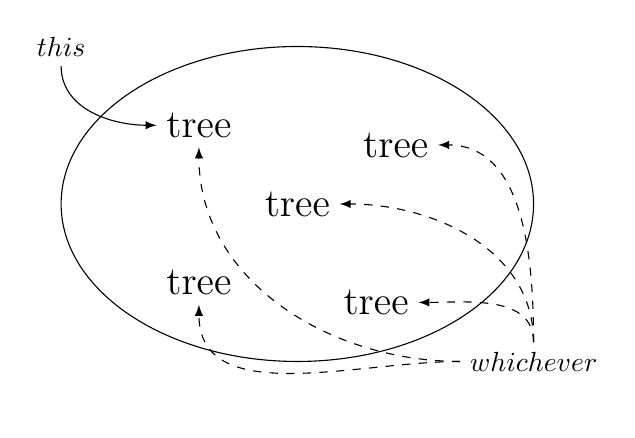
\begin{tikzpicture}
		\node (ellipse)	at (3,2)	{};
		\node (this)	at (0,4)	{$this$};
		\node (some)	at (6,0)	{$whichever$};

		\node (fig_1)	at (2-0.25 , 3+0.00)	{\Large\faicon{tree}};
		\node (fig_2)	at (4+0.25 , 3-0.25)	{\Large\faicon{tree}};
		\node (fig_3)	at (2-0.25 , 1+0.00)	{\Large\faicon{tree}};
		\node (fig_4)	at (4+0.00 , 1-0.25)	{\Large\faicon{tree}};
		\node (fig_5)	at (3-0.00 , 2+0.00)	{\Large\faicon{tree}};

		\draw (ellipse) ellipse [x radius=3, y radius=2];

		\draw[-latex] (this) to [out=south, in=west] (fig_1);
		\draw[-latex, dashed] (some) to [out=west, in=south] (fig_1);
		\draw[-latex, dashed] (some) to [out=north, in=east] (fig_2);
		\draw[-latex, dashed] (some) to [out=west, in=south] (fig_3);
		\draw[-latex, dashed] (some) to [out=north, in=east] (fig_4);
		\draw[-latex, dashed] (some) to [out=north, in=east] (fig_5);
	\end{tikzpicture}
	}
\xe
\end{figure}

\begin{figure}[h]
\begin{morphlex}
\ex\label{ex:memorphlex}%
\adjustbox{valign=t}{%
	\begin{tabu} {\usetabu{morphlexnarrow}}
	\rayr{\larger me/}{mə-}
		& Cl
		& \begin{tabular}[t]{l l l}
			\ups{\Def} & = & $-$ \\
			\ups{\Specif} & = & $-$ \\
		\end{tabular}
	\end{tabu}%
}
\xe
\end{morphlex}
\end{figure}

Since according to \citet[152]{lyons1999}, demonstratives are inherently
definite---and their reference is specific, too---the deictic proclitics
\xayr{Ed/}{eda-}{this}, \xayr{Ad/}{ada-}{that}, and \xayr{d/}{da-}{such} are in
complementary distribution\index{complementary distribution} with the inspecificity marker, as demonstrated by
(\ref{ex:inspecdeix}): neither combination of \rayr{me/}{mə-} and \rayr{Ed/}
{eda-} in (\ref{ex:inspecdeix}cd) results in an ungrammatical sentence because 
\rayr{Ed/}{eda-} encodes [\Def{}~$+$, \Specif{}~$+$] while \rayr{me/}
{mə-} encodes [\Def{}~$-$, \Specif{}~$-$]. Attempting to assign
opposing values to the same feature (\Def{} and \textsc{specific},
respectively) must fail.

\begin{figure}
\pex\label{ex:inspecdeix}
\a\label{ex:inspecdeix_1}\begingl
	\gla Ang @ nakasyon nihanye eda-mehirya. //
	\glb ang= nakas-yon nihan-ye-Ø eda=mehir-ya //
	\glc \AgtT{}= grow-\TplN{} fruit-\Pl{}-\Top{} this=tree-\Loc{} //
	\glft `Fruits are growing on this tree.' //
\endgl

\a\label{ex:inspecdeix_2}\begingl
	\gla Ang @ nakasyon nihanye mə-mehirya. //
	\glb ang= nakas-yon nihan-ye-Ø mə=mehir-ya //
	\glc \AgtT{}= grow-\TplN{} fruit-\Pl{}-\Top{} whichever=tree-\Loc{} //
	\glft `Fruits are growing on whichever tree.' //
\endgl

\a\ljudge*\label{ex:inspecdeix_3}\begingl
	\gla Ang @ nakasyon nihanye mə-eda-mehirya. //
	\glb ang= nakas-yon nihan-ye-Ø mə=eda=mehir-ya //
	\glc \AgtT{} grow-\TplN{} fruit-\Pl{}-\Top{} whichever=this=tree-\Loc{} //
\endgl

\a\ljudge*\label{ex:inspecdeix_4}\begingl
	\gla Ang @ nakasyon nihanye eda-mə-mehirya. //
	\glb ang= nakas-yon nihan-ye-Ø eda=mə=mehir-ya //
	\glc \AgtT{}= grow-\TplN{} fruit-\Pl{}-\Top{} this=whichever=tree-\Loc{} //
\endgl

\xe
\end{figure}

The inspecificity proclitic \rayr{me/}{mə-} cannot commonly be combined with
pronouns, since personal pronouns\index{pronouns!personal} as well as demonstrative pronouns\index{pronouns!demonstrative} have a
definite reference; combining the clitic with an indefinite pronoun\index{pronouns!indefinite} would be
redundant. With interrogative pronouns\index{pronouns!interrogative} it is feasible to use \rayr{me/}{mə-} as
an intensifier\index{intensifiers}, though without the vulgar tone of the English translation given
in (\ref{ex:meinter}).

\begin{figure}[h]
\ex\label{ex:meinter}\begingl
	\gla Amangreng mə-simin? //
	\glb amang=reng mə=simin //
	\glc happen=\TsgI{}.\Aarg{} whichever=how //
	\glft `How the fuck did that happen?' //
\endgl\xe
\end{figure}

\index{clitics|)}
\index{prefixes|)}

\section{Adjective and adverb phrases}
\label{sec:adjps-advps}

Adjectives and adverbs in Ayeri are largely similar in that they can both be
modified by adverbs\index{adverbs} like \fw{very}, and they both modify heads: adjectives\index{adjectives}
modify nouns, adverbs\index{adverbs} modify everything else. \citet{carnie2013} thus urges his
readers to think about whether it is sensible to distinguish between the two
categories \citep[51]{carnie2013}, so let us focus in this section on
structural similarities and dissimilarities between the two, as well as their
distribution as morphemes.

\subsection{Adjective phrases}
\label{subsec:adjps}
\index{adjectives|(}
\index{phrase types!adjective phrase|(}

As described in the previous section, APs usually constitute adjuncts\index{grammatical function!adjunct} of NPs\index{phrase types!noun phrase} or
certain kinds of DPs\index{phrase types!determiner phrase} (demonstratives\index{pronouns!demonstrative}, notably), where they describe properties
of these nominal elements. Adjectives are likewise commonly found as
predicative complements (\Plink{}\index{grammatical function!predicative complement}) in copular clauses\index{copular clause}, compare
\autoref{subsec:eqs}. Possessive pronouns can be used as modifiers as well,
though they are probably still better classified as DP\index{phrase types!determiner phrase} heads. The
phrase-structure rule in (\ref{ex:adjpstruct}) and the c-structure tree in
(\ref{ex:adjpcstruct}) show how an AP is constructed.

\begin{figure}[h]
\pex\label{ex:adjpstruct}
\a AP → \anno*{\xbar{A}} \anno*[\elem{\Adjc}]{AdvP}
\a \xbar{A} → \anno*{\xhead{A}} \anno*[\pass{\GF}]{XP}
\xe
\end{figure}

\begin{figure}[h]
\ex\labels\label{ex:adjpcstruct}
\begin{minipage}[t]{.5\remaining}
\tl\quad%
\begin{forest}
[{\anno[\elem{\Adjc} $\vee$ \pass{\Plink}]{AP}}
	[\anno{\xbar{A}}
		[\anno{\xhead{A}}]
		[{\anno[\pass{\GF}]{XP}}]
	]
	[{\anno[\elem{\Adjc}]{AdvP}}]
]
\end{forest}
\end{minipage}
~
\begin{minipage}[t]{.5\remaining}
\tl\quad%
\begin{forest}
[{\anno[\elem{\Adjc} $\vee$ \pass{\Plink}]{AP}}
	[\anno{AP}
		[\anno{\xhead{A}}]
		[{\anno[\elem{\Adjc}]{AdvP}}]
	]
	[{\anno[\pass{\GF}]{XP}}]
]
\end{forest}
\end{minipage}
\xe
\end{figure}

Adjective phrases have an adjective as their lexical head. This head may be
extended by modifiers adjoined to \xbar{A}; \xbar{A} repeats for the adjunct\index{grammatical function!adjunct}ion
of multiple modifiers. Since modifiers follow\index{word order} their heads here as well, APs are
also a right-branching constituent. Complements of adjectives are subsumed
under the label XP in the phrase structure rules, which here stands for NP\index{phrase types!noun phrase}, DP\index{phrase types!determiner phrase},
and CP\index{phrase types!complementizer phrase}. An example of each phrase type modifying an adjective is given in
(\ref{ex:adjmod}) and (\ref{ex:adjmod2}).

\begin{figure}
\pex\label{ex:adjmod}
\a\label{ex:adjmod_adv}%
	\begin{minipage}[t]{.5\remaining}%
	\begingl
		\glpreamble adjective + AdvP\index{phrase types!adverb phrase} adjunct\index{grammatical function!adjunct}: //
		\gla Adareng bisuayas sadayo kalam. //
		\glb ada-reng bisuay-as sadayo kalam //
		\glc that-\AargI{} idea-\Parg{} crazy truly //
		\glft `That is a truly crazy idea.' //
	\endgl\medskip
	
	\begin{avm}
	\[
		\Obj	&	\[
			\Pred	&	`idea' \\
			\Anim	&	$+$ \\
			\Case	&	\Parg \\
			\Adjc	&	\{\[
				\Pred	&	`crazy` \\
				\Adjc	&	\{\[
					\Pred	&	`truly' \\
				\]\} \\
			\]\} \\
		\]
	\]
	\end{avm}
	\end{minipage}
	\hfill
	\begin{forest} narrower nodes, shorter edges, italic leaves,
	[{\anno[\pass{\Obj}]{NP}}
%		[\anno{\xbar{N}}
			[\anno{\xhead{N}}
				[bisuayas]
			]
			[{\anno[\elem{\Adjc}]{AP}}
%				[\anno{\xbar{A}}
					[\anno{\xhead{A}}
						[sadayo]
					]
					[{\anno[\elem{\Adjc}]{AdvP}}
						[kalam]
					]
%				]
			]
%		]
	]
	\end{forest}

\a\label{ex:adjmod_np}%
	\begin{minipage}[t]{.5\remaining}
	\begingl
		\glpreamble adjective + NP\index{phrase types!noun phrase} complement: //
		\gla Yang mino yanena nā. //
		\glb yang mino yan-ena nā //
		\glc \Fsg{}.\Aarg{} happy son-\Gen{} \Fsg{}.\Gen{} //
		\glft `I am happy about my son.' //
	\endgl\medskip

	\begin{avm}
	\[
		\Plink	&	\[
			\Pred		&	\astruct{happy}{\ups{\Oblq{theme}}} \\
			\Oblq{theme}	&	\[
				\Pred	&	\astruct{son}{\ups{\Possr}} \\
				\Case	&	\Gen \\
				\Possr	&	\[
					% \Pred	&	`$pro$' \\
					% \Case	&	\Gen \\
					% \Num	&	\Sg \\
					% \Pers	&	\First \\
					\avmspan{``my''} \\
				\] \\
			\] \\
		\] \\
	\]
	\end{avm}
	\end{minipage}
	\hfill
	\begin{forest} narrower nodes, shorter edges, italic leaves,
	[{\anno[\pass{\Plink}]{AP}}
%		[\anno{\xbar{A}}
			[\anno{\xhead{A}}
				[mino]
			]
			[{\anno[\pass{\Oblq{theme}}]{NP}}
				[{yanena nā}, roof]
			]
%		]
	]
	\end{forest}
\xe
\end{figure}

\begin{figure}
\pex\label{ex:adjmod2}
\a\label{ex:adjmod_dp}%
	\begin{minipage}[t]{.5\remaining}
	\begingl
		\glpreamble adjective + DP\index{phrase types!determiner phrase} complement: //
		\gla Yang mino yayam. //
		\glb yang mino yayam //
		\glc \Fsg{}.\Aarg{} happy \TsgM{}.\Dat{} //
		\glft `I am happy for him.' //
	\endgl\medskip

	\begin{avm}
	\[
		\Plink	&	\[
			\Pred	&	\astruct{happy}{\ups{\Oblq{ben}}} \\
			\Oblq{ben}	&	\[
				% \Pred	&	`$pro$' \\
				% \Case	&	\Dat \\
				% \Num	&	\Sg \\
				% \Pers	&	\Second \\
				\avmspan{``him''} \\
			\] \\
		\] \\
	\]
	\end{avm}
	\end{minipage}
	\hfill
	\begin{forest} narrower nodes, shorter edges, italic leaves,
	[{\anno[\pass{\Plink}]{AP}}
%		[\anno{\xbar{A}}
			[\anno{\xhead{A}}
				[mino]
			]
			[{\anno[\pass{\Oblq{ben}}]{DP}}
				[yayam]
			]
%		]
	]
	\end{forest}

\a\label{ex:adjmod_cp}%
	\begin{minipage}[t]{.5\remaining}
	\begingl
		\glpreamble adjective + CP\index{phrase types!complementizer phrase} complement: //
		\gla Yang valuy, yomavāng edaya. //
		\glb yang valuy yoma=vāng edaya //
		\glc \Fsg{}.\Aarg{} glad exist=\Second.\Aarg{} here //
		\glft `I am glad that you are here.' //
	\endgl\medskip

	\begin{avm}
	\[
		\Plink	&	\[
			\Pred	&	\astruct{glad}{\ups{\Compl}} \\
			\Compl	&	\[
			% 	\Pred		&	\astruct{exist}{...} \\
			% 	\Subj		&	\[...\] \\
			% 	\Oblq{loc}	&	\[...\] \\
				\avmspan{``you are here''} \\
			\] \\
		\] \\
	\]
	\end{avm}
	\end{minipage}
	\hfill
	\begin{forest} narrower nodes, shorter edges, italic leaves,
	[{\anno[\pass{\Plink}]{AP}}
%		[\anno{\xbar{A}}
			[\anno{\xhead{A}}
				[valuy]
			]
			[{\anno[\pass{\Compl}]{CP}}
				[{yomavāng\\ edaya}, roof]
			]
%		]
	]
	\end{forest}

\xe
\end{figure}

Example (\ref{ex:adjmod_adv}) gives the f- and c-structures for the adjective
phrase to show that \Adjc{}\index{grammatical function!adjunct} may be recursive: an adjective which serves as one
of many modifiers to a noun can itself be modified by adverbs\index{adverbs}. Likewise, an
adjective--adverb\index{adverbs} combination can be complemented by an NP\index{phrase types!noun phrase}, as shown in
(\ref{ex:adjmod_dp}). Especially in (\ref{ex:adjmod_np}) and
(\ref{ex:adjmod_dp}) we can see Ayeri's propensity for using cases\index{case} with
complements where English would use prepositions. Thus, in
(\ref{ex:adjmod_np}), `about' is expressed by putting the nominal complement in
the genitive case\index{case!genitive}: the NP\index{phrase types!noun phrase} complement expresses an oblique\index{grammatical function!oblique} theme\index{semantic role!theme} about which the
experiencing subject becomes happy. This, however, should not be conflated with
a possessor\index{semantic role!possessor}, \Possr{}, but should be labeled separately as an oblique\index{grammatical function!oblique}
complement, \Oblq{theme}\index{semantic role!theme}. Similarly, the recipient\index{semantic role!recipient} of the subject's happiness
appears as an NP\index{phrase types!noun phrase} complement in the (ethical) dative\index{case!dative} in (\ref{ex:adjmod_dp}).
Instrumental and causative NP\index{phrase types!noun phrase} complements instead of PPs\index{phrase types!prepositional phrase} may be found as well
(compare \autoref{subsubsec:valincr}, p.~\pageref{subsubsec:valincr}).
Moreover, according to \citet{carnie2013}, quantifiers\index{quantifiers} or intensifiers\index{intensifiers} of
adjectives are adverbs\index{adverbs}, so they should find themselves in \Adjc{}\index{grammatical function!adjunct}. An example
of this is given in (\ref{ex:adjquant3}).

\begin{figure}[h]
\pex\label{ex:adjquant3}
\a
\begin{minipage}[t]{.5\remaining}
\begingl
	\gla luyu-mas //
	\glb luyu=mas //
	\glc strange=kind.of //
	\glft `kind of strange' //
\endgl
\end{minipage}
~
\begin{avm}
\[
	\Pred	&	`strange' \\
	\Adjc	&	\{\[
					\Pred	&	`kind of' \\
				\]\} \\
\]
\end{avm}

\a\label{ex:adjadvconv}
\begin{minipage}[t]{.5\remaining}
\begingl
	\gla valuy ipan. //
	\glb valuy ipan //
	\glc glad extremely //
	\glft `extremely glad' //
\endgl
\end{minipage}
~
\begin{avm}
\[
	\Pred	&	`glad' \\
	\Adjc	&	\{\[
					\Pred	&	`extremely' \\
				\]\} \\
\]
\end{avm}

\xe
\end{figure}

With regards to complements and adjuncts\index{grammatical function!adjunct} to NP\index{phrase types!noun phrase}, \citet{carnie2013} explains,
\textcquote[182]{carnie2013}{Since complements are sisters to X and not \xbar{X},
they cannot stand next to the word \fw{one}. Adjuncts\index{grammatical function!adjunct}, by definition, can}. To
target \xbar{A} nodes, we need something corresponding to English \fw{so},
which we find in Ayeri \xayr{d/}{da-}{thus, so, such}. Since adverbs\index{adverbs} are
adjuncts\index{grammatical function!adjunct}, it is possible to replace the adjective \xayr{sdyo}{sadayo}{crazy} in
(\ref{ex:soreplacement}a) with \rayr{d/}{da-} in (\ref{ex:soreplacement}b); the
\xbar{A} in (\ref{ex:soreplacement}a) being targeted is the sister to
AdvP\index{phrase types!adverb phrase}.\footnote{Since in \Lfg{}\index{Lexical-functional grammar}, non-branching \xbar{X} nodes are omitted for
brevity, c-structure trees do not strictly distinguish between complements and
adjuncts\index{grammatical function!adjunct} \citep[127, fn. 52]{bresnan2016}; functional annotations provide
information about the status of a node instead. The tree in
(\ref{ex:soreplacement}), however, keeps those \xbar{X} nodes which would
otherwise be omitted.}

\begin{figure}
\ex\label{ex:soreplacement}\labels%
\begin{minipage}[t]{0.5\remaining}%
\tl\quad\begingl%
	\gla bisuayas sadayo kalam //
	\glb bisuay-as sadayo kalam //
	\glc idea-\Parg{} crazy truly //
	\glft `a truly crazy idea' //
\endgl\\[1ex]

\tl\quad\begingl
	\gla Da-kalam bisuayang. //
	\glb da=kalam bisuay-ang //
	\glc so=truly idea-\Aarg{} //
	\glft `The idea is truly so.' //
\endgl
\end{minipage}
~
\begin{forest} shorter edges, italic leaves,
% Superfluous bar levels here are on purpose!
[NP
	[\xbar{N}
		[\xbar{N}
			[\xhead{N}
				[bisuayas]
			]
		]
		[AP
			[\xbar{A}
				[\xbar{A}, name=abar
					[\xhead{A}
						[sadayo]
					]
				]
				[AdvP
					% [\xbar{Adv}
					% 	[\xbar{Adv}
					% 		[\xhead{Adv}
								[kalam]
					% 		]
					% 	]
					% ]
				]
			]
		]
	]
]
%
\draw [latex-] (abar) -- ++(-3em,-3em) coordinate (abarlabel);
\node () at (abarlabel) [anchor=north east] {\emph{so}};
\end{forest}
\xe
\end{figure}

Continuing this replacement test for the other example sentences from
(\ref{ex:adjmod}), we can see that the outcomes are ungrammatical; the NPs\index{phrase types!noun phrase} are
dependent on their lexical head, which cannot be omitted or replaced by a
pro-form. The idiomatic English translations in (\ref{ex:soreplacement_2})
somewhat conceal this. The literal translations try to show that the
complements are more tightly integrated into the sentence in Ayeri than in the
idiomatic translations in an attempt to convey how they must seem non-sensical
to an Ayeri speaker.

\begin{figure}
\pex\label{ex:soreplacement_2}
\a\label{ex:soreplacement_2_1}\ljudge*\begingl
	\gla Yang da-yanena nā. //
	\glb yang da=yan-ena nā //
	\glc \Fsg{}.\Aarg{} so=son-\Gen{} \Fsg{}.\Gen{} //
	\glft `I am so about my son.'\\
		\textit{Literally:} `*I am my son's so.' //
\endgl
\a\label{ex:soreplacement_2_2}\ljudge*\begingl
	\gla Yang da-yayam. //
	\glb yang da=yayam //
	\glc \Fsg{}.\Aarg{} so=\TsgM{}.\Dat{} //
	\glft `I am so for him.' \\
		\textit{Literally:} `*I am him so.' //
\endgl

\a\label{ex:soreplacement_2_3}\ljudge*\begingl
	\gla Yang da-yomavāng edaya. //
	\glb Yang da=yoma=vāng edaya //
	\glc \Fsg{}.\Aarg{} so=exist=\Second{}.\Aarg{} here //
	\glft `*I am so that you are here.' //
\endgl
\xe
\end{figure}

% FIXME: Can this be mitigated by replacing "da-" with a full demonstrative?
% Would the conjunct be interpreted as an adjunct in this case? Why?

Further complications arise with regards to complementation in that non-clitic
quantifiers\index{quantifiers} like \xayr{AMkYu}{ankyu}{really} cause a complement of an adjective
to be pushed further to the right. This may be treated as extraposition\index{word order} of the
complement, and is possibly due to syntactic weight \citep{wechsler2009}.
Example (\ref{ex:intrusivequant}) attempts to illustrate the c-structure for a
displaced CP\index{phrase types!complementizer phrase}. Following the annotation rules in \citet[107]{bresnan2016}, such
an analysis is probably not unproblematic since it is required for the adjoined
phrasal node to be either unannotated or not to embody an argument function,
while \Comp{} is an argument function. Using lexocentric feature annotation is
not possible here, since CPs\index{phrase types!complementizer phrase} cannot be marked for case\index{case}.

\begin{figure}
\ex\label{ex:intrusivequant}%
\begingl[aboveglbskip=1em]
	\gla Yang valuy {\_\tikzmark{intrusivequant2_1}} ankyu, 
	\textup{[ } @ yomavāng edaya\tikzmark{intrusivequant2_2} @ \textup{ ]}. //
	\glb yang valuy {} ankyu {} yoma=vāng edaya {} //
	\glc \Fsg{}.\Aarg{} glad {} really {} exist=\Second{}.\Aarg{} here {} //
	\glft `I am really glad you are here.' //
\endgl
\begin{tikzpicture}[remember picture, overlay]
\draw [-latex] ([xshift=-.25em,yshift=-.75ex]{pic cs:intrusivequant2_1}) 
|- ++ (south:.75em) -| ([xshift=-.5*width("yomavāng edaya"),yshift=-.75ex]{pic
cs:intrusivequant2_2});
\end{tikzpicture}

\begin{forest} shorter edges, italic leaves,
[{\anno[\pass{\Plink}]{AP}}
%	[\anno{\xbar{A}}
		[\anno{AP}
			[\anno{\xbar{A}}
				[\anno{\xhead{A}}
					[valuy]
				]
				[$\epsilon$, name=CP_orig]
			]
			[{\anno[\elem{\Adjc}]{AdvP}}
				[ankyu]
			]
		]
		[{\anno[\pass{\Compl}]{CP}}
			[{yomavāng edaya}, roof, name=CP]
		]
%	]
]
%
\draw [-latex, dashed] (CP_orig) to [out=south, in=south] (CP);
\end{forest}
\xe
\end{figure}

\begin{figure}
\ex\label{ex:intrusivequant_fstruct}
\begin{avm}
\[
	\Plink	&	\[
		\Pred	&	\astruct{glad}{\ups{\Compl}} \\
		\Adjc	&	\{\[
			\Pred	&	`really' \\
		\]\}\\
		\Compl	&	\[
			\Pred	&	\astruct{exist}{\ups{\Subj}, \ups{\Oblq{loc}}} \\
			\Subj	&	\[
				% \Pred	&	`$pro$' \\
				% \Pers	&	\Second \\
				% \Case	&	\Aarg \\
				\avmspan{``you''} \\
			\] \\

			\Oblq{loc}	&	\[
				\Pred	&	`here' \\
			\] \\
		\] \\
	\] \\
\]
\end{avm}
\xe
\end{figure}

As pointed out in \autoref{sec:adjectives}, Ayeri's adjectives inflect very
little, since there is no agreement\index{agreement} morphology. However, there exist
morphological means of comparison\index{comparison} or negation\index{negation}. This is reflected in the
functional annotations given in (\ref{ex:adjmorphlex}). The features \Deg{},
\Degdim{}, and \Neg{} appear in brackets here, since they do not apply
universally: adjectives normally appear in the positive in both regards,
comparison\index{comparison} and polarity, and are morphologically unmarked in these cases.
\Degdim{} also does not play a role here, since there are only clitics\index{clitics} for
positive comparison\index{comparison}, and negative comparison\index{comparison} is achieved by negating the
adjective with the regular negative suffix \rayr{/Oj}{-oy}. Examples of the
different ways an adjective may be morphologically marked and their respective
representation as an \Avm{} are given in (\ref{ex:adjmorph}).

\begin{figure}[h]
\begin{morphlex}
\ex\label{ex:adjmorphlex}%
\adjustbox{valign=t}{%
	\begin{tabu} {\usetabu{morphlexnarrow}}
	...
		& A
		& \begin{tabular}[t]{l @{ } l l l @{ } l}
			  & \ups{\Pred} & = & `...' \\
			( & \ups{\Deg} & = & \{\Pos, \Comp, \Supl\} & ) \\
			( & \ups{\Degdim} & = & \{$equative$, $negative$, $positive$\} 
				& )	\\
			( & \ups{\Neg} & = & $\pm$ & ) \\
		\end{tabular}
	\end{tabu}%
}
\xe
\end{morphlex}
\end{figure}

\begin{figure}
\pex\label{ex:adjmorph}
\a\label{ex:adjmorph_compar}
\begin{minipage}[t]{.5\remaining}
\begingl
	\gla nake-vā //
	\glb nake=vā //
	\glc tall=\Supl{} //
	\glft `tallest' //
\endgl
\end{minipage}
~
\begin{avm}
\[
	\Pred	&	`tall' \\
	\Deg	&	\Supl \\
\]
\end{avm}

\a\label{ex:adjmorph_neg}
\begin{minipage}[t]{.5\remaining}
\begingl
	\gla mingoy //
	\glb ming-oy //
	\glc capable-\Neg{} //
	\glft `incapable' //
\endgl
\end{minipage}
~
\begin{avm}
\[
	\Pred	&	`capable' \\
	\Neg	&	$+$ \\
\]
\end{avm}

\a\label{ex:adjmorph_compar+neg}
\begin{minipage}[t]{.5\remaining}
\begingl
	\gla pasīsoy-eng //
	\glb pasīsa-oy=eng //
	\glc interesting-\Neg{}=\Comp{} //
	\glft `more uninteresting' //
\endgl
\end{minipage}
~
\begin{avm}
\[
	\Pred	&	`interesting' \\
	\Deg	&	\Comp \\
	\Neg	&	$+$ \\
\]
\end{avm}

\xe
\end{figure}

We have already seen above (\autoref{subsec:adjcomp}) that the morphemes used
for synthetic\index{synthesis} comparison\index{comparison} of adjectives are grammaticalized clitics literally
meaning `rather, more' (\rayr{/ENF}{-eng}) and `most' (\rayr{/vaa}{-vā}) as
lexical quantifiers\index{quantifiers}. With adjectives, there is no clear-cut line between their
functional and their lexical use. I have analyzed them here as functional,
since they may be interpreted as such, depending on context.

\index{adjectives|)}
\index{phrase types!adjective phrase|)}

\subsection{Adverb phrases}
\label{subsec:advps}
\index{adverbs|(}
\index{phrase types!adverb phrase|(}

Adverbs, as (\ref{ex:adjadvconv}) shows, can easily be converted from
adjectives\index{adjectives}. Thus, \xayr{IpnF}{ipan}{extreme}, which is normally an adjective\index{adjectives},
is used there in an adverbial way, meaning `extremely'. The word stays the
same, however: \rayr{IpnF}{ipan}, without a derivative\index{derivation} affix akin to English
\fw{-ly} or French\index{French} \fw{-ment}. Since adverbs and adjectives\index{adjectives} are functionally
similar, \citet{carnie2013} poses the question whether adjectives\index{adjectives} and adverbs
should rather be analyzed as being part of the same category. He reasons that

\blockcquote[51]{carnie2013}{[b]oth Adj and Adv can be modified by the word
\fw{very}, and they both have the same basic function in the grammar---to
attribute properties to the items they modify. In fact, the only major
distinction between them is syntactic: Adjectives\index{adjectives} appear inside NPs\index{phrase types!noun phrase}, while
adverbs appear elsewhere.}

Adjectives\index{adjectives} and adverbs are in complementary distribution, which, he writes,
would normally be taken as evidence that these two things are of the same
category. In fact, the only reason \citet{carnie2013} adduces for keeping the
two categories apart is \textquote{because they are familiar to most people,}
and he prompts the reader to consider that uniting them in a single
supercategory \textcquote[51]{carnie2013}{might provide a better analysis and
might be better motivated scientifically}. \citet[126]{bresnan2016} also
classify both adjectives\index{adjectives} and adverbs as heads of AP\index{phrase types!adjective phrase} with reference to
\citet{emonds1976}. As described in \autoref{sec:adverbs}, the only morphology
attributive adverbs take in Ayeri is comparison\index{comparison} morphology and negation\index{negation}. This
is the same as with adjectives\index{adjectives} indeed, hence the morpholexic specifications
in (\ref{ex:advmorphlex}) appear equal.

\begin{figure}[h]
\begin{morphlex}
\ex\label{ex:advmorphlex}%
\adjustbox{valign=t}{%
	\begin{tabu} {\usetabu{morphlexnarrow}}
	...
		& A
		& \begin{tabular}[t]{l @{ } l l l @{ } l}
			  & \ups{\Pred} & = & `...' \\
			( & \ups{\Deg} & = & \{\Comp, \Supl\} & ) \\
			( & \ups{\Neg} & = & $+$ & ) \\
		\end{tabular}
	\end{tabu}%
}
\xe
\end{morphlex}
\end{figure}

If we look at the phrase structure (\ref{ex:advpstruct}) and the c-structure
(\ref{ex:advpcstruct}) for adverbs, however, there is a slight difference in
that adverbs\index{adverbs} cannot serve as \Plink{}\index{grammatical function!predicative complement} in equative statements; they also can
only be modified by other adverbs, and they cannot take complements.%
\footnote{For adjectives\index{adjectives}, compare (\ref{ex:adjpstruct}),
(\ref{ex:adjpcstruct}), and (\ref{ex:adjmorphlex}) in \autoref{subsec:adjps}.}
On the other hand, adjectives\index{adjectives} are restricted to nominal contexts whereas
adverbs may modify any other lexical category: verbs\index{verbs}, adjectives\index{adjectives}, prepositions\index{adpositions!prepositions},
as well as other adverbs.

\begin{figure}[h]
\ex\label{ex:advpstruct}
AdvP → \anno*{\xhead{Adv}} \anno*[{\elem{\Adjc}}]{AdvP}
\xe
\end{figure}

\begin{figure}[h]
\ex~\label{ex:advpcstruct}\labels
\begin{forest}
[{\anno[\elem{\Adjc}]{AdvP}}
%	[\anno{\xbar{Adv}}
		[\anno{\xhead{Adv}}]
		[{\anno[{\elem{\Adjc}}]{AdvP}}]
%	]
]
\end{forest}
\xe
\end{figure}

Example (\ref{ex:advmod}) illustrates various modifiers of adverbs. These
modifiers are often quantifying\index{quantifiers}/intensifying adverbs, whether clitic\index{clitics} ones or
free ones. Since adjectives\index{adjectives} and adverbs are not distinguished by morphology,
the heads of both phrases, \xayr{vkis}{vakisa}{careful} and \xayr{bit}{bita}
{ordinary, normal}, may be interpreted as adjectives\index{adjectives} as well, depending on
context.

\begin{figure}
\pex\label{ex:advmod}
\a\label{ex:advmod_free}%
\begin{minipage}[t]{.667\remaining}%
\begingl
	\gla bita ikan-ikan //
	\glb bita ikan.ikan //
	\glc ordinarily completely //
	\glft `completely ordinarily' //
\endgl~\\

\begin{avm}
\[
	\Adjc	&	\{\[
		\Pred	&	`ordinarily' \\
		\Adjc	&	\{\[
			\Pred	&	`completely' \\
		\]\} \\
	\]\} \\
\]
\end{avm}
\end{minipage}
~
\begin{forest} shorter edges, italic leaves,
[{\anno[\elem{\Adjc}]{AdvP}}
%	[\anno{\xbar{Adv}}
		[\anno{\xhead{Adv}}
			[bita]
		]
		[{\anno[\elem{\Adjc}]{AdvP}}
%			[\anno{\xbar{Adv}}
%				[\anno{\xhead{Adv}}
					[ikan-ikan]
%				]
%			]
		]
%	]
]
\end{forest}

\a\label{ex:advmod_clitic}%
\begin{minipage}[t]{.667\remaining}%
\begingl
	\gla vakisoy @ -ma //
	\glb vakisa-oy =ma //
	\glc carefully-\Neg{} =enough //
	\glft `not carefully enough' //
\endgl~\\

\begin{avm}
\[
	\Adjc	&	\{\[
		\Pred	&	`carefully' \\
		\Neg	&	$+$ \\
		\Adjc	&	\{\[
			\Pred	&	`enough' \\
		\]\} \\
	\]\} \\
\]
\end{avm}
\end{minipage}
~
\begin{forest} shorter edges, italic leaves,
[{\anno[\elem{\Adjc}]{AdvP}}
%	[\anno{\xbar{Adv}}
		[\anno{\xhead{Adv}}
			[\anno{\xhead{Adv}}
				[vakisoy]
			]
			[{\anno[\elem{\Adjc}]{Cl}}
				[-ma]
			]
		]
%	]
]
\end{forest}
\xe
\end{figure}

Clitic\index{clitics} quantifiers\index{quantifiers}, as in (\ref{ex:advmod_clitic}), attach immediately to the
head they modify rather than to the last word of the AdvP. It may be assumed
that the functional scheme given in (\ref{ex:advmorphlex}) also holds for them.
\citet{carnie2013} at least treats all modifiers of adjectives\index{adjectives} and adverbs as
adverbs. Even though these usually refer to the extent of the adjective\index{adjectives} or
adverb, they differ from quantifiers\index{quantifiers} of nouns, which were analyzed above as
determiners encoding the \Quant{} feature rather than being plain adjectives\index{adjectives}.
Quantifiers\index{quantifiers} of adjectives\index{adjectives} and adverbs are also able to be modified in turn, as
illustrated by (\ref{ex:clitics_55}) from \autoref{clitics_quant} (compare
p.~\pageref{ex:clitics_55}), which is repeated again here, abbreviated.
\xayr{/IknF}{ikan}{much, many, very} is modified in this case by
\xayr{kgnF}{kagan}{far too} to convey the meaning `far too many'.

\begin{figure}[h]
\ex\label{ex:clitics_55_short}%
\begingl
	\gla keynam @ -ikan kagan //
	\glb keynam-Ø =ikan kagan //
	\glc people-\Top{} =many far.too //
	\glft `far too many people' //
\endgl
\xe
\end{figure}

Besides the parenthetical insertion tests on \rayr{kgnF}{kagan} in
\autoref{clitics_quant}, the examples in (\ref{ex:quantadvcomptest}) show that
\rayr{kgnF}{kagan} also cannot swap places with other nominal modifiers without
a change in meaning (\ref{ex:quantadvcomptest_1}), that \rayr{kgnF}{kagan} does
not work when the rest of the NP\index{phrase types!noun phrase} is replaced by an anaphora
(\ref{ex:quantadvcomptest_2}), and that \rayr{/IknF}{-ikan} cannot be replaced
by an anaphora either (\ref{ex:quantadvcomptest_3}). It appears that
\rayr{kgnF}{kagan} is dependent on \rayr{/IknF}{ikan}, and that
\rayr{/IknF}{-ikan} has head-like qualities with regards to modification by
\rayr{kgnF}{kagan}.

\begin{figure}
\pex\label{ex:quantadvcomptest}
\a\ljudge\excl\label{ex:quantadvcomptest_1}\begingl
	\gla keynam-ikan gino kagan //
	\glb keynam=ikan gino kagan //
	\glc people=many drunk far.too //
	\glft `many far too drunk people'\\
		\textit{Intended:} `far too many drunk people' //
\endgl

\a\ljudge*\label{ex:quantadvcomptest_2}\begingl
	\gla tas kagan //
	\glb tas kagan //
	\glc \TplM{}.\Parg{} far.too //
	\glft `*far too of them' //
\endgl

\a\ljudge*\label{ex:quantadvcomptest_3}\begingl
	\gla keynam da-kagan //
	\glb keynam da=kagan //
	\glc people so=far.too //
	\glft `*far too so people' //
\endgl

\xe
\end{figure}

As (\ref{ex:quantadvcomptest_1}) shows, \xayr{kgnF}{kagan}{far too} and,
alternatively, \xayr{EkeNF}{ekeng}{too} also work with regular adjectives\index{adjectives}, and
it is possible as well to add further adjuncts\index{grammatical function!adjunct} to the AdvP, for instance,
\xayr{ptu}{patu}{surprisingly} in (\ref{ex:kgnadj}). The AP\index{phrase types!adjective phrase} in this example,
\xayr{kejnmF/IknF gino kgnF ptu}{keynam-ikan kagan patu}{many surprisingly far
too drunk people}, has been interpreted to the effect that both
\rayr{kgnF}{kagan} and \rayr{ptu}{patu} modify \rayr{gino}{gino}, rather than
\rayr{ptu}{patu} modifying \rayr{kgnF}{kagan}. Evidence for such an analysis is
provided by \xayr{d/ptu}{da-patu}{surprisingly so} being grammatical, while
*\xayr{gino d/ptu}{gino da-patu}{*surprisingly so drunk} not being so.
\rayr{ptu}{patu} thus must be adjoined to \xbar{A} rather than an \xbar{Adv}
projected by \rayr{kgnF}{kagan}.

\begin{figure}
\pex\label{ex:kgnadj}
\a\label{ex:kgnadj_avm}\begin{avm}
\[
	\Pred	&	`people' \\
	... \\
	\Quant	&	\[
		\Pred	&	`many' \\
	\]\\
	\Adjc	&	\{
		\[
			\Pred	&	`drunk' \\
			\Adjc	&	\{\[
				\Pred	&	`far too' \\
			\] \\
			\[
				\Pred	&	`surprisingly' \\
			\]\} \\
		\]\\
	\} \\
\]
\end{avm}

\a\label{ex:kgnadj_cstruct}\begin{forest} shorter edges, italic leaves,
[{\anno[\pass{\Top{}}]{NP}}
%	[\anno{\xbar{N}}
		[\anno{\xhead{N}}
			[\anno{\xhead{N}}
				[keynam]
			]
			[\anno{Cl}
				[-ikan]
			]
		]
		[{\anno[\elem{\Adjc}]{AP}}
			[\anno{\xbar{A}}
				[\anno{\xhead{A}}
					[gino]
				]
				[{\anno[\elem{\Adjc}]{AdvP}}
					[kagan]
				]
			]
			[{\anno[\elem{\Adjc}]{AdvP}}
				[patu]
			]
		]
%	]
]
\end{forest}
\xe
\end{figure}

\index{phrase types!adverb phrase|)}
\index{adverbs|)}

\section{Prepositional phrases}
\label{sec:pps}
\index{adpositions|(}
\index{phrase types!prepositional phrase|(}

As described in the section on the morphology of adpositions
(\autoref{sec:adpositions}), Ayeri possesses both prepositions and
postpositions, though the former are a lot more common and basic than the
latter. Thus, PPs are an exceptional domain in that very limited left-branching
is possible insofar as the complement of a postposition precedes\index{word order} its head. The
complement of a postposition is, in itself, right-branching again, however.
Since the label `AP' for a more general `adpositional phrase' has already been
used for `adjective\index{adjectives} phrase'\index{phrase types!adjective phrase}, I will use the common label `PP' to refer to both
prepositional and postpositional phrases, with their respective heads referred
to as `\xhead{P}'. It was mentioned earlier that there is no morphological
difference between prepositions and postpositions; head placement is a
syntactic issue and the preference of placement is rooted in the lexical entry
for each adposition.

\Lfg{}\index{Lexical-functional grammar} categorizes PPs as oblique\index{grammatical function!oblique} functions 
\Oblique{}, where $\theta$ stands for the thematic role of the phrase
\citep[9--10]{dalrymple2001}. As we have seen in the previous chapter,
adpositions in Ayeri usually allow adpositional objects\index{grammatical function!adpositional object} to be either marked for
locative\index{case!locative} or dative case\index{case!dative}:

\begin{description}
	\item[Locative:] Standard case\index{case} for adpositional objects\index{grammatical function!adpositional object}, indicates a
	location (\textsc{location}). It usually corresponds to English `at', `in'.
	It is also used for the goal\index{semantic role!goal} (\textsc{goal}) of verbs\index{verbs} of motion when they
	are directed, such as \xayr{sr/}{sara-}{go}, and for the addressee of verbs\index{verbs}
	of speaking like \xayr{nr/}{nara}{speak}. Thus, limitedly, it may also
	express `to'.

	\item[Dative:] Indicates motion along a path towards the direction the
	adposition indicates (\textsc{goal}\index{semantic role!goal}, \textsc{direction}). It usually
	corresponds to English `to', `for'. NPs\index{phrase types!noun phrase} may be marked with dative case\index{case!dative}
	freely to indicate direction without being goverened by an adposition.

	\item[Genitive:] Indicates motion along a path from somewhere 
	(\textsc{source}\index{semantic role!source}). NPs\index{phrase types!noun phrase} may be marked with genitive case\index{case!genitive} freely to indicate
	direction without being goverened by an adposition. Genitive case\index{case!genitive} usually
	corresponds to English `from' or `of' in those cases\index{case}. Genitive case\index{case!genitive} also
	marks secondary themes\index{semantic role!theme}, corresponding to English `about'.
\end{description}

\begin{figure}
\ex\label{ex:talkcstruct}%
English:\\
% \fw{John talks to Mary.} \\

\begin{forest} shorter edges, italic leaves,
[IP
	[{\anno[\pass{\Subj}]{NP}}
		[John]
	]
	[\anno{\xbar{I}}
		[\anno{\xhead{I}}
			[talks]
		]
		[\anno{VP}
			[{\anno[\ups{\downs{\PCase}}]{PP}}
				[\anno{\xhead{P}}
					[to]
				]
				[\anno{NP}
					[Mary]
				]
			]
		]
	]
]
\end{forest}
\hfill
\begin{avm}
\[
	\Pred	&	\astruct{talk}{%
		\ups{\Subj},
		\ups{\Oblq{goal}}
	} \\

	\Subj	&	\[
		\Pred	&	`John' \\
		\Pers	&	\Third \\
	\]\\

	\Oblq{goal}	&	\[
		\Pred	&	`Mary' \\
		\PCase	&	\Oblq{goal} \\
	\]\\
\]
\end{avm}
\xe
\end{figure}

Where English uses a preposition together with the verb\index{verbs} to mark an oblique\index{grammatical function!oblique}
argument, Ayeri usually uses case\index{case}. The case\index{case}
for English is illustrated by (\ref{ex:talkcstruct}). Ayeri, in contrast to
English, often uses an NP\index{phrase types!noun phrase} complement marked with one of the cases\index{case} in the list
above, compare (\ref{ex:naracstruct}). In the case of \xayr{nr/}{nara-}{speak,
talk}, the complement appears in the locative case\index{case!locative}, but as an NP\index{phrase types!noun phrase}, not as a PP.
Thus, there is no \PCase{} attribute necessary here, since there is no
preposition to indicate the relation of the complement to the verb\index{verbs} because case\index{case}
marking accomplishes this function.

Which oblique\index{grammatical function!oblique} case\index{case} the complement appears in is determined by the a-structure
of the verb\index{verbs}, not by the semantics of the complement (compare 
\autoref{subsec:comptr}). Since the dative\index{case!dative} is also used for the
\textsc{beneficiary}\index{semantic role!beneficiary} role, the argument expressing the direction of the talking
appears exceptionally in the locative\index{case!locative} here. In (\ref{ex:naracstruct}) it may
seem as though \rayr{y}{ya} is a preposition---which is a reasonable assumption
about its history. However, it has been established previously that preposed
case\index{case} markers are proclitics (see \autoref{clitics_prenoun_case}, 
p.~\pageref{clitics_prenoun_case}). \rayr{y}{ya} is a case\index{case} marker, not a
preposition; `at/to Pila' is thus \rayr{y pil}{ya Pila}, not *\rayr{y pily}{*ya
Pilaya} with additional locative\index{case!locative} marking on the noun.

\begin{figure}
\ex\label{ex:naracstruct}%
\begingl
\gla Ang @ naraya {} @ Ajān ya @ Pila. //
\glb ang= nara-ya Ø= Ajān ya= Pila //
\glc \AgtT{}= talk-\TsgM{} \Top{}= Ajān \Loc{}= Pila //
\glft `Ajān talks to Pila.' //
\endgl\medskip

\begin{forest} narrower nodes, shorter edges, italic leaves,
[IP
%	[\anno{\xbar{I}}
		[\anno{\xhead{I}}
			[{Ang naraya}, roof]
		]
%	]
	[\anno{S}
		[{\anno[\pass{\Top}]{NP}}
			[Ajān]
		]
		[\anno{VP}
%			[\anno{\xbar{V}}
				[{\anno[\pass{\Oblq{loc}}]{NP}}
					[{ya Pila}]
				]
%			]
		]
	]
]
\end{forest}
\hfill
\begin{avm}
\[
	\Pred	&	\astruct{talk}{%
		\ups{\Subj},
		\ups{\Oblq{loc}}%
	} \\

	\Top	&	\[
		\Pred	&	`Ajān' \\
		\Anim	&	$+$ \\
		\Case	&	\Aarg \\
		\Pers	&	\Third \\
	\] \tikzmark{naracstruct_top} \\

	\Subj	&	\tikzmark{naracstruct_subj} \\

	\Oblq{loc}	&	\[
		\Pred	&	`Pila' \\
		\Case	&	\Loc{} \\
	\]\\
\]
\end{avm}
\begin{tikzpicture}[remember picture, overlay]
\draw [rounded corners=1ex] ([yshift=1ex]{pic cs:naracstruct_top})
	-- ++(east:1em) |- ([yshift=1ex]{pic cs:naracstruct_subj}););
\end{tikzpicture}

\xe
\end{figure}

In Ayeri, PPs proper may either be locative\index{case!locative} complements of the verb\index{verbs} as in
(\ref{ex:naracstruct}) or free locative adverbials, ungoverned by the verb\index{verbs},
though the number of verbs\index{verbs} taking PP complements is smaller than in English due
to case\index{case} marking, as described above. As mentioned initially, Ayeri possesses
prepositions as well as postpositions\index{adpositions!postpositions}. With regards to word order\index{word order} typology, we
can thus note:

\ex
Order of noun and adposition: Adp N, N Adp
\xe

The fact that Ayeri has both prepositions and postpositions\index{adpositions!postpositions} is also reflected
in the phrase structure rules given in (\ref{ex:pppstruct}). Here, the comma
indicates that the two phrases joined by it can occur in either order. Since
there are no circumpositions in Ayeri, only ever one site is occupied. XP is
used again as a catch-all term for various phrase types which form complements
of semantic adpositions in the form of NPs\index{phrase types!noun phrase} and DPs\index{phrase types!determiner phrase}, but especially the
postposition\index{adpositions!postpositions} \xayr{pesnF}{pesan}{until} may also have a CP\index{phrase types!complementizer phrase} complement, that is,
a whole complement clause\index{complement clause}. The nominal complements are objects\index{grammatical function!adpositional object} governed by the
adposition.

\begin{figure}[h]
\pex\label{ex:pppstruct}
\a PP → \anno*{\xbar{P}} \anno*[\elem{\Adjc}]{AdvP}
\a \xbar{P} → \anno*{\xhead{P}}, \anno*[%
	\pass{\Obj{}} $\vee$ \pass{\Compl{}}%
	]{XP}
\xe
\end{figure}

The same as in (\ref{ex:pppstruct}) is spelled out again in c-tree form in
(\ref{ex:ppcstruct}). Prepositional phrases, if not subcategorized for by the
verb\index{verbs}, are optional information and thus not governed by the verb\index{verbs}; the
respective PP is thus part of the set of adjuncts\index{grammatical function!adjunct}. Some verbs\index{verbs}, like
\xayr{tpY/}{tapy-}{put}, may take PP complements headed by an adposition, for
instance, in cases like \fw{Mary puts the book {\normalfont [\tsub{PP}~[%
\tsub{P}} on {\normalfont]~[\tsub{NP}} the pile {\normalfont ]]}}. The PP
\fw{on the pile} is not an adjunct here because \fw{She does so on the pile}
makes no sense; the PP must be an argument of the verb\index{verbs} in this case, not
additional, optional information (again, compare \autoref{subsec:comptr}).
Ayeri behaves the same way in this regard. These governed PPs are categorized
as \Oblique{}\index{grammatical function!oblique} with $\theta$ replaced by the proper semantic role
(\textit{loc}\index{semantic role!location}, \textit{goal}\index{semantic role!goal}, or \textit{src}\index{semantic role!source}).

\begin{figure}
\pex\label{ex:ppcstruct}
\a\begin{forest} shorter edges,
[{\anno[\pass{\downs{\PCase}} $\vee$ \elem{\Adjc} $\vee$ \pass{\Plink}]{PP}}
%	[\anno{\xbar{P}}
		[\anno{\xbar{P}}
			[\anno{\xhead{P}}]
			[{,}, no edge]
			[{\anno[{\pass{\Obj{}} $\vee$ \pass{\Compl{}}}]{XP}}]
		]
		[{\anno[\elem{\Adjc}]{AdvP}}]
%	]
]
\end{forest}

\a\begin{forest} shorter edges,
[{\anno[\pass{\downs{\PCase}} $\vee$ \elem{\Adjc} $\vee$ \pass{\Plink}]{PP}}
	[\anno{PP}
		[\anno{\xhead{P}}]
		[{\anno[\elem{\Adjc}]{AdvP}}]
	]
	[{\anno[{\pass{\Obj{}} $\vee$ \pass{\Compl{}}}]{XP}}]
]
\end{forest}
\xe
\end{figure}

Regarding functional structure, the difference between preposition and
postposition\index{adpositions!postpositions} is meaningless, so the morpholexical definitions in
(\ref{ex:adpmorphlex}) do not distinguish formally between pre- and
postpositions\index{adpositions!postpositions}. As described in \autoref{clitics_prep_dyn}
(p.~\pageref{clitics_prep_dyn}) and \autoref{sec:adpositions}, there is a
particle \rayr{mN}{manga} which has been analyzed as a clitic\index{clitics}. This particle
indicates that an adposition has a directional reading (specifically, into the
direction of the preposition) instead of a locational one. The rule on the
adpositional object's\index{grammatical function!adpositional object} case\index{case} in (\ref{ex:adpmorphlex_1}) excludes
\rayr{liNF}{ling} and \rayr{AvnF}{avan}, which require special treatment with
regards to case\index{case} marking, as described below.

\begin{figure}[h]
\begin{morphlex}
\pex\label{ex:adpmorphlex}%
\a\label{ex:adpmorphlex_1}\adjustbox{valign=t}{%
	\begin{tabu} {\usetabu{morphlex}}
	...
		& P
		& \begin{tabular}[t]{l l l}
			\ups{\Pred} & = & \astruct{...}{\ups{\Obj}} \\
			\ups{\PCase} & = & \{\Oblq{loc}, \Oblq{goal}, \Oblq{src}\} \\
			\ups{\PSem} & = & $loc$ \\
			\ups{\Obj{} \Case{}} & \req & \Loc{}
		\end{tabular}
	\end{tabu}%
}

\a\adjustbox{valign=t}{%
	\begin{tabu} {\usetabu{morphlex}}
	\rayr{\larger mN}{manga}
		& Cl
		& \begin{tabular}[t]{l l l}
			\ups{\PSem} & = & $dir$ \\
			\ups{\PCase} & = & \Oblq{goal} \\
		\end{tabular}
	\end{tabu}%
}
\xe
\end{morphlex}
\end{figure}

German\index{German}, for one, encodes the difference between locational and directional uses
of a group of prepositions as well, but by an alternation in the prepositional
object's case\index{case} between \Dat{} (locational) and \Acc{} (directional). Thus,
\fw{auf dem tisch} (on \Def{}.\Dat{}.\M{}.\Sg{} table) means `on the table',
whereas \fw{auf den tisch} (on \Def{}.\Acc{}.\M {}.\Sg{} table) means `onto the
table'. \citet{butt2005} defines this alternation (albeit for \fw{in} `in' and
\fw{an} `at') as in (\ref{ex:gercasealt}).

\begin{figure}[h]
\ex\label{ex:gercasealt}%
German \citep{butt2005}:\medskip\\
\begin{tabular}[t]{@{} l @{ $\implies$ } l}
\PSem{} $dir$ & \ups{\Obj{} \Case{}} \req{} \Acc{} \\
\PSem{} $loc$ & \ups{\Obj{} \Case{}} \req{} \Dat{} \\
\end{tabular}
\xe
\end{figure}

The \PSem{} feature thus determines the reading of the prepositional object by
a requirement that its case\index{case} be either \Acc{} or \Dat{}, respectively.
Since nouns in German\index{German} always carry case\index{case}, the \PSem{} attribute needs to be
present in the lexical rules for all prepositions which show the \Acc{}/\Dat{}
alternation. %\footnote{These are: 
%\fw{an},
%\fw{auf},
%\fw{hinter},
%\fw{in},
%\fw{neben},
%\fw{über},
%\fw{unter},
%\fw{vor},
%\fw{zwischen}%
%}
In Ayeri, however, the particle \rayr{mN} {manga} alternates with nothing, so
the absence of marking $dir$ indicates a locational reading $loc$\index{semantic role!location} as the
default\index{default}. Different than in German\index{German}, the presence or absence of directionality
marking also does not influence the case\index{case} of the adpositional object\index{grammatical function!adpositional object}.

Example (\ref{ex:mangaaltern}) illustrates the alternation in annotation
between a bare adposition and one modified by \rayr{mN}{manga}:
\rayr{mN}{manga} changes the value of the \PSem{} feature of the f-structure
predicated by the adposition to $dir$ and the \PCase{} feature to \Oblq{goal}\index{semantic role!goal},
as illustrated in (\ref{ex:mangaaltern_marked}). This is how the difference
between locational `in' and directional `into' is represented here. The case\index{case} of
the prepositional object\index{grammatical function!adpositional object} is \Loc{} in both versions of the sentence.

\begin{figure}
\pex\label{ex:mangaaltern}
\a\label{ex:mangaaltern_bare}
\begin{minipage}[t]{.5\remaining}
\begingl
	\gla kong nangaya //
	\glb kong nanga-ya //
	\glc inside house-\Loc //
	\glft `in the house' //
\endgl
\end{minipage}
\hfill
\begin{avm}
\[\Adjc	&	\{\[
		\Pred	&	\astruct{inside}{\ups{\Obj}} \\
		\PCase	&	\Oblq{loc} \\
		\PSem	&	$loc$ \\
		\Obj	&	\[
			\Pred	&	`house' \\
			\Case	&	\Loc \\
		\]
	\]\}
\]
\end{avm}

\a\label{ex:mangaaltern_marked}
\begin{minipage}[t]{.5\remaining}
\begingl
	\gla manga kong nangaya //
	\glb manga kong nanga-ya //
	\glc \Dir{} inside house-\Loc{} //
	\glft `into the house' //
\endgl
\end{minipage}
\hfill
\begin{avm}
\[\Adjc	&	\{\[
		\Pred	&	\astruct{inside}{\ups{\Obj}} \\
		\PCase	&	\Oblq{goal} \\
		\PSem	&	$dir$ \\
		\Obj	&	\[
			\Pred	&	`house' \\
			\Case	&	\Loc \\
		\]
	\]\}
\]
\end{avm}

\xe
\end{figure}

\phantomsection\label{phsec:lingavandat}
With the prepositions \xayr{liNF}{ling}{on top of} and \xayr{AvnF}{avan}{at the
bottom of} there is another alternation, based on case\index{case}, for verbs\index{verbs} which do not
encode direction. This is rooted in the etymology of these words:
\rayr{liNF}{ling} as a noun means `top', \rayr{AvnF}{avan} means `ground,
bottom'. The directional variants of these prepositions mean `to the top, onto'
and `to the bottom'. These are essentially telic\index{telicity} in that they express the
possibility of arriving at the destination specified by the adpositional
object\index{grammatical function!adpositional object}. However, Ayeri does not possess separate adpositions to express `up'
and `down' as `atelic'\index{telicity} concepts, that is, without referring to arriving at a
destination.\footnote{The chosen terminology is possibly slightly problematic
since, strictly speaking, `up' and `down' are also directions rather than
locations.} Instead, \rayr{liNF}{ling} and \rayr{AvnF}{avan} double for `up'
and `down' with dative\index{case!dative} complements, respectively, to mark the difference,
compare \autoref{tab:updowncompl} and \autoref{fig:updowncompl}. Note, however,
that Ayeri does not possess intransitive adpositions, with the exception of a
few verbs\index{verbs} where the adposition is a lexicalized part of the expression, for
instance, \xayr{tpYF/ djrinF}{tapy- dayrin}{save (assets)}, with the
fossilized, now defunct preposition \xayr{djrinF}{dayrin}{beside, next to}
(modern \rayr{kjvo} {kayvo}). `Up' and `down' thus refer to their transitive
uses as in \fw{up the stairs} and \fw{down the hill}, respectively. 
(\ref{ex:dirtel}) provides example sentences for all configurations.

\begin{table}\centering
\caption{Case alternations of \rayr{liNF}{ling} and \rayr{AvnF}{avan}}

\begin{tabu} to \linewidth {X X[c] X[c]}
\toprule\tableheaderfont

%
	& +~\Loc
	& +~\Dat
	\\

\toprule

\tayr{ling}{top}
	& on top of
	& up
	\\

% \midrule

\tayr{manga ling}{to top}
	& to the top of
	& up to
	\\

\midrule

\tayr{avan}{bottom}
	& at the bottom of
	& down
	\\

% \midrule

\tayr{manga avan}{to bottom}
	& to the bottom of
	& down to
	\\

\bottomrule
\end{tabu}

\label{tab:updowncompl}
\end{table}

\begin{figure}\centering
\begin{tikzpicture}[every node/.style={font=\footnotesize\sffamily}]
% Rectangle at bottom
\draw (0,0) rectangle (9,1);

% Rectangle at top
\draw (2.5,2.5) rectangle (6.5,3);

% Ceiling
\draw [line width=.5ex] (0,5) -- (9,5);

% Floor
\draw [line width=.5ex] (0,0) -- (9,0);

% Nodes at bottom, centered over constituent squares
\node (b1) at ($(0,1)!0.5!(1,1)$) {};
\node (b2) at ($(4,1)!0.5!(5,1)$) {};
\node (b3) at ($(8,1)!0.5!(9,1)$) {};

% Nodes at top, centered over constituent squares
\node (t1) at ($(3,3)!0.5!(4,3)$) {};
\node (t2) at ($(4,3)!0.5!(5,3)$) {};
\node (t3) at ($(5,3)!0.5!(6,3)$) {};

% Nodes yonder (top/bottom)
\node (yt)  at ($(0,5)!0.5!(1,5)$) {};
\node (yt2) at ($(-1,6)!0.5!(0,6)$) {};
\node (yb)  at ($(7,0)!0.5!(8,0)$) {};
\node (yb2) at ($(9,-1)!0.5!(10,-1)$) {};

\begin{scope}[nodes={circle, anchor=south, minimum size=2em}]
% Circles on bottom
\node [draw, dashed] (B1) at (b1) {};
\node [fill]         (B2) at (b2) {};
\node [fill]         (B3) at (b3) {};

% Circles on top
\node [fill]         (T1) at (t1) {};
\node [fill]         (T2) at (t2) {};
\node [draw, dashed] (T3) at (t3) {};

% Squares yonder
\node [rectangle, fill] (Y1) at (yt) {};
\node [rectangle, fill] (Y2) [anchor=north] at (yb) {};
\end{scope}

% Arrows from B1
\draw [-{latex[sep=2pt]}] (B1) to [out=north, in=north]
	node [align=center, sloped, above]
		{\fw{manga ling}\\ +\,\Loc}
	(T1);

\draw [-{latex[sep=1em]}] (B1) to [out=north, in=south]
	node [align=center, sloped, above]
		{\fw{manga ling} + \Dat}
	(yt);

\draw [-latex] (B1) to [out=north west, in=south]
	node [align=center, sloped, below]
		{\rotatebox{180}{\fw{ling} + \Dat}}
	(yt2);

% Arrows from T3
\draw [-{latex[sep=2pt]}] (T3) to [out=north east, in=north]
	node [align=center, sloped, above]
		{\fw{manga avan}\\ +\,\Loc}
	(B3);

\draw [-{latex[sep=1em]}] (T3) to [out=north east, in=north]
	node [align=center, sloped, above, pos=.6]
		{\fw{manga avan} + \Dat}
	(yb);

\draw [-latex] (T3) to [out=north east, in=north, min distance=10em]
	node [align=center, sloped, above, pos=.7]
		{\fw{avan} + \Dat}
	(yb2);

%% Remaining Labels %%

% At bottom
\node [align=center] (B2t) at (B2) [below=.5ex of B2]
	{\fw{avan}\\ +\,\Loc};

% At top
\node [align=center] (T2t) at (T2) [above=1ex of T2]
	{\fw{ling}\\ +\,\Loc};

\end{tikzpicture}
\caption{Visualization of case alternations of \rayr{liNF}{ling} and 
	\rayr{AvnF}{avan}}
\label{fig:updowncompl}
\end{figure}

\begin{figure}
\pex\label{ex:dirtel}
\a\label{ex:dirtel_loc_tel}
\begin{minipage}[t]{.667\remaining}
\begingl
	\gla Ang @ lampyo paray ling nayingya. //
	\glb ang= lamp-yo paray-Ø ling naying-ya //
	\glc \AgtT{}= walk-\TsgN{} cat-\Top{} top.of roof-\Loc //
	\glft `The cat is walking on the roof' //
\endgl
\end{minipage}
\hfill
\begin{avm}
\[
	\Pred	&	\astruct{top of}{\ups{\Obj}} \\
	\PCase	&	\Oblq{loc} \\
	\PSem	&	$loc$ \\
	\Tel	&	$+$ \\
	\Obj	&	\[
		\Pred	&	`roof' \\
		\Case	&	\Loc \\
	\]
\]
\end{avm}

\a\label{ex:dirtel_dir_tel}
\begin{minipage}[t]{.667\remaining}
\begingl
	\gla Ang @ puco paray manga @ ling mehirya. //
	\glb ang= puk-yo paray-Ø manga= ling mehir-ya //
	\glc \AgtT{}= jump-\TsgN{} cat-\Top{} \Dir{}= top.of tree-\Loc{} //
	\glft `The cat jumps onto the tree.' //
\endgl
\end{minipage}
\hfill
\begin{avm}
\[
	\Pred	&	\astruct{top of}{\ups{\Obj}} \\
	\PCase	&	\Oblq{goal} \\
	\PSem	&	$dir$ \\
	\Tel	&	$+$ \\
	\Obj	&	\[
		\Pred	&	`tree' \\
		\Case	&	\Loc \\
	\]
\]
\end{avm}

\a\label{ex:dirtel_loc_atel}
\begin{minipage}[t]{.667\remaining}
\begingl
	\gla Ang @ nimpyan ganye ling turayyam. //
	\glb ang= nimp-yan gan-ye-Ø ling turay-yam //
	\glc \AgtT{}= run-\TplM{} child-\Pl{} top.of hill-\Dat{} //
	\glft `The children are running up the hill.' //
\endgl
\end{minipage}
\hfill
\begin{avm}
\[
	\Pred	&	\astruct{top of}{\ups{\Obj}} \\
	\PCase	&	\Oblq{loc} \\
	\PSem	&	$loc$ \\
	\Tel	&	$-$ \\
	\Obj	&	\[
		\Pred	&	`hill' \\
		\Case	&	\Dat \\
	\]
\]
\end{avm}

\a\label{ex:dirtel_dir_atel}
\begin{minipage}[t]{.667\remaining}
\begingl
	\gla Ang @ saraya jarmaya manga @ ling pelangyam. //
	\glb ang= sara-ya jarmaya-Ø manga= ling pelang-yam //
	\glc \AgtT{}= go-\Loc{} pilgrim-\Top{} \Dir{}= top.of castle-\Dat{} //
	\glft `The pilgrim goes up to the castle.' //
\endgl
\end{minipage}
~
\begin{avm}
\[
	\Pred	&	\astruct{top of}{\ups{\Obj}} \\
	\PCase	&	\Oblq{goal} \\
	\PSem	&	$dir$ \\
	\Tel	&	$-$ \\
	\Obj	&	\[
		\Pred	&	`castle' \\
		\Case	&	\Dat \\
	\]
\]
\end{avm}

\xe
\end{figure}

As we can see from these examples, there is an alternation in case\index{case} similar to
the one in German\index{German} described above. The distinction in Ayeri is not between
location\index{semantic role!location} and direction, however, but rather between the emphasis on the
location\index{semantic role!location} or destination as a goal\index{semantic role!goal} (hence `telic'\index{telicity}) and the path as a non-goal\index{semantic role!goal}
(hence `atelic'\index{telicity}). For \rayr{liNF}{ling} and \rayr{AvnF}{avan} we can thus
define the lexical rules given in (\ref{ex:lingavanmorphlex}). Compared to the
rules given for adpositions more generally in (\ref{ex:adpmorphlex}), there is
an additional feature \Tel{}, which may be positive or negative depending on
context, and an accompanying rule which determines the case\index{case} of the complement
for `atelic'\index{telicity} uses of the preposition. An addtional rule is operating for both
prepositions which determines that if the preposition is `atelic'\index{telicity}, the
prepositional object\index{grammatical function!adpositional object} is to be put in the dative case\index{case!dative}.

\begin{figure}
\begin{morphlex}
\pex\label{ex:lingavanmorphlex}%
\a\adjustbox{valign=t}{%
	\begin{tabu} {\usetabu{morphlex}}
	\rayr{\larger liNF}{ling}
		& P
		& \begin{tabular}[t]{l l l}
			\ups{\Pred} & = & \astruct{top of}{\ups{\Obj}} \\
			\ups{\Tel}	& = & $\pm$ \\
		\end{tabular} \medskip

% 		\begin{tabular}[t]{l l l}
% %			\ups{\Tel} = $+$ & $\implies$ & \ups{\Obj{} \Case{}} \req{} \Loc \\
% 			\ups{\Tel} = $-$ & $\implies$ & \ups{\Obj{} \Case{}} \req{} \Dat \\
% 		\end{tabular}
	\end{tabu}%
}

\a\adjustbox{valign=t}{%
	\begin{tabu} {\usetabu{morphlex}}
	\rayr{\larger AvnF}{avan}
		& P
		& \begin{tabular}[t]{l l l}
			\ups{\Pred} & = & \astruct{bottom of}{\ups{\Obj}} \\
			\ups{\Tel}	& = & $\pm$ \\
		\end{tabular} \medskip

% 		\begin{tabular}[t]{l l l}
% %			\ups{\Tel} = $+$ & $\implies$ & \ups{\Obj{} \Case{}} \req{} \Loc \\
% 			\ups{\Tel} = $-$ & $\implies$ & \ups{\Obj{} \Case{}} \req{} \Dat \\
% 		\end{tabular}
	\end{tabu}%
}

\a\label{ex:telcaserule}%
	\ups{\Tel} = $+$ $\implies$ \ups{\Obj{} \Case{}} \req{} \Loc{} \\
	\ups{\Tel} = $-$ $\implies$ \ups{\Obj{} \Case{}} \req{} \Dat{}
\xe
\end{morphlex}
\end{figure}

English verbs use prepositions heavily, whether they are idiomatic and part of
the lexical entry of the word (\fw{clean up}, \fw{give in}, \fw{come on}) or
actually meaningful in connecting complements to the verb (\fw{come from}, 
\fw{look at}, \fw{talk to}). As we have seen above, Ayeri behaves quite the
opposite way in mostly using case\index{case} for marking verbal complements, and having
very few verbs\index{verbs} with adpositional particles---compare the list in
(\ref{ex:particleverbs}) of \autoref{subsec:prepositions}
(p.~\pageref{ex:particleverbs}). Different from English, Ayeri cannot stack
prepositions as in \fw{crawl out from under the table}, \fw{get out from inside
the room}. Instead, it uses nouns, which is no surprise as most basic
prepositions are derived from nouns (compare \autoref{tab:prepos},
p.~\pageref{tab:prepos}). A phrase like \fw{out from under} may thus be
rendered as in (\ref{ex:nostackprep}). In this particular example,
\xayr{AgonnF} {agonan}{outside} is homonymous with the preposition
\xayr{AgonnF}{agonan}{outside of}, however, the topic marker at the beginning
of the clause shows that there is a corresponding dative NP\index{phrase types!noun phrase}. Strictly speaking,
\rayr{AgonnF}{agonan} is not even necessary, since the first NP\index{phrase types!noun phrase} complement
already indicates a motion from somewhere.\footnote{A grammaticalization
process similar to that of \fw{inside of the X} to
\fw{inside the X} may be a logical next step. What would be possible
moreover is the functionalization of the triad \Loc{}--\Dat{}--\Gen{} to
indicate $loc$\index{semantic role!location}, $goal$\index{semantic role!goal}, and $src$\index{semantic role!source} also with adpositions in general, either with
\rayr{mN}{manga} grammaticalizing further to solely marking direction,
necessitating an obligatory \Dat{}/\Gen{} complement to indicate which way
around, or with \rayr{mN}{manga} becoming zero, since the cases\index{case} are already
enough to mark direction.
%
% \ex[lingstyle=fnex]
% \begingl
% 	\gla Sa tapyye ang Kemis koya (manga) kong taharyam. //
% 	\glb Sa tapy-ye ang Kemis koya-Ø manga kong tahar-yam //
% 	\glc \PatT{} put-\TsgF{} \Aarg{} Kemis book-\Top{} \Dir{} inside
% 		closet-\Dat{} //
% 	\glft `Kemis puts the book into the closet.' //
% \endgl
% \xe
%
The way to express the difference between \fw{top/up} and \fw{bottom/down}
would have to change for obvious reasons, though \rayr{riNF}{ring} from 
\xayr{riNF/}{ring-}{rise, lift} and \rayr{les}{lesa} from \xayr{les/}{lesa-}
{fall}, or \rayr{rot}{rota} from \xayr{rotF/}{rot-}{heave (up)} and
\rayr{kos}{kosa} from \xayr{kos/}{kosa-}{drop (down)} would be good candidates
from which to generate new adpositions. Alternatively, \rayr{sh}{saha} could
become an equivalent of \rayr{mN}{manga} to indicate direction \fw{from} the
indicated place.
%
% \pex[lingstyle=fnex]
% \a\begingl
% 	\gla Ang hiyaya {} Bihān darsoley manga lesa eyranya. //
% 	\glb ang hiya-ya Ø Bihān darso-ley manga lesa eyran-ya //
% 	\glc \AgtT{} roll-\Loc{} \Top{} Bihān barrel-\PargI{} \Dir{}.\textsc{to}
% 		down cellar-\Loc{} //
% 	\glft `Bihān rolls a barrel down to the cellar.' //
% \endgl
%
% \a\begingl
% 	\gla ... saha rota eyranya. //
% 	\glb ... saha rota eyran-ya //
% 	\glc ... \Dir{}.\textsc{from} up cellar-\Loc{} //
% 	\glft `... up from the cellar.' //
% \endgl
% \xe
}

\begin{figure}[h]
\ex\label{ex:nostackprep}\begingl
	\gla Yam @ cacang $($agonan$)$ eyranena prihinena. //
	\glb yam= cat-yang agonan eyran-ena prihin-ena //
	\glc \DatT{}= crawl-\TsgM{}.\Aarg{} outside-\Top{} underside-\Gen{}
		table-\Gen{} //
	\glft `He crawls (to the outside) from the underside of the table.' //
\endgl\xe
\end{figure}

Like adjectives\index{adjectives}, adpositions may be modified by adverbs\index{adverbs}, for instance, for
intensification. This means that items from the class of adverbs\index{adverbs} categorized as
quantifiers\index{quantifiers} (\autoref{sec:quantifiers}) are likely to occur. As we have seen
previously, the most common such expressions are enclitic\index{clitics}, that is, they merge
with \xhead{P} rather than be adjuncts\index{grammatical function!adjunct} at \xbar{P}. An analysis of the c- and
f-structure of adpositional phrases with adverbial modifiers is shown in 
(\ref{ex:adpadv}).

\begin{figure}
\pex\label{ex:adpadv}
\a\label{ex:adpadv_pre}
\begingl
	\gla Ang @ nimpya {} @ Tapan manga @ kong nangaya sirimang. //
	\glb ang= nimp-ya Ø= Tapan manga= kong nangaya sirimang //
	\glc \AgtT{}= run-\TsgM{} \Top{}= Tapan \Dir{}= inside house-\Loc{} 
		straight //
	\glft `Tapan is running straight into the house.' //
\endgl\medskip\\
\begin{forest} shorter edges, narrower nodes, italic leaves,
[{\anno[\pass{\downs{\PCase}}]{PP}}
%	[\anno{\xbar{P}}
		[\anno{\xbar{P}}
			[\anno{\xhead{P}}
				[\anno{Cl}
					[manga]
				]
				[\anno{\xhead{P}}
					[kong]
				]
			]
			[{\anno[\pass{\Obj}]{NP}}
				[nangaya]
			]
		]
		[{\anno[\elem{\Adjc}]{AdvP}}
			[sirimang]
		]
%	]
]
\end{forest}
~
\begin{avm}
\[
	\Oblq{goal}	&	\[
		\Pred	&	\astruct{inside}{\ups{\Obj}} \\
		\PCase	&	\Oblq{goal} \\
		\PSem	&	$dir$ \\
		\Obj	&	\[
			\Pred	&	`house' \\
			\Case	&	\Loc \\
		\] \\
		\Adjc	&	\{
			\[
				\Pred	&	`straight' \\
			\]
		\} \\
	\] \\
\]
\end{avm}

\a\label{ex:adppadv_post}
\begingl
	\gla Ang @ galamyan panganya pesan-hen. //
	\glb ang= galam=yan.Ø pangan-ya pesan=hen //
	\glc \AgtT{}= wait=\TplM{}.\Top{} end-\Loc{} until=all //
	\glft `They waited until the very end.' //
\endgl

\begin{forest} shorter edges, narrower nodes, italic leaves,
[{\anno[\elem{\Adjc}]{PP}}
%	[\anno{\xbar{P}}
		[{\anno[\pass{\Obj}]{NP}}
			[panganya]
		]
		[\anno{\xhead{P}}
			[\anno{\xhead{P}}
				[pesan]
			]
			[\anno{Cl}
				[-hen]
			]
		]
%	]
]
\end{forest}
~\hfill
\begin{avm}
\[
	\Adjc	&	\{\[
		\Pred	&	\astruct{until}{\ups{\Obj}} \\
		\PCase	&	\Oblq{loc} \\
		\PSem	&	$loc$ \\
		\Obj	&	\[
			\Pred	&	`end' \\
			\Case	&	\Loc \\
		\] \\
		\Adjc	&	\{\[
			\Pred	&	`all' \\
		\]\}
	\]\} \\
\]
\end{avm}
\xe
\end{figure}

Since with prepositions the adverb\index{adverbs} comes after\index{word order} the nominal complement as in
(\ref{ex:adpadv_pre}), there may be potential ambiguity as to constituency,
since adjectives\index{adjectives} and adverbs\index{adverbs} do not differ in form. One such case is
illustrated in (\ref{ex:adjadvprep_adv}), where the A-type modifier
\xayr{brsF}{baras}{rough(ly)} may be interpreted either as an adverb\index{adverbs} modifying
the adpositional phrase or as an adjective\index{adjectives} modifying the prepositional object\index{grammatical function!adpositional object}.
The individual words are copied again to the very bottom of the c-structure
trees in (\ref{ex:adjadvprep_adv}) to highlight that different syntactic
structures may lead to the same outcome on the surface.

\begin{figure}
\ex\label{ex:adjadvprep_adv}
\begingl
	\gla marin altanya baras //
	\glb marin altan-ya baras //
	\glc in.front rock-\Loc{} rough(ly) //
	\glft `roughly in front of the rock'\\
		\textit{or:} `in front of the rough rock' //
\endgl\medskip

%\scalebox{.85}{%
\begin{forest} shorter edges, italic leaves
[{\anno[\pass{\GF}]{PP}}
%	[\anno{\xbar{P}}
		[\anno{\xbar{P}}
			[\anno{\xhead{P}}
				[\fw{marin} [marin, tier=word, edge=dotted]]
			]
			[{\anno[\pass{\Obj}]{NP}}
%				[\anno{\xhead{N}}
					[\fw{altanya} [altanya, tier=word, edge=dotted]]
%				]
			]
		]
		[{\anno[\elem{\Adjc}]{AdvP}}
			[\fw{baras} [baras, tier=word, edge=dotted]]
		]
%	]
]
\end{forest}~\quad{}or\quad{}~\begin{forest} shorter edges, italic leaves
[{\anno[\pass{\GF}]{PP}}
%	[\anno{\xbar{P}}
		[\anno{\xhead{P}}
			[\fw{marin} [marin, tier=word, edge=dotted]]
		]
		[{\anno[\pass{\Obj}]{NP}}
%			[\anno{\xbar{N}}
				[\anno{\xhead{N}}
					[\fw{altanya} [altanya, tier=word, edge=dotted]]
				]
				[{\anno[\elem{\Adjc}]{AP}}
					[\fw{baras} [baras, tier=word, edge=dotted]]
				]
%			]
		]
%	]
]
\end{forest}%
%}
\xe
\end{figure}

Ambiguity can be resolved in these cases by subordinating the adjective\index{adjectives} to the
noun explicitly with the relativizer\index{pronouns!relative} \rayr{si}{si}, as shown in
(\ref{ex:adjadvprep_adj}). The relative clause\index{relative clause}, then, essentially means `which
is \textsc{adjective\index{adjectives}}'. The fact that it is somewhat hard to come up with an
example is probably telling of the likelihood of such ambiguity. In either
case, wrapping an adjective\index{adjectives} into a relative clause\index{relative clause} CP\index{phrase types!complementizer phrase} to explicitly subordinate
it is always a permissible strategy of clarification. This also means in turn
that adpositions cannot be modified by relative clauses\index{relative clause}, however, this should
rarely be necessary, if it makes any sense at all.

\begin{figure}
\ex\label{ex:adjadvprep_adj}
\begin{minipage}[t]{.5\remaining}
\begingl
	\gla marin altanya si baras //
	\glb marin altan-ya si baras //
	\glc in.front rock-\Loc{} \Rel{} rough //
	\glft `in front of the rough rock' \\
		\textit{literally:} `in front of the rock which is rough' //
\endgl
\end{minipage}
\hfill
\begin{forest} shorter edges, italic leaves
[{\anno[\pass{\GF}]{PP}}
%	[\anno{\xbar{P}}
		[\anno{P}
			[marin]
		]
		[{\anno[\pass{\Obj}]{NP}}
%			[\anno{\xbar{N}}
				[\anno{\xhead{N}}
					[altanya]
				]
				[{\anno[\pass{\Compl}]{CP}}
					[{si baras}, roof]
				]
%			]
		]
%	]
]
\end{forest}
\xe
\end{figure}

It was mentioned initially that certain adpositions are also able to take
clausal complements\index{complement clause}. This is especially the case for when adpositions are used
to describe points in or stretches of time. A list of adpositions which can be
used for this purpose is given in \autoref{tab:temppos}. Essentially, a subset
of spatial prepositions can be used metaphorically to refer to time, just as in
English. Both \rayr{gmrFyNF}{gamaryang} `I manage (it), I get (it) done' and
\rayr{s/shye ANF sipFr}{sa-sahaye ang Sipra} `Sipra returns' in
(\ref{ex:adptime}) are complete sentences; the preposition
\xayr{mrinF}{marin}{in front of, before} ties them together and indicates the
second part's relationship to the first: the embedded clause expresses a future\index{tense!future}
state which serves as the background for the action expressed by the matrix
clause. The corresponding constituent structure of the PP is shown in
(\ref{ex:adptimecstruct}).

\begin{figure}[h]
\ex\label{ex:adptime}\begingl
	\gla Gamaryang marin sa-sahaye ang @ Sipra. //
	\glb gamar=yang marin sa\til{}saha-ye ang= Sipra //
	\glc manage=\Fsg{}.\Aarg{} before \Iter{}\til{}come-\TsgF{} \Aarg{}= 
		Sipra //
	\glft `I'll get it done before Sipra returns.' //
\endgl\xe
\end{figure}

\begin{figure}[h]
\ex\label{ex:adptimecstruct}
\begin{forest} shorter edges, italic leaves,
[{\anno[\elem{\Adjc}]{PP}}
%	[\anno{\xbar{P}}
		[\anno{\xhead{P}}
			[marin]
		]
		[{\anno[\pass{\Compl}]{CP}}
% 			[\anno{IP}
% %				[\anno{\xbar{I}}
% 					[\anno{\xhead{I}}
% 						[sa-sahaye]
% 					]
% %				]
% 				[\anno{S}
% 					[{\anno[\pass{\Subj}]{NP}}
% %						[\anno{\xbar{N}}
% 							[\anno{\xhead{N}}
% 								[{ang Sipra}, roof]
% 							]
% %						]
% 					]
% 				]
% 			]
			[{sa-sahaye ang Sipra}, roof]
		]
%	]
]
\end{forest}
\xe
\end{figure}

In cases like (\ref{ex:adptimecstruct}), a free adverbial modifier in the
fashion of (\ref{ex:adpadv}) would attach in the adjunct\index{grammatical function!adjunct} position, following\index{word order}
the clausal complement\index{complement clause}. For the example above, this is not very awkward,
because the embedded clause is very short and does not branch too deeply. For
cases where the length or depth of the CP\index{phrase types!complementizer phrase} does produce an awkward result,
however, it is possible to extrapose it with the preposition optionally marked
by \rayr{d/}{da-} to represent the missing complement, altogether structurally
similar to (\ref{ex:intrusivequant}). An example of this strategy is given in
(\ref{ex:cpextrapos}).

\begin{figure}[h]
\ex\label{ex:cpextrapos}
\begin{minipage}[t]{.5\remaining}
\begingl
	\gla Gamaryāng (da-)marin sirimang sa-sahaye ang @ Sipra. //
	\glb gamar=yāng da=marin sirimang sa\til{}saha-ye ang= Sipra //
	\glc manage=\Fsg{}.\Aarg{} such=before straight \Iter{}\til{}come-\TsgF{} 
		\Aarg{}= Sipra //
	\glft `I will do it right before Sipra returns.' //
\endgl
\end{minipage}
~
\begin{forest} shorter edges, italic leaves,
[{\anno[\elem{\Adjc}]{PP}}
	[\anno{PP}
		[\anno{\xhead{P}}
			[(da-)marin]
		]
		[{\anno[\elem{\Adjc}]{AdvP}}
			[sirimang]
		]
	]
	[{\anno[\pass{\Compl}]{CP}}
		[{sa-sahaye\\ ang Sipra}, roof]
	]
]
\end{forest}
\xe
\end{figure}

\index{phrase types!prepositional phrase|)}
\index{adpositions|)}

\section{Inflectional and verb phrases}
\label{sec:ips-vps}
\index{verbs|(}

A number of important properties and questions involving verbs have already
been touched on in \autoref{ch:syntyp} with regards to Ayeri's syntactic
alignment. The following sections will elaborate on points raised previously by
focusing on aspects of constituent and functional structure of verbal phrase
types, both lexical and functional, and of verbs as such.

\subsection{Equative statements}
\label{subsec:eqs}
\index{phrase types!small clause|(}

One of the two basic sentence patterns in Ayeri is that of an equative
statement in which a property is attributed to a subject in the fashion of 
(\ref{ex:engeqstmt}).

\pex\label{ex:engeqstmt}
\a\label{ex:engeqstmt_1} \fw{John is \textbf{happy}.}
\a\label{ex:engeqstmt_2} \fw{John is \textbf{a man}.}
\a\label{ex:engeqstmt_3} \fw{John is \textbf{at work}.}
\xe

While English\index{English} connects the predicative\index{grammatical function!predicative complement} phrase to the subject with a copula,
Ayeri does not possess an overt copula\index{copula} in basic equative statements. Instead,
subject\index{grammatical function!subject} and quality are simply juxtaposed, as (\ref{ex:ayreqstmt}) illustrates.

\begin{figure}[h]
\pex\label{ex:ayreqstmt}
\a\label{ex:ayreqstmt_1}\begingl
	\gla Ang @ Yān mino. //
	\glb ang= Yān mino //
	\glc \Aarg{}= Yān happy //
	\glft `Yan is happy.' //
\endgl

\a\label{ex:ayreqstmt_2}\begingl
	\gla Mino ang @ Yān. //
	\glb mino ang= Yān //
	\glc happy \Aarg{}= Yān //
	\glft `Yān is happy.' //
\endgl

\a\label{ex:ayreqstmt_3}\begingl
	\gla Ang @ Yān ayonas. //
	\glb ang= Yān ayon-as //
	\glc \Aarg{}= Yān man-\Parg{} //
	\glft `Yān is a man.' //
\endgl
\xe
\end{figure}

Regarding predicative adjectives\index{adjectives!predicative}, Ayeri permits them to either follow\index{word order} or to
precede\index{word order} the subject\index{grammatical function!subject} NP\index{phrase types!noun phrase} with proper names\index{nouns!proper}, as in (\ref{ex:ayreqstmt_1}) and (b),
respectively. With common nouns\index{nouns!common}, however, there is a preference for the pattern
in (\ref{ex:ayreqstmt_2}) since this makes it unambiguous\index{ambiguity} that the adjective is
a predicate rather than attributive of the noun it refers to. Furthermore,
Ayeri marks predicative\index{grammatical function!predicative complement} NPs\index{phrase types!noun phrase} with the patient case\index{case!patient} as a further quirk, as shown
in (\ref{ex:ayreqstmt_3}). It needs to be pointed out here as well that
existential statements in more formal language use the existential verb
\xayr{yom/}{yoma-}{be (in a place), exist} instead of juxtaposition with
locations, as in (\ref{ex:ayrexstmt}). We will have a closer look at
existential statements in \autoref{subsec:exs}.

\begin{figure}[h]
\ex\label{ex:ayrexstmt}\begingl
	\gla Ang @ yomayan ganye kardangya. //
	\glb ang= yoma-yan gan-ye-Ø kardang-ya //
	\glc \AgtT{}= be-\TplM{} child-\Pl{}-\Top{} school-\Loc{} //
	\glft `The children are at school.' //
\endgl\xe
\end{figure}

How can we formalize the phrase structure and the functional structure of
equative statements in Ayeri, though, especially since there is no overt
copula\index{copula}, but the juxtaposition of two phrases creates a predication
relationship? I will follow \citet{attia2008} in this, who rejects the analysis
of predicative\index{grammatical function!predicative complement} complements as \XCompl{}\index{grammatical function!open complement}, as described, among others, by
\citet{bresnan2016} in favor of treating them as closed complements\index{grammatical function!closed complement} of the
\Plink{}\index{grammatical function!predicative complement} type \citep[70]{butt1999}. He maintains that

\blockcquote[105]{attia2008}{the closed complement analysis is the default
syntactic representation for all languages. The presence vs.\ absence of a
copula, presence vs.\ absence of agreement features on the predicate are all
paradigmatic alternations that do not affect the syntactic function.}

Relatedly, he claims that the \textcquote[107]{attia2008}{presence or absence
of a copula is a parameter of variation. The copula itself is considered
semantically redundant}. For him, whether there is an overt copula morpheme or
not is secondary to capturing its function, which is present either way. He
also attempts to keep f-structure free from artifacts of morphological
variation to create a generalized way of describing copular clauses\index{copular clause}
independent of how individual languages deal with them. \citet{attia2008}, in
reference to \citet{dalrymple2004}, describes the structure of a copular clause\index{copular clause}
with a zero-copula\index{copula} essentially in the following way (adapted for Ayeri):

\ex\label{ex:copstruct}
	S → \anno*[\pass{\Subj}]{XP}, \anno*{VP} $\lor$ $\Biggl\{$\anno*[%
		\ups{\Pred}~=~%
		\astruct{null-be}{\ups{\Subj} \ups{\Plink}}%
		% `\textit{null-be}~$\left\langle\begin{array}{@{} l @{}}
		% 	\text{\ups{\Subj}}\\
		% 	\text{\ups{\Plink}}
		% \end{array}\right\rangle$'%
	]{$\epsilon$} \anno*[\pass{\Plink}]{YP}$\Biggr\}$
\xe

This equation describes that if no VP\index{phrase types!verb phrase} is specified, a \Pred{} is introduced
into the phrase structure as an empty node which subcategorizes for the
required functions, since \citet{attia2008} argues that whether a nominal takes
a \Plink{}\index{grammatical function!predicative complement} is not determined by its lexical entry, but is a constraint on
phrase structure \citep[103]{attia2008}. XP may be an NP\index{phrase types!noun phrase} or a DP\index{phrase types!determiner phrase} here, and YP
may be an NP\index{phrase types!noun phrase}, DP\index{phrase types!determiner phrase}, AP\index{phrase types!adjective phrase}, CP\index{phrase types!complementizer phrase}, and colloquially a PP\index{phrase types!prepositional phrase}; \fw{null-be} is basically a
dummy since we still need a label for what assigns \Pred{} in order to
establish coherence of the arguments in the clause. XP may stand on either
side. The phrase structure rule in (\ref{ex:copstruct}) results in the
c-structures in (\ref{ex:copcstruct}) and corresponds to the f-structure in
(\ref{ex:copfstruct}).

\begin{figure}[h]
\pex\labels\label{ex:copcstruct}%
\begin{minipage}[t]{.5\remaining}
\tl\quad\begin{forest} narrower nodes, shorter edges,
[S
	[{\anno[\pass{\Subj}]{XP}}]
	[{,}, no edge]
	[{\anno{VP}}]
]
\end{forest}
\end{minipage}
~
\tl\quad\begin{forest} narrower nodes, shorter edges,
[S
	[{\anno[\pass{\Subj}]{XP}}]
	[{,}, no edge]
	[{\anno[\pass{\Plink}]{YP}}]
]
\end{forest}
\xe
\end{figure}

\begin{figure}[h]
\pex\label{ex:copfstruct}
\a\begin{avm}
\[
	\Pred	& \astruct{...}{\ups{\Subj} ...} \\
	\Subj	& ... \\
	...	& \[
		\Pred	& ... \\
	\]\\
\]
\end{avm}

\a\begin{avm}
\[
	\Pred	& \astruct{null-be}{\ups{\Subj} \ups{\Plink}} \\
	\Subj	& ... \\
	\Plink	& \[
		\Pred	& ... \\
	\]\\
\]
\end{avm}
\xe
\end{figure}

The phrase structure equation in (\ref{ex:copstruct}) indicates that there is
an empty node $\epsilon$, however, since \Lfg{}\index{Lexical-functional grammar} avoids empty nodes in
c-structure graphs, I have not included it in (\ref{ex:copcstruct}). As
previously, there is a list of examples of each type of complement in a
copular clause\index{copular clause} in (\ref{ex:copcompl}).

\begin{figure}
\pex\label{ex:copcompl}
\a\label{ex:copcompl_ap}%
\begin{minipage}[t]{.4\remaining}
\begingl
	\glpreamble NP\index{phrase types!noun phrase} with AP complement: //
	\gla Mabo parayang. //
	\glb mabo paray-ang //
	\glc hungry cat-\Aarg{} //
	\glft `The cat is hungry.' //
\endgl
\end{minipage}
\hfill
\begin{avm}
\[
	\Pred	&	\astruct{null-be}{\ups{\Subj} \ups{\Plink}} \\
	\Plink	&	\[
		\Pred	&	`hungry' \\
	\] \\
	\Subj	&	\[
		\Pred	&	`cat' \\
		\Case	&	\Aarg \\
	%	\Anim	&	$+$ \\
	\] \\
\]
\end{avm}

\a\label{ex:copcompl_np}%
\begin{minipage}[t]{.4\remaining}
\begingl
	\glpreamble NP\index{phrase types!noun phrase} with NP\index{phrase types!noun phrase} complement: //
	\gla Ang @ Ijān petāyās. //
	\glb ang= Ijān petāya-as //
	\glc \Aarg{}= Ijān idiot-\Parg{} //
	\glft `Ijān is an idiot.' //
\endgl
\end{minipage}
\hfill
\begin{avm}
\[
	\Pred	&	\astruct{null-be}{\ups{\Subj} \ups{\Plink}} \\
	\Subj	&	\[
		\Pred	&	`Ijān' \\
		\Case	&	\Aarg \\
	%	\Anim	&	$+$ \\
	\] \\
	\Plink	&	\[
		\Pred	&	`idiot' \\
		\Case	&	\Parg \\
	%	\Anim	&	$+$
	\] \\
\]
\end{avm}

\a\label{ex:copcompl_dp}%
\begin{minipage}[t]{.4\remaining}
\begingl
	\glpreamble DP\index{phrase types!determiner phrase} with DP\index{phrase types!determiner phrase} complement: //
	\gla Yang sitang-yās. //
	\glb yang sitang-yās //
	\glc \Fsg{}.\Aarg{} self=\Fsg{}.\Parg{} //
	\glft `I am myself.' //
\endgl
\end{minipage}
\hfill
\begin{avm}
\[
	\Pred	&	\astruct{null-be}{\ups{\Subj} \ups{\Plink}} \\
	\Subj	&	\[
		\avmspan{``I''}
	\] \\
	\Plink	&	\[
		\avmspan{``myself''}
	\] \\
\]
\end{avm}

\a\label{ex:copcompl_cp}%
\begin{minipage}[t]{.4\remaining}
\begingl
	\glpreamble NP\index{phrase types!noun phrase} with CP\index{phrase types!complementizer phrase} complement: //
	\gla Prantanreng, sahatang? //
	\glb prantan-reng saha=tang //
	\glc question-\AargI{} come=\TplM{}.\Aarg{} //
	\glft `The question is, will they come?' //
\endgl
\end{minipage}
\hfill
\begin{avm}
\[
	\Pred	&	\astruct{null-be}{\ups{\Subj} \ups{\Plink}} \\
	\Subj	&	\[
		\Pred	&	`question' \\
		\Case	&	\Aarg \\
	%	\Anim	&	$-$ \\
	\] \\
	\Plink	&	\[
		\Pred	&	\astruct{come}{\ups{\Subj}} \\
		\Subj	&	\[
			\avmspan{``they''}
		\] \\
	\] \\
\]
\end{avm}

\a\label{ex:copcompl_pp}%
\begin{minipage}[t]{.4\remaining}
\begingl
	\glpreamble DP\index{phrase types!determiner phrase} with PP\index{phrase types!prepositional phrase} complement: //
	\gla Yāng rangya. //
	\glb yāng rang-ya //
	\glc \TsgM{}.\Aarg{} home-\Loc{} //
	\glft `He's at home.' //
\endgl
\end{minipage}
\hfill
\begin{avm}
\[
	\Pred	&	\astruct{null-be}{\ups{\Subj} \ups{\Plink}} \\
	\Subj	&	\[
		\avmspan{``he''}
	\] \\
	\Plink	&	\[
		\Pred	&	`home' \\
		\Case	&	\Loc \\
	\] \\
\]
\end{avm}
\xe
\end{figure}

Another question related to copular clauses\index{copular clause} is how to treat adverbs\index{adverbs}, since there
is no VP\index{phrase types!verb phrase} to attach them to. Since \citet{attia2008} writes that according to
linguistic literature, the semantic redundance of the copula\index{copula} is an agreed-upon
fact, one might prefer to treat adverbs\index{adverbs} as part of the predication, that is, as
an \Adjc{}\index{grammatical function!adjunct} within \Plink{}\index{grammatical function!predicative complement}. This is illustrated by (\ref{ex:copadv}).

\begin{figure}
\ex\label{ex:copadv}%
\begin{minipage}[t]{.5\remaining}
\begingl
	\gla Mabo netoy ang @ Briha. //
	\glb mabo netoy ang= Briha //
	\glc hungry not.anymore \Aarg{}= Briha //
	\glft `Briha is not hungry anymore.' //
\endgl\medskip

\begin{avm}
\[
	\Pred	&	\astruct{null-be}{\ups{\Subj} \ups{\Plink}} \\
	\Subj	&	\[
		\Pred	&	`Briha' \\
		\Case	&	\Aarg \\
		\Anim	&	$+$ \\
	\] \\
	\Plink	&	\[
		\Pred	&	`hungry' \\
		\Adjc	&	\{\[
				\Pred	&	`not anymore' \\
		\]\}
	\] \\
\]
\end{avm}
\end{minipage}
\hfill
\begin{forest} narrower nodes, shorter edges, italic leaves,
[S
	[{\anno[\pass{\Plink}]{AP}}
%		[\anno{\xbar{A}}
			[\anno{\xhead{A}}
				[mabo]
			]
			[{\anno[\pass{\Adjc}]{AdvP}}
				[netoy]
			]
%		]
	]
	[{\anno[\pass{\Subj}]{NP}}
		[{ang Briha}, roof]
	]
]
\end{forest}
\xe
\end{figure}

It is also possible for the emphatic particles \rayr{maaj}{māy} and
\rayr{voj}{voy} to occur in this context. As described in
\autoref{subsubsec:maayvoy} (p.~\pageref{subsubsec:maayvoy}~f.), they are used
after\index{word order} verbs like adverbs\index{adverbs}, and may also appear between the two parts of a copular
clause\index{copular clause}. This means that we will have to test whether they are copulaic elements
in this context or whether they are adverbial modifiers of predicative\index{grammatical function!predicative complement} nominals
in a slightly odd position---modifiers normally follow\index{word order} heads in Ayeri, as a
general rule. The former assumption would need us to modify the phrase
structure equation in (\ref{ex:copstruct}) to account for an optional copula
element. Since this is a question of constituency, testing word order\index{word order} and
replaceability by a pro-form should clarify these matters. First, let us test a
sentence without an emphatic particle (\ref{ex:copnoemph}). Ayeri permits the
subject\index{grammatical function!subject} and the predicate of a simple copular clause\index{copular clause} to be reversed, for
instance, for contrastive focus\index{grammatical function!focus}, as in (\ref{ex:copnoemph_2}). The predicate
can also be replaced by a pro-form, which is illustrated by
\xayr{d/kYuymF}{da-cuyam}{indeed so} in (\ref{ex:copnoemph_3}).

\begin{figure}
\pex\label{ex:copnoemph}
\a\label{ex:copnoemph_1}\begingl
	\gla Ang @ Apan nimpayās ban. //
	\glb ang= Apan nimpaya-as ban //
	\glc \Aarg{}= Apan runner-\Parg{} good //
	\glft `Apan is a good runner.' //
\endgl

\a\label{ex:copnoemph_2}%
	\fw{Nimpayās ban ang Apan.} \\
	`A good runner Apan is.'

\a\label{ex:copnoemph_3}\begingl
	\gla Da-cuyam ang @ Apan. //
	\glb da=cuyam ang= Apan //
	\glc so=indeed \Aarg{}= Apan //
	\glft `Indeed Apan is.' //
\endgl
\xe
\end{figure}

\begin{figure}
\pex\label{ex:copemph}
\a\label{ex:copemph_1}\begingl
	\gla Ang @ Apan māy nimpayās ban. //
	\glb ang= Apan māy nimpaya-as ban //
	\glc \Aarg{}= Apan \Int{} runner-\Parg{} good //
	\glft `Apan \emph{is} a good runner.' //
\endgl

\a\label{ex:copemph_2}%
	\ljudge*\fw{Nimpayās ban māy ang Apan.}

\a\label{ex:copemph_3}%
	\fw{Māy nimpayās ban ang Apan.} \\
	`A good runner, that Apan \fw{is}.'\\
	or: `Yes he \fw{is} a good runner.' (countering a claim that he is not)

\a\label{ex:copemph_4}%
	\fw{Māy ang Apan nimpayās ban!} \\
	`What a good runner Apan is!'

\a\label{ex:copemph_5}%
	\fw{Da-cuyam ang Apan.} \\
	`Indeed Apan is.'
\xe
\end{figure}

Let us now introduce \rayr{maaj}{māy} as a positive emphatic particle in
(\ref{ex:copemph}). It appears that \rayr{maaj}{māy} does not fulfill the role
of linking subject\index{grammatical function!subject} and predicate, so (\ref{ex:copemph_2}) is nonsensical.
Instead, it may move\index{word order} to the front together with the predicate
(\ref{ex:copemph_3}). It is also possible for it to stand alone at the
beginning of a clause, then emphasizing the statement as such, as shown in
(\ref{ex:copemph_4}); its position here is probably not that of a finite verb\index{verbs!finite}.
The whole phrase \rayr{maaj niMpyaasF bnF} {māy nimpayās ban} can also be
replaced as a unit as illustrated by (\ref{ex:copemph_5}). All in all, it seems
that \rayr{maaj}{māy} is basically a discourse particle\index{discourse particles} and as such does not
perform the role of a copula\index{copula}, but it seems to be more similar to a clitic\index{clitics} in
nature, binding to the left edge of a phrase. As previously, we can test its
status as a word by trying to place words between it and the word it follows\index{word order};
compare (\ref{ex:copemphclit}).

\begin{figure}[h]
\ex\label{ex:copemphclit}\ljudge*\begingl
	\gla Ang @ Apan māy, naratang, nimpayās ban. //
	\glb ang= Apan māy nara=tang nimpaya-as ban //
	\glc \Aarg{}= Apan \Int{} say=\TplM{}.\Aarg{} runner-\Parg{} good //
\endgl\xe
\end{figure}

As (\ref{ex:copemphclit}) shows, \rayr{maaj}{māy} cannot stand by itself; it
has to `lean on' what it is meant to emphasize and thus should be treated as a
proclitic\index{clitics} in the context of copular clauses\index{copular clause}. The same applies, \fw{mutatis
mutandis}, to its negative counterpart \rayr{voj}{voy}. This also means that
no modifications to the phrase structure equation in (\ref{ex:copstruct}) need
to be made.

On the other hand, it is also possible for equative statements to contain an
adverb\index{adverbs}, for instance as in \fw{I really am his brother}. In these contexts, the
adverb\index{adverbs} usually appears between\index{word order} the subject\index{grammatical function!subject} and the predicative NP\index{phrase types!noun phrase}, as
(\ref{ex:copadv2}) demonstrates. The permutation test in (\ref{ex:copadvperm}),
then, attempts to establish whether a certain order of the constituents 
\{\fw{yang}; \fw{cuyam}; \fw{netuas yana}\} is ungrammatical.

\begin{figure}
\pex\label{ex:copadv2}
\a\label{ex:copadv2_1}\begingl
	\gla Yang cuyam netuas yana. //
	\glb yang cuyam netu-as yana //
	\glc \Fsg{}.\Aarg{} really brother-\Parg{} \TsgM{}.\Gen{} //
	\glft `I really am his brother.' //
\endgl

\a\label{ex:copadv2_2}%
	\fw{Yang netuas yana.}

\a\label{ex:copadv2_3}\ljudge*%
	\fw{Yang cuyam.}

\xe
\end{figure}

\begin{figure}
\pex\label{ex:copadvperm}
\a\fw{Yang cuyam netuas yana.} (preferred order)
\a\fw{Yang netuas yana cuyam.}
\a\fw{Cuyam yang netuas yana.}
\a\fw{Cuyam netuas yana yang.}
\a\fw{Netuas yana yang cuyam.}
\a\fw{Netuas yana cuyam yang.}
\xe
\end{figure}

Example (\ref{ex:copadv2_2}) shows that \xayr{kYuymF}{cuyam}{really} is
optional. If it were the head of the predication, with \xayr{netu\_asF yn}
{netuas yana}{his brother} being its complement, we would expect this sentence
to be ungrammatical. The adverb\index{adverbs} also does not modify the pronoun \xayr{yNF}
{yang}{I} in (\ref{ex:copadv2_3}). If it were the predication, it would have to
be nominalized\index{nominalization} as \xayr{d/kYuymF}{da-cuyam}{really so}. The permutation test in
(\ref{ex:copadvperm}) reveals that all sequences are licit. Since there does
not seem to be a hierarchy\index{hierarchy} between the constituents, I will assume the
structure in (\ref{ex:copadvstruct}) for the example in (\ref{ex:copadv2_1}).
Since copular clauses\index{copular clause} form a small clause constituent, S may govern more than
two elements. Case\index{case} marking ensures that the different phrases map on their
intended grammatical functions.

\begin{figure}
\ex\label{ex:copadvstruct}
\begin{minipage}[t]{.5\remaining}
\begin{avm}
\[
	\Pred	&	\astruct{null-be}{\ups{\Subj} \ups{\Plink}} \\
	\Subj	&	\[
		\avmspan{``I''} \\
	\]\\
	\Plink	&	\[
		\avmspan{``his brother''} \\
	\] \\
	\Adjc	&	\{\[
		\Pred	&	`really' \\
	\]\}
\]
\end{avm}
\end{minipage}
\hfill
\begin{forest} shorter edges, narrower nodes, italic leaves,
[S
	[{\anno[\pass{\Subj}]{DP}}
		[Yang]
	]
	[{\anno[\elem{\Adjc}]{AdvP}}
		[cuyam]
	]
	[{\anno[\pass{\Plink}]{NP}}
		[{netuas yana}, roof]
	]
]
\end{forest}
\xe
\end{figure}

\index{phrase types!small clause|)}

\subsection{Inflectional phrases}
\label{subsec:ips}
\index{phrase types!inflectional phrase|(}

% \subsubsection{Phrase structure}

copular clauses\index{copular clause} are probably the most basic kind of sentence possible to form in
Ayeri. They do not contain a verb, but form a small clause\index{phrase types!small clause}. As we have seen
above, Ayeri is very consistently verb-first apart from these small clauses\index{phrase types!small clause}. We
have also seen above (\autoref{sec:verbtypo}) that in Welsh\index{Welsh}---which is also a
VSO language---the pattern for transitive\index{verbs!transitive} clauses is such that there is an IP
which governs the verb as an extended head of VP\index{phrase types!verb phrase}, and a small clause S\index{phrase types!small clause} which
contains the subject\index{grammatical function!subject} and a headless VP\index{phrase types!verb phrase} which in turn carries the verb's
objects\index{grammatical function!primary object}; compare \autoref{subsec:eqs} for a discussion of S\index{phrase types!small clause}. The phrase
structure rules for IPs are listed in (\ref{ex:ippstruct}), the corresponding
c-structure is given in (\ref{ex:ipcstruct}a), and the general morpholexical
rule set for finite verbs\index{verbs!finite} is given in (\ref{ex:inflmorphlex}).

\begin{figure}[h]
\pex\label{ex:ippstruct}%
\a IP → \anno*{\xbar{I}} \anno*[\elem{\Adjc}]{XP}
\a \xbar{I} → \anno*{\xhead{I}} \anno*{S}
\xe
\end{figure}

\begin{figure}
\ex\labels\label{ex:ipcstruct}
\begin{minipage}[t]{.5\remaining}
\tl\quad\begin{forest} shorter edges,
[IP
	[\anno{\xbar{I}}
		[\anno{\xhead{I}}]
		[\anno{S}]
	]
	[{\anno[\elem{\Adjc}]{XP}}]
]
\end{forest}
\end{minipage}
~
\begin{minipage}[t]{.5\remaining}
\tl\quad\begin{forest} shorter edges,
[IP
	[\anno{IP}
		[\anno{\xhead{I}}]
		[{\anno[\elem{\Adjc}]{XP}}]
	]
	[\anno{S}]
]
\end{forest}
\end{minipage}
\xe
\end{figure}

In (\ref{ex:ippstruct}a), we can see that the first node branching off of IP on
the right is an XP which contains an adjunct\index{grammatical function!adjunct}. That is, I am assuming here that
there is no specifier in the IP, following \citet[130]{bresnan2016} for Welsh\index{Welsh}.
The subject\index{grammatical function!subject} NP\index{phrase types!noun phrase} is instead treated as a daughter of S\index{phrase types!small clause}. As we will see, not only
adverb phrases (AdvP),\index{phrase types!adverb phrase} but also adjective phrases (AP)\index{phrase types!adjective phrase}, and even noun phrases
(NP\index{phrase types!noun phrase}) may serve as adjuncts\index{grammatical function!adjunct} of the verb. As discussed previously, Ayeri
generally places modifiers right after\index{word order} the head, before\index{word order} complements. This means
that here as well, when adjuncts\index{grammatical function!adjunct} are involved, S\index{phrase types!small clause} actually shifts to the right
so that the phrase structure of IPs is maybe better modelled as in 
(\ref{ex:ippstruct}b) in those cases.

\begin{figure}
\begin{morphlex}
\ex\label{ex:inflmorphlex}%
\adjustbox{valign=t}{%
	\begin{tabu} {\usetabu{morphlexnarrow}}
	...
		& I
		& \begin{tabu}[t]{l @{ } l l X[l] @{ } l}
			& \ups{\Pred} & = & `...' \\
			& \ups{\Tense} & = & \{\Prs, \NPst, \Pst, \RPst, \NFut, \Fut,
				\RFut\} \\
			& \ups{\Asp} & = & \{\Simp, \Prog, \Hab, \Iter\} \\
			& \ups{\Mood} & = & \{\Ind, \Irr, \Neg, \Imp, \Hort\} \\
			(
				& \ups{\Mod}
				& =
				& \{$ability$, $desire$, $intention$, $permission$, 
					$requirement$, $obligation$, $continuation$\} 
				& ) \bigskip
				\\

			& \ups{\Top{} \Case{}} & = & \{\Aarg{}, \Parg{}, \Dat{}, \Gen{}, 
				\Loc{}, \Ins{}, \Caus{}\} \\
			& \ups{\Top{} \Anim{}} & = & $\pm$\bigskip \\
			
			( & \ups{\Subj{} \Pred} & = & `$pro$' & ) \\
			  & \ups{\Subj{} \Anim} & = & $\pm$ \\
			  & \ups{\Subj{} \Gend} & = & \{\M, \F, \N, \Inan\} \\
			  & \ups{\Subj{} \Num} & = & \{\Sg, \Pl\} \\
			  & \ups{\Subj{} \Pers} & = & \{\First, \Second, \Third\} \\
		\end{tabu}
	\end{tabu}%
}
\xe
\end{morphlex}
\end{figure}

As discussed in \autoref{sec:verbs}, verbs can mark a large number of features
by means of morphology. Ayeri distinguishes an unmarked present tense\index{tense!present} from
three degrees of past\index{tense!past} and future tense\index{tense!future} each (\autoref{subsec:tense}).
Furthermore, it marks a range of grammatical aspects, that is, progressive,
habitual, and iterative aspect (\autoref{subsec:aspect}), as well as various
moods, namely, irrealis, negative, imperative, and hortative mood
(\autoref{subsec:mood}). Modal\index{modals} particles can also be captured in terms of a
functional feature \Mod\textsc{ality} (\autoref{subsec:modals}). Besides this,
transitive\index{verbs!transitive} finite verbs\index{verbs!finite} are obligatorily marked for the case and animacy\index{animacy} of the
clause's topic\index{grammatical function!topic}. Ayeri's system of verb agreement moreover alternates between
agreement\index{agreement} with full third-person\index{person} NPs\index{phrase types!noun phrase} and pronominal clitics\index{clitics}. For this reason,
the feature \ups{\Subj{} \Pred} appears in brackets in (\ref{ex:inflmorphlex}):
it is only defined for pronominal clitics\index{clitics} (sections
\ref{clitics_postverb_person}, p.~\pageref{clitics_postverb_person}, and
\ref{subsec:persnumagr}). Absence of tense\index{tense}, mood\index{mood}, and aspect\index{aspect} marking specifies
that the verb is in the contextually appropriate tense (compare
\autoref{subsec:tense}), indicative mood, and simple aspect.

Regarding phrase structure, the explanation about YP in the definition of S\index{phrase types!small clause}
given in (\ref{ex:copstruct}) stated that there may also be a VP\index{phrase types!verb phrase} complement of
a nominal fulfilling the role of a predicate. Since VP\index{phrase types!verb phrase} carries the non-\Subj{}
arguments of a verb, making a clause transitive\index{verbs!transitive}, the discussion of VP's\index{phrase types!verb phrase} setup
is deferred to the next section, \ref{subsec:vps}. The present section will
mainly deal with intransitive\index{verbs!intransitive} clauses. Besides the VP\index{phrase types!verb phrase} in S\index{phrase types!small clause} which is not listed
in the chart in (\ref{ex:ipcstruct}), IP may also carry a second VP\index{phrase types!verb phrase} as a sister
of \xhead{I}, functioning as an \XCompl{}\index{grammatical function!open complement}. This VP\index{phrase types!verb phrase} exists for the purpose of
control\index{verbs!control} and raising verbs\index{verbs!raising}, whose syntax will be discussed in
\autoref{subsubsec:ctrlvb} (pp.~\pageref{subsubsec:ctrlvb}~ff.). A
secondary-predicative AP\index{phrase types!adjective phrase} may as well appear in this position, as discussed in
\autoref{subsec:secpred}.

\begin{figure}
\ex Welsh \citep[adapted from][134]{bresnan2016}:\label{ex:welshcstruct2}%
\medskip \\
\begin{minipage}[t]{.5\remaining}
\begin{avm}
\[
	\Pred	&	\astruct{see}{($f_1$ \Subj) ($f_1$ \Obj)}
				\tikzmark{welshcstruct2_Pred}~\quad\quad \\
	\Tense	&	\textsc{past} \tikzmark{welshcstruct2_Tense} \\
	\Subj	&	\[
		\Pred	&	`Siôn' \\
		\Pers	&	\Third \\
		\Num	&	\Sg \\
	\] \tikzmark{welshcstruct2_Subj} \\
	\Obj	&	\[
		{\normalfont ``dragon''}
	\] \tikzmark{welshcstruct2_Obj}
\] \tikzmark{welshcstruct2_f1}
\end{avm}
\end{minipage}
\hfill
\begin{forest} shorter edges,
[IP
	[\anno{\tikzmark{welshcstruct2_IP} I}
		[{\tikzmark{welshcstruct2_I} \textit{gwelodd}\\ `see-\Tsg{}.\Pst{}'}]
	]
	[\anno{S}
		[{\anno[\pass{\Subj}]{\tikzmark{welshcstruct2_S} NP}}
			[{\textit{Siôn}\\ `John'}]
		]
		[\anno{\tikzmark{welshcstruct2_VP} VP}
			[{\anno[\pass{\Obj}]{\tikzmark{welshcstruct2_O} NP}}
				[{\textit{ddraig}\\ `dragon'}]
			]
		]
	]
]
\end{forest}
\begin{tikzpicture}[remember picture, overlay]
\draw [-latex, min distance=1cm] ([yshift=1ex]{pic cs:welshcstruct2_IP})
	to [out=west, in=east] ([yshift=1ex]{pic cs:welshcstruct2_f1});
\draw [-latex, min distance=1cm] ([yshift=1ex]{pic cs:welshcstruct2_VP})
	to [out=west, in=east] ([yshift=1ex]{pic cs:welshcstruct2_f1});
% \draw [-latex, min distance=1cm] ([yshift=1ex]{pic cs:welshcstruct2_I})
% 	to [out=west, in=east] ([yshift=1ex]{pic cs:welshcstruct2_Pred});
% \draw [-latex, min distance=1cm] ([yshift=1ex]{pic cs:welshcstruct2_I})
% 	to [out=west, in=east] ([yshift=1ex]{pic cs:welshcstruct2_Tense});
\draw [-latex, min distance=1cm] ([yshift=1ex]{pic cs:welshcstruct2_S})
	to [out=west, in=east] ([yshift=1ex]{pic cs:welshcstruct2_Subj});
\draw [-latex, min distance=1cm] ([yshift=1ex]{pic cs:welshcstruct2_O})
	to [out=west, in=east] ([yshift=1ex]{pic cs:welshcstruct2_Obj});
\end{tikzpicture}
\xe
\end{figure}

I have so far simply assumed that Ayeri follows the same sentence structure as
Welsh\index{Welsh} does according to existing analyses in the \Lfg{}\index{Lexical-functional grammar} framework, compare
(\ref{ex:welshcstruct2}). According to \citet[130]{bresnan2016}, S\index{phrase types!small clause} is chosen as
a governing category for the subject\index{grammatical function!subject} NP\index{phrase types!noun phrase} and VP\index{phrase types!verb phrase}, since in place of VP\index{phrase types!verb phrase}, one may
also put a range of other categories---NP\index{phrase types!noun phrase}, AP\index{phrase types!adjective phrase}, or PP\index{phrase types!prepositional phrase}. As we have seen above in
(\ref{ex:ipcstruct}), this is also permitted in Ayeri, though with the
restriction that XP can only appear with intransitive verbs\index{verbs!intransitive} if \Subj{} is a
full NP\index{phrase types!noun phrase} (then the subject\index{grammatical function!subject} NP\index{phrase types!noun phrase} will take this place) or with transitive verbs\index{verbs!transitive} if
\Subj{} consists of a pronominal clitic\index{clitics} on the verb in \xhead{I} (then the
complement(s) of the verb will take this place).

% \begin{figure}[h]
% \ex\label{ex:welshvpfr}\begingl
% 	\glpreamble Welsh (\cite[131]{bresnan2016}, from
% 		\cite[245]{tallerman1998}): //
% 	\gla \textup{[\tsub{VP}} adeiladu tai ym Mangor \textup{]} a wnaeth o //
% 	\glb {} build house.\Pl{} in Bangor {} \Ptcl{} do.\Pst{}.\Tsg{} he //
% 	\glft `He \emph{built houses in Bangor}.' //
% \endgl\xe
% \end{figure}

\citet{bresnan2016} note that in Welsh\index{Welsh}, the VP\index{phrase types!verb phrase} in S\index{phrase types!small clause} may be fronted as a unit.
%, as in (\ref{ex:welshvpfr}).
Fronting\index{word order} things this way is not possible in Ayeri, however, it is possible to
reverse the order of the subject\index{grammatical function!subject} and its complement, for instance, when a
relative clause\index{relative clause} modifies the subject\index{grammatical function!subject}, as in (\ref{ex:ayrsinv}). Here, the
subject\index{grammatical function!subject}, \rayr{runj si petigojnNF tml}{runay si petigoynang tamala} follows the
object \rayr{Agu\_asF}{aguas}.

\begin{figure}
\ex\label{ex:ayrsinv}\begingl
	\gla Ang @ pegaya aguas runay si petigoynang tamala. //
	\glb ang= pega-ya agu-as runay-Ø si petiga-oy=nang tamala //
	\glc \AgtT{}= steal-\TsgM{} chicken-\Parg{} fox-\Top{} \Rel{}
		catch-\Neg{}-\Fpl {}.\Aarg{} yesterday //
	\glft `The fox we didn't catch yesterday stole a chicken.' //
\endgl\xe
\end{figure}

\begin{figure}
\pex\label{ex:ayradvorder}
\a\label{ex:ayradvorder_1}%
\begin{minipage}[t]{.5\remaining}
\begingl
	\glpreamble Possibly expected: //
	\gla \textup{\ques{}} @ Apaya ang @ Amān mino. //
	\glb {} apa-ya ang= Amān mino //
	\glc {} laugh-\TsgM{} \Aarg{}= Amān happily //
	\glft \textit{Intended:} `Amān laughs happily.' //
\endgl
\end{minipage}
\hfill
\begin{forest} shorter edges, narrower nodes, italic leaves,
[IP
	[\anno{\xbar{I}}
		[\anno{\xhead{I}}
			[Apaya]
		]
		[\anno{S}
			[{\anno[\pass{\Subj}]{NP}}
				[{ang Amān}, roof]
			]
		]
	]
	[{\anno[\elem{\Adjc}]{AdvP}}
		[mino]
	]
]
\end{forest}

\a\label{ex:ayradvorder_2}%
\begin{minipage}[t]{.5\remaining}
\begingl
	\glpreamble Found: //
	\gla Apaya mino ang @ Amān. //
	\glb apa-ya mino ang= Amān //
	\glc laugh-\TsgM{} happily \Aarg{}= Amān //
	\glft \textit{Literally:} `Amān happily laughs.' //
\endgl
\end{minipage}
\hfill
\begin{forest} shorter edges, narrower nodes, italic leaves,
[IP
	[\anno{IP}
		[\anno{\xhead{I}}
			[Apaya]
		]
		[{\anno[\elem{\Adjc}]{AdvP}}
			[mino]
		]
	]
	[\anno{S}
		[{\anno[\pass{\Subj}]{NP}}
			[{ang Amān}, roof]
		]
	]
]
\end{forest}

\a\label{ex:ayradvorderfstr}
\begin{avm}
\[
	\Pred	&	\astruct{laugh}{\ups{\Subj}} \\
	\Subj	&	\[
		% \Pred	&	`Amān' \\
		% \Pers	&	\Third \\
		% \Num	&	\Sg \\
		% \Gend	&	\M \\
		% \Anim	&	$+$ \\
		% \Case	&	\Aarg \\
		\avmspan{``Amān''} \\
	\] \\
	\Adjc	&	\{\[
		\Pred	&	`happily' \\
	\]\} \\
\]
\end{avm}
\xe
\end{figure}

\begin{figure}
\pex\labels\label{ex:advoradj}
\begin{minipage}[t]{.5\remaining}
\tl\quad\ljudge\ques%
\begin{forest} shorter edges, italic leaves,
[IP
	[\xbar{I}
		[\fw{...} [..., tier=words, edge=dotted]]
		[S
			[NP
				[{ang Amān}, roof, tier=words]
			]
		]
	]
	[AdvP
		[\fw{mino} [mino, tier=words, edge=dotted]]
	]
]
\end{forest}
\end{minipage}
~
\begin{minipage}[t]{.5\remaining}
\tl\quad%
\begin{forest} shorter edges, italic leaves,
[IP
	[\fw{...} [..., tier=words, edge=dotted]]
	[S
		[NP
%			[\xbar{N}
				[\xhead{N}
					[\fw{ang Amān}, roof, tier=words]
				]
				[AP
					[\fw{mino}, tier=words]
				]
%			]
		]
	]
]
\end{forest}
\end{minipage}

\xe
\end{figure}

As previously mentioned, the adverb\index{adverbs} `usurps'\index{word order} the structural position of the
verb's complement in order to avoid ambiguity in its modification relationship:
in (\ref{ex:ayradvorder_1}) it would be absolutely possible as well for the
adverb\index{adverbs} to be interpreted as an adjective modifying \rayr{ANF AmaanF}{ang Amān},
since adverbs and adjectives are not strictly distinguished by means of
morphology, as (\ref{ex:advoradj}) illustrates. Due to \Lfg{}'s\index{Lexical-functional grammar} functional
approach, however, both c-structures in (\ref{ex:ayradvorder}ab) map to the
f-structure shown in (\ref{ex:ayradvorderfstr}) regardless of their individual
constituent order. Whatever the actual c-structure realization looks like,
coherence is thought to be created by unifying semantic information provided by
the individual words at f-structure level.

Quantifier\index{quantifiers} suffixes\index{suffixes} work with verbs as well, except that they have a grading or
intensifying meaning in this context, compare \autoref{tab:quantifiers}
(p.~\pageref{tab:quantifiers}). An example is given in (\ref{ex:verbint}). The
suffix is an enclitic\index{clitics} with an adverbial meaning here. It thus feeds into the
\Adjc{}\index{grammatical function!adjunct} function at clause level in the way regular adverbs\index{adverbs} do 
(\ref{ex:verbintfstr}).

\begin{figure}
\pex
\a\label{ex:verbint}
\begingl
	\gla Ang @ danguyan-ngas karisa. //
	\glb ang= dangu=yan.Ø=ngas kar-isa //
	\glc \AgtT{}= flee=\TplM{}.\Top{}=almost fear-\Caus{} //
	\glft `They almost fled out of fear.' //
\endgl

\a\label{ex:verbintfstr}
\begin{minipage}[t]{.5\remaining}
\begin{forest} shorter edges, narrower nodes, italic leaves
[IP
	[\anno{\xhead{I}}
		[\anno{\xhead{I}}
			[{Ang danguyan}, roof]
		]
		[{\anno[\elem{\Adjc}]{Cl}}
			[-ngas]
		]
	]
	[\anno{S}
		[\anno{VP}
			[{\anno[\elem{\Adjc}]{NP}}
				[karisa]
			]
		]
	]
]
\end{forest}
\end{minipage}
~
\begin{avm}
\[
	\Pred	&	\astruct{flee}{\ups{\Subj}} \\

	\Top	&	\[
		\avmspan{``they''} \\
	\] \tikzmark{verbintfstr_top} \\

	\Subj	&	\tikzmark{verbintfstr_subj} \\

	\Adjc	&	\{
		\[
			\Pred	&	`almost' \\
		\]\\
		\[
			\Pred	&	`fear' \\
			\Case	&	\Caus \\
		\] \\
	\} \\
\]
\end{avm}
\begin{tikzpicture}[remember picture, overlay]
\draw [rounded corners=1ex] ([yshift=1ex]{pic cs:verbintfstr_top})
	-- ++(east:1em) |- ([yshift=1ex]{pic cs:verbintfstr_subj});
\end{tikzpicture}
\xe
\end{figure}

\subsubsection{Topic marking}
\index{grammatical function!topic|(}

A special morphosyntactic property of the IP is that the verb is marked for the
clause's topic by a clitic\index{clitics} corresponding to the NP's\index{phrase types!noun phrase} case\index{case} marker in its clitic\index{clitics}
form (see \autoref{subsec:case}). Topic marking on the verb works in tandem
with case\index{case} marking on the marked-for noun phrase, which receives zero-marking
for case\index{case}, compare (\ref{ex:topmkg}).\footnote{Topic marking on the verb is
essentially \textcquote[20]{corbett2006}{displaced information}, since the
morphological category encoded by topic marking---case\index{case}---is not a category of
the verb, so one may want to treat it as a kind of agreement\index{agreement} relationship where
the verb agrees in case\index{case} with the topicalized NP\index{phrase types!noun phrase}. Thus, on morphological
grounds, the topicalized NP\index{phrase types!noun phrase} is a controller and the verb is its agreement\index{agreement}
target. On the other hand, it is the verb which assigns syntactic roles and
thus governs the functional relationships between the various phrases in a
clause, so at the level of syntax, the topicalized NP\index{phrase types!noun phrase} should be the target
while the verb is a controller.} Personal pronouns\index{pronouns!personal} occur in an undeclined base
form if topicalized (see \autoref{subsec:perspro}). Morphological topic marking
is limited to finite verbs\index{verbs!finite} of clauses containing more than one NP\index{phrase types!noun phrase}. Thus, even
though the verb in (\ref{ex:verbint}) is only specified for one argument
(\Aarg{}), topic can be marked. This is because the causative NP\index{phrase types!noun phrase}, even though
it is no required argument of the verb, but simply an adjunct\index{grammatical function!adjunct}, is eligible for
topic marking as well. Another limitation to topic marking is that a matrix
verb cannot topic-mark arguments of a subordinate verb if the subordinate verb
occurs in the VP\index{phrase types!verb phrase} complement after\index{word order} the subject\index{grammatical function!subject} NP\index{phrase types!noun phrase}. Raising\index{verbs!raising} is required to make
an embedded argument part of the matrix verb's argument structure. However, as
described in \autoref{subsec:raising}, only to-subject raising\index{verbs!raising} is permitted in
Ayeri.

\begin{figure}
\pex\label{ex:topmkg}
\a\label{ex:topmkg_np}
\begin{minipage}[t]{.5\remaining}
\begingl
	\glpreamble \textsc{context:} Diyas //
	\gla \textbf{Sa} @ no @ si-silvya ang @ Tenan {} @ \textbf{Diyas}. //
	\glb sa= no= si\til{}silv-ya ang= Tenan Ø= Diyas //
	\glc \PatT{}= want= \Iter{}\til{}see-\TsgM{} \Aarg{}= Tenan \Top{}= 
		Diyas //
	\glft `Diyas, Tenan wants to see her again.' //
\endgl
\end{minipage}
\hfill
\begin{avm}
\[
	\Pred	&	\astruct{see}{\ups{\Subj} \ups{\Obj}} \\
	\Mod	&	$desire$ \\
	\Asp	&	\Iter \\

	\Top	&	\[
		\Pred	&	`Diyas' \\
		\Anim	&	$+$ \\
		\Case	&	\Parg \\
	\] \tikzmark{topmkgnp_top} \\

	\Subj	&	\[
		\Pred	&	`Tenan' \\
		% \Pers	&	\Third \\
		% \Num	&	\Sg \\
		% \Gend	&	\M \\
		\Anim	&	$+$ \\
		\Case	&	\Aarg \\
	\] \\

	\Obj	&	\tikzmark{topmkgnp_obj}
\]
\end{avm}
\begin{tikzpicture}[remember picture, overlay]
\draw [rounded corners=1ex] ([yshift=1ex]{pic cs:topmkgnp_top})
	-- ++(east:1em) |- ([yshift=1ex]{pic cs:topmkgnp_obj});
\end{tikzpicture}

\a\label{ex:topmkg_dp}\begin{minipage}[t]{.5\remaining}
\begingl
	\glpreamble \textsc{context:} you //
	\gla \textbf{Ang} @ ming @ prantong\textbf{va} tas. //
	\glb ang= ming= prant-ong=va.Ø tas //
	\glc \AgtT{}= can= ask-\Irr{}=\Second{}.\Top{} \TplM{}.\Parg{} //
	\glft `You could ask them.' //
\endgl
\end{minipage}
\hfill
\begin{avm}
\[
	\Pred	&	\astruct{ask}{\ups{\Subj} \ups{\Obj}} \\
	\Mod	&	$possibility$ \\
	\Mood	&	\Irr \\

	\Top	&	\[
		\avmspan{``you''} \\
		\Anim	&	$+$ \\
		\Case	&	\Parg \\
	\] \tikzmark{topmkgdp_top} \\

	\Subj	&	\tikzmark{topmkgdp_subj} \\

	\Obj	&	\[
		\avmspan{``them''} \\
		\Anim	&	$+$ \\
		\Case	&	\Parg \\
	\]
\]
\end{avm}
\begin{tikzpicture}[remember picture, overlay]
\draw [rounded corners=1ex] ([yshift=1ex]{pic cs:topmkgdp_top})
	-- ++(east:1em) |- ([yshift=1ex]{pic cs:topmkgdp_subj});
\end{tikzpicture}

\xe
\end{figure}

Functionally, the topic marker---\rayr{s}{sa} in (\ref{ex:topmkg_np}),
\rayr{ANF}{ang} in (\ref{ex:topmkg_dp})---provides information about the case\index{case}
of the topicalized NP\index{phrase types!noun phrase} and thus signals which argument of the verb is the topic
as shown in (\ref{ex:topmorphlex}). Unmarkedness for case\index{case} of a nominal head
correspondingly identifies the NP\index{phrase types!noun phrase}/DP\index{phrase types!determiner phrase} as the clause's topic, which the rule in
(\ref{ex:nptopcorr}) tries to capture.

\begin{figure}[h]
\begin{morphlex}
\pex
\a\label{ex:topmorphlex}%
\adjustbox{valign=t}{%
	\begin{tabu} {\usetabu{morphlexnarrow}}
	...
		& Cl
		& \begin{tabular}[t]{l l l}
			\ups{\Top{} \Case} & = & \{\Aarg{}, \Parg{}, \Dat{}, \Gen{}, 
				\Loc{}, \Ins{}, \Caus{}\} \\
			\ups{\Top{} \Anim} & = & $\pm$ \\
		\end{tabular}
	\end{tabu}
}

\a\label{ex:nptopcorr}%
\adjustbox{valign=t}{%
	\begin{tabu} {\usetabu{morphlexnarrow}}
	...
		& N/D
		& ¬\,\downs{\Case} $\implies$ \pass{\Top}
	\end{tabu}%
}
\xe
\end{morphlex}
\end{figure}

According to \citet{bresnan2016}'s annotations, possessees are realized
sche\-mat\-ic\-al\-ly with the noun's \Pred{} value modified by appending
\astruct{\mbox{...-of}}{\ups{\Poss}}---at least in their English examples
\citep[315]{bresnan2016}. I will, however, omit the \fw{-of} and more generally
indicate nouns taking a possessor\index{semantic role!possessor} as \astruct{noun} {\ups{\Poss}} with the
embedded NP\index{phrase types!noun phrase} marked for genitive case\index{case!genitive}. Presumably, we want instrumental\index{case!instrumental}
complements in Ayeri to work along these lines as well for the reason of
structural similarity of the construction, except that the attributive, rather
than possessive, relationship of the complement is expressed by a difference in
case\index{case} marking: instrumental\index{case!instrumental} instead of genitive\index{case!genitive}. An example is given in
(\ref{ex:transnoun}).

\begin{figure}[h]
\pex\label{ex:transnoun}
\a\label{transnoun_poss}
	\begin{minipage}[t]{.4\remaining}
	\begingl
		\gla kegan ayonena //
		\glb kegan ayon-ena //
		\glc hat man-\Gen{} //
		\glft `the man's hat' //
	\endgl
	\end{minipage}
	~
	\begin{avm}
	\[
		\Pred	&	\astruct{hat}{\ups{\Poss}} \\
		\Poss	&	\[
			\Pred	&	`man' \\
			\Case	&	\Gen \\
		\] \\
	\]
	\end{avm}

\a\label{transnoun_compl}
	\begin{minipage}[t]{.4\remaining}
	\begingl
		\gla kasu bariri //
		\glb kasu bari-ri //
		\glc basket meat-\Ins{} //
		\glft `basket of meat' //
	\endgl
	\end{minipage}
	~
	\begin{avm}
	\[
		\Pred	&	\astruct{basket}{\ups{\Compl}} \\
		\Compl	&	\[
			\Pred	&	`meat' \\
			\Case	&	\Ins \\
		\] \\
	\]
	\end{avm}

\xe
\end{figure}

\begin{figure}[h]
\pex\label{ex:npembedfull}
\a\label{ex:npembedfull_1}
\begin{minipage}[t]{.4\remaining}%
\begingl
	\gla Sa @ vacyang veney na @ Kaman. //
	\glb sa= vac=yang veney-Ø na= Kaman //
	\glc \PatT{}= like=\Fsg{}.\Aarg{} dog-\Top{} \Gen{}= Kaman //
	\glft `Kaman's dog, I like it.' //
\endgl
\end{minipage}
~
\begin{avm}
\[
	\Pred	&	\astruct{like}{\ups{\Subj} \ups{\Obj}} \\

	\Top	&	\[
		\Pred	&	\astruct{dog}{\ups{\Poss}} \\
		\Poss	&	\[
			\Pred	&	`Kaman' \\
			\Case	&	\Gen \\
		\] \\
	\] \tikzmark{npembedfull1_top}~\hspace{1em} \\

	\Subj	&	\[
		\avmspan{``I''} \\
	\] \\

	\Obj	&	\tikzmark{npembedfull1_obj} \\
\]
\end{avm}
\begin{tikzpicture}[remember picture, overlay]
\draw [rounded corners=1ex] ([yshift=1ex]{pic cs:npembedfull1_top})
	-- ++(east:1em) |- ([yshift=1ex]{pic cs:npembedfull1_obj});
\end{tikzpicture}

\a\label{ex:npembedfull_2}
\begin{minipage}[t]{.4\remaining}
\begingl
	\gla Na @ vacyang veneyas {} @ Kaman. //
	\glb na= vac=yang veney-as Ø= Kaman //
	\glc \GenT{}= like=\Fsg{}.\Top{} dog-\Parg{} \Top{}= Kaman //
	\glft `Kaman, I like his dog.' //
\endgl
\end{minipage}
~
\begin{avm}
\[
	\Pred	&	\astruct{like}{\ups{\Subj} \ups{\Obj}} \\

	\Top	&	\[
		\Pred	&	`Kaman' \\
		\Case	&	\Gen \\
	\] \tikzmark{npembedfull2_top} \\

	\Subj	&	\[
		\avmspan{``I''} \\
	\] \\

	\Obj	&	\[
		\Pred	&	\astruct{dog}{\ups{\Poss}} \\
		\Poss	&	\tikzmark{npembedfull2_poss} \\
	\]~\hspace{2em} \\
\]
\end{avm}
\begin{tikzpicture}[remember picture, overlay]
\draw [rounded corners=1ex] ([yshift=1ex]{pic cs:npembedfull2_top})
	-- ++(east:4em) |- ([yshift=1ex]{pic cs:npembedfull2_poss});
\end{tikzpicture}

\xe
\end{figure}

NPs\index{phrase types!noun phrase} with a genitive\index{case!genitive} attribute and with a nominal complement, respectively, have
just been discussed individually. Example (\ref{ex:npembedfull}) shows a full
sentence with an embedded NP\index{phrase types!noun phrase} modifying an NP\index{phrase types!noun phrase} which in turn is an argument of
the verb. In (\ref{ex:npembedfull}), the object NP\index{phrase types!noun phrase} has been topicalized and
thus appears as \rayr{venej}{veney} instead of full \rayr{veneysF}{veneyas}.
That is, the head of the phrase is marked for topic and identifies the phrase
as such. Example (\ref{ex:npembedfull_2}) shows that it is no problem either
for the topic marker to select an embedded NP\index{phrase types!noun phrase} which is not part of the
a-structure of the verb, but simply an NP\index{phrase types!noun phrase} within the clause.

\index{grammatical function!topic|)}

\subsubsection{Imperatives}
\index{mood!imperative|(}

While verbs can be inflected for imperative mood, such imperative verbs do not
have person agreement\index{agreement} and also do not regularly mark topic\index{grammatical function!topic}, except for emphatic
imperatives. They imply a second person\index{person} singular\index{number!singular} or plural\index{number!plural} subject\index{grammatical function!subject} (number\index{number} is
not distinguished here) without marking it with \rayr{/v}{\mbox{-va}} or
\rayr{/vaaNF}{-vāng} specifically, though the \rayr{/U} {-u} suffix can be
interpreted as being a fusional morpheme embodying both person-features\index{person} and
information on the mood\index{mood}, as illustrated by the set of morpholexical information
in (\ref{ex:impfeat}). Imperative verbs may also be inflected for other moods\index{mood}
and aspects\index{aspect} in addition.

\begin{figure}[h]
\begin{morphlex}
\ex\label{ex:impfeat}%
\adjustbox{valign=t}{%
	\begin{tabu} {\usetabu{morphlexnarrow}}
	\rayr{\larger /U}{-u}
		& V$_{infl}$
		& \begin{tabular}[t]{l l l}
			\ups{\Mood} & = & \Imp \\
			\ups{\Subj} & = & ↓ \\
				\quad\downs{\Pred} & = & `$pro$' \\
				\quad\downs{\Pers} & = & \Second \\
				\quad\downs{\Case} & = & \Aarg \\
		\end{tabular}
	\end{tabu}%
}
\xe
\end{morphlex}
\end{figure}

\index{mood!imperative|)}
\index{phrase types!inflectional phrase|)}

\subsection{Verb phrases}
\label{subsec:vps}
\index{phrase types!verb phrase|(}

Verb phrases in Ayeri are distinct from inflectional phrases in that they are
headed by a non-finite verb\index{verbs!non-finite}, if there is a head: since Ayeri is verb-intial,
the inflected, finite verb\index{verbs!finite} is an extended head of the verb phrase, compare
\autoref{sec:verbtypo}. \xhead{V} is an empty node in this case and gets
pruned from c-structure. Nevertheless, there are cases where non-finite verbs\index{verbs!non-finite}
do occur, namely, in clausal complements\index{complement clause} from which a subject\index{grammatical function!subject} has been raised\index{verbs!raising}
or in which a subject\index{grammatical function!subject} or object\index{grammatical function!primary object} slot is controlled from without\index{verbs!control}. It is also the
verb phrase which carries the arguments subcategorized for by the verb apart
from the subject\index{grammatical function!subject} in transitive\index{verbs!transitive} clauses. Here as well, if there is an adverbial
modifier in the VP, it follows\index{word order} the head, and \xhead{V}'s complement and other
modifiers are shifted to the right/up. The XP in the phrase structure rules in
(\ref{ex:vppstruct}) and their c-structure equivalent in (\ref{ex:vpcstruct}a)
may be formed by an NP\index{phrase types!noun phrase}, DP\index{phrase types!determiner phrase}, AP\index{phrase types!adjective phrase}, PP\index{phrase types!prepositional phrase}, VP, or CP\index{phrase types!complementizer phrase} in decreasing order on the
functional hierarchy\index{hierarchy}, and in increasing order regarding syntactic weight. The
position may also be left unoccupied for intransitive verbs\index{verbs!intransitive}. As before,
adjuncts\index{grammatical function!adjunct} actually follow\index{word order} the verb so that the complement shifts to the right,
which is illustrated in (\ref{ex:vpcstruct}b).

\begin{figure}
\pex\label{ex:vppstruct}
\a VP → \anno*{\xbar{V}} \anno*[\pass{\GF}]{XP}
\a \xbar{V} → \anno*{\xhead{V}} \anno*[\elem{\Adjc}]{AdvP}
\xe
\end{figure}

\begin{figure}
\ex\labels\label{ex:vpcstruct}
\begin{minipage}[t]{.5\remaining}
\tl\quad%
\begin{forest}
[\anno{VP}
	[\anno{\xbar{V}}
		[\anno{\xhead{V}}]
		[{\anno[\pass{\GF}]{XP}}]		
	]
	[{\anno[\elem{\Adjc}]{AdvP}}]
]
\end{forest}
\end{minipage}
~
\begin{minipage}[t]{.5\remaining}
\tl\quad%
\begin{forest}
[\anno{VP}
	[\anno{VP}
		[\anno{\xhead{V}}]
		[{\anno[\elem{\Adjc}]{AdvP}}]
	]
	[{\anno[\pass{\GF}]{XP}}]
]
\end{forest}
\end{minipage}
\xe
\end{figure}

Since \xhead{V} is a non-finite\index{verbs!non-finite} category in Ayeri, VPs cannot form complete
independent sentences, as shown by (\ref{ex:vpsent_1}). Such a sentence would
only be acceptable as an elliptical statement, for instance as an answer to
\xayr{shvaaNF Edy?}{Sahavāng edaya?}{Where did you go?}. A complete and
grammatical statement is given in (\ref{ex:vpsent_2}). The latter example also
shows that non-finite verbs\index{verbs!non-finite} may nonetheless be marked for aspect\index{aspect}; they can also
be negated. However, they do not mark person\index{person} and topic\index{grammatical function!topic}, and they do not encode
a subject\index{grammatical function!subject} by inflection or clitics either. \rayr{IlF/IlFymF} {il-ilyam} in
(\ref{ex:vpsent_2}) rather receives its subject\index{grammatical function!subject} from the matrix verb,
\xayr{shyNF}{sahayang}{I went}; the example is thus an instance of subject\index{grammatical function!subject}
control. The set in (\ref{ex:verbmorphlex}) gives the definitions of the
semantic features a non-finite verb\index{verbs!non-finite} marks. Subordinate, non-finite verbs\index{verbs!non-finite} are
one of the possible complements of finite verbs\index{verbs!finite}, so (\ref{ex:vpcompl}) and
(\ref{ex:vpcompl2}) give general examples of the different complements of a
verb. For simplicity, all examples have agent\index{semantic role!agent} topics\index{grammatical function!topic} where it is relevant, and
none are ditransitive\index{verbs!ditransitive} or complex transitive\index{verbs!complex transitive}.

\begin{figure}
\pex\label{ex:vpsent}
\a\label{ex:vpsent_1}\ljudge*\begingl
	\gla Il-ilyam koyās. //
	\glb il\til{}il-yam koya-as //
	\glc \Iter{}\til{}give-\Ptcp{} book-\Parg{} //
	\glft `To return the book.' //
\endgl

\a\label{ex:vpsent_2}\begingl
	\gla Sahayang il-ilyam koyās. //
	\glb saha=yang il\til{}il-yam koya-as //
	\glc go=\Fsg{}.\Aarg{} \Iter{}\til{}give-\Ptcp{} book-\Parg{} //
	\glft `I went to return the book.' //
\endgl
\xe
\end{figure}

\begin{figure}
\begin{morphlex}
\ex\label{ex:verbmorphlex}%
\adjustbox{valign=t}{%
	\begin{tabu} {\usetabu{morphlexnarrow}}
	...
		& V
		& \begin{tabu}[t]{l l X[l]}
			\ups{\Pred} & = & `...' \\
			\ups{\Asp} & = & \{\Simp, \Prog, \Iter\} \\
			\ups{\Mood} & = & \{\Ind, \Neg\} \\
		\end{tabu}
	\end{tabu}%
}
\xe
\end{morphlex}
\end{figure}

\begin{figure}
\pex\label{ex:vpcompl}
\a\label{ex:vpcompl_np}
\begin{minipage}[t]{.5\remaining}
\begingl
	\glpreamble verb + NP\index{phrase types!noun phrase} complement: //
	\gla Ang @ konje {} @ Bamis seygoley. //
	\glb ang= kond-ye Ø= Bamis seygo-ley  //
	\glc \AgtT{}= eat-\TsgF{} \Top{}= Bamis apple-\PargI{} //
	\glft `Bamis eats an apple.' //
\endgl
\end{minipage}
~
\begin{avm}
\[
	\Pred	&	\astruct{eat}{\ups{\Subj} \ups{\Obj}} \\
	\Top	&	\[
		% \Pred	&	`Bamis' \\
		% \Case	&	\Aarg \\
		% \Anim	&	$+$ \\
		\avmspan{``Bamis''} \\
	\] \tikzmark{vpcomplnp_top} \\

	\Subj	&	\tikzmark{vpcomplnp_subj} \\
	
	\Obj	&	\[
		% \Pred	&	`apple' \\
		% \Case	&	\Parg \\
		% \Anim	&	$-$ \\
		\avmspan{``apple''} \\
	\] \\
\]
\end{avm}
\begin{tikzpicture}[remember picture, overlay]
\draw [rounded corners=1ex] ([yshift=1ex]{pic cs:vpcomplnp_top})
	-- ++(east:1em) |- ([yshift=1ex]{pic cs:vpcomplnp_subj});
\end{tikzpicture}

\a\label{ex:vpcompl_dp}
\begin{minipage}[t]{.5\remaining}
\begingl
	\glpreamble verb + DP\index{phrase types!determiner phrase} complement: //
	\gla Ang @ menuya {} @ Tikim yas. //
	\glb ang= menu-ya Ø= Tikim yas //
	\glc \AgtT{}= visit-\TsgM{} \Top{}= Tikim \Fsg{}.\Parg{} //
	\glft `Tikim visited me.' //
\endgl
\end{minipage}
~
\begin{avm}
\[
	\Pred	&	\astruct{visit}{\ups{\Subj} \ups{\Obj{}}} \\
	\Top	&	\[
		% \Pred	&	`Tikim' \\
		% \Case	&	\Aarg \\
		% \Anim	&	$+$ \\
		\avmspan{``Tikim''} \\
	\] \tikzmark{vpcompldp_top} \\

	\Subj	&	\tikzmark{vpcompldp_subj} \\
	
	\Obj	&	\[
		% \Pred	&	`$pro$' \\
		% \Pers	&	\First \\
		% \Num	&	\Sg \\
		% \Case	&	\Parg{} \\
		\avmspan{``me''} \\
	\] \\
\]
\end{avm}
\begin{tikzpicture}[remember picture, overlay]
\draw [rounded corners=1ex] ([yshift=1ex]{pic cs:vpcompldp_top})
	-- ++(east:1em) |- ([yshift=1ex]{pic cs:vpcompldp_subj});
\end{tikzpicture}

\a\label{ex:vpcompl_ap}
\begin{minipage}[t]{.5\remaining}
\begingl
	\glpreamble verb + AP\index{phrase types!adjective phrase} complement: //
	\gla Lentareng ban. //
	\glb lenta=reng ban //
	\glc sound=\TsgI{}.\Aarg{} good //
	\glft `It sounds good.' //
\endgl
\end{minipage}
~
\begin{avm}
\[
	\Pred	&	\astruct{sound}{\ups{\Subj} \ups{\XCompl}} \\
	
	\Subj	&	\[
		\avmspan{``it''} \\
	\] \\
	
	\XCompl	&	\[
		\avmspan{``good''} \\
	\] \\
\]
\end{avm}
\xe
\end{figure}

\begin{figure}
\pex\label{ex:vpcompl2}
\a\label{ex:vpcompl_pp}
\begin{minipage}[t]{.4\remaining}
\begingl
	\glpreamble verb + PP\index{phrase types!prepositional phrase} complement: //
	\gla Ang @ lampya {} @ Mico manga @ luga minkayya. //
	\glb ang= lamp-ya Ø= Mico manga= luga minkay-ya //
	\glc \AgtT{}= walk-\TsgM{} \Top{}= Mico \Dir{}= among village-\Loc{} //
	\glft `Mico walks through the village.' //
\endgl
\end{minipage}
~
\begin{avm}
\[
	\Pred	&	\astruct{walk}{\ups{\Subj} \ups{\Oblq{goal}}} \\
	\Top	&	\[
		\Pred	&	`Mico' \\
		\Case	&	\Aarg \\
		\Anim	&	$+$ \\
	\] \tikzmark{vpcomplpp_top} \\

	\Subj	&	\tikzmark{vpcomplpp_subj} \\
	
	\Oblq{goal}	&	\[
		\Pred	&	\astruct{among}{\ups{\Obj}} \\
		\PSem	&	$dir$ \\
		\PCase	&	\Oblq{goal} \\
		\Obj	&	\[
			\Pred	&	`village' \\
			\Case	&	\Loc \\
		\]
	\] \\
\]
\end{avm}
\begin{tikzpicture}[remember picture, overlay]
\draw [rounded corners=1ex] ([yshift=1ex]{pic cs:vpcomplpp_top})
	-- ++(east:1em) |- ([yshift=1ex]{pic cs:vpcomplpp_subj});
\end{tikzpicture}

\a\label{ex:vpcompl_vp}
\begin{minipage}[t]{.4\remaining}
\begingl
	\glpreamble verb + VP complement: //
	\gla Linkaya ang @ Prano sungyam tinkayley. //
	\glb linka-ya ang= Prano sung-yam tinkay-ley //
	\glc try-\TsgM{} \Aarg{}= Prano find-\Ptcp{} key-\PargI{} //
	\glft `Prano tries to find the key.' //
\endgl
\end{minipage}
~
\begin{avm}
\[
	\Pred	&	\astruct{try}{\ups{\Subj} \ups{\XCompl}} \\
	\Subj	&	\[
		\Pred	&	`Prano' \\
		\Case	&	\Aarg \\
		\Anim	&	$+$ \\
	\] \tikzmark{vpcomplvp_subj1} \\
	
	\XCompl{}	&	\[
		\Pred	&	\astruct{find}{\ups{\Subj} \ups{\Obj}} \\
		\Subj	&	\tikzmark{vpcomplvp_subj2} \\
		\Obj	&	\[
			\Pred	&	`key' \\
			\Case	&	\Parg \\
			\Anim	&	$-$ \\
		\] \\
	\] \\
\]
\end{avm}
\begin{tikzpicture}[remember picture, overlay]
\draw [rounded corners=1ex] ([yshift=1ex]{pic cs:vpcomplvp_subj1})
	-- ++(east:7em) |- ([yshift=1ex]{pic cs:vpcomplvp_subj2});
\end{tikzpicture}

\a\label{ex:vpcompl_cp}
\begin{minipage}[t]{.4\remaining}
\begingl
	\glpreamble verb + CP\index{phrase types!complementizer phrase} complement: //
	\gla Paronyang, koronyāng. //
	\glb paron=yang koron=yāng //
	\glc believe=\Fsg{}.\Aarg{} know=\TsgM{}.\Aarg{} //
	\glft `I believe that he knows (it).' //
\endgl
\end{minipage}
~
\begin{avm}
\[
	\Pred	&	\astruct{believe}{\ups{\Subj} \ups{\Compl}} \\
	\Subj	&	\[
		\avmspan{``I''} \\
	\] \\
	\Compl{}	&	\[
		\Pred	&	\astruct{know}{\ups{\Subj}} \\
		\Subj	&	\[
			\avmspan{``he''} \\
		\] \\
	\] \\
\]
\end{avm}
\xe
\end{figure}

\subsubsection{Ditransitive verbs}
\index{verbs!ditransitive|(}

Ditransitive verbs in Ayeri differ from English in that there is no dative
shift where the recipient is expressed as a prepositional phrase. Like German\index{German},
for instance, Ayeri uses the dative case\index{case!dative} to mark recipients\index{semantic role!recipient}. However, different
from both English and German\index{German}, Ayeri puts recipients\index{semantic role!recipient} after\index{word order} themes\index{semantic role!theme}, irrespective
of, for instance, animacy\index{animacy} differences between the arguments. Example
(\ref{ex:doubleobj}) illustrates such a double-object construction.

\begin{figure}
\pex\label{ex:doubleobj}
\a\label{ex:doubleobj_1}\begingl
	\gla Ang @ ilya {} @ Apan koyās yam @ Diya kardangya. //
	\glb ang= il-ya Ø= Apan koya-as yam= Diya kardang-ya //
	\glc \AgtT{}= give-\TsgM{} \Top{}= Apan book-\Parg{} \Dat{}= Diya
	kardang-ya //
	\glft `Apan gives Diya a book at school.' //
\endgl

\a\label{ex:doubleobj_2}\ljudge*%
	\fw{Ang ilya Apan yam Diya koyās kardangya.}
\xe
\end{figure}

In (\ref{ex:doubleobj}), the primary object/theme is \rayr{koyaasF}{koyās}, and the secondary object/re\-cip\-i\-ent is \rayr{diy}{Diya}. Functionally, the verb
subcategorizes three arguments: a subject\index{grammatical function!subject}, an object\index{grammatical function!primary object}, and a secondary object\index{grammatical function!secondary object},
where the object\index{grammatical function!primary object} expresses the recipient\index{semantic role!recipient} and the secondary object\index{grammatical function!secondary object} expresses the
theme\index{semantic role!theme}, as shown in (\ref{ex:doubleobjfstruct}). The graphic in
(\ref{ex:ditranscase}) extends that in (\ref{ex:subject_nomacc}) to show how
Ayeri maps case\index{case} to the complements of ditransitive verbs in relation to
transitive verbs\index{verbs!transitive}: the same case\index{case} which marks the patients\index{semantic role!patient} (P) of monotransitive
verbs\index{verbs!intransitive} marks the theme\index{semantic role!theme} (T) of a ditransitive verb (P\,=\,T). Furthermore,
another case\index{case} is used to mark the donor (D) of ditransitive verbs, the agent\index{semantic role!agent} of
monotransitive verbs\index{verbs!intransitive} (A), and the subject\index{grammatical function!subject} (S) of intransitive verbs\index{verbs!intransitive} in
canonical cases\index{case} (S\,=\,A\,=\,D). The recipient\index{semantic role!recipient} (R) receives extra marking.
Ayeri is an indirective language, thus.

\begin{figure}
\ex\label{ex:doubleobjfstruct}
\begin{avm}
\[
	\Pred	&	\astruct{give}{\ups{\Subj} \ups{\Obj} \ups{\SObjc{recip}}} \\

	\Top	&	\[
		\Pred	&	`Apan' \\
		\Case	&	\Aarg \\
		\Anim	&	$+$ \\
	\] \tikzmark{doubleobjfstruct_top} \\

	\Subj	&	 \tikzmark{doubleobjfstruct_subj} \\

	\Obj	&	\[
		\Pred	&	`book' \\
		\Case	&	\Parg \\
		\Anim	&	$+$ \\
	\] \\

	\SObjc{recip}	&	\[
		\Pred	&	`Diya' \\
		\Case	&	\Dat \\
	\] \\

	\Adjc	&	\{\[
		\Pred	&	`school' \\
		\Case	&	\Loc \\
	\]\} \\
\]
\end{avm}
\begin{tikzpicture}[remember picture, overlay]
\draw [rounded corners=1ex] ([yshift=1ex]{pic cs:doubleobjfstruct_top})
	-- ++(east:1em) |- ([yshift=1ex]{pic cs:doubleobjfstruct_subj});
\end{tikzpicture}
\xe
\end{figure}

\begin{figure}
\ex\label{ex:ditranscase}
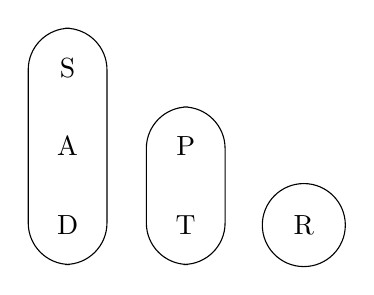
\begin{tikzpicture}[baseline={(S.base)}]
\node (S) at (0.5,2.5) {S};
\node (A) at (0.5,1.5) {A};
\node (D) at (0.5,0.5) {D};

\node (P) at (2.0,1.5) {P};
\node (T) at (2.0,0.5) {T};

\node (R) at (3.5,0.5) {R};

\draw [rounded corners=1.5em] (0.0,0.0) rectangle (1.0,3.0);
\draw [rounded corners=1.5em] (1.5,0.0) rectangle (2.5,2.0);
\draw (3.5,0.5) circle [radius=1.5em];
\end{tikzpicture}
\xe
\end{figure}

Essentially, Ayeri follows the same order of NPs\index{phrase types!noun phrase} as English in the construction
where the recipient\index{semantic role!recipient} appears as a prepositional phrase headed by \fw{to}.
However, the recipient\index{semantic role!recipient} is not an adjunct\index{grammatical function!adjunct}---it must be an argument. That is, it
is not possible to have multiple recipient\index{semantic role!recipient} NPs\index{phrase types!noun phrase} (unless one coordinates\index{coordination} them
with \xayr{nj}{nay}{and}), just as it is not possible to have multiple patients\index{semantic role!patient}
with transitive verbs\index{verbs!transitive}. Furthermore, it is not possible to link either the theme\index{semantic role!theme}
and the recipient\index{semantic role!recipient}, or the recipient\index{semantic role!recipient} and an adjunct\index{grammatical function!adjunct} with \xayr{nj}{nay}
{and}---only non-arguments can be coordinated\index{coordination} this way \citep[181]{carnie2013}.
Likewise, it is not possible for patient\index{semantic role!patient}, recipient\index{semantic role!recipient}, and adjuncts\index{grammatical function!adjunct} like 
\xayr{krFdNFy}{kardangya}{at school} in (\ref{ex:doubleobj}) to randomly switch
places with each other. Both the patient\index{semantic role!patient} and the recipient\index{semantic role!recipient} must be complements
of the verb together. The recipient\index{semantic role!recipient} is more readily expendable than the
theme\index{semantic role!theme}, however. Example (\ref{ex:doubleobjcstruct}) attempts to chart
this proposal as a c-structure tree.

\begin{figure}
\ex\label{ex:doubleobjcstruct}
\begin{forest} shorter edges, italic leaves
[IP
	[\anno{\xhead{I}}
		[{Ang ilya}, roof]
	]
	[\anno{S}
		[{\anno[\pass{\Top}]{NP}}
			[Apan]
		]
		[\anno{VP}
			[\anno{\xbar{V}}
				[{\anno[\pass{\Obj}]{NP}}
					[koyās]
				]
				[{\anno[\pass{\SObjc{recip}}]{NP}}
					[{yam Diya}, roof]
				]
			]
			[{\anno[\elem{\Adjc}]{NP}}
				[kardangya]
			]
		]
	]
]
\end{forest}
\xe
\end{figure}

\index{verbs!ditransitive|)}

\subsubsection{Control verbs}
\label{subsubsec:ctrlvb}
\index{verbs!control|(}

Control verbs have already been touched on in \autoref{subsec:control} in order
to compare Ayeri to Tagalog\index{Tagalog} in terms of syntactic alignment. In this section, I
want to elaborate on their structural and functional properties. Since \Lfg{}\index{Lexical-functional grammar}
does not assume empty nodes to carry semantic or functional value, there is no
\textsc{pro} element in c-structure trees here. VP complements of control verbs
are simply treated as \XCompl{}s,\index{grammatical function!open complement} that is, open complements\index{grammatical function!open complement}. These \XCompl{}s\index{grammatical function!open complement}
are dependent on the superordinate verb for the subject\index{grammatical function!subject} function: control verbs
share their semantic subject\index{grammatical function!subject} or object\index{grammatical function!primary object} with the semantic subject\index{grammatical function!subject} of a
(non-finite\index{verbs!non-finite}) subordinate verb \citep[289\psqq]{bresnan2016}.
% , also compare the English examples in (\ref{ex:engctrlstruct})
Typical S-control verbs in Ayeri are
\xayr{Ep/}{epa-}{refuse},
\xayr{liMk/}{linka-}{try},
\xayr{no/}{no-}{plan},\footnote{This is the same stem as the modal particle 
\rayr{no}{no}, but as the related content verb.}
\xayr{pebuk/}{pebuka-}{promise},
\xayr{sr/}{sara-}{go}, and
\xayr{vtYF/}{vac-}{like},\footnote{This verb also exists as a modal particle
\rayr{vtY}{vaca} with the same meaning.}
among others. On the other hand, typical O-control verbs are, for instance,
\xayr{glmF/}{galam-}{expect},
\xayr{kilisF/}{kilis-}{allow},
\xayr{nelF/}{nel-}{help},
\xayr{nos/}{nosa-}{order},
\xayr{pinY/}{pinya-}{ask}, and
\xayr{tonisF/}{tonis-}{convince}. Examples of the c- and f-structure of control
verbs in Ayeri are provided in (\ref{ex:ctrlstruct}).

Topicalization\index{grammatical function!topic} of NPs\index{phrase types!noun phrase} in subordinate VPs by matrix verbs is not possible in
Ayeri if the subordinate verb stands in between\index{word order} the matrix verb and the
subordinate verb's arguments. Thus, the \xayr{nyiNsF}{nayingas}{roof} in both
(\ref{ex:ctrlstruct}ab) cannot be the topic\index{grammatical function!topic} of the verb in the respective
matrix clauses, \xayr{liMky}{linkaya}{(he) tries} and
\xayr{nelFye}{nelye}{(she) helps}. Since topicalization\index{grammatical function!topic} does not apply to
non-finite verbs\index{verbs!non-finite}, the subordinate verb in both sentences,
\xayr{sidegYmF}{sidejam}{repairing}, cannot be marked for topic\index{grammatical function!topic} within its own
f-structure core either.

% \begin{figure}
% \pex\label{ex:engctrlstruct}
% \a%
% Subject control in English \citep[289]{bresnan2016}:\\

% \begin{minipage}[t]{.3\remaining}%\vspace{2\baselineskip}
% \begin{forest} shorter edges, italic leaves,
% [IP$_{f1}$
% 	[DP \tikzmark{engctrlstruct1_sus}
% 		[Susan]
% 	]
% 	[VP
% 		[V
% 			[kept]
% 		]
% 		[VP$_{f2}$ \tikzmark{engctrlstruct1_eat}
% 			[V
% 				[eating]
% 			]
% 			[DP \tikzmark{engctrlstruct1_mar}
% 				[marshmallows]
% 			]
% 		]
% 	]
% ]
% \end{forest}
% \end{minipage}
% \hfill
% \begin{avm}
% $f_1$: \[
% 	\Subj	&	\tikzmark{engctrlstruct1_subj} \[
% 		\avmspan{``Susan''} \\
% 	\] \tikzmark{engctrlstruct1_subj1} \\
% 	\Pred	&	\astruct{keep}{($f_1$ \Subj) ($f_1$ \XCompl)} \\
% 	\Tense	&	\Pst \\
% 	\XCompl	&	$f_2$: \tikzmark{engctrlstruct1_xcomp} \[
% 		\Subj	&	\tikzmark{engctrlstruct1_subj2} \\
% 		\Pred	&	\astruct{eat}{($f_2$ \Subj) ($f_2$ \Obj)} \\
% 		\Obj	&	\tikzmark{engctrlstruct1_obj} \[
% 			\avmspan{``marshmallows''} \\
% 		\] \\
% 	\] \\
% \]
% \end{avm}
% \begin{tikzpicture}[remember picture, overlay]
% \draw [-latex] ([yshift=1ex]{pic cs:engctrlstruct1_sus})
% 	to [out=east, in=west] ([yshift=1ex]{pic cs:engctrlstruct1_subj});
% \draw [-latex] ([yshift=1ex]{pic cs:engctrlstruct1_eat})
% 	to [out=east, in=west] ([yshift=1ex]{pic cs:engctrlstruct1_xcomp});
% \draw [-latex] ([yshift=1ex]{pic cs:engctrlstruct1_mar})
% 	to [out=east, in=west] ([yshift=1ex]{pic cs:engctrlstruct1_obj});
% \draw [rounded corners=1ex] ([yshift=1ex]{pic cs:engctrlstruct1_subj1})
% 	-- ++(east:7em) |- ([yshift=1ex]{pic cs:engctrlstruct1_subj2});
% \end{tikzpicture}

% \a%
% Object control in English \citep[292]{bresnan2016}:\\

% \begin{minipage}[t]{.3\remaining}\vspace{1\baselineskip}
% \begin{forest} for tree={s sep-=.5em,s=0}, shorter edges, italic leaves
% [IP$_{f1}$
% 	[DP \tikzmark{engctrlstruct2_sus}
% 		[Susan]
% 	]
% 	[VP
% 		[V
% 			[kept]
% 		]
% 		[DP \tikzmark{engctrlstruct2_joh}
% 			[John]
% 		]
% 		[VP$_{f2}$ \tikzmark{engctrlstruct2_dou}
% 			[V
% 				[doubting]
% 			]
% 			[DP \tikzmark{engctrlstruct2_him}
% 				[himself]
% 			]
% 		]
% 	]
% ]
% \end{forest}
% \end{minipage}
% \hfill
% \begin{avm}
% $f_1$: \[
% 	\Subj	&	\tikzmark{engctrlstruct2_subj} \[
% 		\avmspan{``Susan''} \\
% 	\] \\
% 	\Pred	&	\astruct{keep}{($f_1$ \Subj) ($f_1$ \Obj) ($f_1$ \XCompl)} \\
% 	\Tense	&	\Pst \\
% 	\Obj	&	\tikzmark{engctrlstruct2_obj} \[
% 		\avmspan{``John''} \\
% 	\] \tikzmark{engctrlstruct2_obj3} \\
% 	\XCompl	&	$f_2$: \tikzmark{engctrlstruct2_xcomp} \[
% 		\Subj	&	\tikzmark{engctrlstruct2_subj2} \\
% 		\Pred	&	\astruct{doubt}{($f_2$ \Subj) ($f_2$ \Obj)} \\
% 		\Obj	&	\tikzmark{engctrlstruct2_obj2} \[
% 			\avmspan{``himself''} \\
% 		\] \\
% 	\] \\
% \]
% \end{avm}
% \begin{tikzpicture}[remember picture, overlay]
% \draw [-latex] ([yshift=1ex]{pic cs:engctrlstruct2_sus})
% 	to [out=east, in=west] ([yshift=1ex]{pic cs:engctrlstruct2_subj});
% 	\draw [-latex] ([yshift=1ex]{pic cs:engctrlstruct2_joh})
% 	to [out=east, in=west] ([yshift=1ex]{pic cs:engctrlstruct2_obj});
% \draw [-latex] ([yshift=1ex]{pic cs:engctrlstruct2_dou})
% 	to [out=east, in=west] ([yshift=1ex]{pic cs:engctrlstruct2_xcomp});
% \draw [-latex] ([yshift=1ex]{pic cs:engctrlstruct2_him})
% 	to [out=east, in=west] ([yshift=1ex]{pic cs:engctrlstruct2_obj2});
% \draw [rounded corners=1ex] ([yshift=1ex]{pic cs:engctrlstruct2_obj3})
% 	-- ++(east:2em) |- ([yshift=1ex]{pic cs:engctrlstruct2_subj2});
% \end{tikzpicture}

% \xe
% \end{figure}

\begin{figure}
\pex\label{ex:ctrlstruct}
\a\label{ex:ctrlstruct_1}%
\begingl
	\glpreamble Subject control: //
	\gla Linkaya ang @ Mican sidejam nayingley. //
	\glb linka-ya ang= Mican sideg-yam naying-ley //
	\glc try-\TsgM{} \Aarg{}= Mican repair-\Ptcp{} roof-\PargI{} //
	\glft `Mican tries to repair the roof.' //
\endgl\medskip

\begin{minipage}[t]{.3\remaining}%\vspace{2\baselineskip}
\begin{forest} shorter edges, italic leaves,
[IP$_f$
	[\xhead{I}
		[Linkaya]
	]
	[S
		[NP \tikzmark{ctrlstruct1_mic}
			[{ang Mican}, roof]
		]
		[VP
			[VP$_g$ \tikzmark{ctrlstruct1_sid}
				[\xhead{V}
					[sidejam]
				]
				[NP \tikzmark{ctrlstruct1_nay}
					[nayingley]
				]
			]
		]
	]
]
\end{forest}
\end{minipage}
\hfill
\begin{avm}
$f$: \[
	\Pred	&	\astruct{try}{($f$ \Subj) ($f$ \XCompl)} \\
	\Subj	&	\tikzmark{ctrlstruct1_subj} \[
		\avmspan{``Mican''} \\
	\] \tikzmark{ctrlstruct1_subj1} \\
	\XCompl	&	$g:$ \tikzmark{ctrlstruct1_xcomp} \[
		\Pred	&	\astruct{repair}{($g$ \Subj) ($g$ \Obj)} \\
		\Subj	&	\tikzmark{ctrlstruct1_subj2} \\
		\Obj	&	\tikzmark{ctrlstruct1_obj} \[
			\avmspan{``roof''} \\
		\] \\
	\] \\
\]
\end{avm}
\begin{tikzpicture}[remember picture, overlay]
\draw [-latex] ([yshift=1ex]{pic cs:ctrlstruct1_mic})
	to [out=east, in=west] ([yshift=1ex]{pic cs:ctrlstruct1_subj});
\draw [-latex] ([yshift=1ex]{pic cs:ctrlstruct1_sid})
	to [out=east, in=south west] ([yshift=-1ex]{pic cs:ctrlstruct1_xcomp});
\draw [-latex] ([yshift=1ex]{pic cs:ctrlstruct1_nay})
	to [out=east, in=west] ([yshift=1ex]{pic cs:ctrlstruct1_obj});
\draw [rounded corners=1ex] ([yshift=1ex]{pic cs:ctrlstruct1_subj1})
	-- ++(east:11em) |- ([yshift=1ex]{pic cs:ctrlstruct1_subj2});
\end{tikzpicture}

\a\label{ex:ctrlstruct_2}%
\begingl
	\glpreamble Object control: //
	\gla Ang @ nelye {} @ Piha sa @ Mican sidejam nayingley. //
	\glb ang= nel-ye Ø= Piha sa= Mican sideg-yam naying-ley //
	\glc \AgtT{}= help-\TsgF{} \Top{}= Piha \Parg{}= Mican repair-\Ptcp{}
		roof-\PargI{} //
	\glft `Piha helps Mican repair the roof.' //
\endgl\medskip

\begin{minipage}[t]{.3\remaining}\vspace{3\baselineskip}
\begin{forest} shorter edges, italic leaves
[IP$_f$
	[\xhead{I}
		[{Ang nelye}, roof]
	]
	[S
		[NP \tikzmark{ctrlstruct2_pih}
			[Piha]
		]
		[VP
			[NP \tikzmark{ctrlstruct2_mic}
				[{sa Mican}, roof]
			]
			[VP$_g$ \tikzmark{ctrlstruct2_sid}
				[\xhead{V}
					[sidejam]
				]
				[NP \tikzmark{ctrlstruct2_nay}
					[nayingley]
				]
			]
		]
	]
]
\end{forest}
\end{minipage}
\hfill
\begin{avm}
$f$: \[
	\Pred	&	\astruct{help}{($f$ \Subj) ($f$ \Obj) ($f$ \XCompl)} \\
	\Top	&	\tikzmark{ctrlstruct2_top1} \[
		\avmspan{``Piha''} \\
	\] \tikzmark{ctrlstruct2_top2} \\
	\Subj	&	\tikzmark{ctrlstruct2_subj} \\
	\Obj	&	\tikzmark{ctrlstruct2_obj} \[
		\avmspan{``Mican''} \\
	\] \tikzmark{ctrlstruct2_obj3} \\
	\XCompl	&	$g:$ \tikzmark{ctrlstruct2_xcomp} \[
		\Pred	&	\astruct{repair}{($g$ \Subj) ($g$ \Obj)} \\
		\Subj	&	\tikzmark{ctrlstruct2_subj2} \\
		\Obj	&	\tikzmark{ctrlstruct2_obj2} \[
			\avmspan{``roof''} \\
		\] \\
	\] \\
\]
\end{avm}
\begin{tikzpicture}[remember picture, overlay]
\draw [-latex] ([yshift=1ex]{pic cs:ctrlstruct2_pih})
	to [out=east, in=west] ([yshift=1ex]{pic cs:ctrlstruct2_top1});
	\draw [-latex] ([yshift=1ex]{pic cs:ctrlstruct2_mic})
	to [out=east, in=west] ([yshift=1ex]{pic cs:ctrlstruct2_obj});
\draw [-latex] ([yshift=1ex]{pic cs:ctrlstruct2_sid})
	to [out=east, in=south west] ([yshift=-1ex]{pic cs:ctrlstruct2_xcomp});
\draw [-latex] ([yshift=1ex]{pic cs:ctrlstruct2_nay})
	to [out=east, in=west] ([yshift=1ex]{pic cs:ctrlstruct2_obj2});

\draw [rounded corners=1ex] ([yshift=1ex]{pic cs:ctrlstruct2_top2})
	-- ++(east:1em) |- ([yshift=1ex]{pic cs:ctrlstruct2_subj});
\draw [rounded corners=1ex] ([yshift=1ex]{pic cs:ctrlstruct2_obj3})
	-- ++(east:11em) |- ([yshift=1ex]{pic cs:ctrlstruct2_subj2});
\end{tikzpicture}

\xe
\end{figure}

Furthermore, the process which places the matrix verb in \xhead{I} seems to be
applicable as well to the subordinate verb if this leads to no doubling of
semantic roles in the linear order of constituents in the clause. That is,
there must not be two patient\index{semantic role!patient} arguments after the verb, even if they are part
of different f-structures. This means that fronting\index{word order} the verb as possibly a
complement of \xhead{I} in order to be able to topicalize\index{grammatical function!topic} NPs\index{phrase types!noun phrase} subcategorized by
the subordinate verb in (\ref{ex:ctrlstruct_1}) is possible, while it is not in
(\ref{ex:ctrlstruct_2}). Example (\ref{ex:ctrlinc}) subsequently illustrates
the raising\index{verbs!raising} of a subordinate verb. The topic\index{grammatical function!topic} particle, as usual, appears as a
proclitic\index{clitics} before the verb, which here encodes an inanimate patient\index{semantic role!patient} topic\index{grammatical function!topic},
referring to an argument of the subordinate verb, \xayr{nyiNF}{naying}{roof}.
In order to adress the \Top{} function of the matrix verb in this case, we have
to use inside-out functional uncertainty and annotate the topicalized\index{grammatical function!topic} NP\index{phrase types!noun phrase} with
\uncertain{\XCompl}{\Top}~=~↓ to signal that \Top{} is an attribute of the
f-structure containing \XCompl{}\index{grammatical function!open complement}. This is an extension to the rules stated in
(\ref{ex:topmorphlex}).

\begin{figure}
\ex\label{ex:ctrlinc}
\begingl
	\gla Le @ linkaya sidejam ang @ Mican naying. //
	\glb le= linka-ya sideg-yam ang= Mican naying-Ø //
	\glc \PargI{}= try-\TsgM{} repair-\Ptcp{} \Aarg{}= Mican roof-\Top{} //
	\glft `The roof, Mican tries to repair it.' //
\endgl\medskip

\begin{minipage}[t]{.45\remaining}
\begin{forest} shorter edges, italic leaves, for tree={s sep-=2em,s=0},
[IP
	[\anno{\xbar{I}}
			[\anno{\xhead{I}}
				[{Le linkaya}, roof]
			]
		[{\anno[\pass{\XCompl}]{VP}}
			[sidejam]
		]
	]
	[\anno{S}
		[{\anno[\pass{\Subj}]{NP}}
			[{ang Mican}, roof]
		]
		[\anno{VP}
			[{\anno[\pass{\XCompl}]{VP}}
				[{\anno[\uncertain{\XCompl}{\Top}~=~↓]{NP}}
					[naying]
				]
			]
		]
	]
]
\end{forest}%\medskip
\end{minipage}
~
\begin{avm}
\[
	\Pred	&	\astruct{try}{\ups{\Subj} \ups{\XCompl}} \\
	
	\Top	&	\[
			\avmspan{``roof''} \\
	\] \tikzmark{ctrlinc_top} \\

	\Subj	&	\[
		\avmspan{``Mican''} \\
	\] \tikzmark{ctrlinc_subj1} \\
	
	\XCompl	&	\[
		\Pred	&	\astruct{repair}{\ups{\Subj} \ups{\Obj}} \\
		\Subj	&	\tikzmark{ctrlinc_subj2} \\
		\Obj	&	\tikzmark{ctrlinc_obj} \\
	\] \\
\]
\end{avm}
\begin{tikzpicture}[remember picture, overlay]
\draw [rounded corners=1ex] ([yshift=1ex]{pic cs:ctrlinc_top})
	-- ++(east:11.5em) |- ([yshift=1ex]{pic cs:ctrlinc_obj});
\draw [rounded corners=1ex] ([yshift=1ex]{pic cs:ctrlinc_subj1})
	-- ++(east:10.25em) |- ([yshift=1ex]{pic cs:ctrlinc_subj2});
\end{tikzpicture}
\xe
\end{figure}

\index{verbs!control|)}

\subsubsection{Raising verbs}
\label{subsubsec:raisvb}
\index{verbs!raising|(}

Raising verbs, like control verbs\index{verbs!control}, are verbs which take a VP complement whose
subject\index{grammatical function!subject} is shared with the subject\index{grammatical function!subject} or the object\index{grammatical function!primary object} of the matrix verb. They as
well have already been dealt with briefly in \autoref{subsec:raising} with
regards to questions of syntactic alignment. In contrast to control verbs\index{verbs!control}, the
syntactic subject\index{grammatical function!subject} of the matrix verb is not semantically an argument of it, but
of the subordinate verb. The subject\index{grammatical function!subject} of the matrix verb may thus also be a
dummy \fw{it} or \fw{there} in English. Ayeri seems to only have
\xayr{surFpF/}{surp-}{seem} as a raising verb.\footnote{This is likely an
artefact of working mostly in English, since \fw{seem} is a very common verb
there. Since it is interesting for Ayeri to have only one verb which works this
way, apparently, I decided to leave it in for now. Alternatively, it would be a
reasonable next step in grammaticalization for the verb to turn into a modal\index{modals}
particle, \rayr{surFp} {surpa}. The dictionary also lists
\xayr{kFr/}{kra-}{tend} with no further comment, entered on
\DTMdate{2005-11-22}, and possibly intended to be used as a raising verb
meaning `have a tendency' rather than `look after, care for'. There is also
\xayr{rmYF/}{ramy-}{let, let go of} which was intended as a raising causative
verb and which was entered early on as well (\DTMdate{2006-05-24}). Ayeri can
express causative relationships by case marking, though (see
\autoref{subsubsec:valincr}). If need be, \rayr{rmYF/} {ramy-} can be used with
a complement clause\index{complement clause} instead of a verbal complement.} Instead of using verbal
expressions like \fw{happen}, \fw{tend}, and \fw{be likely}, one may rather use
adverbials or adverbs\index{adverbs} like \xayr{mmNeri}{mamangeri}{by coincidence},
\xayr{kFraaneri}{krāneri}{by tendency} and \xayr{nilj}{nilay} {probably}.
English has raising verbs like \fw{expect}, \fw{order}, or \fw{want}, which may
take an object\index{grammatical function!primary object} and a verbal complement, but whose syntactic object\index{grammatical function!primary object} is the
semantic subject\index{grammatical function!subject} of the subordinate verb. Ayeri, however, lacks the
raising-to-object\index{verbs!ECM@\textsc{ecm}} mechanism and instead requires a complement clause\index{complement clause}.

\begin{figure}
\pex\label{ex:raisestruct}
\a\label{ex:raisestruct_1}\begingl
	\glpreamble Raising to subject: //
	\gla Surpya ang @ Ajān valyyam umangley. //
	\glb surp-ya ang= Ajān valy-yam umang-ley //
	\glc seem-\TsgM{} \Aarg{}= Ajān enjoy-\Ptcp{} beach-\PargI{} //
	\glft `Ajān seems to enjoy the beach.' //
\endgl\medskip

\begin{minipage}[t]{.3\remaining}
\begin{forest} shorter edges, italic leaves,
[IP$_f$
	[\xhead{I}
		[Surpya]
	]
	[S
		[NP \tikzmark{raisestruct1_aja}
			[{ang Ajān}, roof]
		]
		[VP
			[VP$_g$ \tikzmark{raisestruct1_val}
				[\xhead{V}
					[valyyam]
				]
				[NP \tikzmark{raisestruct1_uma}
					[umangley]
				]
			]
		]
	]
]
\end{forest}
\end{minipage}
\hfill
\begin{avm}
$f$: \[
	\Pred	&	\astruct[($f$ \Subj)]{seem}{($f$ \XCompl)} \\

	\Subj	&	\tikzmark{raisestruct1_subj1} \[
		\avmspan{``Ajān''} \\
	\] \tikzmark{raisestruct1_subj2} \\

	\XCompl	&	$g$: \tikzmark{raisestruct1_xcomp} \[
		\Pred	&	\astruct{enjoy}{($g$ \Subj) ($g$ \Obj)} \\
		\Subj	&	\tikzmark{raisestruct1_subj3} \\
		\Obj	&	\tikzmark{raisestruct1_obj} \[
			\avmspan{``beach''} \\
		\] \\
	\] \\
\]
\end{avm}
\begin{tikzpicture}[remember picture, overlay]
\draw [-latex] ([yshift=1ex]{pic cs:raisestruct1_aja})
	to [out=east, in=west] ([yshift=1ex]{pic cs:raisestruct1_subj1});
\draw [-latex] ([yshift=1ex]{pic cs:raisestruct1_val})
	to [out=east, in=south west] ([yshift=-1ex]{pic cs:raisestruct1_xcomp});
\draw [-latex] ([yshift=1ex]{pic cs:raisestruct1_uma})
	to [out=east, in=west] ([yshift=1ex]{pic cs:raisestruct1_obj});
\draw [rounded corners=1ex] ([yshift=1ex]{pic cs:raisestruct1_subj2})
	-- ++(east:11em) |- ([yshift=1ex]{pic cs:raisestruct1_subj3});
\end{tikzpicture}

\a\label{ex:raisestruct_2}\begingl
	\glpreamble Raising to object: //
	\gla \textup{\ljudge*} @ Ang @ paronye {} @ Niva sa @ Ajān valyyam
		umangley. //
	\glb {} ang= paron-ye Ø= Niva sa= Ajān valy-yam umang-ley //
	\glc {} \AgtT{}= believe-\TsgF{} \Top{}= Niva \Parg{}= Ajān enjoy-\Ptcp{}
		beach-\PargI{} //
	\glft \textit{Intended:} `Niva believes Ajān to enjoy the beach.' //
\endgl\medskip

\begin{minipage}[t]{.3\remaining}\vspace{4\baselineskip}
\begin{forest} shorter edges, italic leaves,
[IP$_f$
	[\xhead{I}
		[{Ang paronye}, roof]
	]
	[S
		[NP \tikzmark{raisestruct2_niv}
			[Niva]
		]
		[VP
			[NP \tikzmark{raisestruct2_aja}
				[{sa Ajān}, roof]
			]
			[VP$_g$ \tikzmark{raisestruct2_val}
				[\xhead{V}
					[valyyam]
				]
				[NP \tikzmark{raisestruct2_uma}
					[umangley]
				]
			]
		]
	]
]
\end{forest}
\end{minipage}
\hfill
\begin{avm}
$f$: \[
	\Pred	&	\astruct[($f$ \Obj)]{believe}{($f$ \Subj) ($f$ \XCompl)} \\

	\Top	&	\tikzmark{raisestruct2_top1} \[
		\avmspan{``Niva''} \\
	\] \tikzmark{raisestruct2_top2} \\

	\Subj	&	\tikzmark{raisestruct2_subj1} \\

	\Obj	&	\tikzmark{raisestruct2_obj1} \[
		\avmspan{``Ajān''} \\
	\] \tikzmark{raisestruct2_obj2} \\

	\XCompl	&	$g$: \tikzmark{raisestruct2_xcomp} \[
		\Pred	&	\astruct{enjoy}{($g$ \Subj) ($g$ \Obj)} \\
		\Subj	&	\tikzmark{raisestruct2_subj2} \\
		\Obj	&	\tikzmark{raisestruct2_obj3} \[
			\avmspan{``beach''} \\
		\] \\
	\] \\
\]
\end{avm}
\begin{tikzpicture}[remember picture, overlay]
\draw [-latex] ([yshift=1ex]{pic cs:raisestruct2_niv})
	to [out=east, in=west] ([yshift=1ex]{pic cs:raisestruct2_top1});
\draw [-latex] ([yshift=1ex]{pic cs:raisestruct2_aja})
	to [out=east, in=west] ([yshift=1ex]{pic cs:raisestruct2_obj1});
\draw [-latex] ([yshift=1ex]{pic cs:raisestruct2_val})
	to [out=east, in=south west] ([yshift=-1ex]{pic cs:raisestruct2_xcomp});
\draw [-latex] ([yshift=1ex]{pic cs:raisestruct2_uma})
	to [out=east, in=west] ([yshift=1ex]{pic cs:raisestruct2_obj3});

\draw [rounded corners=1ex] ([yshift=1ex]{pic cs:raisestruct2_top2})
	-- ++(east:1em) |- ([yshift=1ex]{pic cs:raisestruct2_subj1});
\draw [rounded corners=1ex] ([yshift=1ex]{pic cs:raisestruct2_obj2})
	-- ++(east:11em) |- ([yshift=1ex]{pic cs:raisestruct2_subj2});
\end{tikzpicture}

\xe
\end{figure}

Superficially, the charts in (\ref{ex:raisestruct}) look more or less identical
to those in (\ref{ex:ctrlstruct}). However, while the a-structure definitions
in the matrix verbs' \Pred{} feature in (\ref{ex:ctrlstruct}) define their
subjects\index{grammatical function!subject} and objects\index{grammatical function!primary object} as arguments, the verbs in (\ref{ex:raisestruct}) do not.
Instead, (\ref{ex:raisestruct_1}) defines only an \XCompl{}\index{grammatical function!open complement} as an argument, and
its \Subj{} is defined as an athematic subject\index{grammatical function!subject} \citep[304--308]{bresnan2016}.
This is indicated by placing the function label outside of the pointed
brackets. The same goes for the \Obj{} in (\ref{ex:raisestruct_2}): here as
well, the object\index{grammatical function!primary object} is not strictly an argument of the matrix verb. In the
accompanying \Avm{}s, the respective athematic functions in $f$ are connected
to the \Subj{} function in $g$ in both cases to indicate coherence.

The example sentence in (\ref{ex:raisestruct_2}) is also marked ungrammatical
in contrast to the previous example, (\ref{ex:ctrlstruct_2}). Even though both
sentences may be structurally similar in their constituency, their matrix verbs
differ in argument structure:

\pex\label{ex:ctrlraisecomp}
\a\label{ex:ctrlraisecomp_octrl}%
	\astruct{help}{\ups{\Subj} \ups{\Obj} \ups{\XCompl}}

\a\label{ex:ctrlraisecomp_raiseo}%
	\astruct[\ups{\Obj}]{believe}{\ups{\Subj} \ups{\XCompl}}
\xe

While \fw{help} subcategorizes for a thematic object\index{grammatical function!primary object}, \fw{believe} does not.
Its syntactic object\index{grammatical function!primary object} is not actually its semantic object\index{grammatical function!primary object} here: the status of
\fw{someone} in \fw{believe someone} is different from that in
\fw{believe someone to do something}. Apparently, Ayeri is able to unify a
thematic object\index{grammatical function!primary object} with the subject\index{grammatical function!subject} of a subordinate verb, in spite of
discrepancies in case\index{case} marking between agent\index{case!agent} and patient\index{case!patient}. On the other hand, an
athematic object\index{grammatical function!primary object} cannot be unified with the subject\index{grammatical function!subject} of a subordinate verb.
% A thematic object can thus become a subordinate thematic subject, but an
% athematic object cannot become a subordinate thematic subject.
Hence, Ayeri allows \xayr{nelF/}{nel-}{help} to be an object\index{grammatical function!primary object}-control verb\index{verbs!control}, but
it does not allow \xayr{pronF/}{paron-}{believe} to be a raising-to-object\index{verbs!ECM@\textsc{ecm}}
verb. Note again, however, that even raising-to-subject is only common in Ayeri
with \xayr{surFpF/}{surp-}{seem}, so Ayeri more generally seems to have an
aversion towards raising. Or, assuming that the difference to English is
lexical, Ayeri's verbs do not allow for athematic functions with the notable
exception of \rayr{surFpF/}{surp-}. Instead of an \XCompl{}\index{grammatical function!open complement} and an athematic
function, they subcategorize for a \Compl{}\index{grammatical function!closed complement}.

\begin{figure}
\ex\label{ex:raiseinc}
\begingl
	\gla Le @ surpya valyyam ang @ Ajān umang. //
	\glb le= surp-ya valy-yam ang= Ajān umang-ley //
	\glc \PatTI{}= seem-\TsgM{} enjoy-\Ptcp{} \Aarg{}= Ajān beach-\Top{} //
	\glft `The beach, Ajān seems to enjoy it.' //
\endgl\medskip

\begin{minipage}[t]{.45\remaining}
\begin{forest} shorter edges, italic leaves, for tree={s sep-=1.75em,s=0},
[IP
	[\anno{\xbar{I}}
			[\anno{\xhead{I}}
				[{Le surpya}, roof]
			]
		[{\anno[\pass{\XCompl}]{VP}}
			[valyyam]
		]
	]
	[\anno{S}
		[{\anno[\pass{\Subj}]{NP}}
			[{ang Ajān}, roof]
		]
		[\anno{VP}
			[{\anno[\pass{\XCompl}]{VP}}
				[{\anno[\uncertain{\XCompl}{\Top}~=~↓]{NP}}
					[umang]
				]
			]
		]
	]
]
\end{forest}%\medskip
\end{minipage}
~
\begin{avm}
\[
	\Pred	&	\astruct[\ups{\Subj}]{seem}{\ups{\XCompl}} \\
	
	\Top	&	\[
			\avmspan{``beach''} \\
	\] \tikzmark{raiseinc_top} \\

	\Subj	&	\[
		\avmspan{``Ajān''} \\
	\] \tikzmark{raiseinc_subj1} \\
	
	\XCompl	&	\[
		\Pred	&	\astruct{enjoy}{\ups{\Subj} \ups{\Obj}} \\
		\Subj	&	\tikzmark{raiseinc_subj2} \\
		\Obj	&	\tikzmark{raiseinc_obj} \\
	\] \\
\]
\end{avm}
\begin{tikzpicture}[remember picture, overlay]
\draw [rounded corners=1ex] ([yshift=1ex]{pic cs:raiseinc_top})
	-- ++(east:11em) |- ([yshift=1ex]{pic cs:raiseinc_obj});
\draw [rounded corners=1ex] ([yshift=1ex]{pic cs:raiseinc_subj1})
	-- ++(east:10.5em) |- ([yshift=1ex]{pic cs:raiseinc_subj2});
\end{tikzpicture}
\xe
\end{figure}

Just as with control verbs\index{verbs!control}, it is possible to front\index{word order} the subordinate verb,
effectively generating it as a complement of the matrix verb in \xhead{I}
according to the working hypothesis already used for control verbs\index{verbs!control}. This way as
well, it is possible to topicalize\index{grammatical function!topic} arguments of the subordinate verb, the
condition being that no argument functions are doubled here as well. Again, the
subordinate verb and the VP with its dependent NPs\index{phrase types!noun phrase} both have to be annotated
\pass{\XCompl}, and the topicalized\index{grammatical function!topic} NP\index{phrase types!noun phrase} has to be marked with
\uncertain{\XCompl}{\Top}~=~↓ in accordance with the position of the topic\index{grammatical function!topic}
marker as adjoined to the left edge of the matrix verb's f-structure. Again,
the subordinate verb is non-finite\index{verbs!non-finite} and thus cannot carry topic\index{grammatical function!topic} marking.

An example of this is given in (\ref{ex:raiseinc}). Here, the VP which would
normally carry the subordinate \xhead{V}, \xayr{vlYFymF}{valyyam}{enjoying}, is
headless, just as the VP which would normally contain \xhead{I},
\xayr{le surFpFy}{le surpya}{(he) seems}. The subordinate verb is instead found
as a sister node to the matrix verb. However, both verbs' complements are
generated in their usual position: the VP complementing the matrix verb is a
daughter of the VP sister of the subject NP\index{phrase types!noun phrase}, \rayr{ANF AgYaanF}{ang Ajān}. This
VP, in turn, has an NP\index{phrase types!noun phrase} complement carrying the object of the subordinate verb,
\xayr{UmNF}{umang}{beach}. The subordinate VP is discontinuous here as well, so
both parts are marked \XCompl{}\index{grammatical function!open complement}. The subordinate verb's object is also the
topic\index{grammatical function!topic} which the matrix verb is marked for by \rayr{le}{le}. In order to place
the \Top{} function at the correct f-structure level, inside-out functional
uncertainty is used to indicate that \rayr{UmNF}{umang} feeds into the \Top{}
function of the superior f-structure which specifies \XCompl{}\index{grammatical function!open complement}.

\index{verbs!raising|)}

\subsubsection{Expletive \emph{sitang}}
\label{subsec:expsitang}

It has been mentioned before that \xayr{sitNF}{sitang}{self} can also be used
as an expletive pronoun in such a way that quantifiers\index{quantifiers} can be attributed to
subject\index{grammatical function!subject} pronouns which are realized as pronominal clitics\index{clitics}, compare 
\autoref{subsec:reflrec} and \autoref{subsec:quantfloat}. The quantifier\index{quantifiers} cannot
follow\index{word order} the pronominal clitic\index{clitics} directly due to the double function of many
quantifiers\index{quantifiers} as intensifiers\index{intensifiers} which modify the verb. Ayeri otherwise uses the
demonstratives\index{pronouns!demonstrative} \xayr{AdnY}{adanya}{that one} or \xayr{dnY}{danya}{(such) one}
as dummy pronouns, but these encode a third-person\index{person} reference (see
\autoref{subsubsec:demprosyn}, p.~\pageref{subsubsec:demprosyn}). As 
(\ref{ex:expsitang}) shows, it is also possible, however, to quantify personal
pronouns\index{pronouns!personal} of persons\index{person} other than the third. Thus, \rayr{sitNF}{sitang} is used in
this context as a dummy pronoun since ordinarily, it does not encode person\index{person},
but reflexivity. It is hence neutral to person\index{person} features while still
establishing an anaphoric relationship to its binder. It also gives the clitic\index{clitics}
something to lean on which is not the verb or an adverb.

\begin{figure}
\begin{minipage}[t]{.67\remaining}
\ex\label{ex:expsitang}\begingl
	\gla Le @ cānnang sitang-ikan kondan. //
	\glb le= cān=nang sitang=ikan kondan-Ø //
	\glc \PatTI{}= love=\Fpl{}.\Aarg{} self=many food-\Top{} //
	\glft `Food, many of us love it.' //
\endgl\medskip

\begin{forest} shorter edges, italic leaves,
[IP
	[\xhead{I} % \anno{\xhead{I}}
		[\xhead{I} % \anno{\xhead{I}}
			[{Le cān}, roof]
		]
		[Cl \tikzmark{expsitang_nan} % \anno{Cl}
			[-nang$_i$]
		]
	]
	[S % \anno{S}
		[DP\tikzmark{expsitang_DP} \tikzmark{expsitang_sit}
			% {\anno[\pass{\Subj}]DP}
			[\xhead{D} % \anno{\xhead{D}}
				[\xhead{D} % \anno{\xhead{D}}
					[sitang$_i$]
				]
				[Cl \tikzmark{expsitang_ika} % {\anno[\elem{\Adjc}]{Cl}}
					[-ikan]
				]
			]
		]
		[NP % {\anno[\pass{\Obj}]{NP}}
			[\xhead{N} % \anno{\xhead{N}}
				[kondan]
			]
		]
	]
]
\end{forest}
\xe
\end{minipage}
\hfill
{\smaller%
\begin{avm}
\[
	\Pred	&	\astruct{love}{\ups{\Subj} \ups{\Obj}} \\

	\Subj	&	\tikzmark{expsitang_subj} \[
		\Pred	&	`$pro$' \\
		\Pers	&	\First \\
		\Num	&	\Pl \\
		\Case	&	\Aarg \\
		\Anim	&	$+$ \\

		\Quant	&	\tikzmark{expsitang_qnt} \[
			\Pred	&	`many' \\
		\] \\
	\] \\

	... \\
\]
\end{avm}}
\begin{tikzpicture}[remember picture, overlay]
\draw [-latex] ([yshift=1ex]{pic cs:expsitang_nan})
	to [out=east, in=west] ([yshift=1ex]{pic cs:expsitang_subj});
\draw [-latex] ([yshift=1ex]{pic cs:expsitang_sit})
	to [out=east, in=west] ([yshift=1ex]{pic cs:expsitang_subj});
\draw [-latex] ([yshift=1ex]{pic cs:expsitang_ika})
	to [out=east, in=west] ([yshift=1ex]{pic cs:expsitang_qnt});
\end{tikzpicture}
\end{figure}

In spite of \rayr{sitNF}{sitang} being used as a reflexivizing prefix\index{prefixes}
otherwise, it has not been analyzed as adding [\Refl{}~$+$] to the
\Subj{} function in (\ref{ex:expsitang}). This is because of its use as a dummy
here; essentially, it adds no meaning besides establishing an anaphoric
relationship which is marked in the example as an index $i$. Since it cannot be
declined either, all person\index{person} features rest in the pronominal clitic\index{clitics}, \xayr{/nNF}
{nang}{we}. Distributed exponence maps both the pronominal clitic's\index{clitics} semantic
content and that of the subject\index{grammatical function!subject} DP\index{phrase types!determiner phrase}, \rayr{sitNF/IknF}{sitang-ikan}, onto the
\Subj{} function in the partial f-structure diagram. The only lexical content
which the subject\index{grammatical function!subject} DP\index{phrase types!determiner phrase} contains is that of the quantifier\index{quantifiers} clitic\index{clitics},
\xayr{/IknF}{-ikan}{many}. Since this information is quantifying in nature, it
feeds into the \Quant{} list of the \Subj{} function to create a unified
meaning of `many of us' in spite of the parts which create this meaning being
scattered over \xhead{I} and the subject\index{grammatical function!subject} DP\index{phrase types!determiner phrase}.

Going by classic, structuralist binding theory, \rayr{sitNF}{sitang} should be
able to bind the subject\index{grammatical function!subject} clitic\index{clitics} because \rayr{tYaanFnNF}{cānnang} as a unit
c-commands \rayr{sitNF/IknF}{sitang-ikan}, among others. In terms of \Lfg{}'s
functionally oriented binding theory, both the subject\index{grammatical function!subject} pronoun and
\rayr{sitNF/IknF}{sitang-ikan} are part of the same f-structure core created by
the predicator \xayr{tYaanF/}{cān-}{love}, and the binder f-precedes the
bindee. Thus, it is possible to establish an anaphoric relationship between
them.

\subsection{Existential statements}
\label{subsec:exs}

While Ayeri uses a zero copula\index{copula}, there are nonetheless full verbs expressing
existence: \xayr{yom/}{yoma-}{be (in a place), exist}, as well as the
comparison\index{comparison} verbs\index{verbs!comparative} \xayr{km/}{kama-}{be as} \xayr{ENF/}{eng-}{be more} and
\xayr{v/}{va-}{be most}. Obviously, the comparison\index{comparison} verbs are related to the
enclitic\index{clitics} suffixes\index{suffixes} described in \autoref{subsec:adjcomp}. By extension, the verb
meaning `give', \rayr{IlF/}{il-}, can also be used to mean `be less'.
Theoretically, there is also \xayr{verY/}{varya-}{be least},\footnote{From
\xayr{v/}{va-}{be most} + \rayr{/ArY}{-arya} (categorial negation\index{negation}).} but that
has never seen much practical use, and neither has \rayr{IlF/}{il-} in its
negative comparative meaning.

In order to express \fw{there is}, Ayeri uses \rayr{yom/}{yoma-} with a dummy
subject\index{grammatical function!subject} pronoun: \xayr{yomreNF}{yomareng}{there is/are}, which is a set
expression---literally, `it exists'. That is, \rayr{yomreNF}{yomareng} is even
used with plural\index{number!plural} complements, and can be inflected for the usual morphological
features of verbs, as shown in (\ref{ex:yomareng}), where the verb carries
negation\index{negation},
that is, it frequently comes with a locative\index{case!locative} complement to express that someone
or something exists in relation to a place. Less formally, however, a copulaic\index{copula}
construction may as well be used for these purposes, compare the examples in
(\ref{ex:yomaplace}). The copular-clause\index{copular clause} strategy comes at the slight
disadvantage of not being able to use verb morphology.

\begin{figure}
\pex\label{ex:yomareng}
\a\label{ex:yomareng_sg}\begingl
	\gla Le @ yomoyreng kanga-ma bibanjyam siku. //
	\glb le= yoma-oy=reng kanga-Ø=ma biban-ye-yam siku //
	\glc \PatTI{}= be-\Neg{}=\TsgI{}.\Aarg{} milk-\Top{}=enough
		cake-\Pl{}-\Dat {} pan //
	\glft `There is not enough milk for pancakes.' //
\endgl

\a\label{ex:yomareng_pl}\begingl
	\gla Le @ yomareng nārya hemaye-ma. //
	\glb le= yoma=reng nārya hema-ye-Ø=ma //
	\glc \PatTI{}= be=\TsgI{}.\Aarg{} though egg-\Pl{}-\Top{}=enough //
	\glft `There are enough eggs, though.' //
\endgl
\xe
\end{figure}

\begin{figure}
\pex\label{ex:yomaplace}
\a\label{ex:yomaplace_1}
\begin{minipage}[t]{.5\remaining}
\begingl
	\gla Ang @ yomasaya {} @ Mican visamya. //
	\glb ang= yoma-asa-ya Ø= Mican visam-ya //
	\glc \AgtT{}= be-\Hab{}-\TsgM{} \Top{}= Mican capital-\Loc{} //
	\glft `Mican is usually in the capital.' //
\endgl
\end{minipage}
\hfill
\begin{avm}
\[
	\Pred	&	\astruct{be}{\ups{\Subj} \ups{\Oblq{loc}}} \\
	\Asp	&	\Hab \\

	\Top	&	\[
		\avmspan{``Mican''} \\
	\] \tikzmark{yomaplace1_top} \\
	
	\Subj	&	\tikzmark{yomaplace1_subj} \\
	
	\Oblq{loc}	&	\[
		\Pred	&	`capital' \\
		\Case	&	\Loc \\
	\]
\]
\end{avm}
\begin{tikzpicture}[remember picture, overlay]
\draw [rounded corners=1ex] ([yshift=1ex]{pic cs:yomaplace1_top})
	-- ++(east:1em) |- ([yshift=1ex]{pic cs:yomaplace1_subj});
\end{tikzpicture}

\a\label{ex:yomaplace_2}
\begin{minipage}[t]{.25\remaining}
\begingl
	\gla Yāng sangalya. //
	\glb Yāng sangal-ya //
	\glc \TsgM{}.\Aarg{} room-\Loc{} //
	\glft `He's in the room.' //
\endgl
\end{minipage}
\hfill
\begin{avm}
\[
	\Pred	&	\astruct{null-be}{\ups{\Subj} \ups{\Plink}} \\

	\Subj	&	\[
		\avmspan{``he''} \\
	\] \\

	\Plink	&	\[
		\Pred	&	`room' \\
		\Case	&	\Loc \\
	\] \\
\]
\end{avm}

\xe
\end{figure}

An alternative to the comparison\index{comparison} strategy by enclitics\index{clitics} is to use a verb of
comparison\index{comparison}\index{verbs!comparative} as listed initially. Ayeri behaves differently in this from what
\citet{wals121} reports on the way `exceed comparatives' work, however.
According to him,

\blockcquote{wals121}{Exceed Comparatives have as their characteristic that the
standard NP\index{phrase types!noun phrase} is constructed as the direct object of a transitive verb with the
meaning \enquote{to exceed} or \enquote{to surpass}. Thus, the construction
typically includes two predicates, one which is the comparative predicate, and
another which is the \enquote{exceed}-verb.}

Also compare \citet{beermannetal2005}. What is described by \citet{wals121} has
similarities to a serial-verb construction, as shown in (\ref{ex:svcexceed}).

\ex\label{ex:svcexceed}
	\textsc{comparee} is \textsc{quality} exceeds \textsc{standard}
\xe

Ayeri does not possess serial-verb constructions, however. Instead, it
superficially appears as though comparative verbs take the quality adjective\index{adjectives} as
a modifier, essentially in the way of an adverb. Nonetheless, the subject\index{grammatical function!subject} forms
the comparee, and the object\index{grammatical function!primary object} the standard. An example is given in
(\ref{ex:ayrexceed}). More generally, the structure in Ayeri is as stated in
(\ref{ex:ayrexceedscheme}).

\begin{figure}[h]
\ex\label{ex:ayrexceed}\begingl
	\gla Eng @ engaran nake rivanye vana danyaley nana. //
	\glb eng= eng-aran nake rivan-ye-Ø vana danya-ley nana //
	\glc \AgtTI{}= be.more-\TplI{} tall mountain-\Pl{}-\Top{} \Second{}.\Gen{}
		one-\PargI{} \Fpl{}.\Gen{} //
	\glft `Your mountains are higher than ours.' //
\endgl
\xe
\end{figure}

\begin{figure}[h]
\ex~\label{ex:ayrexceedscheme}%
	exceeds \textsc{quality} \textsc{comparee} \textsc{standard}
\xe
\end{figure}

The way \Lfg{}\index{Lexical-functional grammar} handles comparison\index{comparison} of adjectives\index{adjectives} in predicative\index{grammatical function!predicative complement} contexts is
sketched out in \citet[122]{butt1999}, see (\ref{ex:lfgpredcomp}). As expected,
the predicative\index{grammatical function!predicative complement} complement is contained within a \Plink{}\index{grammatical function!predicative complement} function. Comparison\index{comparison}
morphology is represented through functional annotations, \Deg{} and \Degdim{},
to express \fw{more than} as a positive comparative in this case; \fw{-er than}
would receive the same annotation because it is functionally equivalent. The
adjective\index{adjectives} itself is analyzed as subcategorizing for a complement which holds
the standard of comparison\index{comparison}.

\begin{figure}[h]
\ex\label{ex:lfgpredcomp}%
English \parencite[adapted from][122]{butt1999}: \medskip

\fw{It is more comfortable than a tractor.}\medskip

\begin{avm}
\[
	\Pred	&	\astruct{be}{\ups{\Subj} \ups{\Plink}} \\

	\Subj	&	\[
		\avmspan{``it''} \\
	\] \\

	\Plink	&	\[
		\Pred	&	\astruct{comfortable}{\ups{\Compl}} \\
		\Deg	&	\Comp \\
		\Degdim	&	$positive$ \\

		\Compl	&	\[
			\avmspan{``tractor''} \\
		\] \\
	\] \\
\]
\end{avm}
\xe
\end{figure}

Since the functional analysis of \Lfg{}\index{Lexical-functional grammar} is intended to be as independent of the
morphology of individual languages as possible, how can we analyze Ayeri in
this regard, especially since the verbs encode \Deg{} and \Degdim{}, and the
adjective\index{adjectives} seems to appear in the place an adverb\index{adverbs} would normally inhabit? In
fact, the \Avm{} in (\ref{ex:lfgpredcomp}) has a certain similarity to those
presented for control\index{verbs!control} and raising verbs\index{verbs!raising}, compare (\ref{ex:ctrlstruct}) and
(\ref{ex:raisestruct}). In all cases, there is a subordinate predicator
subcategorizing for a complement. What if rather than treating the quality in
the way of an adverb, Ayeri actually generalized the way subordinate verbs can
be fronted\index{word order}, treating the adjective\index{adjectives} in the way of a verbal complement of
\xhead{I}? This hypothesis neatly coincides with Ayeri's strategy of fronting\index{word order}
subordinate verbs in order to enable topicalization of their dependents by
making the embedded NPs\index{phrase types!noun phrase} look like regular arguments of the matrix clause's
verb.

First of all, example (\ref{ex:vcompmorphlex}) gives the morpholexical
annotations for all comparative verbs,\index{verbs!comparative} \xayr{km/}{kama-}{be as},
\xayr{ENF/}{eng-}{be more}, \xayr{v/}{va-}{be most}, \xayr{IlF/}{il-}{be less},
and \xayr{verY/}{varya-}{be least}. Only the definitions extending those in
(\ref{ex:inflmorphlex}) are listed, however. Here, the verb contains
information on the comparison\index{comparison} status of the predicative\index{grammatical function!predicative complement} complement as well as
about its polarity: the table contains all possible permutations for the values
of \ups{\Plink{} \Deg{}} and \ups{\Plink{} \Degdim{}}.\index{grammatical function!predicative complement}

\begin{figure}
\begin{morphlex}
\pex\label{ex:vcompmorphlex}%
\a\adjustbox{valign=t}{%
	\begin{tabu} {\usetabu{morphlex}}
	\rayr{\larger km/}{kama-}
		& I
		& \begin{tabu}[t]{@{} l @{ } l @{ } X[l]}
			\ups{\Pred} & = & \astruct{be-as}{\ups{\Subj} \ups{\Plink}} \\
			\ups{\Plink} & = & ↓ \\
				\quad\downs{\Deg} & = & \Pos \\
				\quad\downs{\Degdim} & = & $equative$ \\
		\end{tabu}
	\end{tabu}%
}

\a\adjustbox{valign=t}{%
	\begin{tabu} {\usetabu{morphlex}}
	\rayr{\larger ENF/}{eng-}
		& I
		& \begin{tabu}[t]{@{} l @{ } l @{ } X[l]}
			\ups{\Pred} & = & \astruct{be-more}{\ups{\Subj} \ups{\Plink}} \\
			\ups{\Plink} & = & ↓ \\
				\quad\downs{\Deg} & = & \Comp \\
				\quad\downs{\Degdim} & = & $positive$ \\
		\end{tabu}
	\end{tabu}%
}

\a\adjustbox{valign=t}{%
	\begin{tabu} {\usetabu{morphlex}}
	\rayr{\larger v/}{va-}
		& I
		& \begin{tabu}[t]{@{} l @{ } l @{ } X[l]}
			\ups{\Pred} & = & \astruct{be-most}{\ups{\Subj} \ups{\Plink}} \\
			\ups{\Plink} & = & ↓ \\
				\quad\downs{\Deg} & = & \Supl \\
				\quad\downs{\Degdim} & = & $positive$ \\
		\end{tabu}
	\end{tabu}%
}

\a\adjustbox{valign=t}{%
	\begin{tabu} {\usetabu{morphlex}}
	\rayr{\larger IlF/}{il-}
		& I
		& \begin{tabu}[t]{@{} l @{ } l @{ } X[l]}
			\ups{\Pred} & = & \astruct{be-less}{\ups{\Subj} \ups{\Plink}} \\
			\ups{\Plink} & = & ↓ \\
				\quad\downs{\Deg} & = & \Comp \\
				\quad\downs{\Degdim} & = & $negative$ \\
		\end{tabu}
	\end{tabu}%
}

\a\adjustbox{valign=t}{%
	\begin{tabu} {\usetabu{morphlex}}
	\rayr{\larger verY/}{varya-}
		& I
		& \begin{tabu}[t]{@{} l @{ } l @{ } X[l]}
			\ups{\Pred} & = & \astruct{be-least}{\ups{\Subj} \ups{\Plink}} \\
			\ups{\Plink} & = & ↓ \\
				\quad\downs{\Deg} & = & \Supl \\
				\quad\downs{\Degdim} & = & $negative$ \\
		\end{tabu}
	\end{tabu}%
}
\xe
\end{morphlex}
\end{figure}

Following the hypothesis above, the c-structure of a comparative statement in
Ayeri should look like in (\ref{ex:compcstruct}). This is purposefully designed
in parallel to (\ref{ex:ctrlinc}), even though the subject\index{grammatical function!subject} of the comparative
verb is not shared by the a-structure of the adjective\index{adjectives}. As in
(\ref{ex:ctrlinc}) and (\ref{ex:raiseinc}), the complement of the verb is
understood as a discontinuous constituent of the \Plink{}\index{grammatical function!predicative complement} type. The complement
of the adjective\index{adjectives} is generated in its canonical position\index{word order} as a daughter of the AP\index{phrase types!adjective phrase}
in S\index{phrase types!small clause}. Alternatively, it should be possible for the \xhead{A} not to be fronted,
just as the subordinate verb in (\ref{ex:ctrlstruct}) and
(\ref{ex:raisestruct}) appears as the head of the subordinate VP. However, this
leads to ambiguity in that an adjective\index{adjectives}, then, directly follows\index{word order} a noun, so
modification relationships would not be entirely clear. The preferred way is,
thus, to generate the adjective\index{adjectives} as a complement of \xhead{I}.

\begin{figure}
\ex\label{ex:compcstruct}\begingl
	\gla Ang @ engye para {} @ Cisu sa @ Kaman. //
	\glb ang= eng-ye para Ø= Cisu sa= Kaman //
	\glc \AgtT{}= be.more-\TsgF{} fast \Top{}= Cisu \Parg{}= Kaman //
	\glft `Cisu is faster than Kaman.' //
\endgl\medskip

\begin{minipage}[t]{.45\remaining}
%\vspace{1\baselineskip}
\lapbox[\width]{-\exoffset}{%
\begin{forest} shorter edges, italic leaves, for tree={s sep-=1.5em,s=0}
[IP
	[\anno{\xbar{I}}
		[\anno{\xhead{I}}
			[{Ang engye}, roof]
		]
		[{\anno[\pass{\Plink}]{AP}}% \tikzmark{compcstruct_par}
			[para]
		]
	]
	[\anno{S}
		[{\anno[\pass{\Subj}]{NP}}% \tikzmark{compcstruct_cis}
			[Cisu]
		]
		[\anno{VP}
			[{\anno[\pass{\Plink}]{AP}}% \tikzmark{compcstruct_ap}
				[{\anno[\pass{\Compl}]{NP}}% \tikzmark{compcstruct_kam}
					[{sa Kaman}, roof]
				]
			]
		]
	]
]
\end{forest}}
\end{minipage}
\hfill
\begin{avm}
\[
	\Pred	&	\astruct{be-more}{\ups{\Subj} \ups{\Plink}} \\

	\Top	&	\[%\tikzmark{compcstruct_top1} \[
		\avmspan{``Cisu''}
	\] \tikzmark{compcstruct_top2} \\

	\Subj	&	\tikzmark{compcstruct_subj} \\

	\Plink	&	\[%\tikzmark{compcstruct_plink} \[
		\Pred	&	\astruct{fast}{\ups{\Compl}} \\
		\Deg	&	\Comp \\
		\Degdim	&	$positive$ \\
		\Compl	&	\[%\tikzmark{compcstruct_compl} \[
			\avmspan{``Kaman''}	\\
		\] \\
	\] \\
\]
\end{avm}
\begin{tikzpicture}[remember picture, overlay]
% \draw [-latex] ([yshift=1ex]{pic cs:compcstruct_cis})
% 	to [out=east, in=west] ([yshift=1ex]{pic cs:compcstruct_top1});
% \draw [-latex] ([yshift=1ex]{pic cs:compcstruct_par})
% 	to [out=east, in=west] ([yshift=1ex]{pic cs:compcstruct_plink});
% \draw [-latex] ([yshift=1ex]{pic cs:compcstruct_ap})
% 	to [out=east, in=west] ([yshift=1ex]{pic cs:compcstruct_plink});
% \draw [-latex] ([yshift=1ex]{pic cs:compcstruct_kam})
% 	to [out=east, in=west] ([yshift=1ex]{pic cs:compcstruct_compl});
% 
\draw [rounded corners=1ex] ([yshift=1ex]{pic cs:compcstruct_top2})
	-- ++(east:1em) |- ([yshift=1ex]{pic cs:compcstruct_subj});
\end{tikzpicture}

\xe
\end{figure}

In order to form clauses of the kind \fw{John is a better doctor than Bill},
with the quality composed of an NP\index{phrase types!noun phrase}--AP\index{phrase types!adjective phrase} combination, it is necessary to use a
relative clause\index{relative clause}: \fw{John is a doctor who is better than Bill}. Ayeri only
allows for \xhead{A} to be fronted\index{word order} if it does not modify a predicative\index{grammatical function!predicative complement} nominal.
The sentence in (\ref{ex:comppredn_1}) is thus ungrammatical because \xayr{bnF}{ban}{good} modifies a predicative\index{grammatical function!predicative complement} noun,
\xayr{kromyaasF}{karomayās}{doctor}. Since the adjective\index{adjectives} itself has a
complement, \rayr{s hiro}{sa Hiro}, there are two successive patient\index{semantic role!patient} arguments, 
which is not permissible. Example (\ref{ex:comppredn_2}), on the
other hand, shows the grammatical solution. Here, the
term under comparison\index{comparison}, being a \xayr{kromyaasF}{karomayās}{doctor}, is
constructed as a copular clause\index{copular clause} while the comparison\index{comparison} in quality between
\rayr{ApitYnF}{Apican} and \rayr{hiro}{Hiro} is moved into the relative clause\index{relative clause}.

\begin{figure}
\pex\label{ex:comppredn}
\a\label{ex:comppredn_1}\ljudge*%
\begin{minipage}[t]{.5\remaining}
\begingl
	\gla Engya ban ang @ Apican karomayās sa @ Hiro. //
	\glb eng-ya ban ang= Apican karomaya-as sa= Hiro //
	\glc be.more-\TsgM{} good \Aarg{}= Apican doctor-\Parg{} \Parg{}= Hiro //
	\glft \textit{Intended:} `Apican is a better doctor than Hiro.' //
\endgl
\end{minipage}
\hfill
\begin{forest} shorter edges, italic leaves,
[IP
	[\xbar{I}, narrower nodes,
		[\xhead{I}
			[Engya]
		]
		[AP
			[ban]
		]
	]
	[S
		[NP
			[{ang Apican}, roof]
		]
		[VP
			[NP, narrower nodes,
				[\xhead{N}
					[karomayās]
				]
				[AP
					[NP
						[{sa Hiro}, roof]
					]
				]
			]
		]
	]
]
\end{forest}

\a\label{ex:comppredn_2}%
\begin{minipage}[t]{.5\remaining}
\begingl
	\gla Ang @ Apican karomayās si ang @ engya ban sa @ Hiro. //
	\glb ang= Apican karomaya-as si ang= eng-ya.Ø ban sa= Hiro //
	\glc \Aarg{}= Apican doctor-\Parg{} \Rel{} \AgtT{}= be.more=\TsgM{}.\Top{}
		good \Parg{}= Hiro //
	\glft `Apican is a doctor who is better than Hiro.' //
\endgl
\end{minipage}
\hfill
\begin{forest} shorter edges, italic leaves,
[S
	[{\anno[\pass{\Subj}]{NP}}
		[{Ang Apican}, roof]
	]
	[{\anno[\pass{\Plink}]{NP}}
		[\anno{\xhead{N}}
			[karomayās]
		]
		[{\anno[\elem{\Adjc}]{CP}}
			[{si ang engya ...}, roof]
		]
	]
]
\end{forest}

\xe
\end{figure}

\subsection{Secondary Predicates}
\label{subsec:secpred}

\hyperref[subsec:eqs]{Section~\ref*{subsec:eqs}} has only dealt with
predicative adjectives and nominals over the subject in order to illustrate a
very common basic type of statement. There are also secondary predicates,
however, which can be subdivided further into depictive and resultative
secondary predicates. A depictive\index{adjectives!depictive} secondary predicate, on the one hand,
\textcquote[173]{mueller2002}{provides information about the state of the
entity it refers to. This state holds at the time of the event described by the
verb}. A resultative\index{adjectives!resultative} secondary predicate, on the other hand, refers to
\textcquote[173]{mueller2002}{the result of an event [...]\ specified by the
adjective\index{adjectives}}. This difference is illustrated in (\ref{ex:engsecpred}).

\begin{figure}[h]
\pex\label{ex:engsecpred}
\a\label{ex:engsecpred1_subj}%
	\fw{Suzy came to work \textbf{sick}.}

\a\label{ex:engsecpred1_obj}%
	\fw{Jack eats the apple \textbf{unwashed}.}

\a\label{ex:engsecpred2_obj}%
	\fw{Bill wipes the table \textbf{clean}.}
\xe
\end{figure}

In (\ref{ex:engsecpred1_subj}), \fw{sick} does not describe the manner in which
Suzy came to work, but the state in which she did so. Similarly,
\fw{unwashed} in (\ref{ex:engsecpred1_obj}) refers to the state of the apple at
the time of being eaten rather than the manner in which it is eaten. It is also
possible to interpret the adjective as referring to Jack, but let us assume
that, in the context of this statement, it is rather more relevant for the
apple to be clean. In contrast to these two examples, \fw{clean} in
(\ref{ex:engsecpred2_obj}) does not refer to the state of the subject or the
object at the moment of wiping, but the state of the table as a result of being
wiped.

Unfortunately, \citet[347]{bresnan2016}, while mentioning resultatives, do not
go into detail about an \Lfg{} analysis of them, and do not say anything at all
about depictives. Though they give a few references about \Lfg{}-based surveys
of resultatives in English, a cursory web search does not bring up papers on
depictive predicates in terms of \Lfg{}. One has to assume that this topic
probably constitutes a desideratum\index{desiderata} at the time of writing.
\citet{dalrymple2001} does not touch the topic of secondary predication at all,
and neither do \citet{butt1999}; \citet{falk2001} only provides an analysis of
resultatives. As far as \Lfg{} analyses of resultatives go, \citet{simpson1983}
and \citet{christie2013} were used to inform the below discussion.
\textcites{mueller2002} provides analyses of both depictives and resultatives
in terms of constraint-based grammar, however, he does so from the point of
view of Head-driven Phrase-Structure Grammar (\textsc{hpsg};
\cite{pollardsag1994}) and uses only German as his object of study.
Nonetheless, his analyses informed the below discussion of depictives.

\subsubsection{Depictives}
\label{subsubsec:depict}
\index{adjectives!depictive|(}

English examples of depictive adjectives were given in (\ref{ex:engsecpred}ab).
Moreover, NPs\index{phrase types!noun phrase} can also be depictive predicates in English, for instance in 
\fw{John came out of the exam a nervous wreck}, where \fw{a nervous wreck}
describes the state of John as he returns from the exam. According to
\citet{mueller2002}'s analysis, \textcquote[196]{mueller2002}{the subject\index{grammatical function!subject} of
the depictive secondary predicate is coindexed with an element of the argument
structure of the primary predicate}. He suggests for \textsc{hpsg} \textquote{a
lexical rule that recategorizes predicative adjectives and prepositions so that
they can modify verbal elements} as a way to
\textcquote[196]{mueller2002}{capture the adjunct\index{grammatical function!adjunct} properties of depictive
secondary predicates}. I tried to cast this in (\ref{ex:depictfstruct}) as an
f-structure in which the depictive secondary predicate is an adjunct\index{grammatical function!adjunct} of the
verb. The anaphoric relationship between \Subj{} and the adjective is expressed
by $i$ as an index which marks that they are co-indexed.
% \footnote{Alternatively, one could maybe construct this as an f-structure
% embedded as an adjunct of the main verb. In this f-structure, the adjective
% would be a \Plink{} complement of a \fw{null-be} predicate whose subject is
% shared with an argument of the sentence's main verb. This would essentially
% result in a subject-control relationship, except that the subordinate
% f-structure is an adjunct to rather than an argument of the matrix verb.}

\begin{figure}
\ex\label{ex:depictfstruct}%
English:\medskip

\fw{Suzy$_i$ came to work sick$_i$.} \medskip

% \label{ex:depictfstruct_1}
% \begin{avm}
% \[
% 	\Pred	&	\astruct{come}{\ups{\Subj} \ups{\Oblq{to}}} \\
% 	\Tense	&	\Pst \\
% 	\Subj	&	\[
% 		\avmspan{``Suzy''} \\
% 	\] \tikzmark{depictfstruct1_ctrl} \\
% 	\Oblq{to}	&	\[
% 		\Pred	&	\astruct{to}{\ups{\Obj}} \\
% 		\PCase	&	$to$ \\
% 		\Obj	&	\[
% 			\avmspan{``work''} \\
% 		\] \\
% 	\] \\
% 	\Adjc	&	\{
% 		\[
% 			\Pred	&	\astruct{null-be}{\ups{\Subj} \ups{\Plink}} \\
% 			\Subj	&	\tikzmark{depictfstruct1_subj} \\
% 			\Plink	&	\[
% 				\avmspan{``sick''} \\
% 			\] \\
% 		\] \\
% 	\} \\
% \]
% \end{avm}
% \begin{tikzpicture}[remember picture, overlay]
% \draw [rounded corners=1ex] ([yshift=1ex]{pic cs:depictfstruct1_ctrl})
% 	-- ++(east:17em) |- ([yshift=1ex]{pic cs:depictfstruct1_subj});
% \end{tikzpicture}
%
% \label{ex:depictfstruct_2}
\begin{avm}
\[
	\Pred	&	\astruct{come}{\ups{\Subj} \ups{\Oblq{to}}} \\
	\Tense	&	\Pst \\
	\Subj	&	\[
		\avmspan{``Suzy$_i$''} \\
	\] \\
	\Oblq{to}	&	\[
		\Pred	&	\astruct{to}{\ups{\Obj}} \\
		\PCase	&	$to$ \\
		\Obj	&	\[
			\avmspan{``work''} \\
		\] \\
	\] \\
	\Adjc	&	\{
		\[
			\Pred	&	`sick$_i$' \\
		\] \\
	\} \\
\]
\end{avm}

\xe
\end{figure}

In Ayeri, the depictive adjective, whether it refers to the subject\index{grammatical function!subject} or the
object\index{grammatical function!primary object}, follows\index{word order} the verb. This nicely fits the analysis fashioned after
\citet{mueller2002} above, by which the depictive acts as an adjunct\index{grammatical function!adjunct} of the
verb with reference to one of the verb's arguments. Ayeri makes no formal
distinction between adjectives and adverbs, but context should clarify under
normal circumstances. An example of depictive secondary predicates in Ayeri is
given in (\ref{ex:depict}). In (\ref{ex:depict_subj}), there is only a subject\index{grammatical function!subject},
\rayr{gd}{Gada} to be described by the adjective, \xayr{pisu}{pisu}{tired}. In
(\ref{ex:depict_obj}), the adjective, \xayr{tuvo}{tuvo}{red} (here in the
meaning `raw') can describe either the subject\index{grammatical function!subject} or the object\index{grammatical function!primary object}, but semantically,
it makes most sense for it to refer to the object\index{grammatical function!primary object}, \xayr{InunF}{inun}{fish}. It
may be noted again here that topicalization has no impact on the argument of
the verb the secondary predicate refers to (compare 
\autoref{subsec:secpredctrl}).

\begin{figure}
\pex\label{ex:depict}
\a\label{ex:depict_subj}
\begin{minipage}[t]{.45\remaining}
\begingl
	\gla Radanye pisu ang @ Gada. //
	\glb radan-ye pisu ang= Gada //
	\glc wake.up-\TsgF{} tired \Aarg{}= Gada //
	\glft `Gada wakes up tired.' //
\endgl\medskip

\begin{avm}
\[
	\Pred	&	\astruct{wake-up}{\ups{\Subj}} \\
	\Subj	&	\[
		\avmspan{``Gada$_i$''} \\
	\] \\
	\Adjc	&	\{\[
		\Pred	&	`tired$_i$' \\
	\]\} \\
\]
\end{avm}
\end{minipage}
\hfill
\begin{forest} shorter edges, italic leaves,
[IP
	[\anno{\xbar{I}}
		[\anno{\xhead{I}}
			[Radanye]
		]
		[{\anno[\elem{\Adjc}]{AP}}
			[pisu]
		]
	]
	[\anno{S}
		[{\anno[\pass{\Subj}]{NP}}
			[{ang Gada}, roof]
		]
	]
]
\end{forest}

\a\label{ex:depict_obj}
\begin{minipage}[t]{.45\remaining}
\begingl
	\gla Le @ konja tuvo ang @ Kaji inun. //
	\glb le= kond-ya tuvo ang= Kaji inun //
	\glc \PatTI{}= eat-\TsgM{} raw \Aarg{}= Kaji fish-\Top{} //
	\glft `The fish, Kaji eats it raw.' //
\endgl\medskip

\begin{avm}
\[
	\Pred	&	\astruct{eat}{\ups{\Subj} \ups{\Obj}} \\
	\Top	&	\[
		\avmspan{``fish$_i$''} \\
	\] \tikzmark{depictobj_top} \\
	\Subj	&	\[
		\avmspan{``Kaji''} \\
	\] \\
	\Obj	&	\tikzmark{depictobj_obj} \\
	\Adjc	&	\{\[
		\Pred	&	`raw$_i$' \\
	\]\} \\
\]
\end{avm}
\begin{tikzpicture}[remember picture, overlay]
\draw [rounded corners=1ex] ([yshift=1ex]{pic cs:depictobj_top})
	-- ++(east:1em) |- ([yshift=1ex]{pic cs:depictobj_obj});
\end{tikzpicture}
\end{minipage}
\hfill
\begin{forest} shorter edges, narrower nodes, italic leaves,
[IP
	[\anno{\xbar{I}}
		[\anno{\xhead{I}}
			[{Le konja}, roof]
		]
		[{\anno[\elem{\Adjc}]{AP}}
			[tuvo]
		]
	]
	[\anno{S}
		[{\anno[\pass{\Subj}]{NP}}
			[{ang Kaji}, roof]
		]
		[\anno{VP}
			[{\anno[\pass{\Obj}]{NP}}
				[inun]
			]
		]
	]
]
\end{forest}

\xe
\end{figure}

As mentioned initially, there is also the possibility of nominal depictives.
These are introduced with the proclitic\index{clitics} expressing likeness, \rayr{ku/}{ku-}.
Since secondary complements are adjuncts\index{grammatical function!adjunct}, they are not subcategorized for by
the verb, so the question is which case they should receive---Ayeri, curiously,
does not assign case\index{case} to these NPs\index{phrase types!noun phrase}.\footnote{One might be tempted to analyze
\rayr{ku/}{ku-} as a case\index{case} marker used for essive and equative functions.
NPs\index{phrase types!noun phrase} marked with \rayr{ku/}{ku-} may be regularly case-marked\index{case} in other contexts,
though, and Ayeri does not make use of multiple case\index{case} marking or
\fw{suffixaufnahme} otherwise. Moreover, there is none of the usual alternation
between overtly marked and zero-marked forms with \rayr{ku/}{ku-}. The
distribution of \rayr{ku/}{ku-} is thus different from that of typical case\index{case}
markers.} Nominal depictives may appear right after\index{word order} the verb or as adjuncts\index{grammatical function!adjunct} of
the VP if they are heavy. This is illustrated in (\ref{ex:nomdepict}): while
the NP\index{phrase types!noun phrase} \xayr{ku/sikty}{ku-sikataya}{as a winner} follows the verb directly in
(\ref{ex:nomdepict_1}), the depictive NP\index{phrase types!noun phrase} \xayr{ku/ArilinY—kovro}{ku-arilinya
... kovaro}{someone ... easily} in (\ref{ex:nomdepict_2}) is trailing at the
end of the phrase as a result of being modified by a relative clause\index{relative clause}.

\begin{figure}
\pex\label{ex:nomdepict}
\a\label{ex:nomdepict_1}
\begin{minipage}[t]{.45\remaining}
\begingl
	\gla Sa-sahaya ku-sikataya ang @ Mahān. //
	\glb sa\til{}saha-ya ku=sikataya ang= Mahān //
	\glc \Iter{}\til{}come-\TsgM{} as=winner \Aarg{}= Mahān //
	\glft `Mahān returned (as) a winner.' //
\endgl \medskip

\begin{avm}
\[
	\Pred	&	\astruct{come}{\ups{\Subj}} \\
	\Asp	&	\Iter \\
	\Subj	&	\[
		\avmspan{``Mahān$_i$''} \\
	\] \\
	\Adjc	&	\{\[
		\Pred	&	`winner$_i$' \\
	\]\}
\]
\end{avm}
\end{minipage}
~
\begin{forest} shorter edges, narrower nodes, italic leaves,
[IP
	[\anno{\xbar{I}}
		[\anno{\xhead{I}}
			[Sa-sahaya]
		]
		[{\anno[\elem{\Adjc}]{NP}}
			[ku-sikataya]
		]
	]
	[\anno{S}
		[{\anno[\pass{\Subj}]{NP}}
			[{ang Mahān}, roof]
		]
	]
]
\end{forest}

\a\label{ex:nomdepict_2}
\begin{minipage}[t]{.45\remaining}
\begingl
	\gla Nakasye ang @ Apitu ku-arilinya si tesisoyyes kovaro. //
	\glb nakas-ye ang= Apitu ku=arilinya si tesisa-oy=yes kovaro //
	\glc grow.up-\TsgF{} \Aarg{}= Apitu as=someone \Rel{} 
		betray-\Neg{}=\TsgF{}.\Aarg{} easily //
	\glft `Apitu grew up someone not betrayed easily.' //
\endgl \medskip

\begin{avm}
\[
	\Pred	&	\astruct{grow-up}{\ups{\Subj}} \\
	\Subj	&	\[
		\avmspan{``Apitu$_i$''}
	\] \\
	\Adjc	&	\{\[
		\avmspan{\normalfont ``someone$_i$ not ...''} \\
	\]\}
\]
\end{avm}
\end{minipage}
~
\begin{forest} shorter edges, narrower nodes, italic leaves,
[IP
	[\anno{\xhead{I}}
		[Nakasye]
	]
	[\anno{S}
		[{\anno[\pass{\Subj}]{NP}}
			[{ang Apitu}, roof]
		]
		[\anno{VP}
			[{\anno[\elem{\Adjc}]{DP}}
				[\anno{\xhead{D}}
					[ku-arilinya]
				]
				[{\anno[\elem{\Adjc}]{CP}}
					[{si tesisoyyes kovaro}, roof]
				]
			]
		]
	]
]
\end{forest}

\xe
\end{figure}

\index{adjectives!depictive|)}

\subsubsection{Resultatives}
\label{subsubsec:res}
\index{adjectives!resultative|(}

\citet{simpson1983} comes to the conlusion that resultatives always modify
objects\index{grammatical function!primary object}, whether they are surface objects\index{grammatical function!primary object} or `underlying objects\index{grammatical function!primary object}' (like the
subjects\index{grammatical function!subject} of passives\index{voice!passive} or of verbs like \fw{shatter} when used intransitively).
Furthermore, according to her, verbs may be analyzed as being subcategorized
for resultatives in analogy to control\index{verbs!control} and raising verbs\index{verbs!raising}. She proposes, thus,
that there is a lexical rule which adds an \XCompl{}\index{grammatical function!open complement} to a verb's
subcategorization frame whose subject\index{grammatical function!subject} is the verb's logical object\index{grammatical function!primary object}. This
observation is squared with the argument structure of verbs in terms of the
semantic role of the subject\index{grammatical function!subject} function: according to \citet{perlmutter1978},
intransitive verbs\index{verbs!intransitive} can be grouped into unergative\index{verbs!unergative} and unaccusative\index{verbs!unaccusative} depending on
whether their syntactic subject\index{grammatical function!subject} is also their logical subject\index{grammatical function!subject}, or their logical
object\index{grammatical function!primary object}, compare (\ref{ex:verbtyp}).\footnote{The terms \citet{perlmutter1978}
introduces, however, appear to be not completely unproblematic today. As
\citet{dixon2010b} writes, \textcquote[156]{dixon2010b}{the labels
\enquote{unaccusative} and \enquote{unergative} are used for such a wide
variety of phenomena as to be essentially imprecise and unclear. [...]\ Their
employment provides the false sense of a universal semantic basis for varied
grammatical properties. They are best avoided}. In the literature consulted as
a theoretical background for this section, `unaccusative' and `unergative' are
used in their basic definition as provided by \citet{perlmutter1978} and
summarized in (\ref{ex:verbtyp}), and I will stick to this definition here as
well. Also compare \citet[334--336]{bresnan2016}.} \citet{mueller2002} seems to
argue along similar lines, but from an \textsc{hpsg} perspective.

\begin{figure}
\pex\label{ex:verbtyp}%
Syntactic typology of intransitive verbs\index{verbs!intransitive}
\parencites{perlmutter1978}{bresnan2016}:
\a \begin{minipage}[t]{\remaining}
	unergative
	\begin{itemize}[leftmargin=*]
		\item S\tsub{A} with [–\,o] $\mapsto$ S
		\item S typically in control of the action
		\item \fw{\textbf{He} ran}
	\end{itemize}
	\end{minipage}

\a \begin{minipage}[t]{\remaining}
	unaccusative
	\begin{itemize}[leftmargin=*]
		\item S\tsub{P} with [–\,r] $\mapsto$ S
		\item S typically not in control of the action
		\item \fw{\textbf{The tree} fell}
	\end{itemize}
	\end{minipage}
\xe
\end{figure}

In English, a variety of phrase types can form resultative secondary
predicates: APs\index{phrase types!adjective phrase}, NPs\index{phrase types!noun phrase}, and PPs\index{phrase types!prepositional phrase} \parencites{simpson1983}{christie2013}. While
English (like other Germanic languages) makes heavy use of intransitive
prepositions as constituent parts of verbs such as \fw{knock out}, \fw{lock
in}, or \fw{look over}, this is not so in Ayeri (compare \autoref{manga},
p.~\pageref{manga}). Examples with transitive\index{verbs!transitive} adpositions where the PP\index{phrase types!prepositional phrase} is not
an adjunct\index{grammatical function!adjunct} should also be hard to find. An example for each phrase type
complementing the object\index{grammatical function!primary object} of a transitive verb\index{verbs!transitive} to express a result is given in
(\ref{ex:restrns}). The sentence in (\ref{ex:restrns_pp2}) is adapted from
\citet{christie2013}, and here the status of the PP\index{phrase types!prepositional phrase} as an argument of the verb
is not entirely clear, probably because of the added-argument status of
\XCompl{}s\index{grammatical function!open complement} which she asserts. It may also be pointed out that in 
(\ref{ex:restrns_np}) we can see another use of the dative\index{case!dative}, that is, to mark
resultative NPs\index{phrase types!noun phrase}. A verb may thus occur exceptionally with more than one
complement in the dative case\index{case!dative}. However, different from a regular recipient\index{semantic role!recipient} or
a goal\index{semantic role!goal} NP\index{phrase types!noun phrase}, a resultative dative\index{case!dative} NP\index{phrase types!noun phrase} also normally occurs after\index{word order} the verb.

\begin{figure}
\pex\label{ex:restrns}
\a\label{ex:restrns_ap}%
	\begingl
		\glpreamble object\index{grammatical function!primary object} NP\index{phrase types!noun phrase} + resultative AP\index{phrase types!adjective phrase}: //
		\gla Ang @ gondaya \textbf{apitu} {} @ Sedan prihinley. //
		\glb ang= gonda-ya apitu Ø= Sedan prihin-ley //
		\glc \AgtT{}= wipe-\TsgM{} clean \Top{}= Sedan table-\PargI{} //
		\glft `Sedan wipes the table clean.' //
	\endgl

\a\label{ex:restrns_np}%
	\begingl
		\glpreamble object\index{grammatical function!primary object} NP\index{phrase types!noun phrase} + resultative NP\index{phrase types!noun phrase}: //
		\gla Ang @ visya \textbf{nernanjyam} \textbf{kivo} {} @ Amān
			seygoley. //
		\glb ang= vis-ya nernan-ye-yam kivo Ø= Amān seygo-ley //
		\glc \AgtT{}= cut-\TsgM{} piece-\Pl{}-\Dat{} small \Top{}= Amān 
			apple-\PargI{} //
		\glft `Amān cuts the apple into little pieces.' //
	\endgl

\a\label{ex:restrns_pp1}%
	\begingl
		\glpreamble object\index{grammatical function!primary object} NP\index{phrase types!noun phrase} + resultative PP\index{phrase types!prepositional phrase} (intransitive\index{verbs!intransitive}): //
		\gla Ang @ tapyye \textbf{miday} {} @ Briha tovaley. //
		\glb ang= tapy-ye miday Ø= Briha tova-ley //
		\glc \AgtT{}= put-\TsgF{} around \Top{}= Briha tova-ley //
		\glft `Briha puts a cloak on.' //
	\endgl

\a\label{ex:restrns_pp2}%
	\begingl
		\glpreamble object\index{grammatical function!primary object} NP\index{phrase types!noun phrase} + resultative PP\index{phrase types!prepositional phrase} (transitive\index{verbs!transitive}): //
		\gla Ang @ hiyaye {} @ Gada suranley \textbf{avan} 
			\textbf{turayyam}. //
		\glb ang= hiya-ye Ø= Gada suran-ley avan turay-yam //
		\glc \AgtT{}= roll-\TsgF{} \Top{}= Gada ball-\PargI{} bottom
			hill-\Dat{} //
		\glft `Gada rolls a ball down the hill.' //
	\endgl

\xe
\end{figure}

As with other secondary predicates, the normal place for a resultative to appear
in is behind the verb, unless the complement is syntactically heavy and in this
position makes the connection between the verb and its subject\index{grammatical function!subject} hard to grasp,
as is the case with \xayr{AvnF turjymF}{avan turayyam}{down the hill} in
(\ref{ex:restrns_pp2}): compared to the other examples in (\ref{ex:restrns}),
this phrase consists of two words and contains its own complement. While
(\ref{ex:restrns_np}) also contains a modifier and likewise consists of two
words, the modifier is not an argument but an adjunct\index{grammatical function!adjunct}. The NP\index{phrase types!noun phrase} with an adjective
is thus relatively more light than the PP\index{phrase types!prepositional phrase} still.

According to \citet{simpson1983}, the structure all of the examples in
(\ref{ex:restrns}) have in common is something along the lines of what is
illustrated by (\ref{ex:restrnsstr}). This, however, is an interpretation which
extrapolates from the article because she only gives the a-structure
definition, but no f- and c-structures. \citet{simpson1983} explicitly likens
the a-structure of transitive\index{verbs!transitive} clauses with unergative verbs\index{verbs!unergative} to that of
control verbs\index{verbs!control}---she analyzes resultative secondary predicates in terms of
functional control by interpreting the object\index{grammatical function!primary object} of the verb as the subject\index{grammatical function!subject} of the
resultative.

My interpretation is that this suggests a structure as described for copular
clauses\index{copular clause} (\autoref{subsec:eqs}), so there should be a \fw{null-be} predicator
requiring a subject\index{grammatical function!subject} and a predicative\index{grammatical function!predicative complement} complement as its arguments here as
well---the head of the \XCompl{}\index{grammatical function!open complement} is basically the construction itself here as
well. This f-structure $g$ forms an open complement\index{grammatical function!open complement} of the verb in $f$. The
\XCompl{}\index{grammatical function!open complement} as a phrase has no equivalent in the form of a maximal projection in
the c-structure tree in (\ref{ex:restrnsstr}), however, the XP node of the
resultative element should be annotated \pass{\XCompl{} \Plink}.\index{grammatical function!predicative complement} This way,
\XCompl{}\index{grammatical function!open complement} is represented functionally.

\begin{figure}
\ex\label{ex:restrnsstr}
\begin{minipage}[t]{.5\remaining}
\vspace{6\baselineskip}
\begin{avm}
$f$: \[
	\Pred	&	\astruct{...}{\ups{\Subj} \ups{\Obj} \ups{\XCompl}} \\
	
	\Subj	&	\[
		\avmspan{...} \\
	\] \\

	\Obj	&	\[
		\avmspan{...} \\
	\] \tikzmark{restrnsstr_obj} \\
	
	\XCompl	&	$g$: \[
		\Subj	&	\tikzmark{restrnsstr_subj2} \\
		\Pred	&	\astruct{null-be}{\ups{\Subj} \ups{\Plink}} \\
		\Plink	&	\[
			\avmspan{...} \\
		\] \tikzmark{restrnsstr_plink} \\ % ~\enspace~\\
	\] \tikzmark{restrnsstr_xcomp} \\ % ~\enspace~\\
\]
\end{avm}
\end{minipage}
\hfill
\begin{forest} shorter edges%, for tree={s sep-=.5em,s=0}
[IP$_f$
	[\xbar{I}
		[\xhead{I}]
		[XP\tikzmark{restrnsstr_XP1}]
	]
	[S
		[NP]
		[VP$_g$
			[\tikzmark{restrnsstr_NP}NP]
%			[\tikzmark{restrnsstr_S}S
				[(XP)\tikzmark{restrnsstr_XP2}]
%			]
		]
	]
]
\end{forest}
\begin{tikzpicture}[remember picture, overlay]
\draw [rounded corners=1ex] ([yshift=1ex]{pic cs:restrnsstr_obj})
	-- ++(east:5em) |- ([yshift=1ex]{pic cs:restrnsstr_subj2});
%
\draw [-latex] ([yshift=1ex]{pic cs:restrnsstr_plink})
	to [out=east, in=south]
	([xshift=-.5*width("XP"), yshift=-.5ex]{pic cs:restrnsstr_XP1});
%
\draw [-latex, dashed] ([yshift=1ex]{pic cs:restrnsstr_plink})
	to [out=east, in=south]
	([xshift=-.5*width("(XP)"), yshift=-.5ex]{pic cs:restrnsstr_XP2});
%
\draw [-latex] ([yshift=1ex]{pic cs:restrnsstr_obj})
	to [out=east, in=west]
	([xshift=-width(" "), yshift=1ex]{pic cs:restrnsstr_NP});
%
% \draw [-latex] ([yshift=1ex]{pic cs:restrnsstr_xcomp})
% 	to [out=east, in=south west]
% 	([xshift=-width(" "), yshift=1ex]{pic cs:restrnsstr_S});
\end{tikzpicture}
\xe
\end{figure}

Regarding imperfect correspondences between structural levels,
\citet{bresnan2016} mention that \textcquote[105]{bresnan2016}{f-structure
heads need not correspond only to c-structure heads}. Thus, while a c-structure
head maps onto an f-structure head, the reverse is not mandatory. Importantly,
though, \citet{bresnan2016} say this in relation to the many-to-one
correspondence between the mapping from c-structure into f-structure (the
$\phi$ function). By not representing \XCompl{}\index{grammatical function!open complement} as a phrasal node in the
c-structure, we seem to have a to-zero relationship. However, as mentioned
above, the \fw{null-be} predicator is basically a stand-in for the construction
itself licensing certain complements. It appears that the construction takes
over the function of a head. As a logical consequence, \ups{\XCompl{} \Pred{}}\index{grammatical function!open complement}
is not represented by a node in the c-structure but by the relation between its
complements. This way, there is a to-one relationship, though on a more
abstract level.

Furthermore, with the economy of expression principle of \Lfg{}\index{Lexical-functional grammar} in mind, it
may be reasoned that since the resultative XP is also a complement of the verb
according to both \citet{simpson1983} and \citet{christie2013}, we probably do
not want it to be included inside an S\index{phrase types!small clause} sister of the object\index{grammatical function!primary object} NP\index{phrase types!noun phrase} if there is
usually nothing present in this place. As we have seen, the resultative mostly
occupies the spot to the right of the verb, so this S\index{phrase types!small clause} would mostly not occur
due to pruning empty nodes. There is little reason, thus, to include it just to
force a one-to-one correspondence between f- and c-structure (the $\phi^{-1}$
function) for the minority of cases.

So far, we have only looked at transitive\index{verbs!transitive} clauses with resultatives. Ayeri also
allows for intransitive\index{verbs!intransitive} clauses with resultatives, though. Since resultative
secondary predicates refer to objects\index{grammatical function!primary object}, however, the restriction is that the
subject\index{grammatical function!subject} of the intransitive verb\index{verbs!intransitive} be semantically a patient\index{semantic role!patient}, that is, not in
control of the action, but being acted on or undergoing a transformation. This
becomes evident in (\ref{ex:resitrns}). \rayr{tiplF}{Tipal} in 
(\ref{ex:resitrns_unerg}) is running, which is typically an action that is
willingly performed and controlled by the runner, so that he is a typical
agent\index{semantic role!agent}. The wood in (\ref{ex:resitrns_unacc}), on the other hand, does not
control its burning but is undergoing a change of state. Even if the language
treats it as an agent\index{case!agent} in terms of case\index{case} marking, it is more typically a patient\index{semantic role!patient}
in terms of semantics. Likewise, it is possible for the patient\index{semantic role!patient}-subject\index{grammatical function!subject} of a
passive\index{voice!passive} verb to be complemented by a resultative, as in (\ref{ex:respass}). The
status of the subject\index{grammatical function!subject} as corresponding to the object\index{grammatical function!primary object} of a detransitivized verb
is more apparent here: unlike with unaccusative verbs\index{verbs!unaccusative}, Ayeri retains the
patient case\index{case!patient} marking for subjects\index{grammatical function!subject} of passive\index{voice!passive} verbs. The [–\,r] marking on the
passive\index{voice!passive} subject\index{grammatical function!subject} refers to its role in the argument structure as thematically
unrestricted \citep[324--348]{bresnan2016}.

\begin{figure}
\pex\label{ex:resitrns}
\a\label{ex:resitrns_unerg}\begingl
	\glpreamble Unergative verb: //
	\gla \upshape{\excl{}} @ Nimpya pisu ang @ Tipal. //
	\glb {} nimp-ya pisu ang= Tipal //
	\glc {} run-\TsgM{} tired \Aarg{}= Tipal //
	\glft \hphantom{\excl}`Tipal ran tired(ly).' (Tipal ran in a tired fashion 
		or while being tired) \\
		\hphantom{\excl}\textit{Intended:} `*Tipal ran tired.' (Tipal made
		himself tired by running) //
\endgl

\a\label{ex:resitrns_unacc}\begingl
	\glpreamble Unaccusative verb: //
	\gla Napāra maganyam mihanreng. //
	\glb napa-ara magan-yam mihan-reng //
	\glc burn-\TsgI{} coal-\Dat{} wood-\AargI{} //
	\glft `The wood burns to coal.' //
\endgl

\xe
\end{figure}

\begin{figure}
% \pex\label{ex:respass}
\ex\label{ex:respass}
% \a\label{ex:respass_a}
% % \begin{minipage}[t]{.33\remaining}
% \begingl
% 	\gla Ang @ hayarye bidanjyam {} @ Briha mihanley. //
% 	\glb ang= hayar-ye bidan-ye-yam Ø= Briha mihan-ley //
% 	\glc \AgtT{} chop-\TsgF{} block-\Pl{}-\Dat{} \Top{}= Briha wood-\PargI{} //
% 	\glft `Briha chops the wood into blocks.' //
% \endgl\medskip\\
% % \end{minipage}
% % \hfill
% \begin{avm}
% \[
% 	\Pred	&	\astruct{chop$_1$}{%
% 		$\underset{\text{[–\,o]}}{\text{\ups{\Subj}}}$
% 		$\underset{\text{[–\,r]}}{\text{\ups{\Obj}}}$
% 		\ups{\XCompl}%
% 	} \\
%	
% 	\Subj	&	\[
% 		\Pred	&	`Briha' \\
% 		\Case	&	\Aarg \\
% 	\] \\
%
% 	\Obj	&	\[
% 		\Pred	&	`wood' \\
% 		\Case	&	\Parg \\
% 	\] \tikzmark{respass1_obj} \\
%
% 	\XCompl	&	\[
% 		\Pred	&	\astruct{null-be}{\ups{\Subj} \ups{\Plink}} \\
% 		\Subj	&	\tikzmark{respass1_subj2} \\
% 		\Plink	&	\[
% 			\avmspan{``blocks''} \\
% 		\] \\
% 	\] \\
% \]
% \end{avm}
% \begin{tikzpicture}[remember picture, overlay]
% \draw [rounded corners=1ex] ([yshift=1ex]{pic cs:respass1_obj})
% 	-- ++(east:13em) |- ([yshift=1ex]{pic cs:respass1_subj2});
% \end{tikzpicture}
%
%\a\label{ex:respass_p}
% \begin{minipage}[t]{.33\remaining}
\begingl
	\gla Le @ hayarara bidanjyam mihan. //
	\glb le= hayar-ara bidan-ye-yam mihan-Ø //
	\glc \PatTI{}= chop-\TsgI{} block-\Pl{}-\Dat{} wood-\Top{} //
	\glft `The wood, it is chopped into blocks.' //
\endgl\medskip\\
% \end{minipage}
% \hfill
\begin{avm}
\[
	% \Pred	&	\astruct{chop$_2$}{%
	\Pred	&	\astruct{chop$_{\Pass}$}{%
		$\underset{\text{[–\,r]}}{\text{\ups{\Subj}}}$
		\ups{\XCompl}%
	} \\
	
	\Top	&	\[
		\Pred	&	`wood' \\
		\Case	&	\Parg \\
	\] \tikzmark{respass2_top} \\

	\Subj	&	\tikzmark{respass2_subj1} \\

	\XCompl	&	\[
		\Pred	&	\astruct{null-be}{\ups{\Subj} \ups{\Plink}} \\
		\Subj	&	\tikzmark{respass2_subj2} \\
		\Plink	&	\[
			\avmspan{``blocks''} \\
		\] \\
	\] \\
\]
\end{avm}
\begin{tikzpicture}[remember picture, overlay]
\draw [rounded corners=1ex] ([yshift=1ex]{pic cs:respass2_top})
	-- ++(east:13em) |- ([yshift=1ex]{pic cs:respass2_subj1});

\draw [rounded corners=1ex] ([yshift=1ex]{pic cs:respass2_top})
	-- ++(east:13em) |- ([yshift=1ex]{pic cs:respass2_subj2});
\end{tikzpicture}

\xe
\end{figure}

While (\ref{ex:resitrns_unerg}) was ruled out as ungrammatical (in the meaning
intended), it is nonetheless possible to receive a resultative reading from
this example as intended with a tweak in morphology: Ayeri permits `fake
reflexives'\index{pronouns!reflexive} \citep[145]{simpson1983} by which the subject\index{grammatical function!subject} NP\index{phrase types!noun phrase} is basically
doubled as an object\index{grammatical function!primary object} to which a result state can be attributed. This typically
manifests as a reflexive clitic\index{clitics} \rayr{sitNF/}{sitang-} in front of the verb,
compare \autoref{subsec:reflrec}. An example of this strategy is given in
(\ref{ex:fakerefl}). Here, the \Obj{} function has been added to the argument
structure of the verb. As its position outside of the pointed brackets shows,
this object\index{grammatical function!primary object}---the fake reflexive---does not receive its syntactic role from the
argument structure of the verb, so it must be athematic (compare
\autoref{subsubsec:raisvb}, p.~\pageref{subsubsec:raisvb}).

\begin{figure}
\ex\label{ex:fakerefl}
% \begin{minipage}[t]{.33\remaining}
\begingl
	\gla Sitang-nimpya pisu ang @ Tipal. //
	\glb sitang=nimp-ya pisu ang= Tipal //
	\glc self=run-\TsgM{} tired \Aarg{}= Tipal //
	\glft `Tipal ran himself tired.' (Tipal made himself tired by running) //
\endgl\medskip\\
% \end{minipage}
% \hfill
\begin{avm}
\[
	\Pred	&	\astruct[\ups{\Obj}]{run}{\ups{\Subj} \ups{\XCompl}} \\
	
	\Subj	&	\[
		\avmspan{``Tipal$_i$''} \\
	\] \\

	\Obj	&	\[
		\Pred	&	`$pro_i$' \\
		\Refl	&	$+$ \\
	\] \tikzmark{fakerefl_obj} \\

	\XCompl	&	\[
		\Pred	&	\astruct{null-be}{\ups{\Subj} \ups{\Plink}} \\
		\Subj	&	\tikzmark{fakerefl_subj2} \\
		\Plink	&	\[
			\Pred	&	`tired' \\
		\] \\
	\] \\
\]
\end{avm}
\begin{tikzpicture}[remember picture, overlay]
\draw [rounded corners=1ex] ([yshift=1ex]{pic cs:fakerefl_obj})
	-- ++(east:14em) |- ([yshift=1ex]{pic cs:fakerefl_subj2});
\end{tikzpicture}

\xe
\end{figure}

We know that the \Obj{} function in (\ref{ex:fakerefl}) has been added to the
argument structure of the verb since \xayr{niMpF/}{nimp-}{run} is normally
intransitive\index{verbs!intransitive} and thus does not subcategorize for an object\index{grammatical function!primary object} in its argument
structure; compare (\ref{ex:runtranswrong}). Adding the reflexive\index{pronouns!reflexive} as an object\index{grammatical function!primary object}
has the advantage of being able to serve as a subject\index{grammatical function!subject} for the resultative
adjective \rayr{pisu}{pisu} in the \XCompl{}\index{grammatical function!open complement} function, however. This way, the
state achieved by running---being tired---can be attributed indirectly to the
controller of the reflexive\index{pronouns!reflexive}, the subject\index{grammatical function!subject} \rayr{tiplF}{Tipal}.

\begin{figure}
\ex\label{ex:runtranswrong}\begingl
	\glpreamble *\emph{run}~⟨\ups{\Subj} \ups{\Obj}⟩ //
	\gla \textup{*} @ Sitang-nimpya ang @ Tipal. //
	\glb {} sitang=nimp-ya ang= Tipal //
	\glc {} self=run-\TsgM{} \Aarg{}= Tipal //
	\glft \hphantom{*}`*Tipal ran himself.' //
\endgl\xe
\end{figure}

\index{adjectives!resultative|)}

\subsection{Complex transitive verbs}
\label{subsec:comptr}
\index{verbs!complex transitive|(}

Most transitive\index{verbs!transitive} verbs in Ayeri take a complement in the patient case, and
possibly also a second complement in the dative case. However, there are a
number of verbs as well which take arguments marked for different cases and
which are more or less optional. This makes it hard to decide whether they are
complements or adjuncts\index{grammatical function!adjunct}. There have been tests on constituency before, however,
more in-depth testing than previously is required here.
\citet{needhamtoivonen2011} discuss various tests which include but also go
beyond what \citet{carnie2013} suggests in order to determine whether an
argument is a complement or an adjunct\index{grammatical function!adjunct}, noting that there is also a third
`in-between' category, which they refer to as \emph{derived arguments}. The
verbs listed in (\ref{ex:comptr}) will be exemplarily tested for this purpose.

\begin{figure}[h]
\pex\label{ex:comptr}
\a\label{ex:comptr_1}%
	\xayr{\larger sr/}{sara-}{go}
\a\label{ex:comptr_2}%
		\xayr{\larger mitF/}{mit-}{live (in a place)}
\a\label{ex:comptr_3}%
	\xayr{\larger tpY/}{tapy-}{put}
\a\label{ex:comptr_4}%
	\xayr{\larger nr/}{nara-}{speak}
\a\label{ex:comptr_5}%
	\xayr{\larger tiy/}{tiya-}{make}
\xe
\end{figure}

The verbs in (\ref{ex:comptr}a--d) permit a locative argument;
(\ref{ex:comptr_4}) may also take an argument in the genitive to express the
theme\index{semantic role!theme}, that is, what is talked about; and (\ref{ex:comptr_5}) may indicate a
tool or material as an instrument\index{semantic role!instrument}. The difficulty lies in the fact that
\textcquote[405] {needhamtoivonen2011}{Time and place expressions [...]\ can be
added to the description of any event; they are not tied to specific verb
classes}. On the other hand, they are more central to the argument structure of
certain verbs than others. \citet{needhamtoivonen2011} also caution that there
is evidence for obligatorily required adjuncts\index{grammatical function!adjunct}
\citep[406]{needhamtoivonen2011}. Whether there are in Ayeri as well is unclear
at present.\index{desiderata}

\subsubsection{Summary of lexical mapping theory}

In \Lfg{}\index{Lexical-functional grammar}, the mapping between argument structure and syntactic structure (the
$\alpha$ function) is handled by the `lexical mapping theory'
\citep[324--348]{bresnan2016}. According to this theory, the main argument
functions decompose into the feature set displayed in
(\ref{ex:argfunctfeat_1}). Here, [±\,o] stands for `(non-)objective'\index{grammatical function!primary object}, and
[±\,r] stands for `(un)restricted'. The former refers to the ability (or its
lack) of complementing intransitive\index{verbs!intransitive} predicators, the latter refers to
restriction (or its lack) to a certain semantic role. In the following, the
different semantic features will be referred to by a singleton feature rather
than a pair; the abbreviations are given in (\ref{ex:argfunctfeat_2}).

\begin{figure}[h]
\pex\label{ex:argfunctfeat}
\a\label{ex:argfunctfeat_1}%
	\begin{tabu}[t]{>{\bfseries}l c c}
	%
	& \textbf{–\,r}
	& \textbf{+\,r}
	\\

	\midrule

	–\,o
	& \Subj
	& \Oblique
	\\

	+\,o
	& \Obj
	& \SObj
	\\

	\bottomrule
	\end{tabu}

\a\label{ex:argfunctfeat_2}%
	\begin{tabular}[t]{@{} l @{\quad$\mapsto$\quad} l}
	–\,o	&	\Subj\\
	–\,r	&	\Obj(, \Subj)\\
	+\,o	&	\SObj\\
	–\,o	&	\Oblique\\
	\end{tabular}
\xe
\end{figure}

The \Subj{} function may embody either [–\,o] or [–\,r]: for instance, the
syntactic subject\index{grammatical function!subject} of an unergative verb\index{verbs!unergative} is non-objective\index{grammatical function!primary object} [–\,o] since it acts
like a typical logical subject\index{grammatical function!subject}, whereas the syntactic subject\index{grammatical function!subject} of an
unaccusative verb\index{verbs!unaccusative} is patient\index{semantic role!patient}-like \mbox{[–\,r]}; the same goes for the subject\index{grammatical function!subject}
of a passive\index{voice!passive}. Semantic roles other than \Subj{}, \Obj{}, and \SObj{} are
annotated with [–\,o] as well. The synactic functions in
(\ref{ex:argfunctfeat}) map to the closest available role in the thematic
hierarchy\index{hierarchy} (\ref{ex:themhier2}) \citep[329]{bresnan2016}.

\begin{figure}[h]
\ex\label{ex:themhier2}%
	agent > beneficiary > experiencer/goal > instrument > patient/theme >
	locative
\xe
\end{figure}

A typical transitive English sentence like \fw{John eats a sandwich} assigns
the agent, \fw{John}, with the most prominent semantic role (\thetaroof), which
is [–\,o]. If initial in a-structure, [–\,o] is mapped onto the \Subj{}
function. The object of John's eating, \fw{a sandwich}, is assigned [–\,r], and
thus maps to the \Obj{} function. This is shown in (\ref{ex:engactive}).

\begin{figure}[h]
\ex\label{ex:engactive}
\begin{tabular}[t]{l >{\itshape}l l c c r}
a-structure:
	& eat₁
	& ⟨
	& \textsc{agent}
	& \textsc{patient}
	& ⟩
	\\
%
	& %
	& %
	& [–\,o]
	& [–\,r]
	& %
	\\

%
	& %
	& %
	& |
	& |
	& %
	\\

f-structure:
	& %
	& %
	& \Subj
	& \Obj
	& %
	\\
\end{tabular}
\xe
\end{figure}

\subsubsection{Core participants and optionality test}

The first test for argumenthood which \citet{needhamtoivonen2011} describe is
the \emph{core participants} test \citep[404]{needhamtoivonen2011}. This is a
test based on the intuition about required and optional arguments of
verbs.\footnote{The problem here is in how far a language creator has intuition
about his or her language, and again, in how far they are biased by their
native language or other secondary languages they have attained a reasonable
level of fluency in.} Commonly, complements are considered to be required,
whereas adjuncts\index{grammatical function!adjunct} are considered optional \citep[405--407]{needhamtoivonen2011}.
The following list discusses the verbs specified for testing in
(\ref{ex:comptr}).

\begin{description}
	\item[\xayr{\larger sr/}{sara-}{go}:] The act of going typically entails an
	agent\index{semantic role!agent} and a destination. This verb may be used intransitively\index{verbs!intransitive} as
	\xayr{sryaaNF}{sarayāng}{I go}, but the destination may \emph{optionally}
	be included as either an NP\index{phrase types!noun phrase} in the locative case or a PP\index{phrase types!prepositional phrase}.

	\item[\xayr{\larger mitF/}{mit-}{live (in a place)}:] Ayeri distinguishes
	lexically between being alive, \rayr{tenF/}{ten-}, and living in a place.
	The latter typically entails an agent\index{semantic role!agent} and an inhabited place. Expressing
	the inhabited place is \emph{required} for this verb.

	\item[\xayr{\larger tpYF/}{tapy-}{put}:] The verb's meaning specifically
	entails that an object\index{grammatical function!primary object} is transferred from one location\index{semantic role!location} or position to
	another; there usually is an agent\index{semantic role!agent} and a destination. The destination of
	putting is \emph{required} for this verb.

	\item[\xayr{\larger nr/}{nara-}{speak, talk}:] Speaking typically involves
	a speaker and possibly a listener. Furthermore, the thing spoken and the
	content of the message can feature in the action. Ayeri permits this verb
	to be used intransitively\index{verbs!intransitive} to describe the action of speaking:
	\xayr{nryaaNF} {narayāng}{I speak}. A patient\index{semantic role!patient} (what is spoken), an
	addressee, and a theme\index{semantic role!theme} (what is spoken about) may be stated
	\emph{optionally} with the addressee NP\index{phrase types!noun phrase} in the locative case and the theme\index{semantic role!theme}
	in the genitive case.

	\item[\xayr{\larger tiy/}{tiya-}{make}:] The creation of something involves
	a creator and a creation as necessary parts of the process. A tool or
	material may be \emph{optionally} stated as an instrumental\index{case!instrumental} NP\index{phrase types!noun phrase}. Especially
	a material is not untypical to occur as an instrument\index{semantic role!instrument} with this verb.
\end{description}

\subsubsection{Prepositional content and fixed preposition}

\citet{needhamtoivonen2011} state that \textcquote[405]{needhamtoivonen2011}
{[t]he more semantically contentful the preposition is in the PP accompanying a
certain verb, the more likely it is to mark an adjunct}. All of the verbs in
(\ref{ex:comptr}) which can take PPs---specifically (\ref{ex:comptr}a--c)---do
not require a certain adposition for the locational argument. The prepositions
or locative marking are thus semantically contentful, while case marking for
\xayr{nr/}{nara-}{speak} and \xayr{tiy/}{tiya-}{make} in (\ref{ex:comptr}de) is
less so.

\subsubsection{Iterativity}

A distinct property of complements is that they are unique, while adjuncts\index{grammatical function!adjunct} of
the same function may be repeated. For all verbs in (\ref{ex:comptr}a--c) it is
possible to specify several places, as (\ref{ex:multiplace}) illustrates. Here,
however, the question is whether the second PPs\index{phrase types!prepositional phrase} modify the first or the verb.
Going to a friend's house and going to the next village may coincide in
(\ref{ex:multiplace_1}), but the latter does not necessarily imply the former;
coordinating them leads to an odd result as well: \fw{to a friend's house and
in the next village}. If the first location\index{semantic role!location} adverbial were an adjunct\index{grammatical function!adjunct}, this
should not be a problem, compare (\ref{ex:multiplace_5_1}). Here, the setting
of the kiss is not central to the verb's meaning, and it is no problem
coordinating the two locations\index{semantic role!location}. As in (\ref{ex:multiplace_1}), coordinating the
location\index{semantic role!location} adverbials in (\ref{ex:multiplace}b–d) sounds odd. A location\index{semantic role!location} which
has all the earmarks of an argument can even occur together with an incidental
location\index{semantic role!location} where the second location\index{semantic role!location} does not describe the first, as in
(\ref{ex:multiplace_5_2}). Combining them with \xayr{nj}{nay}{and} results in a
zeugmatic expression at best.

\begin{figure}
\pex\label{ex:multiplace}
\a\label{ex:multiplace_1}\begingl
	\gla Ang @ sarāy nangaya ledanena \textup{(}*nay\textup{)} minkayya
		mararya. //
	\glb ang= sara=ay.Ø nanga-ya ledan-ena nay nā minkay-ya //
	\glc \AgtT{}= go=\Fsg{}.\Top{} house-\Loc{} friend-\Gen{} and
		village-\Loc{} next //
	\glft `I will go to a friend's house (*and) in(/to) the next village.' //
\endgl

\a\label{ex:multiplace_2}\begingl
	\gla Ang @ mica ledan nā nangaya \textup{(}*nay\textup{)} pang 
		natrangya. //
	\glb ang= mit-ya ledan-Ø nā nanga-ya nay pang natrang-ya //
	\glc \AgtT{}= live-\TsgM{} friend-\Top{} \Fsg{}.\Gen{} house-\Loc{} and
		behind temple-\Loc{} //
	\glft `My friend lives in the house (*and) behind the temple.' //
\endgl

\a\label{ex:multiplace_3}\begingl
	\gla Ang @ tapyya {} @ Prano usingley hinyanya \textup{(}*nay\textup{)}
		penungya. //
	\glb ang= tapy-ya Ø= Prano using-ley hinyan-ya nay penung-ya //
	\glc \AgtT{}= put-\TsgM{} \Top{}= Prano bucket-\PargI{} corner-\Loc{}
		and shed-\Loc {} //
	\glft `Prano puts the bucket in a corner (*and) in the shed.' //
\endgl

\a\label{ex:multiplace_4}\begingl
	\gla Ang @ narāy ya @ Paso \textup{(}*nay\textup{)} renya. //
	\glb ang= nara=ay.Ø ya= Paso nay ren-ya //
	\glc \AgtT{} speak=\Fsg{}.\Top{} \Loc{}= Paso and market-\Loc{} //
	\glft `I speak to Paso (*and) at the market.' //
\endgl
\xe
\end{figure}

\begin{figure}[h]
\pex\label{ex:multiplace_5}%
\a\label{ex:multiplace_5_1}%
\begingl
	\gla Ang @ vengaye yās lampyanya nay ranya. //
	\glb ang= venga-ye.Ø yās lampyan-ya nay ran-ya //
	\glc \AgtT{}= kiss=\TsgF{}.Ø \TsgM{}.\Parg{} park-\Loc{} and home-\Loc{} //
	\glft `She kissed him in the park and at home.' //
\endgl

\a\label{ex:multiplace_5_2}%
\begingl
	\gla Ang @ vengaye yās bantaya \textup{(\excl{}}nay\textup{)} ranya. //
	\glb ang= venga-ye.Ø yās banta-ya nay ran-ya //
	\glc \AgtT{}= kiss=\TsgF{}.Ø \TsgM{}.\Parg{} mouth-\Loc{} and 
		home-\Loc{}	//
	\glft `She kissed him on the mouth (\excl{}and) at home.' //
\endgl
\xe
\end{figure}

As mentioned above, \rayr{nr/}{nara-} may also include an NP\index{phrase types!noun phrase} in the genitive
case\index{case!genitive} expressing what is spoken about. Two examples are given in
(\ref{ex:multigen}): in (\ref{ex:multigen_1}) the verb is optionally extended
by a listener and a theme\index{semantic role!theme}, while in (\ref{ex:multigen_2}), there are two
optional genitive\index{case!genitive} NPs\index{phrase types!noun phrase}, one for the theme\index{semantic role!theme} and another as a locative adverbial.
In both cases, a combination with \xayr{nj}{nay}{and} is possible in principle,
but the reading again becomes zeugmatic. At last, (\ref{ex:multiins_1})
attempts to coordinate\index{coordination} an instrumental\index{case!instrumental} DP\index{phrase types!determiner phrase} with an instrumental\index{case!instrumental} NP\index{phrase types!noun phrase} to express
both authorship and material use. These phrases can be coordinated\index{coordination} with each
other, and coordination\index{coordination} with an adverb\index{adverbs} as in (\ref{ex:multiins_2}) is possible
as well.

\begin{figure}[h]
\pex\label{ex:multigen}
\a\label{ex:multigen_1}%
\begingl
	\gla Ang @ narāy ya @ Paso \textup{(\excl{}}nay\textup{)} ganyena. //
	\glb ang= nara=ay.Ø ya= Paso nay gan-ye-na //
	\glc \AgtT{} speak=\Fsg{}.\Top{} \Loc{}= Paso and child-\Pl{}-\Gen{} //
	\glft `I spoke to Paso (\excl{}and) about the children.' //
\endgl

\a\label{ex:multigen_2}%
\begingl
	\gla Ang @ narāy ganyena \textup{(\excl{}}nay\textup{)} paranena nā. //
	\glb ang= nara=ay.Ø gan-ye-na nay paran-ena nā //
	\glc \AgtT{} speak=\Fsg{}.\Top{} child-\Pl{}-\Gen{} and opinion-\Gen{}
		\Fsg{}.\Gen{} //
	\glft `I speak about the children (\excl{}and) from my point of view.' //
\endgl
\xe
\end{figure}

\begin{figure}
\pex\label{ex:multiins}%
\a\label{ex:multiins_1}%
\begingl
	\gla Ang @ tiyāy sitang-rī \textup{(}nay\textup{)} mihaneri. //
	\glb ang= tiya=ay.Ø sitang=rī nay mihan-eri //
	\glc \AgtT{} make=\Fsg{}.\Top{} self=\Fsg{}.\Ins{} and wood-\Ins{} //
	\glft `I made it by myself (and) from wood.' //
\endgl

\a\label{ex:multiins_2}%
\begingl
	\gla Ang @ tiyāy para \textup{(}nay\textup{)} mihaneri. //
	\glb ang= tiya=ay.Ø para nay mihan-eri //
	\glc \AgtT{} make=\Fsg{}.\Top{} quickly and wood-\Ins{} //
	\glft `I made it quickly (and) from wood.' //
\endgl
\xe
\end{figure}

\subsubsection{VP anaphora test}

The VP anaphora test is another standard test for determining the status of a
verb's argument, based on the idea that
\textcquote[407]{needhamtoivonen2011}{adjuncts may be added to \enquote{do so}
clauses, but arguments may not}. Example (\ref{ex:dosovalid}) gives a valid
example of such coordination\index{coordination} where both adverbials clearly are adjuncts\index{grammatical function!adjunct}. As
(\ref{ex:compltrdoso}) shows, Ayeri does not permit to place the additional
arguments of the respective verbs in the `do so' part as though they were
adjuncts\index{grammatical function!adjunct}. This means that even though they are optional, they behave like
arguments for the purpose of this test.

\begin{figure}
\ex\label{ex:dosovalid}\begingl
	\gla Ersya ang @ Tipal tamala nay da-miraya ang @ Ikan dabas. //
	\glb ers-ya ang= Tipal tamala nay da=mira-ya ang= Ikan  dabas //
	\glc cook-\TsgM{} \Aarg{}= Tipal yesterday and so=do-\TsgM{} \Aarg{}=
		Ikan today //
	\glft `Tipal cooked yesterday and Ikan does so today.' //
\endgl\xe
\end{figure}

\begin{figure}
\pex\label{ex:compltrdoso}
\a\label{ex:compltrdoso_1}%
\ljudge*\begingl
	\gla Ya @ saraya ang @ Kan natrang nay ya @ da-miraye ang @ Dita
		visam. //
	\glb ya= sara-ya ang= Kan natrang nay ya= da=mira-ye ang= Dita 
		visam-Ø //
	\glc \LocT{}= go-\TsgM{} \Aarg{}= Kan temple-\Top{} and \LocT{}= 
		so=do.\TsgF{} \Aarg{}= Dita capital-\Top{} //
	\glft `*Kan goes to the temple and Dita does so to the capital.' //
\endgl

\a\label{ex:compltrdoso_2}%
\ljudge*\begingl
	\gla Ya micang {} @ Litoming nay ya @ da-mirayāng {} @ Vangareng. //
	\glb ya= mit=yang Ø= Litoming nay ya= da=mira=yāng Ø= Vangareng //
	\glc \LocT{}= live=\Fsg{}.\Aarg{} \Top{}= Litoming and \LocT{}=
		so=do=\TsgM{}.\Aarg{} \Top{}= Vangareng //
	\glft `*I live in Litoming and he does so in Vangareng.'//
\endgl

\a\label{ex:compltrdoso_3}%
\ljudge*\begingl
	\gla Ya @ tapyye ang @ Apitu tinkayley sayan nay ya @ da-miraya ang @ 
		Ulang hin-hin. //
	\glb ya= tapy-ye ang= Apitu tinkay-ley sayan-Ø nay ya= da=mira-ya ang=
		Ulang hin\til{}hin-Ø //
	\glc \LocT{}= put-\TsgF{} \Aarg{}= Apitu key-\PargI{} hole-\Top{} and
		\LocT{}= so-do-\TsgM{} \Aarg{}= Ulang box\til{}\Dim{}-\Top{} //
	\glft `Apitu puts the key into the hole and Ulang does so into the case.'//
\endgl

\a\label{ex:compltrdoso_4}%
\ljudge*\begingl
	\gla Na @ naraya ang @ Sān yās vaham nay na @ da-miraya ang @ Bihān yes
		kimay. //
	\glb na= nara-ya ang= Sān yās vaham-Ø nay na= da=mira-ya ang= Bihān yes
		kimay-Ø //
	\glc \GenT{}= speak-\TsgM{} \Aarg{}= Sān \Fsg{}.\Parg{} party-\Top{}
		and \GenT{}= so=do-\TsgM{} \Aarg{}= Bihān \TsgF{}.\Parg{}
		baby-\Top{} //
	\glft `Sān talks to me about the party and Bihān does so to her about the
		baby.'//
\endgl

\a\label{ex:compltrdoso_5}%
\ljudge*\begingl
	\gla Ri @ tiyanang limuyeley sapa nay ri @ da-miratang gada. //
	\glb Ri= tiya=nang limu-ye-ley sapa-Ø nay ri= da=mira=tang gada-Ø //
	\glc \InsT{}= make=\Fpl{}.\Aarg{} shirt-\Pl{}-\PargI{} wool-\Top{} and
		\InsT{}= so=do=\TplM{}.\Aarg{} gada-\Top{} //
	\glft `We make shirts from wool and they do so from silk.' //
\endgl

\xe
\end{figure}

\subsubsection{Pseudocleft test}

In the pseudocleft test, adjuncts\index{grammatical function!adjunct} remain in the half of the sentence the verb
is extracted from, while complements need to stay with their head, that is, the
verb \parencite[compare][407--408]{needhamtoivonen2011}. Hence, \emph{What John
did at the restaurant was eat} is grammatical, while *\fw{What Mary did from
the menu is pick} is not: \fw{at the restaurant} is an adjunct\index{grammatical function!adjunct}, whereas
\fw{from the menu} is a complement. The sentences in (\ref{ex:compltrpscl})
apply this schema to the examples from (\ref{ex:comptr}) for easy comparison;
the order of the focused VP and the rest of the sentence is inverted to match
Ayeri's sensitivities about syntactic weight. In all cases, the additional
argument(s) cannot be left behind when extracting the verb, so they have the
status of complements according to this test as well.

\begin{figure}
\pex\label{ex:compltrpscl}
\a\label{ex:compltrpscl_1}%
\ljudge*\begingl
	\gla Sarayam adareng si ang @ mirāy nangaya ledanena. //
	\glb sara-yam ada-reng si ang= mira=ay.Ø nangaya ledanena //
	\glc go-\Ptcp{} that-\AargI{} \Rel{} \AgtT{}= do=\Fsg{}.\Top{} house-\Loc{}
		friend-\Gen{} //
	\glft `*What I do to a friend's house is go.' //
\endgl

\a\label{ex:compltrpscl_2}%
\ljudge*\begingl
	\gla Micam adareng si ang @ miraya ledan nā nangaya. //
	\glb mit-yam ada-reng si ang= mira-ya ledan-Ø nā nanga-ya //
	\glc live-\Ptcp{} that-\AargI{} \Rel{} \AgtT{}= do-\TsgM{} friend-\Top{}
		\Fsg{}.\Gen{} house-\Loc{} //
	\glft `*What my friend does in the house is live.' //
\endgl

\a\label{ex:compltrpscl_3}%
\ljudge*\begingl
	\gla Tapyyam usingley adareng si ang @ miraya {} @ Prano hinyanya. //
	\glb tapy-yam using-ley ada-reng si ang= mira-ya Ø= Prano hinyan-ya //
	\glc put-\Ptcp{} bucket-\PargI{} that-\AargI{} \Rel{} \AgtT{}= do-\TsgM{}
		\Top {}= Prano corner-\Loc{} //
	\glft `*What Prano does in the corner is to put the bucket.' //
\endgl

\a\label{ex:compltrpscl_4}%
\ljudge*\begingl
	\gla Narayam adareng si ang @ mirāy ya @ Paso ganyena. //
	\glb nara-yam ada-reng si ang= mira=ay.Ø ya= Paso gan-ye-na //
	\glc speak-\Ptcp{} that-\AargI{} \Rel{} \AgtT{}= do=\Fsg{}.\Top{} \Loc{}=
		Paso child-\Pl{}-\Gen{} //
	\glft `*What I do to Paso about the children is talk.' //
\endgl

\a\label{ex:compltrpscl_5}%
\ljudge*\begingl
	\gla Tiyayam adareng si ang @ mirāy mihaneri. //
	\glb tiya-yam ada-reng si ang= mira=ay.Ø mihan-eri //
	\glc make-\Ptcp{} that-\AargI{} \Rel{} \AgtT{}= do=\Fsg{}.\Top{}
		wood-\Ins{} //
	\glft `*What I did from wood is make it.' //
\endgl

\xe
\end{figure}

\subsubsection{\fw{Wh}-word conjunction test}

A further trait of adjuncts\index{grammatical function!adjunct} is that \fw{wh}-words referring to adjuncts\index{grammatical function!adjunct} with
different semantic roles can be coordinated\index{coordination}, while this is not possible for
complements \citep[408]{needhamtoivonen2011}. It appears that question words\index{pronouns!interrogative}
for most of the non-core arguments in (\ref{ex:whjoin}) can be coordinated\index{coordination} with
the exception of (\ref{ex:whjoin}bc). Apparently, the location\index{semantic role!location} of living and
that of putting is central enough to the semantics of the respective verbs that
it is treated like a \fw{bona fide} argument.

\begin{figure}
\pex\label{ex:whjoin}
\a\label{ex:whjoin_1}\begingl
	\glpreamble \fw{Ang sarāy nangaya ledanena tasela.}\\
		`I am going to a friend's house tomorrow.' //
	\gla Ang @ sarava siyan nay sitaday? //
	\glb ang= sara=va.Ø siyan nay sitaday? //
	\glc \AgtT{}= go=\Second{}.\Top{} where and when //
	\glft `Where and when do you go?' //
\endgl

\a\label{ex:whjoin_2}\begingl
	\glpreamble \fw{Ang mitasaya ledan nā eda-nangaya tadayen.}\\
		`My friend has always lived in this house.' //
	\gla * @ Ang @ mitasaya ledan vana siyan nay sitaday? //
	\glb {} ang= mit-asa-ya ledan-Ø vana siyan nay sitaday? //
	\glc {} \AgtT{}= live-\Hab{}-\TsgM{} friend-\Top{} \Second{}.\Gen{} where
		and when //
	\glft `Where and when has your friend lived?' //
\endgl

\a\label{ex:whjoin_3}\begingl
	\glpreamble \fw{Ang tapyya vakisarya Prano usingley hinyanya.}\\
		`Prano carelessly put the bucket in the corner.' //
	\gla * @ Ang @ tapyya {} @ Prano usingley simin nay siyan? //
	\glb {} ang= tapy-ya Ø= Prano using-ley simin nay siyan //
	\glc {} \AgtT{}= put-\TsgM{} \Top{}= Prano bucket-\PargI{} how and where //
	\glft \textit{Intended:} `*How and where did Prano put the bucket?' //
\endgl

\a\label{ex:whjoin_4}\begingl
	\glpreamble \fw{Ang narāy ya Paso renya.}\\
		`I speak to Paso at the market.' //
	\gla Ang @ narava sinyaya nay siyan? //
	\glb ang= nara=va.Ø sinya-ya nay siyan //
	\glc \AgtT{}= speak=\Second{}.\Top{} who-\Loc{} and where //
	\glft `Where and to whom did you speak?' //
\endgl

\a\label{ex:whjoin_5}\begingl
	\glpreamble \fw{Ang tiyāy para mihaneri.}\\
		`I made it quickly from wood.' //
	\gla Tiyavāng simin nay sikay? //
	\glb tiya=vāng simin nay sikay //
	\glc make=\Second{}.\AgtT{} how and what.with //
	\glft `How and what with did you make it?' //
\endgl

\xe
\end{figure}

\subsubsection{Analysis in terms of \Lfg{}}
\index{Lexical-functional grammar|(}

All of the tested verbs show mixed behavior in the little survey above---a
summary of the tests is given in \autoref{tab:drvargres}. That is, for some
tests, the non-core argument behaves like a complement typically would, for
others, it behaves as would be expected from an adjunct\index{grammatical function!adjunct}.
\citet{needhamtoivonen2011} argue that these optional or required in-between
arguments are \emph{derived arguments} and should be treated as an additional
part of the verb's a-structure. Especially the pseudocleft test---labeled
`Moves with \xhead{V}' in \autoref{tab:drvargres}---%
\textcquote[219]{christie2013}{is excellent for two reasons: first, it elicits
strong intuitions from speakers [...]\ and second, it demonstrates a clear and
definite difference between arguments and adjuncts\index{grammatical function!adjunct}}.

\begin{table}\centering
\caption{Collected results of the tests on derived arguments}
\begin{tabu} to \linewidth {>{\bfseries}l X[c] X[c] X[c] X[c] X[c]}
\tableheaderfont\toprule
%
	& \rotatebox[origin=l]{90}{\makecell[l]{%
		\fw{sara-} `go'\\
		+\,\textsc{location}%
		}}
	& \rotatebox[origin=l]{90}{\makecell[l]{%
		\fw{mit-} `live'\\
		+\,\textsc{location}%
		}}
	& \rotatebox[origin=l]{90}{\makecell[l]{%
		\fw{tapy-} `put'\\
		+\,\textsc{location}%
		}}
	& \rotatebox[origin=l]{90}{\makecell[l]{%
		\fw{nara-} `speak'\\
		+\,\textsc{recipient}\\
		+\,\textsc{theme}\\
		}}
	& \rotatebox[origin=l]{90}{\makecell[l]{%
		\fw{tiya-} `make'\\
		+\,\textsc{instrument}%
		}}
	\\

\toprule

Core participant
	& \chk % go
	& \chk % live
	& \chk % put
	& \chk % speak
	& \chk % make
	\\

\midrule

Optional
	& \chk % go
	& % live
	& % put
	& \chk % speak
	& \chk % make
	\\

\midrule

Prepositional content
	& \chk % go
	& \chk % live
	& \chk % put
	& % speak
	& % make
	\\

\midrule

Fixed preposition/case
	& % go
	& % live
	& % put
	& \chk % speak
	& \chk % make
	\\

\midrule

Iterable
	& % go
	& % live
	& % put
	& % speak
	& % make
	\\

\midrule

\fw{Do so}-replaceable
	& \chk % go
	& \chk % live
	& \chk % put
	& \chk % speak
	& \chk % make
	\\

\midrule

Moves with V\tsup{\cnum 0}
	& \chk % go
	& \chk % live
	& \chk % put
	& \chk % speak
	& \chk % make
	\\

\midrule

\fw{Wh}-word conjoinable
	& \chk % go
	& % live
	& % put
	& \chk % speak
	& \chk % make
	\\

\bottomrule
\end{tabu}
\label{tab:drvargres}
\end{table}

For \xayr{sr/}{sara-}{go}, the direction or destination of going expressed by a
PP is part of the verb's semantics, so it is core information, which makes it
potentially a complement. However, like an adjunct, it appears optionally.
As with typical adjuncts, \xhead{P} provides contentful information about
the location and is not fixed. It is hard to construct a sentence where
multiple locations can be interpreted as adding incidental information about
the action. I thus decided to cautiously rule out iterability of the PP for
this verb---another trait typical of complements. Furthermore, the PP is
captured by the \fw{do-so} test, which is also typical of complements. Like a
typical complement, the PP also has to move with its
\xhead{V} in a pseudocleft structure. Unlike a typical complement, however, a
question word relating to the PP is conjoinable with the question word for
another adverbial expressing a different function. Just going by numbers of
tests passed, the score for this verb is a tie between typical traits of
complements and typical traits of adjuncts.

The case for both \xayr{mitF/}{mit-}{live} and \xayr{tpY/}{tapy-}{put} is
similar, except that the PP is required in the way of a typical complement.
Moreover, the question word for the PP expressing the locative adverbial cannot
be freely conjoined with another \fw{wh}-word, which is another typical trait
of complements. The score is thus 6 to 2 in favor of complementhood.

The verbs \xayr{nr/}{nara-}{speak} and \xayr{tiy/}{tiya-}{make} differ from
\xayr{sr/}{sara-}{go} in their behavior in that they may be modified by a
locative and an instrumental NP, respectively. This means that there are no
prepositions involved which could provide any contentful information, however,
the case markers for these adverbials themselves are to be taken literally as
expressing a location and a material or means. There is no free choice about
these case markers, even though the degree of grammaticalization of these
adverbial cases is possibly not as high as with the core cases---although it
was noted before how Ayeri's core cases do not just express function, but that
semantics still need to be factored in. The degree of grammaticalization is
definitely higher than that of a free PP adjunct. The score is also 6 to 2 in
favor of complementhood.

If we treat the PPs\index{phrase types!prepositional phrase}, locative\index{case!locative} NPs\index{phrase types!noun phrase}, and instrumental\index{case!instrumental} NPs\index{phrase types!noun phrase} of the surveyed verbs
as complements, we need to categorize them as oblique\index{grammatical function!oblique} functions \Oblique{},
with the `θ' subscript replaced by the respective thematic role: \textit{goal}\index{semantic role!goal}
or \textit{source}\index{semantic role!source} for PPs\index{phrase types!prepositional phrase} and locative\index{case!locative} NPs\index{phrase types!noun phrase}, and \mbox{\textit{instr}} for the
instrumental\index{case!instrumental}. According to \textcites[331]{bresnan2016}[414]
{needhamtoivonen2011}, roles which encode neither patientlike nor secondary
patientlike roles are mapped to [–\,o], thus embody the \Oblique{}\index{grammatical function!oblique} function.

\index{Lexical-functional grammar|)}
\index{verbs!complex transitive|)}

\subsection{Passivization}
\label{subsubsec:valdecr}

Passivization is a valency-decreasing operation in that a transitive verb\index{verbs!transitive} loses
its agent\index{semantic role!agent} argument. In English, passivization is a way to keep a topic\index{grammatical function!topic} in the
subject slot, for one. This function is acted out by Ayeri's topic\index{grammatical function!topic} marking,
however. Still, there may be contexts in which not stating an agent\index{semantic role!agent} may be
useful. Moreover, we may want to test whether Ayeri allows recipients\index{semantic role!recipient} in
ditransitive\index{verbs!ditransitive} constructions to be passivized. Another question is how Ayeri
fares regarding passivizing the objects\index{grammatical function!primary object} of subordinate verbs. Lastly, we need
to check whether Ayeri can passivize\index{voice!passive} derived arguments of complex transitive
verbs\index{verbs!complex transitive} such as those which were surveyed in the previous section
(\autoref{subsec:comptr}).

According to \Lfg{}'s\index{Lexical-functional grammar} lexical mapping theory
\parencites[324--348]{bresnan2016}[413--414]{needhamtoivonen2011},
negative/unmarked roles may be suppressed as arguments, that is, [–\,o] and
[–\,r]. In \Lfg{}'s\index{Lexical-functional grammar} understanding, passivization is thus a manipulation of the
lexical entry for a verb by which the [–\,o] argument of the active\index{voice!active} version of
the verb is suppressed to form its passive\index{voice!passive} counterpart. The \Subj{} function is
then assigned to the next available semantic role, that is, [–\,r]. Example
(\ref{ex:engpassive}) shows an English verb in active voice and its passive
counterpart.

\begin{figure}[h]
\pex\label{ex:engpassive}%
English:
\a \textsc{agent} \fw{eats} \textsc{patient}.\medskip

\begin{tabular}[t]{@{} l >{\itshape}l l c c r}
a-structure:
	& eat₁
	& ⟨
	& \textsc{agent}
	& \textsc{patient}
	& ⟩
	\\
%
	& %
	& %
	& [–\,o]
	& [–\,r]
	& %
	\\

%
	& %
	& %
	& |
	& |
	& %
	\\

f-structure:
	& %
	& %
	& \Subj
	& \Obj
	& %
	\\
\end{tabular}

\a \textsc{agent} \fw{is eaten}.\medskip

\begin{tabular}[t]{@{} l >{\itshape}l l c c r}
a-structure:
	& eat₂
	& ⟨
	& \textsc{agent}
	& \textsc{patient}
	& ⟩
	\\
%
	& %
	& %
	& [–\,o]
	& [–\,r]
	& %
	\\

%
	& %
	& %
	& Ø
	& |
	& %
	\\

f-structure:
	& %
	& %
	& %
	& \Subj
	& %
	\\
\end{tabular}
\xe
\end{figure}

\subsubsection{Passive of transitive verbs}
\index{voice!passive|(}
\index{verbs!transitive|(}

As noted initially, Ayeri permits transitive verbs to be detransitivized by
making them passive. We have already seen how \Lfg{}\index{Lexical-functional grammar} handles passivization
according to \citet{bresnan2016}. Example (\ref{ex:passzn_act}) shows a regular
statement in active\index{voice!active} voice,\footnote{The topicalized\index{grammatical function!topic} argument is marked with an
asterisk. This is non-standard, however.} (\ref{ex:passzn_pass}) shows the
corresponding passive version of the sentence.

\begin{figure}
\pex\label{ex:passzn}
\a\label{ex:passzn_act}%
\begin{minipage}[t]{.5\remaining}
\begingl
	\gla Ang @ konja {} @ Niyas disuley. //
	\glb ang= kond-ya Ø= Niyas disu-ley //
	\glc \AgtT{}= eat-\TsgM{} \Top{}= Niyas banana-\PargI{} //
	\glft `Niyas eats a banana.' //
\endgl
\end{minipage}
~
\begin{tabular}[t]{>{\itshape}l l c c r}
eat₁
	& ⟨
	& \textsc{agent}
	& \textsc{patient}
	& ⟩
	\\
%
	& %
	& [–\,o]
	& [–\,r]
	& %
	\\

%
	& %
	& |
	& |
	& %
	\\

%
	& %
	& \Subj*
	& \Obj
	& %
	\\

%
	& %
	& |
	& |
	& %
	\\

%
	& %
	& \fw{Niyas}
	& \fw{banana}
	& %
	\\
\end{tabular}

\a\label{ex:passzn_pass}%
\begin{minipage}[t]{.5\remaining}
\begingl
	\gla Kondara disuley. //
	\glb kond-ara disu-ley //
	\glc eat-\TsgI{} banana-\PargI{} //
	\glft `A banana is eaten.' //
\endgl
\end{minipage}
~
\begin{tabular}[t]{>{\itshape}l l c c r}
eat₂
	& ⟨
	& \textsc{agent}
	& \textsc{patient}
	& ⟩
	\\
%
	& %
	& [–\,o]
	& [–\,r]
	& %
	\\

%
	& %
	& Ø
	& |
	& %
	\\

%
	& %
	& %
	& \Subj
	& %
	\\

%
	& %
	& %
	& |
	& %
	\\

%
	& %
	& %
	& \fw{banana}
	& %
	\\
\end{tabular}

\xe
\end{figure}

Just as in the English example in (\ref{ex:engactive}), \rayr{niysF}{Niyas} in
(\ref{ex:passzn_act}) is identified as corresponding to the agent\index{semantic role!agent} argument
which the verb \xayr{koMdF/}{kond-}{eat} subcategorizes for. The agent\index{semantic role!agent} argument
qualifies for [–\,o], so this is also our subject\index{grammatical function!subject}. The banana,
\rayr{disu}{disu}, then, is identified as corresponding to the patient\index{semantic role!patient} argument
and is thus mapped to [–\,r], forming the object\index{grammatical function!primary object}. Since \rayr{niysF}{Niyas} is
specified as [–\,o], it is eligible for dropping, forming the passive sentence
presented in (\ref{ex:passzn_pass}). Since there is no [–\,o] to map the
subject\index{grammatical function!subject} function to, the subject\index{grammatical function!subject} is mapped onto [–\,r] instead. While in
languages like English the former object\index{grammatical function!primary object} appears in the nominative case\index{case}, Ayeri
nonetheless keeps the patient\index{case!patient} marking and the verb agrees with the patient\index{semantic role!patient}
subject\index{grammatical function!subject}.

Also unlike in English, it is not possible to have the verb agree with the
patient\index{semantic role!patient} subject\index{grammatical function!subject} and to reintroduce the agent\index{semantic role!agent} as an oblique\index{grammatical function!oblique} in either the agent\index{case!agent}
or the instrumental case\index{case!instrumental}, as illustrated in (\ref{ex:passzn2_inst}) \parencite
[for English, compare][416]{needhamtoivonen2011}. Instead, one may rather keep
the active\index{voice!active} phrasing and choose to topicalize\index{grammatical function!topic} the patient\index{semantic role!patient} argument as
in (\ref{ex:passzn2_pt}).

\begin{figure}
\pex\label{ex:passzn2}
\a\label{ex:passzn2_inst}%
\ljudge*%
\begin{minipage}[t]{.5\remaining}
\begingl
	\gla Kondara disuley ang/ri @ Niyas. //
	\glb kond-ara disu-ley ang=/ri= Niyas //
	\glc eat-\TsgI{} banana-\PargI{} \Aarg{}=/\Ins{}= Niyas //
	\glft \textit{Intended:} `A banana is eaten by Niyas.' //
\endgl
\end{minipage}
~
\begin{tabular}[t]{>{\itshape}l l c r c}
eat₂
	& ⟨
	& \textsc{patient}
	& ⟩
	& \textsc{agent}
	\\
%
	& %
	& [–\,r]
	& %
	& [–\,o]
	\\

%
	& %
	& |
	& %
	& |
	\\

%
	& %
	& \Subj
	& %
	& \Oblq{agt}
	\\

%
	& %
	& |
	& %
	& |
	\\

%
	& %
	& \fw{banana}
	& %
	& \fw{Niyas}
	\\
\end{tabular}

\a\label{ex:passzn2_pt}%
\begin{minipage}[t]{.5\remaining}
\begingl
	\gla Le @ konja ang @ Niyas disu. //
	\glb le= kond-ya ang= Niyas disu-Ø //
	\glc \PatT{}= eat-\TsgM{} \Aarg{}= Niyas banana-\Top{} //
	\glft `The banana, Niyas eats it.' //
\endgl
\end{minipage}
~
\begin{tabular}[t]{>{\itshape}l l c c r}
eat₁
	& ⟨
	& \textsc{agent}
	& \textsc{patient}
	& ⟩
	\\
%
	& %
	& [–\,o]
	& [–\,r]
	& %
	\\

%
	& %
	& |
	& |
	& %
	\\

%
	& %
	& \Subj
	& \Obj*
	& %
	\\

%
	& %
	& |
	& |
	& %
	\\

%
	& %
	& \fw{Niyas}
	& \fw{banana}
	& %
	\\
\end{tabular}

\xe
\end{figure}

\index{verbs!transitive|)}

\subsubsection{Passive of ditransitive verbs}
\index{verbs!ditransitive|(}

Ditransitive verbs add a third role to the argument structure of a verb. This
means that the direct object\index{grammatical function!primary object}---marked with the patient case\index{case!patient} since it is a
patient\index{semantic role!patient} or a theme\index{semantic role!theme}---is mapped to [–\,r], while the indirect/secondary
object\index{grammatical function!secondary object}---marked with the dative case\index{case!dative} since it is a recipient\index{semantic role!recipient} or
beneficiary\index{semantic role!beneficiary}---is mapped to [+\,o]. As in English ditransitive clauses with
dative movement (\fw{x gives y the z}), object\index{grammatical function!primary object} and secondary object\index{grammatical function!secondary object} appear in
the order \Obj{}---\SObj{}. However, Ayeri differs from English in its mapping
of semantic roles according to the [±\,o, ±\,r] scheme introduced above. An
example of an active\index{voice!active} ditransitive sentence is given in (\ref{ex:ditrorder}).

\begin{figure}[h]
\ex\label{ex:ditrorder}
\begin{minipage}[t]{.4\remaining}
\begingl
	\gla Ang @ ningye {} @ Gada budangas ledanyam. //
	\glb ang= ning-ye Ø= Gada budang-as ledan-yam //
	\glc \AgtT{}= tell-\TsgF{} \Top{}= Gada news-\Parg{} friend-\Dat{} //
	\glft `Gada tells a friend the news.' //
\endgl
\end{minipage}
~
\begin{tabular}[t]{>{\itshape}l l c c c r}
tell₁
	& ⟨
	& \textsc{agent}
	& \textsc{theme}
	& \textsc{recipient}
	& ⟩
	\\
%
	& %
	& [–\,o]
	& [–\,r]
	& [+\,o]
	& %
	\\

%
	& %
	& |
	& |
	& |
	& %
	\\

%
	& %
	& \Subj*
	& \Obj
	& \SObj
	& %
	\\

%
	& %
	& |
	& |
	& |
	& %
	\\

%
	& %
	& \fw{Gada}
	& \fw{news}
	& \fw{friend}
	& %
	\\
\end{tabular}
\xe
\end{figure}

The question here is which of the arguments of a ditransitive verb can be
passivized. According to \citet{bresnan2016}, in English\index{English}, the subject function,
as the syntactic equivalent of [–\,o], may be dropped. The [–\,r] role, that
is, the recipient or beneficiary, becomes the new subject while the patient or
theme remains as a secondary object [+\,o]. Example (\ref{ex:engditrpass})
illustrates this using the example sentence from (\ref{ex:ditrorder}). It needs
to be duly noted, however, that English\index{English} behaves a little irregularly here due
conflating accusative and dative case into one objective case. This will be
especially apparent in comparing English\index{English} to German\index{German}---and Ayeri. As
\citet{kibort2007} explains (compare (\ref{ex:engdatmov})):

\blockcquote[260]{kibort2007}{English has lost the morphological means to
distinguish [the beneficiary] from the primary object and hence base predicates
treat beneficiaries as obliques. [...]\ However, through dative shift, verbs of
a certain class in English are capable of recovering their dative argument
position: dative shift (or, dative alternation) in English is a morphosemantic
operation on argument structure which alters the mapping of the semantic
participants of the predicate onto argument positions by remapping the
beneficiary onto the primary object position, and \enquote{downgrading} the
theme to the secondary object position.}

\begin{figure}
\ex\label{ex:engdatmov}%
English:\medskip

\begin{tabular}[t]{@{} c c c c c l}
$x$
	& gives
	& $y$
	& to
	& $z$
	& %
	\medskip\\

\textsc{agent}
	& %
	& \textsc{theme}
	& %
	& \textsc{recipient}
	& %
	\\

[–\,o]
	& %
	& [–\,r]
	& %
	& [–\,o]
	& %
	\\

\Subj
	& %
	& \Obj
	& %
	& \Oblq{recip}
	& %
	\\

\tikzmark{engdatmov_x1}
	& %
	& \tikzmark{engdatmov_y1}
	& %
	& \tikzmark{engdatmov_z1}
	& %
	\\

%
	& %
	& %
	& %
	& %
	& \emph{dative shift}
	\\

\tikzmark{engdatmov_x2}
	& %
	& \tikzmark{engdatmov_z2}
	& %
	& \tikzmark{engdatmov_y2}
	& %
	\\

$x$
	& gives
	& $z$
	& %
	& $y$
	& %
	\medskip\\

\textsc{agent}
	& %
	& \textsc{recipient}
	& %
	& \textsc{theme}
	& %
	\\

[–\,o]
	& %
	& [–\,r]
	& %
	& [+\,o]
	& %
	\\

\Subj
	& %
	& \Obj
	& %
	& \SObj
	& %
	\\

% \tikzmark{engdatmov_x3}
% 	& %
% 	& \tikzmark{engdatmov_z3}
% 	& %
% 	& \tikzmark{engdatmov_y3}
% 	& %
% 	\\

% %
% 	& %
% 	& %
% 	& %
% 	& %
% 	& \emph{passivization}
% 	\\

% \tikzmark{engdatmov_z4}
% 	& %
% 	& \tikzmark{engdatmov_y4}
% 	& %
% 	& \tikzmark{engdatmov_x4}
% 	& %
% 	\\

% $z$
% 	& is given
% 	& $y$
% 	& by
% 	& $x$
%	& %
% 	\medskip\\

% \textsc{recipient}
% 	& %
% 	& \textsc{theme}
% 	& %
% 	& \textsc{agent}
%	& %
% 	\\

% [–\,r]
% 	& %
% 	& [+\,o]
% 	& %
% 	& [+\,r]
%	& %
% 	\\

% \Subj
% 	& %
% 	& \SObj
% 	& %
% 	& \Oblq{agt}
%	& %
% 	\\
\end{tabular}
\begin{tikzpicture}[remember picture, overlay]
\draw [-latex]
	([yshift=1ex]{pic cs:engdatmov_x1}) -- ({pic cs:engdatmov_x2});
\draw [-latex]
	([yshift=1ex]{pic cs:engdatmov_y1}) -- ({pic cs:engdatmov_y2});
\draw [-latex]
	([yshift=1ex]{pic cs:engdatmov_z1}) -- ({pic cs:engdatmov_z2});
% \draw [-latex]
% 	([yshift=1ex]{pic cs:engdatmov_x3}) -- ({pic cs:engdatmov_x4});
% \draw [-latex]
% 	([yshift=1ex]{pic cs:engdatmov_y3}) -- ({pic cs:engdatmov_y4});
% \draw [-latex]
% 	([yshift=1ex]{pic cs:engdatmov_z3}) -- ({pic cs:engdatmov_z4});
\end{tikzpicture}
\xe
\end{figure}

\begin{figure}
\pex\label{ex:engditrpass}%
English:
\a\label{ex:engditrpass_act}%
\fw{John tells Mary the news.}\medskip \\
\begin{tabular}[t]{@{} >{\itshape}l l c c c r}
tell₁
	& ⟨
	& \textsc{agent}
	& \textsc{recipient}
	& \textsc{theme}
	& ⟩
	\\
%
	& %
	& [–\,o]
	& [–\,r]
	& [+\,o]
	& %
	\\

%
	& %
	& |
	& |
	& |
	& %
	\\

%
	& %
	& \Subj
	& \Obj
	& \SObj
	& %
	\\

%
	& %
	& |
	& |
	& |
	& %
	\\

%
	& %
	& \fw{John}
	& \fw{Mary}
	& \fw{news}
	& %
	\\
\end{tabular}

\a\label{ex:engditrpass_pass1}%
\fw{Mary is told the news.}\medskip \\
\begin{tabular}[t]{@{} >{\itshape}l l c c c r}
tell₂
	& ⟨
	& \textsc{agent}
	& \textsc{recipient}
	& \textsc{theme}
	& ⟩
	\\
%
	& %
	& [–\,o]
	& [–\,r]
	& [+\,o]
	& %
	\\

%
	& %
	& Ø
	& |
	& |
	& %
	\\

%
	& %
	& %
	& \Subj
	& \SObj
	& %
	\\

%
	& %
	& %
	& |
	& |
	& %
	\\

%
	& %
	& %
	& \fw{Mary}
	& \fw{news}
	& %
	\\
\end{tabular}

\a\label{ex:engditrpass_pass2}%
\ljudge*\fw{The news is told Mary.}\medskip \\
\begin{tabular}[t]{@{} >{\itshape}l l c c c r}
tell₂
	& ⟨
	& \textsc{agent}
	& \textsc{recipient}
	& \textsc{theme}
	& ⟩
	\\
%
	& %
	& [–\,o]
	& [–\,r]
	& [+\,o]
	& %
	\\

%
	& %
	& Ø
	& |
	& |
	& %
	\\

%
	& %
	& %
	& \Obj
	& \Subj
	& %
	\\

%
	& %
	& %
	& |
	& |
	& %
	\\

%
	& %
	& %
	& \fw{Mary}
	& \fw{news}
	& %
	\\
\end{tabular}
\xe
\end{figure}

German\index{German}, as mentioned above, works a little different from English\index{English}. This is
illustrated by the example sentences in (\ref{ex:gerditrpass}). In
(\ref{ex:gerditrpass_act}), the agent is marked with the nominative case, the
recipient with the dative case, and the theme with the accusative case. As in
the English\index{English} example (\ref{ex:engditrpass_pass1}) above,
(\ref{ex:gerditrpass_pass1}) drops the agent. Passive voice is expressed by the
auxiliary \fw{werden} `become' with the content verb appearing as a past
participle. German\index{German} furthermore assigns the \Obj{} function to the theme and the
\SObj{} function to the recipient. The primary object thus maps onto [–\,r] and
the secondary object onto [+\,o]. This is the reverse of what English\index{English} does. If
we assign the subject---and thus nominative case---to the recipient and let the
theme remain in the accusative, this leads to an ungrammatical outcome. The
correct reading is instead achieved in (\ref{ex:gerditrpass_pass2}), whose
English\index{English} equivalent (\ref{ex:engditrpass_pass2}) is ungrammatical. The [–\,r]
argument serves as the subject in both languages but is associated with
different functions.

In the grammatically correct example (\ref{ex:gerditrpass_pass2}), \fw{Anna} is
singular, but the verb \fw{werden} has plural agreement which can only be with
the plural NP \fw{die neuigkeiten}. We have to assume, thus, that the theme
receives the subject role with nominative case, while the recipient remains in
the dative and appears at the front of the clause as a topic. Names in
(Standard) German\index{German} are only marked for genitive case, but replacing \fw{Anna}
with a pronoun makes case marking more clear. If we replace \fw{Anna} with the
corresponding nominative singular pronoun \fw{sie} `she' in
(\ref{ex:gerditrpass_pass1}), the sentence is still wrong. Using the dative
singular pronoun \fw{ihr} `(to) her' in (\ref{ex:gerditrpass_pass2}), however,
results in the desired, grammatically correct result.

\begin{figure}
\pex\label{ex:gerditrpass}%
German:
\a\label{ex:gerditrpass_act}%
%\begin{minipage}[t]{.4\remaining}
\begingl
	\gla Thomas erzählt Anna die neuigkeiten. //
	\glb Thomas erzähl-t Anna die neuigkeit-en //
	\glc Thomas.\Nom{} tell-\Tsg{}.\Prs{} Anna.\Dat{} \Def{}.\Acc{}.\Pl{}
		news-\Pl{} //
	\glft `Thomas tells Anna the news.' //
\endgl
%\end{minipage}
%~
\medskip\\
\begin{tabular}[t]{@{} >{\itshape}l l c c c r}
tell₁
	& ⟨
	& \textsc{agent}
	& \textsc{recipient}
	& \textsc{theme}
	& ⟩
	\\
%
	& %
	& [–\,o]
	& [+\,o]
	& [–\,r]
	& %
	\\

%
	& %
	& |
	& |
	& |
	& %
	\\

%
	& %
	& \Subj
	& \SObj
	& \Obj
	& %
	\\

%
	& %
	& |
	& |
	& |
	& %
	\\

%
	& %
	& \fw{Thomas}
	& \fw{Anna}
	& \fw{news}
	& %
	\\
\end{tabular}

\a\label{ex:gerditrpass_pass1}%
%\begin{minipage}[t]{.4\remaining}
\ljudge*\begingl
	\gla Anna wird die neuigkeiten erzählt. //
	\glb Anna wird die neuigkeit-en erzähl-t //
	\glc Anna.\Nom{} become-\Tsg{}.\Prs{} \Def{}.\Acc{}.\Pl{} news-\Pl{}
		tell-\Pst{}.\Ptcp{} //
	\glft \textit{Intended:} `Anna is told the news.' //
\endgl
%\end{minipage}
%~
\medskip\\
\begin{tabular}[t]{@{} >{\itshape}l l c c c r}
tell₂
	& ⟨
	& \textsc{agent}
	& \textsc{recipient}
	& \textsc{theme}
	& ⟩
	\\
%
	& %
	& [–\,o]
	& [+\,o]
	& [–\,r]
	& %
	\\

%
	& %
	& Ø
	& |
	& |
	& %
	\\

%
	& %
	& %
	& \Subj
	& \Obj
	& %
	\\

%
	& %
	& %
	& |
	& |
	& %
	\\

%
	& %
	& %
	& \fw{Anna}
	& \fw{news}
	& %
	\\
\end{tabular}

\a\label{ex:gerditrpass_pass2}%
%\begin{minipage}[t]{.4\remaining}
\begingl
	\gla Anna werden die neuigkeiten erzählt. //
	\glb Anna werd-en die neuigkeit-en erzähl-t //
	\glc Anna.\Dat{} become-\Tpl{}.\Prs{} \Def{}.\Nom{}.\Pl{} news-\Pl{}
		tell-\Pst{}.\Ptcp{} //
	\glft `Anna is told the news.' //
\endgl
%\end{minipage}
%~
\medskip\\
\begin{tabular}[t]{@{} >{\itshape}l l c c c r}
tell₂
	& ⟨
	& \textsc{agent}
	& \textsc{recipient}
	& \textsc{theme}
	& ⟩
	\\
%
	& %
	& [–\,o]
	& [+\,o]
	& [–\,r]
	& %
	\\

%
	& %
	& Ø
	& |
	& |
	& %
	\\

%
	& %
	& %
	& \Obj*
	& \Subj
	& %
	\\

%
	& %
	& %
	& |
	& |
	& %
	\\

%
	& %
	& %
	& \fw{Anna}
	& \fw{news}
	& %
	\\
\end{tabular}

\xe
\end{figure}

As we have seen in the previous section, subjects of monotransitive passive
verbs in Ayeri retain their patient case marking. The question is, thus, what
happens to the subject\index{grammatical function!subject} of ditransitive passive verbs. As we have already seen
in (\ref{ex:ditrorder}) above, the recipient\index{semantic role!recipient} receives dative case\index{case!dative} marking and
is classified as [–\,r]. Considering English's strategy of making the [–\,r]
argument the subject\index{grammatical function!subject} of the passive clause, this theoretically opens a
possibility of having a recipient\index{semantic role!recipient} subject\index{grammatical function!subject} in the dative case\index{case!dative}. As we will see,
however, Ayeri does not follow this route.

\begin{figure}
\pex\label{ex:ditrpass}
\a\label{ex:ditrpass_pass1}%
\ljudge*\begin{minipage}[t]{.4\remaining}
\begingl
	\gla Yam @ ningya budangas {} @ Ajān. //
	\glb yam= ning-ya budang-as \Top= Ajān //
	\glc \DatT{}= tell-\TsgM{} news-\Parg{} \Top{}= Ajān //
	\glft \textit{Intended:} `Ajān is told the news.' //
\endgl
\end{minipage}
~
\begin{tabular}[t]{>{\itshape}l l c c c r}
tell₂
	& ⟨
	& \textsc{agent}
	& \textsc{theme}
	& \textsc{recipient}
	& ⟩
	\\
%
	& %
	& [–\,o]
	& [–\,r]
	& [+\,o]
	& %
	\\

%
	& %
	& Ø
	& |
	& |
	& %
	\\

%
	& %
	& %
	& \Obj
	& \Subj*
	& %
	\\

%
	& %
	& %
	& |
	& |
	& %
	\\

%
	& %
	& %
	& \fw{news}
	& \fw{Ajān}
	& %
	\\
\end{tabular}

\a\label{ex:ditrpass_pass2}%
\begin{minipage}[t]{.4\remaining}
\begingl
	\gla Yam @ ningyo budangas {} @ Ajān. //
	\glb yam= ning-yo budang-as Ø= Ajān //
	\glc \DatT{}= tell-\TsgN{} news-\Parg{} \Top{}= Ajān //
	\glft `Ajān is told the news.' //
\endgl
\end{minipage}
~
\begin{tabular}[t]{>{\itshape}l l c c c r}
tell₂
	& ⟨
	& \textsc{agent}
	& \textsc{theme}
	& \textsc{recipient}
	& ⟩
	\\
%
	& %
	& [–\,o]
	& [–\,r]
	& [+\,o]
	& %
	\\

%
	& %
	& Ø
	& |
	& |
	& %
	\\

%
	& %
	& %
	& \Subj
	& \Obj*
	& %
	\\

%
	& %
	& %
	& |
	& |
	& %
	\\

%
	& %
	& %
	& \fw{news}
	& \fw{Ajān}
	& %
	\\
\end{tabular}
\xe
\end{figure}

In analogy to the previous examples in this section, (\ref{ex:ditrpass_pass1})
attempts to construct the sentence in (\ref{ex:ditrorder}) with the [+\,o]
argument as a subject\index{grammatical function!subject}. Parallel to how Ayeri forms passives of monotransitive\index{verbs!intransitive}
verbs, this example sentence keeps the dative case\index{case!dative} marking on the purported
subject\index{grammatical function!subject}: the verb shows agreement with a third person masculine referent, which
\rayr{AgYaanF}{Ajān} satisfies. This, however, does not produce a valid
outcome. Demoting the recipient\index{semantic role!recipient} to a non-core argument would not work either,
since dative\index{case!dative} marking is the only available strategy to mark the recipient\index{semantic role!recipient} as
such---Ayeri cannot rephrase the recipient\index{semantic role!recipient} as a PP\index{phrase types!prepositional phrase} like English does.

Reversing verb agreement\index{agreement} to mark the theme\index{semantic role!theme} as a subject\index{grammatical function!subject} in
(\ref{ex:ditrpass_pass2}), on the other hand, produces a grammatically valid
statement. This is an extension of the strategy Ayeri uses for monotransitive\index{verbs!intransitive}
verbs: make the patient-marked\index{case!patient} argument the subject\index{grammatical function!subject}. Ayeri can then mark the
recipient\index{semantic role!recipient} as a topic\index{grammatical function!topic} instead. Essentially, Ayeri works like German\index{German} in this
regard, except that case\index{case} marking on the theme\index{semantic role!theme}/patient\index{semantic role!patient} NP\index{phrase types!noun phrase} does not change to
agent\index{case!agent}, since this makes no sense semantically---the agent case\index{case!agent} in Ayeri is not
fully equivalent to the nominative case\index{case} of languages such as English or
German\index{German}.\footnote{The question remains, in how far this is simply
native-language interference, being a native German speaker. However, I made a
rule that only agents\index{semantic role!agent} or patients\index{semantic role!patient} (subsuming similar semantic roles) can be
subjects\index{grammatical function!subject} in Ayeri. This precludes recipients\index{semantic role!recipient} from acting as subjects\index{grammatical function!subject} even if
native-language interference were at play. German\index{German} simply gives convenient
evidence for an alternative to English's handling of this phenomenon without
having to resort to making radical structural changes, such as remodelling
Ayeri as a secundative language.}

According to \citet{bresnan2016}, \textcquote[339]{bresnan2016}{if we try to
apply intransitivization to either the active ditransitive argument structure
or the passive version, it will fail. Suppressions may apply only to unmarked
roles, i.e. those that are negatively specified}. The example sentences in
(\ref{ex:intrnzn_act}) and (\ref{ex:intrnzn_pass}) accordingly try removing one
of the objects in active voice\index{voice!active} (\ref{ex:intrnzn_act}) and in passive voice\index{voice!passive}
(\ref{ex:intrnzn_pass}). Suppressing the recipient\index{semantic role!recipient} as a [+\,o] argument
produces a grammatically correct result in spite of not being negatively
specified; suppressing the theme as a \mbox{[–\,r]} argument yields a
`questionable' and an ungrammatical result, respectively, in
(\ref{ex:intrnzn_act_1}) and (\ref{ex:intrnzn_pass_1}). The sentence in
(\ref{ex:intrnzn_act_1}) is not quite grammatical only in that the statement
cannot be without context. If read as elliptical, it becomes acceptable. The
ungrammatical example in (\ref{ex:intrnzn_pass_1}) is due to the rule against
recipient\index{semantic role!recipient} subjects\index{grammatical function!subject}.

\begin{figure}
\pex\label{ex:intrnzn_act}
\a\label{ex:intrnzn_act_1}%
\ljudge\ques\begin{minipage}[t]{.4\remaining}
\begingl
	\gla Ang @ ningye {} @ Gada yam @ Ajān. //
	\glb ang= ning-ye Ø= Gada yam= Ajān //
	\glc \AgtT{}= tell-\TsgF{} \Top{}= Gada \Dat{}= Ajān //
	\glft `\ques{}Gada tells Ajān.' //
\endgl
\end{minipage}
~
\begin{tabular}[t]{>{\itshape}l l c c c r}
tell₁
	& ⟨
	& \textsc{agent}
	& \textsc{theme}
	& \textsc{recipient}
	& ⟩
	\\
%
	& %
	& [–\,o]
	& [–\,r]
	& [+\,o]
	& %
	\\

%
	& %
	& |
	& Ø
	& |
	& %
	\\

%
	& %
	& \Subj*
	& %
	& \Obj
	& %
	\\

%
	& %
	& |
	& %
	& |
	& %
	\\

%
	& %
	& \fw{Gada}
	& %
	& \fw{Ajān}
	& %
	\\
\end{tabular}

\a\label{ex:intrnzn_act_2}%
\begin{minipage}[t]{.4\remaining}
\begingl
	\gla Ang @ ningye {} @ Gada budangas. //
	\glb ang= ning-ye Ø= Gada budang-as //
	\glc \AgtT{}= tell-\TsgF{} \Top{}= Gada news-\Parg{} //
	\glft `Gada tells the news.' //
\endgl
\end{minipage}
~
\begin{tabular}[t]{>{\itshape}l l c c c r}
tell₁
	& ⟨
	& \textsc{agent}
	& \textsc{theme}
	& \textsc{recipient}
	& ⟩
	\\
%
	& %
	& [–\,o]
	& [–\,r]
	& [+\,o]
	& %
	\\

%
	& %
	& |
	& |
	& Ø
	& %
	\\

%
	& %
	& \Subj*
	& \SObj
	& %
	& %
	\\

%
	& %
	& |
	& |
	& %
	& %
	\\

%
	& %
	& \fw{Gada}
	& \fw{news}
	& %
	& %
	\\
\end{tabular}

\xe
\end{figure}


\begin{figure}
\pex\label{ex:intrnzn_pass}
\a\label{ex:intrnzn_pass_1}%
\ljudge*\begin{minipage}[t]{.4\remaining}
\begingl
	\gla Ningya yam @ Ajān. //
	\glb ning-ya yam= Ajān //
	\glc tell-\TsgF{} \Dat{}= Ajān //
	\glft `Ajān is told.' //
\endgl
\end{minipage}
~
\begin{tabular}[t]{>{\itshape}l l c c c r}
tell₂
	& ⟨
	& \textsc{agent}
	& \textsc{theme}
	& \textsc{recipient}
	& ⟩
	\\
%
	& %
	& [–\,o]
	& [–\,r]
	& [+\,o]
	& %
	\\

%
	& %
	& Ø
	& Ø
	& |
	& %
	\\

%
	& %
	& %
	& %
	& \Subj
	& %
	\\

%
	& %
	& %
	& %
	& |
	& %
	\\

%
	& %
	& %
	& %
	& \fw{Ajān}
	& %
	\\
\end{tabular}

\a\label{ex:intrnzn_pass_2}%
\begin{minipage}[t]{.4\remaining}
\begingl
	\gla Ningyo budangas. //
	\glb ning-yo budang-as //
	\glc tell-\TsgN{} news-\Parg{} //
	\glft `The news is told.' //
\endgl
\end{minipage}
~
\begin{tabular}[t]{>{\itshape}l l c c c r}
tell₂
	& ⟨
	& \textsc{agent}
	& \textsc{theme}
	& \textsc{recipient}
	& ⟩
	\\
%
	& %
	& [–\,o]
	& [–\,r]
	& [+\,o]
	& %
	\\

%
	& %
	& Ø
	& |
	& Ø
	& %
	\\

%
	& %
	& %
	& \Subj
	& %
	& %
	\\

%
	& %
	& %
	& |
	& %
	& %
	\\

%
	& %
	& %
	& \fw{news}
	& %
	& %
	\\
\end{tabular}

\xe
\end{figure}

\index{verbs!ditransitive|)}

\subsubsection{Interactions between raising verbs and passive voice}
\index{verbs!raising|(}

Raising verbs provide an argument to the matrix predicate which is not licensed
by its semantics (compare \autoref{subsubsec:raisvb},
p.~\pageref{subsubsec:raisvb}). It is thus of interest to explore the interplay
between Ayeri's possibly only raising verb, \xayr{surFpF/}{surp-}{seem}, and
passive voice. \citet{bresnan2016} give the a-structure for English
\fw{seem} as in (\ref{ex:engseemastruct}). They note that \fw{seem} cannot
appear in passive voice. As we have seen before, \rayr{surFpF/}{surp-}, like
its English counterpart, assigns \Subj{} to an external argument. That is, the
syntactic subject\index{grammatical function!subject} of \fw{seem} is not its logical subject\index{grammatical function!subject}, hence this argument
is given as [–\,r] instead of [–\,o]. This annotation is instead chosen for the
experiencer\index{semantic role!experiencer} as an oblique\index{grammatical function!oblique} function, which is realized in English as a PP\index{phrase types!prepositional phrase}, and
as a dative\index{case!dative} NP\index{phrase types!noun phrase} in Ayeri. Since open complements\index{grammatical function!open complement} (labeled \textsc{proposition} here)
are an `other' function as well, they also receive [–\,o] annotation.

\begin{figure}[h]
\ex\label{ex:engseemastruct}
\begin{tabular}[t]{@{} >{\itshape}l c l c c r}
seem
	& \_
	& ⟨
	& \textsc{experiencer}
	& \textsc{proposition}
	& ⟩
	\\
%
	& [–\,r]
	& %
	& [–\,o]
	& [–\,o]
	& %
	\\

%
	& |
	& %
	& |
	& |
	& %
	\\

%
	& \Subj
	& %
	& \Oblq{exp}
	& \XCompl
	& %
	\\
\end{tabular}

\xe
\end{figure}

It makes no sense in English to put \fw{seem} into the passive voice with the
experiencer becoming the subject (*\fw{I am seemed}). Since Ayeri does not
permit dative\index{case!dative} NPs\index{phrase types!noun phrase} to be subjects\index{grammatical function!subject} of passive verbs, this is not possible in
Ayeri either. The question is, however, whether it is possible to passivize the
subordinate verb in order to raise its passive subject\index{grammatical function!subject}. An attempt to construct
such a statement is given in (\ref{ex:passraise}).

\begin{figure}
\pex\label{ex:passraise}
\a\label{ex:passraise_1}\begingl
	\gla Surpreng, valyara umangley. //
	\glb surp=reng valy-ara umang-ley //
	\glc seem=\TsgI{}.\Aarg{} enjoy-\TsgI{} beach-\PargI{} //
	\glft `It seems that the beach is enjoyed.' //
\endgl

\a\label{ex:passraise_2}\ljudge*\begingl
	\gla Surpara umangley valyyam. //
	\glb surp-ara umang-ley valy-yam //
	\glc seem-\TsgI{} beach-\PargI{} enjoy-\Ptcp{} //
	\glft \textit{Intended:} `The beach seems to be enjoyed.' //
\endgl

\a\label{ex:passraise_3}\ljudge*\begingl
	\gla Surpara valyyam umangley. //
	\glb surp-ara valy-yam umang-ley //
	\glc seem-\TsgI{} enjoy-\Ptcp{} beach-\PargI{} //
	\glft \textit{Intended:} `The beach seems to be enjoyed.' //
\endgl
\xe
\end{figure}

While it is unproblematic for the complement clause\index{complement clause} in (\ref{ex:passraise_1})
to be in passive voice, raising the patient\index{semantic role!patient} subject\index{grammatical function!subject} in (\ref{ex:passraise}bc)
does not yield an acceptable result. This may be due to Ayeri lacking
morphological voice-marking means---the difference is instead realized in the
case marking of the subject\index{grammatical function!subject} argument. The verb \rayr{vlYFymF}{valyyam} in
(\ref{ex:passraise_2}) is thus not readily recognizable as a passive verb form.
Both sentences are odd in that \xayr{surFpF/}{surp-}{seem} is complemented by a
patient\index{semantic role!patient} subject\index{grammatical function!subject}. This is comparable to *\fw{The beach is seemed to be enjoyed}
in English.

Moreover, \rayr{surFpF/}{surp-} does not subcategorize for a patient\index{semantic role!patient} argument,
so it would seem odd for it to take a patient\index{semantic role!patient} subject\index{grammatical function!subject} that makes it look as
though it were passivized. There is also a certain structural similarity to
unaccusative verbs\index{verbs!unaccusative} (compare \autoref{subsubsec:res},
p.~\pageref{subsubsec:res}). Here, the subject\index{grammatical function!subject} is specified as [–\,r] as well,
yet it appears in the agent case\index{case!agent}. The closest grammatically permissible way
to express the intended statement in (\ref{ex:passraise}bc) is to topicalize\index{grammatical function!topic}
the patient\index{semantic role!patient} argument of the subordinate verb, as shown in (\ref{ex:raisept}).

\begin{figure}[h]
\ex\label{ex:raisept}\begingl
	\gla Le @ surptang valyyam umang. //
	\glb le= surp=tang valy-yam umang-Ø //
	\glc \PatTI{}= seem=\TplM.\Aarg{} enjoy-\Ptcp{} beach-\Top{} //
	\glft `The beach, they seem to enjoy it.' //
\endgl\xe
\end{figure}

\index{verbs!raising|)}

\subsubsection{Passivization of derived arguments}

Since derived arguments, as oblique\index{grammatical function!oblique} functions, are mapped to \mbox{[–\,o]} and
\Subj{} as a [\mbox{–\,o}] function is eligible for passivization, the question is
whether oblique\index{grammatical function!oblique} arguments can also become subjects\index{grammatical function!subject} of passive sentences. As
(\ref{ex:derargpass_2}) shows, this is not possible. Following the way Ayeri
keeps the case marking of patient\index{semantic role!patient} subjects\index{grammatical function!subject} of passive verbs intact for semantic
reasons, the subject\index{grammatical function!subject} in this example has genitive marking. We know from verb
agreement\index{agreement} with a singular\index{number!singular} third person\index{person} that \xayr{selesF}{seles} {shelf} is
supposed to be the subject\index{grammatical function!subject} here. However, as we have seen above, Ayeri only
permits agent\index{semantic role!agent} and patient\index{semantic role!patient} subjects\index{grammatical function!subject}. Hence, in contrast, (\ref{ex:derargpass_3})
is correct in that in absence of the agent\index{semantic role!agent}, the patient\index{semantic role!patient} is assigned the \Subj{}
function \citep[334]{bresnan2016}. Verb agreement\index{agreement} is here with a plural\index{number!plural}
subject\index{grammatical function!subject}, which \xayr{tehsFyelej}{tehasyeley}{cups} satisfies. If both NPs\index{phrase types!noun phrase} were
inanimate singulars\index{number!singular}, the sentence would be ambiguous between the passivization
strategies in (\ref{ex:derargpass_2}) and (\ref{ex:derargpass_3}).
% \footnote{This makes me wonder whether this could be a grammaticalization
% path for Austronesian alignment as described for Tagalog by
% \textcites{kroeger1991}{kroeger1993b}, together with the loss of person
% marking on the verb.}

\begin{figure}
\setlength{\tabcolsep}{.5ex}
\pex\label{ex:derargpass}
\a\label{ex:derargpass_1}%
\begin{minipage}[t]{.55\remaining}
\begingl
	\gla Ang @ paye {} @ Misan tehasyeley selesena. //
	\glb ang= pa-ye Ø= Misan tehas-ye-ley seles-ena //
	\glc \AgtT{}= take-\TsgF{} \Top{}= Misan cup-\Pl{}-\PargI{} shelf-\Gen{} //
	\glft `Misan takes cups from the shelf.' //
\endgl
\end{minipage}
~
\begin{tabular}[t]{>{\itshape}l l c c c r}
take₁
	& ⟨
	& \textsc{agent}
	& \textsc{theme}
	& \textsc{source}
	& ⟩
	\\
%
	& %
	& [–\,o]
	& [–\,r]
	& [–\,o]
	& %
	\\

%
	& %
	& |
	& |
	& |
	& %
	\\

%
	& %
	& \Subj
	& \Obj
	& \Oblq{src}
	& %
	\\

%
	& %
	& |
	& |
	& |
	& %
	\\

%
	& %
	& \fw{Misan}
	& \fw{cups}
	& \fw{shelf}
	& %
	\\
\end{tabular}

\a\label{ex:derargpass_2}\ljudge*%
\begin{minipage}[t]{.55\remaining}%
\begingl
	\gla Na @ pāra tehasyeley seles. //
	\glb na= pa-ara tehas-ye-ley seles-Ø //
	\glc \GenT{}= take-\TsgI{} cup-\Pl{}-\PargI{} shelf-\Top{} //
	\glft \textit{Intended:} `The shelf is taken cups from.' //
\endgl
\end{minipage}
~
\begin{tabular}[t]{>{\itshape}l l c c c r}
take₂
	& ⟨
	& \textsc{agent}
	& \textsc{theme}
	& \textsc{source}
	& ⟩
	\\
%
	& %
	& [–\,o]
	& [–\,r]
	& [–\,o]
	& %
	\\

%
	& %
	& Ø
	& |
	& |
	& %
	\\

%
	& %
	& %
	& \Obj
	& \Subj
	& %
	\\

%
	& %
	& %
	& |
	& |
	& %
	\\

%
	& %
	& %
	& \fw{cups}
	& \fw{shelf}
	& %
	\\
\end{tabular}

\a\label{ex:derargpass_3}%
\begin{minipage}[t]{.55\remaining}
\begingl
	\gla Na @ pāran tehasyeley seles. //
	\glb na= pa-aran tehas-ye-ley seles-Ø //
	\glc \GenT{}= take-\TplI{} cup-\Pl{}-\PargI{} shelf-\Top{} //
	\glft `The shelf, cups are taken from there.' //
\endgl
\end{minipage}
~
\begin{tabular}[t]{>{\itshape}l l c c c r}
take₂
	& ⟨
	& \textsc{agent}
	& \textsc{theme}
	& \textsc{source}
	& ⟩
	\\
%
	& %
	& [–\,o]
	& [–\,r]
	& [–\,o]
	& %
	\\

%
	& %
	& Ø
	& |
	& |
	& %
	\\

%
	& %
	& %
	& \Subj
	& \Oblq{src}*
	& %
	\\

%
	& %
	& %
	& |
	& |
	& %
	\\

%
	& %
	& %
	& \fw{cups}
	& \fw{shelf}
	& %
	\\
\end{tabular}

\xe
\end{figure}

\index{voice!passive|)}

\subsection{Causatives}
\label{subsubsec:valincr}
\index{case!causative|(}
\index{causation|(}

While passives delete one or more arguments, causative constructions add one:
the causer\index{semantic role!causer}. This function has control over an action as a force which motivates
or forces the actor of the plain sentence to act. As we have seen before, Ayeri
behaves in an untypical way in not making causers\index{semantic role!causer} subjects\index{grammatical function!subject}
(\autoref{subsubsec:causative}, p.~\pageref{subsubsec:causative}).
\citet[342]{bresnan2016} give the annotation for causers\index{semantic role!causer} as
Ø~→~\thetaroof\tsub{causer}\index{semantic role!causer}: a primary causer\index{semantic role!causer}-subject\index{grammatical function!subject} is added to the argument
structure. Causers are given as mapping to [–\,o] and to the \Subj{}\index{grammatical function!subject} function.
In Ayeri, causers\index{semantic role!causer} are also mapped to [–\,o], but to the \Oblique{}\index{grammatical function!oblique} function
rather than to \Subj{}\index{grammatical function!subject}, that is, basically like a derived argument which is
added to the a-structure of a verb. The agent\index{semantic role!agent} remains the logical subject\index{grammatical function!subject},
\thetaroof{}, and is not demoted to an object\index{grammatical function!primary object} or oblique\index{grammatical function!oblique} function, and neither
is the patient\index{semantic role!patient} demoted to a secondary object\index{grammatical function!secondary object}. Ayeri instead topicalize\index{grammatical function!topic}s causers\index{semantic role!causer}
to express the sense of `Z makes X \textsc{verb} Y'. An example is provided
by (\ref{ex:causstruct}).

\begin{figure}
\setlength{\tabcolsep}{.5ex}
\pex\label{ex:causstruct}
\a\label{ex:causstruct_1}%
\begin{minipage}[t]{.55\remaining}%
\begingl
	\gla Ang @ nimpyan pralanye hakasley miye. //
	\glb ang= nimp-yan pralan-ye-Ø hakas-ley miye //
	\glc \AgtT{}= run-\TplM{} recruit-\Pl{}-\Top{} mile-\PargI{} six //
	\glft `The recruits run six miles.' //
\endgl
\end{minipage}
~
\begin{tabular}[t]{>{\itshape}l l c c r}
verb
	& ⟨
	& \textsc{agent}
	& \textsc{patient}
	& ⟩
	\\
%
	& %
	& [–\,o]
	& [–\,r]
	& %
	\\

%
	& %
	& |
	& |
	& %
	\\

%
	& %
	& \Subj
	& \Obj
	& %
	\\

%
	& %
	& |
	& |
	& %
	\\

%
	& %
	& \fw{recruits}
	& \fw{miles}
	& %
	\\
\end{tabular}

\a\label{ex:causstruct_2}%
\begin{minipage}[t]{.55\remaining}%
\begingl
	\gla Sā @ nimpyan pralanjang hakasley miye nosāya. //
	\glb sā= nimp-yan pralan-ye-ang hakas-ley miye nosāya-Ø //
	\glc \CauT{}= run-\TplM{} recruit-\Pl{}-\Aarg{} mile-\PargI{} six
		chief-\Top{} //
	\glft `The chief makes the recruits run six miles.' //
\endgl
\end{minipage}
~
\begin{tabular}[t]{>{\itshape}l l c c c r}
verb
	& ⟨
	& \textsc{agent}
	& \textsc{patient}
	& \textsc{causer}
	& ⟩
	\\
%
	& %
	& [–\,o]
	& [–\,r]
	& [–\,o]
	& %
	\\

%
	& %
	& |
	& |
	& |
	& %
	\\

%
	& %
	& \Subj
	& \Obj
	& \Oblq{caus}*
	& %
	\\

%
	& %
	& |
	& |
	& |
	& %
	\\

%
	& %
	& \fw{recruit}
	& \fw{miles}
	& \fw{chief}
	& %
	\\
\end{tabular}

\xe
\end{figure}

In (\ref{ex:causstruct}) the \xayr{pFrlnFye}{pralanye}{recruits, rookies} are
marked as agent in both (a) and (b) versions, and the \xayr{hksFlej}{hakasley}
{miles} are marked as patient. The verb in both cases has agreement with an
animate masculine plural NP, which refers to \rayr{pFrlnFye}{pralanye}. This
also means that the agent NP in both cases is the syntactic subject. In
(\ref{ex:causstruct_2}), a causer\index{semantic role!causer}, \xayr{nosaay}{nosāya}{chief} is added as an
argument and topicalized, basically for the reason of being the logical
subject. A weaker kind of causation may be expressed by putting the causer\index{semantic role!causer} in
the instrumental case\index{case!instrumental}, as in (\ref{ex:causinst}), essentially as a secondary
agent\index{semantic role!agent} on whose behalf the primary agent\index{semantic role!agent} acts.

\begin{figure}
\ex\label{ex:causinst}%
\begingl
	\gla Ri @ nimpyan pralanjang hakasley miye nosāya. //
	\glb ri= nimp-yan pralan-ye-ang hakas-ley miye nosāya-Ø //
	\glc \InsT{}= run-\TplM{} recruit-\Pl{}-\Aarg{} mile-\PargI{} six
		chief-\Top{} //
	\glft `The chief has/lets the recruits run six miles.' //
\endgl
\xe
\end{figure}

\index{case!causative|)}
\index{causation|)}
\index{phrase types!verb phrase|)}
\index{verbs|)}

\section{Complementizer phrases}
\label{sec:cps}
\index{phrase types!complementizer phrase|(}

Various phrase types, verbs\index{verbs} especially, can take complements or adjuncts\index{grammatical function!adjunct} which
are themselves clauses and form subordinate clauses dependent on the main
clause. Most notably, these are complement clauses and relative clauses.
Another common type of dependent clause is the conditional clause. As before,
this section will describe their structure and function.

\begin{figure}[h]
\ex\label{ex:cpstruct}%
CP → \anno*{\xhead{C}} \anno*{XP}
\xe
\end{figure}

\begin{figure}[h]
\ex\label{ex:cpcstruct}
\begin{forest} shorter edges,
[{\anno[\pass{\Compl} $\vee$ \pass{\Adjc}]{CP}}
%	[\anno{\xbar{C}}
		[\anno{\xhead{C}}]
		[\anno{XP}]
%	]
]
\end{forest}
\xe
\end{figure}

\begin{figure}[h]
\begin{morphlex}
\ex\label{ex:cmorphlex}%
\adjustbox{valign=t}{%
	\begin{tabu} {\usetabu{morphlexnarrow}}
	...
		& C
		& \begin{tabular}[t]{l l l}
			\ups{\Conj} & = & `...' \\
		\end{tabular}
	\end{tabu}%
}
\xe
\end{morphlex}
\end{figure}

As (\ref{ex:cpstruct}) and (\ref{ex:cpcstruct}) show, the head of a
complementizer phrase is formed by a conjunction\index{conjunctions}, \xhead{C}, which also can be
empty and is indeed so for some basic purposes in Ayeri. At least in Ayeri,
conjunctions\index{conjunctions} cannot be modified, so neither phrase-structure diagram includes a
\xbar{C} to attach an adjunct\index{grammatical function!adjunct} to. The complement of a \xhead{C} is formed by a
verbal phrase type---IP\index{phrase types!inflectional phrase} or VP\index{phrase types!verb phrase}, but also plain S\index{phrase types!small clause} in the case of a copular clause\index{copular clause}.
This means that the complement clause may be finite\index{verbs!finite} or infinite\index{verbs!non-finite}. The CP itself
may fulfill different grammatical functions: it may be a closed complement\index{grammatical function!closed complement} when
it acts as a complement clauses, as well as adjunct\index{grammatical function!adjunct} when it acts as a relative
clause.

Since conjunctions\index{conjunctions} do not inflect, the morpholexical specification in
(\ref{ex:cmorphlex}) simply lists a \Conj{} feature which takes the conjunction\index{conjunctions}
as a value, for instance, $and$, $or$, $if$, etc. Relativizers\index{pronouns!relative} form an
exception to this rule, however, so for additional rules for relative pronouns,
see below. Ayeri is rather sparse about different conjunction\index{conjunctions} types, however;
compare \autoref{subsubsec:conjadv} (p.~\pageref{subsubsec:conjadv}). The
conjunction\index{conjunctions} corresponding to English \fw{that} is zero, so that simple
complement clauses are simply juxtaposed. Examples of complement clauses are
provided in (\ref{ex:complcls}).

\begin{figure}
\pex\label{ex:complcls}
\a\label{ex:complcls_1}\begingl
	\glpreamble finite\index{verbs!finite} complement clause: //
	\gla Tunyang, yomongyeng edaya. //
	\glb tun=yang yoma-ong=yeng edaya //
	\glc wish=\Fsg{}.\Aarg{} exist-\Irr{}=\Fsg{}.\Aarg{} here //
	\glft `I wish (that) she were here.' //
\endgl

\a\label{ex:complcls_2}\begingl
	\glpreamble non-finite\index{verbs!non-finite} complement clause: //
	\gla Korontang briyyam simin. //
	\glb koron=tang briy-yam simin //
	\glc know=\TplM{}.\Aarg{} celebrate-\Ptcp{} how //
	\glft `They know how to celebrate.' //
\endgl

\a\label{ex:complcls_3}\begingl
	\glpreamble final clause: //
	\gla Garayāng kadāre sahanang yoming. //
	\glb gara=yāng kadāre saha=nang yoming //
	\glc call=\TsgM{}.\Aarg{} so.that come-\Fpl{}.\Aarg{} maybe //
	\glft `He called so that we might come.' //
\endgl

\a\label{ex:complcls_4}\begingl
	\glpreamble conditional clause: //
	\gla Vāng larau, le @ tavvāng pasan. //
	\glb vāng larau le= tav=vāng pasan-Ø //
	\glc \Second{}.\Aarg{} nice \PatT{}= get=\Second{}.\Aarg{} candy-\Top{} //
	\glft `If you're good, you'll get some candy.' //
\endgl

\a\label{ex:complcls_5}\begingl
	\glpreamble relative clause: //
	\gla Ang @ koronay adaley si mirayang. //
	\glb ang= koron=ay.Ø ada-ley si mira=yang //
	\glc \AgtT{}= know=\Fsg{}.\Top{} that-\PargI{} \Rel{} do=\Fsg{}.\Aarg{} //
	\glft `I know what I am doing.' //
\endgl

\xe
\end{figure}

\subsection{Complement clauses}
\label{subsec:complcs}
\index{complement clause|(}

Complement clauses like those in (\ref{ex:complcls}a–c) are very commonly
occurring clausal complements\index{complement clause} or adjuncts\index{grammatical function!adjunct} of verbs\index{verbs}. The respective c- and
f-structures of the sentences in (\ref{ex:complcls_1}) and
(\ref{ex:complcls_3}) are charted in (\ref{ex:fincclstruct}). Since
(\ref{ex:complcls_1}) has a plain clausal complement\index{complement clause} $g$, the \xhead{C}
position in (\ref{ex:fincclstruct_1}) is empty. Example
(\ref{ex:fincclstruct_2}), on the other hand, contains a final clause $g$ as an
adjunct\index{grammatical function!adjunct} of the verb\index{verbs} in $f$---the purpose is not required information here. The
conjunction\index{conjunctions}, however, marks the subordinate clause $g$ as providing a purpose.
In this case, the \xhead{C} position is filled with the conjunction\index{conjunctions}, 
\xayr{kdaare}{kadāre}{so that}. The subclauses $g$ of both examples in
(\ref{ex:fincclstruct}) form independent f-structure cores: the verb\index{verbs} as a
predicator does not contain arguments controlled by the respective
superordinate clause $f$ in its a-structure.

\begin{figure}
\pex\label{ex:fincclstruct}
\a\label{ex:fincclstruct_1}%
\begin{minipage}[t]{.4\remaining}
\begin{forest} narrower nodes, shorter edges, italic leaves
[IP$_f$
	[\anno{\xhead{I}}
		[Tunyang]
	]
	[\anno{S}
		[\anno{VP}
			[{\anno[\pass{\Compl}]{CP}}
				[\anno{IP$_g$}
					[\anno{\xhead{I}}
						[yomongyeng]
					]
					[\anno{S}
						[\anno{VP}
							[{\anno[\pass{\Oblq{loc}}]{AdvP}}
								[edaya]
							]
						]
					]
				]
			]
		]
	]
]
\end{forest}
\end{minipage}
\hfill
\begin{avm}
$f$: \[
	\Pred	&	\astruct{wish}{\ups{\Subj} \ups{\Compl}} \\
	\Subj	&	\[
		\avmspan{``I''} \\
	\] \\
	\Compl	&	$g:$ \[
		\Pred	&	\astruct{exist}{\ups{\Subj} \ups{\Oblq{loc}}} \\
		\Mood	&	\Irr \\
		\Subj	&	\[
			\avmspan{``she''} \\
		\] \\
		\Oblq{loc}	&	\[
			\Pred	&	`here' \\
		\] \\
	\] \\
\]
\end{avm}

\a\label{ex:fincclstruct_2}%
\begin{minipage}[t]{.4\remaining}
\vspace{1\baselineskip}
\begin{forest} narrower nodes, shorter edges, italic leaves
[IP$_f$
	[\anno{\xhead{I}}
		[Garayāng]
	]
	[{\anno[\elem{\Adjc}]{CP}}
		[\anno{\xhead{C}}
			[kadāre]
		]
		[\anno{IP$_g$}
			[\anno{\xhead{I}}
				[sahanang]
			]
			[{\anno[\elem{\Adjc}]{AdvP}}
				[yoming]
			]
		]
	]
]
\end{forest}
\end{minipage}
\hfill
\begin{avm}
$f$: \[
	\Pred	&	\astruct{call}{\ups{\Subj}} \\
	\Subj	&	\[
		\avmspan{``he''} \\
	\] \\
	\Adjc	&	\{ $g:$ \[
		\Conj	&	\textit{so that} \\
		\Pred	&	\astruct{come}{\ups{\Subj}} \\
		\Subj	&	\[
			\avmspan{``we''} \\
		\] \\
		\Adjc	&	\{\[
			\Pred	&	`maybe' \\
		\]\} \\
	\]\} \\
\]
\end{avm}
\xe
\end{figure}

The non-finite\index{verbs!non-finite} complement clause in (\ref{ex:complcls_2}) is special in that
the subordinate clause is formed by a participle\index{participle}. Even if there is a
superficial similarity to control\index{verbs!control} and raising verbs\index{verbs!raising} (compare 
\autoref{subsubsec:ctrlvb}, pp.~\pageref{subsubsec:ctrlvb}~ff.), this
construction is structurally and functionally different, as shown in
(\ref{ex:infcclstruct}). The thing which is known is a closed complement\index{grammatical function!closed complement}
subcategorized for by the verb\index{verbs} in $f$; the predicator of the complement $g$,
however, is an intransitive\index{verbs!intransitive} non-finite\index{verbs!non-finite} form and hence there is neither a
subject\index{grammatical function!subject} nor an object\index{grammatical function!primary object}. The a-structure of the verb\index{verbs} is thus simply indicated as
$null$ in this particular case. Non-finite verbs\index{verbs!non-finite} are not precluded from having
arguments and adjuncts\index{grammatical function!adjunct} otherwise, compare \autoref{subsec:vps}.

\begin{figure}
\ex\label{ex:infcclstruct}
\begin{minipage}[t]{.4\remaining}
\begin{forest} shorter edges, italic leaves
[IP$_f$
	[\anno{\xhead{I}}
		[Korontang]
	]
	[\anno{S}
		[\anno{VP}
			[{\anno[\pass{\Compl}]{CP}}
				[\anno{VP$_g$}
					[\anno{\xhead{V}}
						[briyyam]
					]
					[{\anno[\elem{\Adjc}]{DP}}
						[simin]
					]
				]
			]
		]
	]
]
\end{forest}
\end{minipage}
\hfill
\begin{avm}
$f$: \[
	\Pred	&	\astruct{know}{\ups{\Subj} \ups{\Compl}} \\
	\Subj	&	\[
		\avmspan{``they''} \\
	\] \\
	\Compl	&	$g:$ \[
		\Pred	&	\astruct{celebrate}{$null$} \\
		\Adjc	&	\{\[
			\Pred	&	`how' \\
		\]\} \\
	\] \\
\]
\end{avm}
\xe
\end{figure}

\index{complement clause|)}

\subsection{Relative clauses}
\label{subsec:relcs}
\index{relative clause|(}

Relative clauses are clausal adjuncts\index{grammatical function!adjunct} of nouns. In Ayeri, they are typically
headed by a relative pronoun which may agree with its head in case and animacy
as well as inflect for its role within the relative clause, compare
\autoref{subsec:relpro}. As a pronoun, the relativizer\index{pronouns!relative} underlies anaphoric
control. Functionally, the relative pronoun constitutes a topic\index{grammatical function!topic} which is
connected to one of the arguments of the verbs\index{verbs} inside the relative clause
\parencites[56--58]{butt1999}[400--405]{dalrymple2001}[161--165]
{falk2001}.\footnote{These textbooks deal mainly or exclusively with English
relative clauses; \citet{bresnan2016} do not say anything about the f-structure
of relative clauses.} This topic\index{grammatical function!topic} is not marked on the verb\index{verbs} as such, though, but
a different argument of the verb\index{verbs} often is.\footnote{Compare \citet[70--71]
{bresnan2016} for an example of set-valued topics\index{grammatical function!topic} in Russian.} In order to
indicate the type of pronoun which the relativizer\index{pronouns!relative} constitutes, I will use the
\Prontype{} feature for consistency with other kinds of pronouns discussed
previously. The general morpholexical specification for relative pronouns is
given in (\ref{ex:relpromorphlex}).

\begin{figure}
\begin{morphlex}
\ex\label{ex:relpromorphlex}
\adjustbox{valign=t}{%
\begin{tabu} {\usetabu{morphlexnarrow}}
...
	& C
	& \begin{tabular}[t]{l @{ } l l l @{ } l} 
		  & \ups{\Pred} & = & `$pro$' \\
		  & \ups{\Prontype} & = & $rel$\smallskip \\

		( & \uncertain{\GF{} \Adjc}{\Case} & \req & \{\Aarg{}, \Parg{}, 
			\Dat{}, \Gen{}, \Loc{}, \Ins{}, \Caus{}\} & ) \\
		( & \uncertain{\GF{} \Adjc}{\Anim} & \req & $\pm$ & ) \\
		( & \ups{\GF{} \Adjc{}} & & & )\smallskip \\
		
		( & \ups{\Case} & = & \{\Dat{}, \Gen{}, \Loc{}, \Ins{}, \Caus{}\} 
			& ) \\
		( & \ups{\Anim} & = & $\pm$ & ) \\
	\end{tabular}
\end{tabu}%
}
\xe
\end{morphlex}
\end{figure}

According to the definitions in (\ref{ex:relpromorphlex}), a relative pronoun's
agreement\index{agreement} with an \emph{external} controller is conceptualized as a
constraining equation where the relative pronoun requires being included in the
\Adjc{}\index{grammatical function!adjunct} of a \GF{} which contains \Case{} and \Anim{} features which equal the
values the relative pronoun specifies. Any roles which the relative pronoun
receives from an \emph{internal} predicator are realized by the \Case{} and
\Anim{} features. Internal additional case\index{case} marking is limited to those
grammatical functions which are not subject\index{grammatical function!subject} or object\index{grammatical function!primary object}.

\begin{figure}
\ex\label{ex:relc_si}
\begin{minipage}[t]{.5\remaining}
\begingl
	\gla koyās si ang @ telbāy vayam //
	\glb koya-as si ang= telba=ay.Ø vayam //
	\glc book-\Parg{} \Rel{} \AgtT{}= show=\Fsg{}.\Top{} \Second{}.\Dat{} //
	\glft `the book which I showed you' //
\endgl
\medskip
\vspace{2\baselineskip}
%{\smaller
\begin{avm}
\[
	\Pred	&	`book$_i$' \\
	\Num	&	\Sg \\
	\Case	&	\Parg \\
	\Anim	&	$+$ \\

	\Adjc	&	\{\[
		\Top	&	\{
			\[
				\Pred	&	`$pro_i$' \\
				\Prontype	&	$rel$ \\
			\] \tikzmark{relcsi_top1}\\
			\[
				% \Pred	&	`$pro_j$' \\
				% \Pers	&	\First \\
				% \Num	&	\Sg \\
				% \Anim	&	$+$ \\
				% \Case	&	\Aarg \\
				\avmspan{``I''} \\
			\] \tikzmark{relcsi_top2} \\
		\} \\

		\Pred	&	\astruct{show}{\ups{\Subj} \ups{\Obj} \ups{\SObjc{ben}}} \\
		\Subj	&	\tikzmark{relcsi_subj} \\
		\Obj	&	\tikzmark{relcsi_obj} \\

		\SObjc{ben}	&	\[
			% \Pred	&	`$pro$' \\
			% \Pers	&	\Second \\
			% \Anim	&	$+$ \\
			\avmspan{``you''} \\
			\Case	&	\Dat \\
		\] \\
	\]~\hspace{1em}~\} \\
\]
\end{avm}
%}
\begin{tikzpicture}[remember picture, overlay]
\draw [rounded corners=1ex] ([yshift=1ex]{pic cs:relcsi_top1})
	-- ++(east:6em) |- ([yshift=1ex]{pic cs:relcsi_obj});
\draw [rounded corners=1ex] ([yshift=1ex]{pic cs:relcsi_top2})
	-- ++(east:11em) |- ([yshift=1ex]{pic cs:relcsi_subj});
\end{tikzpicture}
\end{minipage}
\hfill
\begin{forest} narrower nodes, shorter edges, italic leaves,
[{\anno[\pass{\Obj}]{NP}}
	[\anno{\xhead{N}}
		[koyās]
	]
	[{\anno[\elem{\Adjc}]{CP}}
		[{\anno[\elem{\Top}]{\xhead{C}}}
			[si]
		]
		[\anno{IP}
			[\anno{\xhead{I}}
				[{ang telbāy}, roof]
			]
			[\anno{S}
				[\anno{VP}
					[{\anno[\pass{\SObjc{ben}}]{DP}}
						[vayam]
					]
				]
			]
		]
	]
]
\end{forest}
\xe
\end{figure}

In example (\ref{ex:relc_si}), we see the plain relativizer\index{pronouns!relative} \rayr{si}{si} with
no external or internal case\index{case} marking, since the relative clause is directly
adjacent to its head and the relative pronoun has the role of a patient\index{semantic role!patient} within
the relative clause. The agent\index{semantic role!agent} forms the secondary topic\index{grammatical function!topic} of the relative
clause. Since we defined case\index{case} marking for the external head as an effect of
agreement\index{agreement}, the f-structure would not change if the relativizer\index{pronouns!relative} were \rayr{ssF}
{sas}, that is, marked for an animate-patient\index{animacy}\index{semantic role!patient} controller outside of the
relative clause\index{relative clause}.

\begin{figure}
\ex\label{ex:relc_siintcase}
\begin{minipage}[t]{.5\remaining}
\begingl
	\gla koyās sinā ang @ ningay vayam //
	\glb koya-as si-Ø-na ang= ning=ay.Ø vayam //
	\glc book-\Parg{} \Rel{}-\Parg{}-\Gen{} \AgtT{}= tell=\Fsg{}.\Top{} 
		\Second{}.\Dat{} //
	\glft `the book which I told you about' //
\endgl
\medskip
\vspace{2em}
\lapbox[\width]{-\exoffset}{%
\begin{avm}
\[
	\Pred	&	`book$_i$' \\
	\Num	&	\Sg \\
	\Case	&	\Parg \\
	\Anim	&	$+$ \\

	\Adjc	&	\{\[
		\Top	&	\{
			\[
				\Pred	&	`$pro_i$' \\
				\Prontype	&	$rel$ \\
				\Case	&	\Gen \\
			\] \tikzmark{relcsiintcase_top1}\\
			\[
				% \Pred	&	`$pro_j$' \\
				% \Pers	&	\First \\
				% \Num	&	\Sg \\
				% \Anim	&	$+$ \\
				% \Case	&	\Aarg \\
				\avmspan{``I''} \\
			\] \tikzmark{relcsiintcase_top2} \\
		\} \\

		\Pred   &   \astruct{tell}{\ups{\Subj} \ups{\SObjc{ben}}
			\ups{\Oblq{theme}}} \\
		\Subj	&	\tikzmark{relcsiintcase_subj} \\

		\SObjc{ben}	&	\[
			% \Pred	&	`$pro$' \\
			% \Pers	&	\Second \\
			% \Anim	&	$+$ \\
			\avmspan{``you''} \\
			\Case	&	\Dat \\
		\] \\

		\Oblq{theme}	&	\tikzmark{relcsiintcase_obl} \\
	\]~\hspace{1em}~\} \\
\]
\end{avm}
}
\begin{tikzpicture}[remember picture, overlay]
\draw [rounded corners=1ex] ([yshift=1ex]{pic cs:relcsiintcase_top1})
	-- ++(east:7.5em) |- ([yshift=1ex]{pic cs:relcsiintcase_obl});
\draw [rounded corners=1ex] ([yshift=1ex]{pic cs:relcsiintcase_top2})
	-- ++(east:12.5em) |- ([yshift=1ex]{pic cs:relcsiintcase_subj});
\end{tikzpicture}
\end{minipage}
\hfill
\begin{forest} narrower nodes, shorter edges, italic leaves,
[{\anno[\pass{\Obj}]{NP}}
	[\anno{\xhead{N}}
		[koyās]
	]
	[{\anno[\elem{\Adjc}]{CP}}
		[{\anno[\elem{\Top}]{\xhead{C}}}
			[sinā]
		]
		[\anno{IP}
			[\anno{\xhead{I}}
				[{ang ningay}, roof]
			]
			[\anno{S}
				[\anno{VP}
					[{\anno[\pass{\SObjc{ben}}]{DP}}
						[vayam]
					]
				]
			]
		]
	]
]
\end{forest}
\xe
\end{figure}

At first glance, the example in (\ref{ex:relc_siintcase}) is not much different
from the previous one, however, the relativizer\index{pronouns!relative} has been changed to
\rayr{sinaa}{sinā} in order to mark that the controller of the relativizer\index{pronouns!relative} is
the \Oblq{theme}\index{semantic role!theme} of the relative clause. Accordingly, the f-structure which
holds information about the relativizer\index{pronouns!relative} has gained a \Case{} feature with the
attribute \Gen{} to reflect internal case\index{case} marking of the relativizer\index{pronouns!relative}.
Essentially, the relative pronoun reflects the role of the internal grammatical
function it links to as a topic\index{grammatical function!topic}.

\begin{figure}
\ex\label{ex:relc_cop}
\begin{minipage}[t]{.5\remaining}
\begingl
	\gla koyās si hagin //
	\glb koya-as si hagin //
	\glc book-\Parg{} \Rel{} heavy //
	\glft `the book which is heavy' //
\endgl
\medskip
\vspace{2em}
%\lapbox[\width]{-\exoffset}
\begin{tikzpicture}[remember picture, overlay]
\draw [rounded corners=1ex] ([yshift=1ex]{pic cs:relccop_top})
	-- ++(east:6em) |- ([yshift=1ex]{pic cs:relccop_subj});
\end{tikzpicture}
\end{minipage}
\hfill
\begin{forest} narrower nodes, shorter edges, italic leaves,
[{\anno[\pass{\Obj}]{NP}}
	[\anno{\xhead{N}}
		[koyās]
	]
	[{\anno[\elem{\Adjc}]{CP}}
		[{\anno[\pass{\Top}]{\xhead{C}}}
			[si]
		]
		[\anno{S}
			[{\anno[\pass{\Plink}]{AP}}
				[hagin]
			]
		]
	]
]
\end{forest}
\xe
\end{figure}

It has been mentioned initially that complement clauses\index{complement clause} may also have S\index{phrase types!small clause}
complements. This is the case with a copular clause\index{copular clause} complementing the relative
pronoun, as in (\ref{ex:relc_cop}). Here, the relativizer\index{pronouns!relative} substitutes its
external controller \xayr{koyaasF}{koyās}{book}, which is a patient form, as
the copular clause's\index{copular clause} subject\index{grammatical function!subject} to which the quality \xayr{hginF}{hagin}{heavy} is
attributed. Since there is no other NP\index{phrase types!noun phrase} which could be a secondary topic\index{grammatical function!topic}, the
topic\index{grammatical function!topic} in (\ref{ex:relc_cop}) is not given as a list of attributes.

\begin{figure}
\ex\label{ex:relc_poss}
\begin{minipage}[t]{.5\remaining}
\begingl
	\gla ayonas si na @ layayang koyās ya //
	\glb ayon-as si na= laya=yang koya-as ya.Ø //
	\glc man-\Parg{} \Rel{} \GenT{}= read=\Fsg{}.\Aarg{} book-\Parg{} 
		\TsgM{}.\Top{} //
	\glft `the man whose book I read' //
\endgl
\medskip
% \vspace{2em}
% \lapbox[\width]{-\exoffset}{%
\begin{avm}
\[
	\Pred	&	`man$_i$' \\
	\Num	&	\Sg \\
	\Case	&	\Parg \\
	\Anim	&	$+$ \\

	\Adjc	&	\{\[
		\Top	&	\{
			\[
				\Pred	&	`$pro_i$' \\
				\Prontype	&	$rel$ \\
			\] \tikzmark{relcposs_top1}\\

			\[
				% \Pred	&	`$pro_i$' \\
				% \Pers	&	\Third \\
				% \Gend &	\Masc \\
				% \Num	&	\Sg \\
				% \Anim	&	$+$ \\
				% \Case	&	\Gen \\
				\avmspan{{\normalfont ``his$_i$''}} \\
			\] \tikzmark{relcposs_top2} \\
		\} \\

		\Pred   &   \astruct{read}{\ups{\Subj} \ups{\Obj}} \\
		\Subj	&	\[
			% \Pred	&	`$pro_j$' \\
			% \Pers	&	\First \\
			% \Num	&	\Sg \\
			% \Anim	&	$+$ \\
			% \Case	&	\Aarg \\
			\avmspan{``I''} \\
		\] \\

		\Obj	&	\[
			\Pred	&	\astruct{book}{\ups{\Poss}} \\
			\Poss	&	\tikzmark{relcposs_poss}
		\] \\
	\]~\hspace{1em}~\} \\
\]
\end{avm}
% }
\begin{tikzpicture}[remember picture, overlay]
\draw [rounded corners=1ex] ([yshift=1ex]{pic cs:relcposs_top1})
	-- ++(east:3.5em) |- ([yshift=1ex]{pic cs:relcposs_poss});
\draw [rounded corners=1ex] ([yshift=1ex]{pic cs:relcposs_top2})
	-- ++(east:7em) |- ([yshift=1ex]{pic cs:relcposs_poss});
\end{tikzpicture}
\end{minipage}
\hfill
\begin{forest} narrower nodes, shorter edges, italic leaves,
[{\anno[\pass{\Obj}]{NP}}
	[\anno{\xhead{N}}
		[ayonas]
	]
	[{\anno[\elem{\Adjc}]{CP}}
		[{\anno[\elem{\Top}]{\xhead{C}}}
			[si]
		]
		[\anno{IP}
			[\anno{\xhead{I}}
				[{na layayang}, roof]
			]
			[\anno{S}
				[\anno{VP}
					[{\anno[\pass{\Obj}]{NP}}
						[\anno{\xhead{N}}
							[koyās]
						]
						[{\anno[\elem{\Top}]{DP}}
							[ya]
						]
					]
				]
			]
		]
	]
]
\end{forest}
\xe
\end{figure}

The example in (\ref{ex:relc_poss}) illustrates why it may be preferable to use
a resumptive pronoun\index{pronouns!resumptive} in a relative clause. The relativizer's\index{pronouns!relative} controller is
\xayr{AyonsF}{ayonas}{man}, which is a possessor\index{semantic role!possessor} in the relative clause. The
position which the possessor\index{semantic role!possessor} would usually occupy is redundantly filled here
with a resumptive pronoun\index{pronouns!resumptive} which appears as topicalized\index{grammatical function!topic}. As discussed
previously, it is grammatical in Ayeri to make a possessor\index{semantic role!possessor} the topic\index{grammatical function!topic} of its
superior f-structure, so a construction using \xayr{sinaa}{sinā}{whose} as in
(\ref{ex:relc_siintcase}) should not be a problem. However, since genitive case\index{case!genitive}
may mark both possessors\index{semantic role!possessor} and oblique\index{grammatical function!oblique} themes\index{semantic role!theme}, the construction
with the resumptive pronoun\index{pronouns!resumptive} may be used to disambiguate\index{ambiguity} between reading
someone's book and reading a book about someone. This distinction is
obliterated by just using \rayr{sinaa}{sinā}.

All of the relative clauses exemplified here so far have been externally
headed, however, English at least also allows headless relative clauses. These
find use, for instance, in subject\index{grammatical function!subject} clauses, such as in \fw{What they found on
the table was a bar of soap}, where \fw{What they found on the table} is a
relative clause which has no nominal head which it modifies. Ayeri avoids this
kind of construction and instead uses a generic noun or a dummy pronoun as a
head instead, at least in more formal registers. An example with a headless
relative clause is given in (\ref{ex:relcheadless}). The sentence in this
example is given as questionable, however. What would be preferred in Ayeri is
to introduce this sentence with \xayr{AdreNF}{adareng}{that} (that-\AargI{}).
This way, the relative clause is provided with a head in the way of `that
which'. Also note that Ayeri does not distinguish between restricted and
unrestricted relative clauses the way English does.

\begin{figure}[h]
\ex\label{ex:relcheadless}%
\ljudge\ques\begingl
	\gla Si ang @ sungyan prihinya, bituayley disaeri. //
	\glb si ang= sung=yan.Ø prihin-ya bituay-ley disa-eri //
	\glc \Rel{} \AgtT{}= find=\TplM{}.\Top{} table-\Loc{} loaf-\PargI{}
		soap-\Ins{} //
	\glft `What they found on the table was a piece of soap.' //
\endgl
\xe
\end{figure}

\index{relative clause|)}

\subsection{Conditional clauses}
\label{subsec:condcs}

Protasis (condition) and apodosis (consequence) in Ayeri may or may not be
introduced by a conjunction\index{conjunctions}. The two conjunctions\index{conjunctions} found with conditional
clauses are \xayr{bt}{bata}{if, whether} and \xayr{kd}{kada}{then, thus, so}.
Examples of conditional clauses are given in (\ref{ex:condcs}). Protasis and
apodosis may also appear in the opposite order in these examples. Generally,
either conjunction\index{conjunctions} may be dropped, though it is most common to drop the one of
the first clause, whether it is the apodosis or the protasis. In more formal
language, neither clause may be introduced by a conjunction\index{conjunctions}. The conditional
meaning has to be inferred from context in these cases, as there is not even
word order\index{word order} inversion to mark the construction as conditional.

\begin{figure}
\pex\label{ex:condcs}
\a\label{ex:condcs_1}\begingl
	\gla Bata sa @ menuvāng ay, kada ang @ ersay vayam. //
	\glb bata sa= menu=vāng ay.Ø kada ang= ers=ay.Ø vayam //
	\glc if \PatT{}= visit=\Second.\Aarg{} \Fsg{}.\Top{} then \AgtT{}=
		cook=\Fsg{}.\Top{} \Second.\Dat{} //
	\glft `If you visit me, then I will cook for you.' //
\endgl

\a\label{ex:condcs_2}\begingl
	\gla Ang @ kondvāng nihagayeley, kada divvāng sapin. //
	\glb ang= kond=vāng nihaga-ye-ley kada div=vāng sapin //
	\glc \AgtT{}= eat=\Second.\Aarg{} vegetable-\Pl{}-\PargI{} then
		stay=\Second{}.\Aarg{} healthy //
	\glft `If you eat your vegetables, you will stay healthy.' //
\endgl

\a\label{ex:condcs_3}\begingl
	\gla Sa @ ripavāng ay, ang @ gumay vayam. //
	\glb sa= ripa=vāng ay.Ø ang= gum=ay.Ø vayam //
	\glc \PatT{}= pay=\Second{}.\Aarg{} \Fsg{}.\Top{} \Aarg{}=
		work=\Fsg{}.\Aarg{} \Second{}.\Dat{} //
	\glft `You pay me, I will work for you.' //
\endgl

\xe
\end{figure}

As described in \autoref{subsec:tense}, Ayeri is not very strict about tense
marking if tense can be inferred from context. It is common, thus, that both
clauses have the same tense marking---very often, this will be none. In order
to express a counterfactual conditional, the irrealis mood\index{mood!irrealis} is used, as in 
(\ref{ex:condcntfact}). Ayeri does not distinguish between subjunctive and
conditional moods\index{mood}; irrealis\index{mood!irrealis} covers both.

\begin{figure}[h]
\ex\label{ex:condcntfact}\begingl
	\gla Yomongyang adaya, sa @ nelongyang va. //
	\glb yoma-ong=yang adaya sa= nel-ong=yang va.Ø //
	\glc exist-\Irr{}=\Fsg{}.\Aarg{} there \PatT{}= help-\Irr{}=\Fsg{}.\Aarg{} 
		\Second{}.\Parg{} //
	\glft `If I were there, I would help you.' //
\endgl\xe
\end{figure}

Since Ayeri uses a zero-copula\index{copula}, there is no verb\index{verbs} to mark for irrealis\index{mood!irrealis} in
conditions containing a copular clause\index{copular clause}. An adverb\index{adverbs} expressing a potential action
like \xayr{yomiNF}{yoming}{maybe, perhaps} may be used in these cases, or
no marker at all. Both options are illustrated in (\ref{ex:copcond}).

\begin{figure}[h]
\ex\label{ex:copcond}\begingl
	\gla Yang ijan \textup{(}yoming\textup{)}, sa @ intongyang koya-hen si
		vacyang. //
	\glb yang ijan (yoming) sa= int-ong=yang koya-Ø=hen si vac=yang //
	\glc \Fsg{}.\Aarg{} rich (maybe) \PatT{}= buy-\Irr{}=\Fsg{}.\Aarg{}
		book-\Top{}=all \Rel{} like=\Fsg{}.\Aarg{} //
	\glft `If I were rich, I would buy all the books I like.' //
\endgl\xe
\end{figure}

Besides positive conditions of the kind \textsc{if} $x$ \textsc{then} $y$,
there are also negative ones of the kind $x$ \textsc{unless} $y$: a proposition
$x$ is valid unless a condition $y$ is fulfilled. Ayeri does not possess a
dedicated conjunction\index{conjunctions} expressing `unless', however, it has \rayr{naarY}{nārya}
as a general-purpose negative conjunction\index{conjunctions}. It may also use negation\index{negation} as a
morphological means to mark a negative condition.

\begin{figure}[h]
\pex
\a\label{ex:unlessnaarya}\begingl
	\gla Sa-sahoyyang, nārya bengyāng, simalyāng. //
	\glb sa\til{}saha-oy=yang nārya beng=yāng simal=yāng //
	\glc \Iter{}\til{}come-\Neg{}=\TsgM{}.\Aarg{} but admit=\TsgM{}.\Aarg{}
		be.sorry=\TsgM{}.\Aarg{} //
	\glft `I will not return unless he admits he is sorry.' //
\endgl

\a\label{ex:unlessneg}\begingl
	\gla Gumasayāng, toroyyāng. //
	\glb gum-asa=yāng tor-oy=yāng //
	\glc work-\Hab{}=\TsgM{}.\Aarg{} sleep-\Neg{}=\TsgM{}.\Aarg{} //
	\glft `He works unless he is sleeping.'\\
		\textit{or:} `He works if he is not sleeping.' //
\endgl
\xe
\end{figure}

Example (\ref{ex:unlessnaarya}) displays the first strategy: the negative
condition is indicated by the conjunction\index{conjunctions} \rayr{naarY}{nārya}. This conjunction\index{conjunctions}
can mostly be translated as `but' in preverbal, clause-initial position. Here,
however, it rather serves the purpose of `except' or `unless'. Example
(\ref{ex:unlessneg}), on the other hand, is an extension to unintroduced
conditional clauses as illustrated by (\ref{ex:condcs_3}). Here, the negative
condition, \xayr{torojyaaNF}{toroyyāng}{(if) he is not sleeping}, is solely
expressed by negation of the verb\index{verbs}\index{negation}
{bata} may also be used together with a verb\index{verbs} in negative mood\index{mood!negative}.

\index{phrase types!complementizer phrase|)}
